% Options for packages loaded elsewhere
\PassOptionsToPackage{unicode}{hyperref}
\PassOptionsToPackage{hyphens}{url}
%
\documentclass[
  letterpaper,
  oneside,
  open=any]{scrbook}

\usepackage{amsmath,amssymb}
\usepackage{iftex}
\ifPDFTeX
  \usepackage[T1]{fontenc}
  \usepackage[utf8]{inputenc}
  \usepackage{textcomp} % provide euro and other symbols
\else % if luatex or xetex
  \usepackage{unicode-math}
  \defaultfontfeatures{Scale=MatchLowercase}
  \defaultfontfeatures[\rmfamily]{Ligatures=TeX,Scale=1}
\fi
\usepackage{lmodern}
\ifPDFTeX\else  
    % xetex/luatex font selection
\fi
% Use upquote if available, for straight quotes in verbatim environments
\IfFileExists{upquote.sty}{\usepackage{upquote}}{}
\IfFileExists{microtype.sty}{% use microtype if available
  \usepackage[]{microtype}
  \UseMicrotypeSet[protrusion]{basicmath} % disable protrusion for tt fonts
}{}
\makeatletter
\@ifundefined{KOMAClassName}{% if non-KOMA class
  \IfFileExists{parskip.sty}{%
    \usepackage{parskip}
  }{% else
    \setlength{\parindent}{0pt}
    \setlength{\parskip}{6pt plus 2pt minus 1pt}}
}{% if KOMA class
  \KOMAoptions{parskip=half}}
\makeatother
\usepackage{xcolor}
\setlength{\emergencystretch}{3em} % prevent overfull lines
\setcounter{secnumdepth}{5}
% Make \paragraph and \subparagraph free-standing
\ifx\paragraph\undefined\else
  \let\oldparagraph\paragraph
  \renewcommand{\paragraph}[1]{\oldparagraph{#1}\mbox{}}
\fi
\ifx\subparagraph\undefined\else
  \let\oldsubparagraph\subparagraph
  \renewcommand{\subparagraph}[1]{\oldsubparagraph{#1}\mbox{}}
\fi

\providecommand{\tightlist}{%
  \setlength{\itemsep}{0pt}\setlength{\parskip}{0pt}}\usepackage{longtable,booktabs,array}
\usepackage{calc} % for calculating minipage widths
% Correct order of tables after \paragraph or \subparagraph
\usepackage{etoolbox}
\makeatletter
\patchcmd\longtable{\par}{\if@noskipsec\mbox{}\fi\par}{}{}
\makeatother
% Allow footnotes in longtable head/foot
\IfFileExists{footnotehyper.sty}{\usepackage{footnotehyper}}{\usepackage{footnote}}
\makesavenoteenv{longtable}
\usepackage{graphicx}
\makeatletter
\def\maxwidth{\ifdim\Gin@nat@width>\linewidth\linewidth\else\Gin@nat@width\fi}
\def\maxheight{\ifdim\Gin@nat@height>\textheight\textheight\else\Gin@nat@height\fi}
\makeatother
% Scale images if necessary, so that they will not overflow the page
% margins by default, and it is still possible to overwrite the defaults
% using explicit options in \includegraphics[width, height, ...]{}
\setkeys{Gin}{width=\maxwidth,height=\maxheight,keepaspectratio}
% Set default figure placement to htbp
\makeatletter
\def\fps@figure{htbp}
\makeatother
% definitions for citeproc citations
\NewDocumentCommand\citeproctext{}{}
\NewDocumentCommand\citeproc{mm}{%
  \begingroup\def\citeproctext{#2}\cite{#1}\endgroup}
\makeatletter
 % allow citations to break across lines
 \let\@cite@ofmt\@firstofone
 % avoid brackets around text for \cite:
 \def\@biblabel#1{}
 \def\@cite#1#2{{#1\if@tempswa , #2\fi}}
\makeatother
\newlength{\cslhangindent}
\setlength{\cslhangindent}{1.5em}
\newlength{\csllabelwidth}
\setlength{\csllabelwidth}{3em}
\newenvironment{CSLReferences}[2] % #1 hanging-indent, #2 entry-spacing
 {\begin{list}{}{%
  \setlength{\itemindent}{0pt}
  \setlength{\leftmargin}{0pt}
  \setlength{\parsep}{0pt}
  % turn on hanging indent if param 1 is 1
  \ifodd #1
   \setlength{\leftmargin}{\cslhangindent}
   \setlength{\itemindent}{-1\cslhangindent}
  \fi
  % set entry spacing
  \setlength{\itemsep}{#2\baselineskip}}}
 {\end{list}}
\usepackage{calc}
\newcommand{\CSLBlock}[1]{\hfill\break\parbox[t]{\linewidth}{\strut\ignorespaces#1\strut}}
\newcommand{\CSLLeftMargin}[1]{\parbox[t]{\csllabelwidth}{\strut#1\strut}}
\newcommand{\CSLRightInline}[1]{\parbox[t]{\linewidth - \csllabelwidth}{\strut#1\strut}}
\newcommand{\CSLIndent}[1]{\hspace{\cslhangindent}#1}

\usepackage[default]{opensans}
\fontseries{lc}\selectfont
\makeatletter
\@ifpackageloaded{bookmark}{}{\usepackage{bookmark}}
\makeatother
\makeatletter
\@ifpackageloaded{caption}{}{\usepackage{caption}}
\AtBeginDocument{%
\ifdefined\contentsname
  \renewcommand*\contentsname{Table of contents}
\else
  \newcommand\contentsname{Table of contents}
\fi
\ifdefined\listfigurename
  \renewcommand*\listfigurename{List of Figures}
\else
  \newcommand\listfigurename{List of Figures}
\fi
\ifdefined\listtablename
  \renewcommand*\listtablename{List of Tables}
\else
  \newcommand\listtablename{List of Tables}
\fi
\ifdefined\figurename
  \renewcommand*\figurename{Figure}
\else
  \newcommand\figurename{Figure}
\fi
\ifdefined\tablename
  \renewcommand*\tablename{Table}
\else
  \newcommand\tablename{Table}
\fi
}
\@ifpackageloaded{float}{}{\usepackage{float}}
\floatstyle{ruled}
\@ifundefined{c@chapter}{\newfloat{codelisting}{h}{lop}}{\newfloat{codelisting}{h}{lop}[chapter]}
\floatname{codelisting}{Listing}
\newcommand*\listoflistings{\listof{codelisting}{List of Listings}}
\makeatother
\makeatletter
\makeatother
\makeatletter
\@ifpackageloaded{caption}{}{\usepackage{caption}}
\@ifpackageloaded{subcaption}{}{\usepackage{subcaption}}
\makeatother

\usepackage{hyphenat}
\usepackage{ifthen}
\usepackage{calc}
\usepackage{calculator}

\usepackage{graphicx}
\usepackage{wallpaper}

\usepackage{geometry}

\usepackage{graphicx}
\usepackage{geometry}
\usepackage{afterpage}
\usepackage{tikz}
\usetikzlibrary{calc}
\usetikzlibrary{fadings}
\usepackage[pagecolor=none]{pagecolor}


% Set the titlepage font families







% Set the coverpage font families

\ifLuaTeX
  \usepackage{selnolig}  % disable illegal ligatures
\fi
\usepackage{bookmark}

\IfFileExists{xurl.sty}{\usepackage{xurl}}{} % add URL line breaks if available
\urlstyle{same} % disable monospaced font for URLs
\hypersetup{
  pdftitle={Caribbean Ecosystem Status Report},
  pdfauthor={Gulf of Mexico Integrated Ecosystem Assessment Program},
  hidelinks,
  pdfcreator={LaTeX via pandoc}}

\title{Caribbean Ecosystem Status Report}
\author{Gulf of Mexico Integrated Ecosystem Assessment Program}
\date{}

\begin{document}
%%%%% begin titlepage extension code

  \begin{frontmatter}

\begin{titlepage}
% This is a combination of Pandoc templating and LaTeX
% Pandoc templating https://pandoc.org/MANUAL.html#templates
% See the README for help

\thispagestyle{empty}

\newgeometry{top=-100in}

% Page color

\newcommand{\coverauthorstyle}[1]{{\fontsize{20}{24.0}\selectfont
#1}}

\begin{tikzpicture}[remember picture, overlay, inner sep=0pt, outer sep=0pt]

\tikzfading[name=fadeout, inner color=transparent!0,outer color=transparent!100]
\tikzfading[name=fadein, inner color=transparent!100,outer color=transparent!0]
\node[anchor=south west, rotate=0.0, opacity=1.0] at ($(current page.south west)+(0pt, 8.75in)$) {

\includegraphics[width=\paperwidth, keepaspectratio]{images/cover-header-2.png}};

% Title
\newcommand{\titlelocationleft}{2.3in}
\newcommand{\titlelocationbottom}{7in}
\newcommand{\titlealign}{left}

\begin{scope}{%
\fontsize{30}{36.0}\selectfont
\node[anchor=north
west, align=left, rotate=0] (Title1) at ($(current page.south west)+(\titlelocationleft,\titlelocationbottom)$)  [text width = 5in]  {\textcolor{black}{\bfseries{\nohyphens{Caribbean
Ecosystem Status Report}}}};
}
\end{scope}

% Author
\newcommand{\authorlocationleft}{2.3in}
\newcommand{\authorlocationbottom}{5in}
\newcommand{\authoralign}{left}

\begin{scope}
{%
\fontsize{20}{24.0}\selectfont
\node[anchor=north
west, align=left, rotate=0] (Author1) at ($(current page.south west)+(\authorlocationleft,\authorlocationbottom)$)  [text width = 5in]  {
\coverauthorstyle{Gulf of Mexico Integrated Ecosystem Assessment
Program\\}};
}
\end{scope}

% Header
\newcommand{\headerlocationleft}{2.3in}
\newcommand{\headerlocationbottom}{9.8in}
\newcommand{\headerlocationalign}{left}

\begin{scope}
{%
\fontsize{16}{19.2}\selectfont
 \node[anchor=north west, align=left, rotate=0] (Header1) at %
($(current page.south west)+(\headerlocationleft,\headerlocationbottom)$)  [text width = 5in]  {\textcolor{white}{\nohyphens{NOAA
Technical Memorandum NMFS-XXX-\#\#}}};
}
\end{scope}

% Footer
\newcommand{\footerlocationleft}{6in}
\newcommand{\footerlocationbottom}{0.1\paperheight}
\newcommand{\footerlocationalign}{left}

\begin{scope}
{%
\fontsize{8}{9.6}\selectfont
 \node[anchor=north west, align=left, rotate=0] (Footer1) at %
($(current page.south west)+(\footerlocationleft,\footerlocationbottom)$)  [text width = 2.5in]  {{\nohyphens{U.S.
DEPARTMENT OF COMMERCE\\
\strut \\
National Oceanic and Atmospheric Administration\\
National Marine Fisheries Service\\
Northwest Fisheries Science Center}}};
}
\end{scope}

% Date
\newcommand{\datelocationleft}{6in}
\newcommand{\datelocationbottom}{2in}
\newcommand{\datelocationalign}{left}

\begin{scope}
{%
\fontsize{20}{24.0}\selectfont
 \node[anchor=north west, align=left, rotate=0] (Date1) at %
($(current page.south west)+(\datelocationleft,\datelocationbottom)$)  [text width = 2.5in]  {{\nohyphens{last-modified}}};
}
\end{scope}

\end{tikzpicture}
\clearpage
\restoregeometry
%%% TITLE PAGE START

% Set up alignment commands
%Page
\newcommand{\titlepagepagealign}{
\ifthenelse{\equal{left}{right}}{\raggedleft}{}
\ifthenelse{\equal{left}{center}}{\centering}{}
\ifthenelse{\equal{left}{left}}{\raggedright}{}
}
%% Titles
\newcommand{\titlepagetitlealign}{
\ifthenelse{\equal{left}{right}}{\raggedleft}{}
\ifthenelse{\equal{left}{center}}{\centering}{}
\ifthenelse{\equal{left}{left}}{\raggedright}{}
\ifthenelse{\equal{left}{spread}}{\makebox[\linewidth][s]}{}
}


\newcommand{\titleandsubtitle}{
% Title and subtitle
{\fontsize{30}{36.0}\selectfont
\textcolor{black}{\bfseries{\nohyphens{Caribbean Ecosystem Status
Report}}}\par
}%
}
\newcommand{\titlepagetitleblock}{
\titleandsubtitle
}

\newcommand{\authorstyle}[1]{{\fontsize{20}{24.0}\selectfont
#1}}

\newcommand{\affiliationstyle}[1]{{#1}}

\newcommand{\titlepageauthorblock}{
{\authorstyle{\nohyphens{Gulf of Mexico Integrated Ecosystem Assessment
Program}{\textsuperscript{1}}}}}

\newcommand{\titlepageaffiliationblock}{
\hangindent=1em
\hangafter=1
{\affiliationstyle{
{1}.~NOAA Fisheres,~Southeast Fisheries Science Center


\vspace{1\baselineskip} 
}}
}
\newcommand{\headerstyled}{%
{}
}
\newcommand{\footerstyled}{%
{}
}
\newcommand{\datestyled}{%
{}
}


\newcommand{\titlepageheaderblock}{\headerstyled}

\newcommand{\titlepagefooterblock}{
\footerstyled
}

\newcommand{\titlepagedateblock}{
\datestyled
}

%set up blocks so user can specify order
\newcommand{\titleblock}{{\titlepagetitlealign

{\titlepagetitleblock}
}

\vspace{4\baselineskip}
}

\newcommand{\authorblock}{{\titlepageauthorblock}

\vspace{2\baselineskip}
}

\newcommand{\affiliationblock}{{\titlepageaffiliationblock}

\vspace{2\baselineskip}
}

\newcommand{\logoblock}{}

\newcommand{\footerblock}{}

\newcommand{\dateblock}{}

\newcommand{\headerblock}{}
\newgeometry{top=3in,bottom=1in,right=1in,left=1.75in}
% background image
\newlength{\bgimagesize}
\setlength{\bgimagesize}{0.75\paperwidth}
\LENGTHDIVIDE{\bgimagesize}{\paperwidth}{\theRatio} % from calculator pkg
\ThisULCornerWallPaper{\theRatio}{images/corner-image.png}

\thispagestyle{empty} % no page numbers on titlepages


\newcommand{\vrulecode}{\rule{\vrulewidth}{\textheight}}
\newlength{\vrulewidth}
\setlength{\vrulewidth}{0pt}
\newlength{\B}
\setlength{\B}{\ifdim\vrulewidth > 0pt 0.05\textwidth\else 0pt\fi}
\newlength{\minipagewidth}
\ifthenelse{\equal{left}{left} \OR \equal{left}{right} }
{% True case
\setlength{\minipagewidth}{\textwidth - \vrulewidth - \B - 0.1\textwidth}
}{
\setlength{\minipagewidth}{\textwidth - 2\vrulewidth - 2\B - 0.1\textwidth}
}
\ifthenelse{\equal{left}{left} \OR \equal{left}{leftright}}
{% True case
\raggedleft % needed for the minipage to work
\vrulecode
\hspace{\B}
}{%
\raggedright % else it is right only and width is not 0
}
% [position of box][box height][inner position]{width}
% [s] means stretch out vertically; assuming there is a vfill
\begin{minipage}[b][\textheight][s]{\minipagewidth}
\titlepagepagealign
\headerblock

\titleblock

\authorblock

\affiliationblock

\vfill

\logoblock

\footerblock
\par

\end{minipage}\ifthenelse{\equal{left}{right} \OR \equal{left}{leftright} }{
\hspace{\B}
\vrulecode}{}
\clearpage
\restoregeometry
%%% TITLE PAGE END
\end{titlepage}
\setcounter{page}{1}
\end{frontmatter}

%%%%% end titlepage extension code

\renewcommand*\contentsname{Table of contents}
{
\setcounter{tocdepth}{1}
\tableofcontents
}
\listoffigures
\listoftables
\mainmatter
\bookmarksetup{startatroot}

\chapter*{Executive Summary}\label{executive-summary}
\addcontentsline{toc}{chapter}{Executive Summary}

\markboth{Executive Summary}{Executive Summary}

TEST making a change

Lorem ipsum dolor sit amet, consectetur adipiscing elit. Integer commodo
gravida justo consectetur condimentum. Proin eget felis non nunc
tristique malesuada vel ut tortor. Vivamus lacinia aliquet lorem in
congue. In hac habitasse platea dictumst. Etiam non felis iaculis,
efficitur libero in, porta nunc. Sed sit amet nisi non justo scelerisque
feugiat. Pellentesque porta consectetur sapien, porttitor iaculis ligula
fermentum ac. Pellentesque fermentum elementum lacus non tempus. Aenean
eu leo lobortis, vulputate mi at, varius sapien. In congue consectetur
ultricies. Maecenas volutpat facilisis arcu, eget sodales tellus
consequat nec. Integer ullamcorper ex nec leo aliquam tempus. Orci
varius natoque penatibus et magnis dis parturient montes, nascetur
ridiculus mus. Nunc dui massa, facilisis at aliquet eu, malesuada vel
neque. Donec fermentum elit eu tortor euismod, sed mollis lacus blandit.

\bookmarksetup{startatroot}

\chapter{Introduction}\label{introduction}

\section{About this report}\label{about-this-report}

This report is for the Caribbean Fishery Management Council (CFMC). The
purpose of this report is to synthesize ecosystem and socioeconomic
information to help the CFMC better meet fishery management objectives.
This report relied on both previously identified proposed indicators as
well as expert vetting to select a suite of indicators that best address
the fishery management plan (FMP) objectives for the U.S. Caribbean.
Information in this report is organized into two sections: tracking
performance toward fishery management objectives and potential risks to
meeting fishery management objectives. The style of this report is based
on the 2023
\href{https://www.fisheries.noaa.gov/new-england-mid-atlantic/ecosystems/state-ecosystem-reports-northeast-us-shelf}{State
of the Ecosystem Reports for the Northeast U.S. Shelf}.

\section{Report structure}\label{report-structure}

The CFMC's Science and Statistical Committee, as well as the region's
Ecosystem-Based Fishery Management Technical Advisory Panel (EBFM TAP),
recently completed a series of conceptual models linking key components
of the ecosystem and human activities related to fishing. This report
used these conceptual models as a starting list of proposed indicators
and matched the indicators to answer FMP objectives when possible. For
those objectives that did not have an immediate conceptual
model-identified indicator, this report used a decision matrix process
for expert vetting (Figure~\ref{fig-flowchart}).

\begin{figure}

\centering{

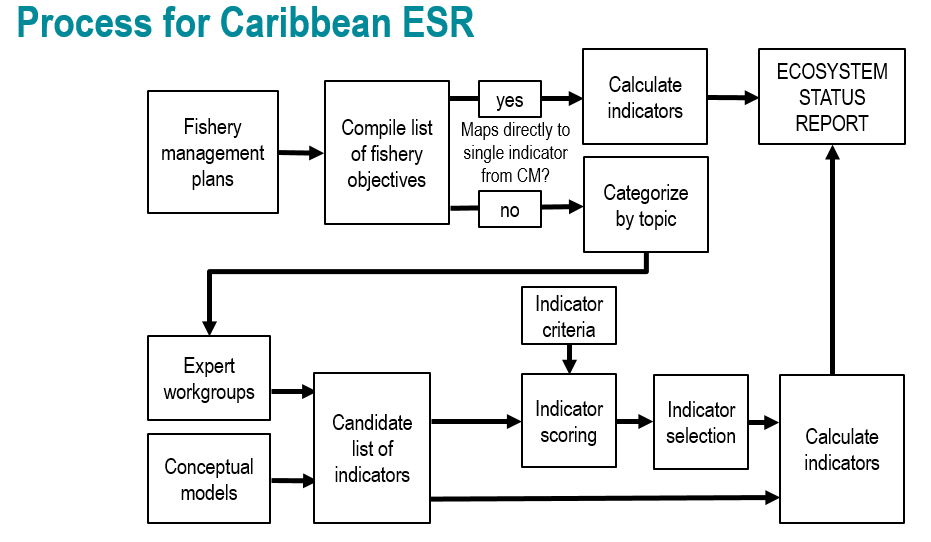
\includegraphics[width=5.36458in,height=\textheight]{images/process_flow_chart.png}

}

\caption{\label{fig-flowchart}Process for selecting indicators for the
U.S. Caribbean Ecosystem Status Report.}

\end{figure}%

This decision matrix was composed of a list of proposed indicators
compiled from the conceptual models as well as proposed indicators
provided via expert input. These potential indicators were vetted and
edited by expert small working groups, who then scored a decision matrix
(Figure~\ref{fig-flowchart}) of potential indicators against the
following decision criteria: long term data availability, measurability,
sensitivity to environmental changes, specificity, spatial and temporal
scalability, relevance to specific FMP objectives, and responsiveness to
management actions.

\section{Notes on interpreting time series
figures}\label{notes-on-interpreting-time-series-figures}

Time series data are plotted in a standardized format for ease of
interpretation (e.g., Figure~\ref{fig-explot}). The x-axis represents
the temporal dimension, which may be monthly, yearly, or irregular time
steps, and the y-axis represents the indicator value in units specified
in the axis label. The dashed horizontal line represents the mean
indicator value across the entire time series, and the solid horizontal
lines denote the mean plus or minus one standard deviation. Red shaded
areas and green shaded areas show years for which the indicator value is
below or above one standard deviation from the mean, respectively. The
blue vertical shaded box highlights the last five years of indicator
values, over which additional metrics are calculated. Black circles to
the right of each figure indicate whether the indicator values over the
last five years are greater (plus sign), less than (minus sign), or
within (solid circle) one standard deviation from the mean of the
overall time series. Arrows to the right of each figure indicate whether
the least squares linear fit through the last five years of data
produces a positive or negative slope that is greater than one standard
deviation (upward or downward arrows respectively), or less than one
standard deviation (left-right arrow).

\begin{figure}

\centering{

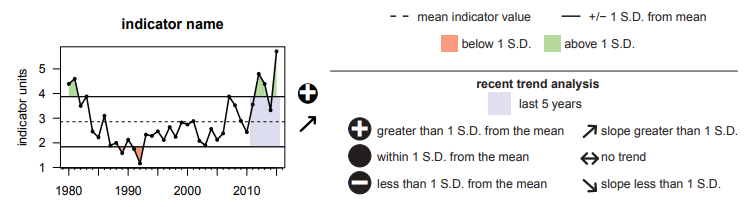
\includegraphics{images/indicator_selection_diagram.png}

}

\caption{\label{fig-explot}Example time series plot, showing an
indicator plotted with its mean and standard deviation, and trend
analysis for the most recent five years of data. See text for more
detailed description of specific calculations.}

\end{figure}%

\bookmarksetup{startatroot}

\chapter{Risks to meeting fishery management
objectives}\label{risks-to-meeting-fishery-management-objectives}

In this section, we examine indicators related to risks to meeting the
Fishery Management Plan objectives.

\section{Sea surface temperature}\label{sea-surface-temperature}

Ocean temperatures affect species distributions and other aspects of
population dynamics and have impacts on habitats such as coral reefs.
Monthly mean, minimum, and maximum sea surface temperatures were
calculated based on the 1/4 Degree Daily Optimum Interpolation Sea
Surface Temperature (OISST) Analysis (Reynolds et al. 2007). Mean
temperatures in the U.S. Caribbean region have been increasing at an
average rate of 0.25 degrees Celsius per decade. In the last five years,
minimum temperatures have been well above average, while there has been
no long-term or recent trend in maximum temperatures experienced
(Figure~\ref{fig-SST}).

\begin{figure}

\centering{

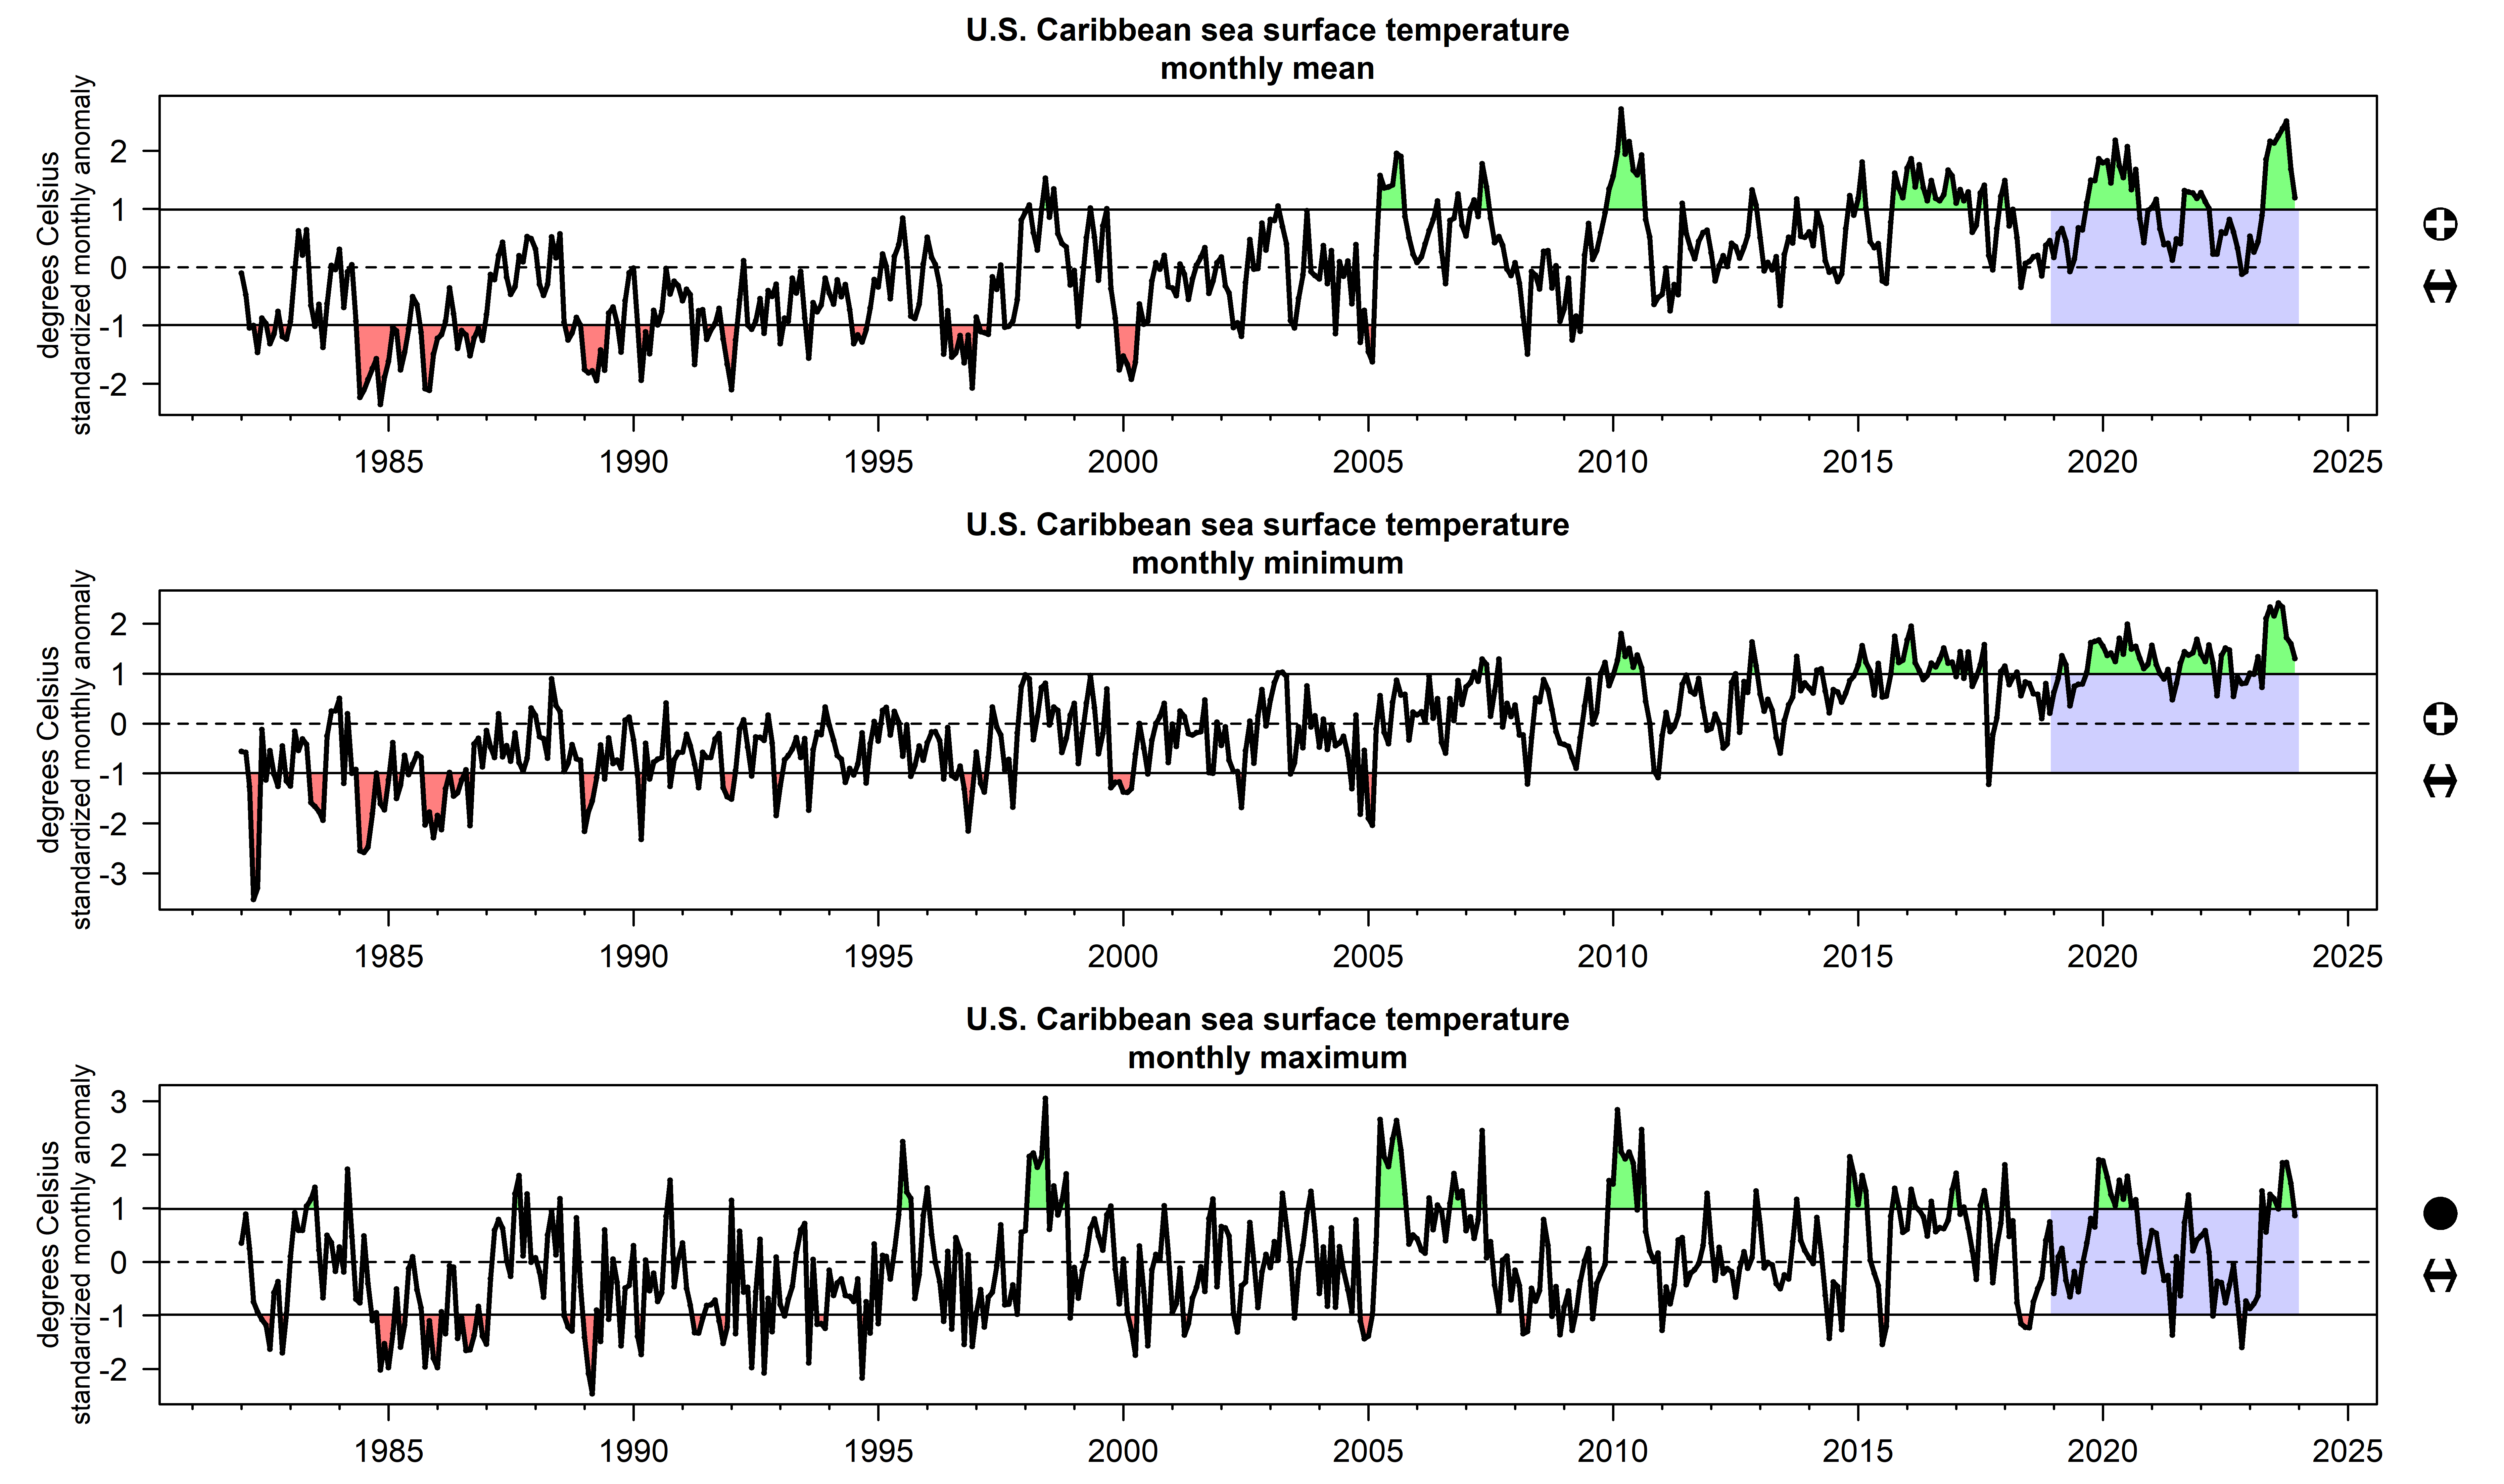
\includegraphics{indicator_plots/Carib_SST_plot_final.png}

}

\caption{\label{fig-SST}Mean, minimum, and maximum sea surface
temperature standardized monthly anomalies for the Puerto Rico and USVI
regions.}

\end{figure}%

\section{Coral bleaching stress}\label{coral-bleaching-stress}

Accumulated heat stress, which can lead to coral bleaching and death, is
measured by summing degree heating weeks for the most recent 12-week
period from sea surface temperature data (NOAA Coral Reef Watch 2019).
Bleaching stress was generally below average until the mid-2000s, until
a sudden bleaching event in 2005 which is now the second most severe
event in history. In 2024, an unprecedented bleaching event occurred
across the U.S. Caribbean and beyond (Figure~\ref{fig-DHW}).

\begin{figure}

\centering{

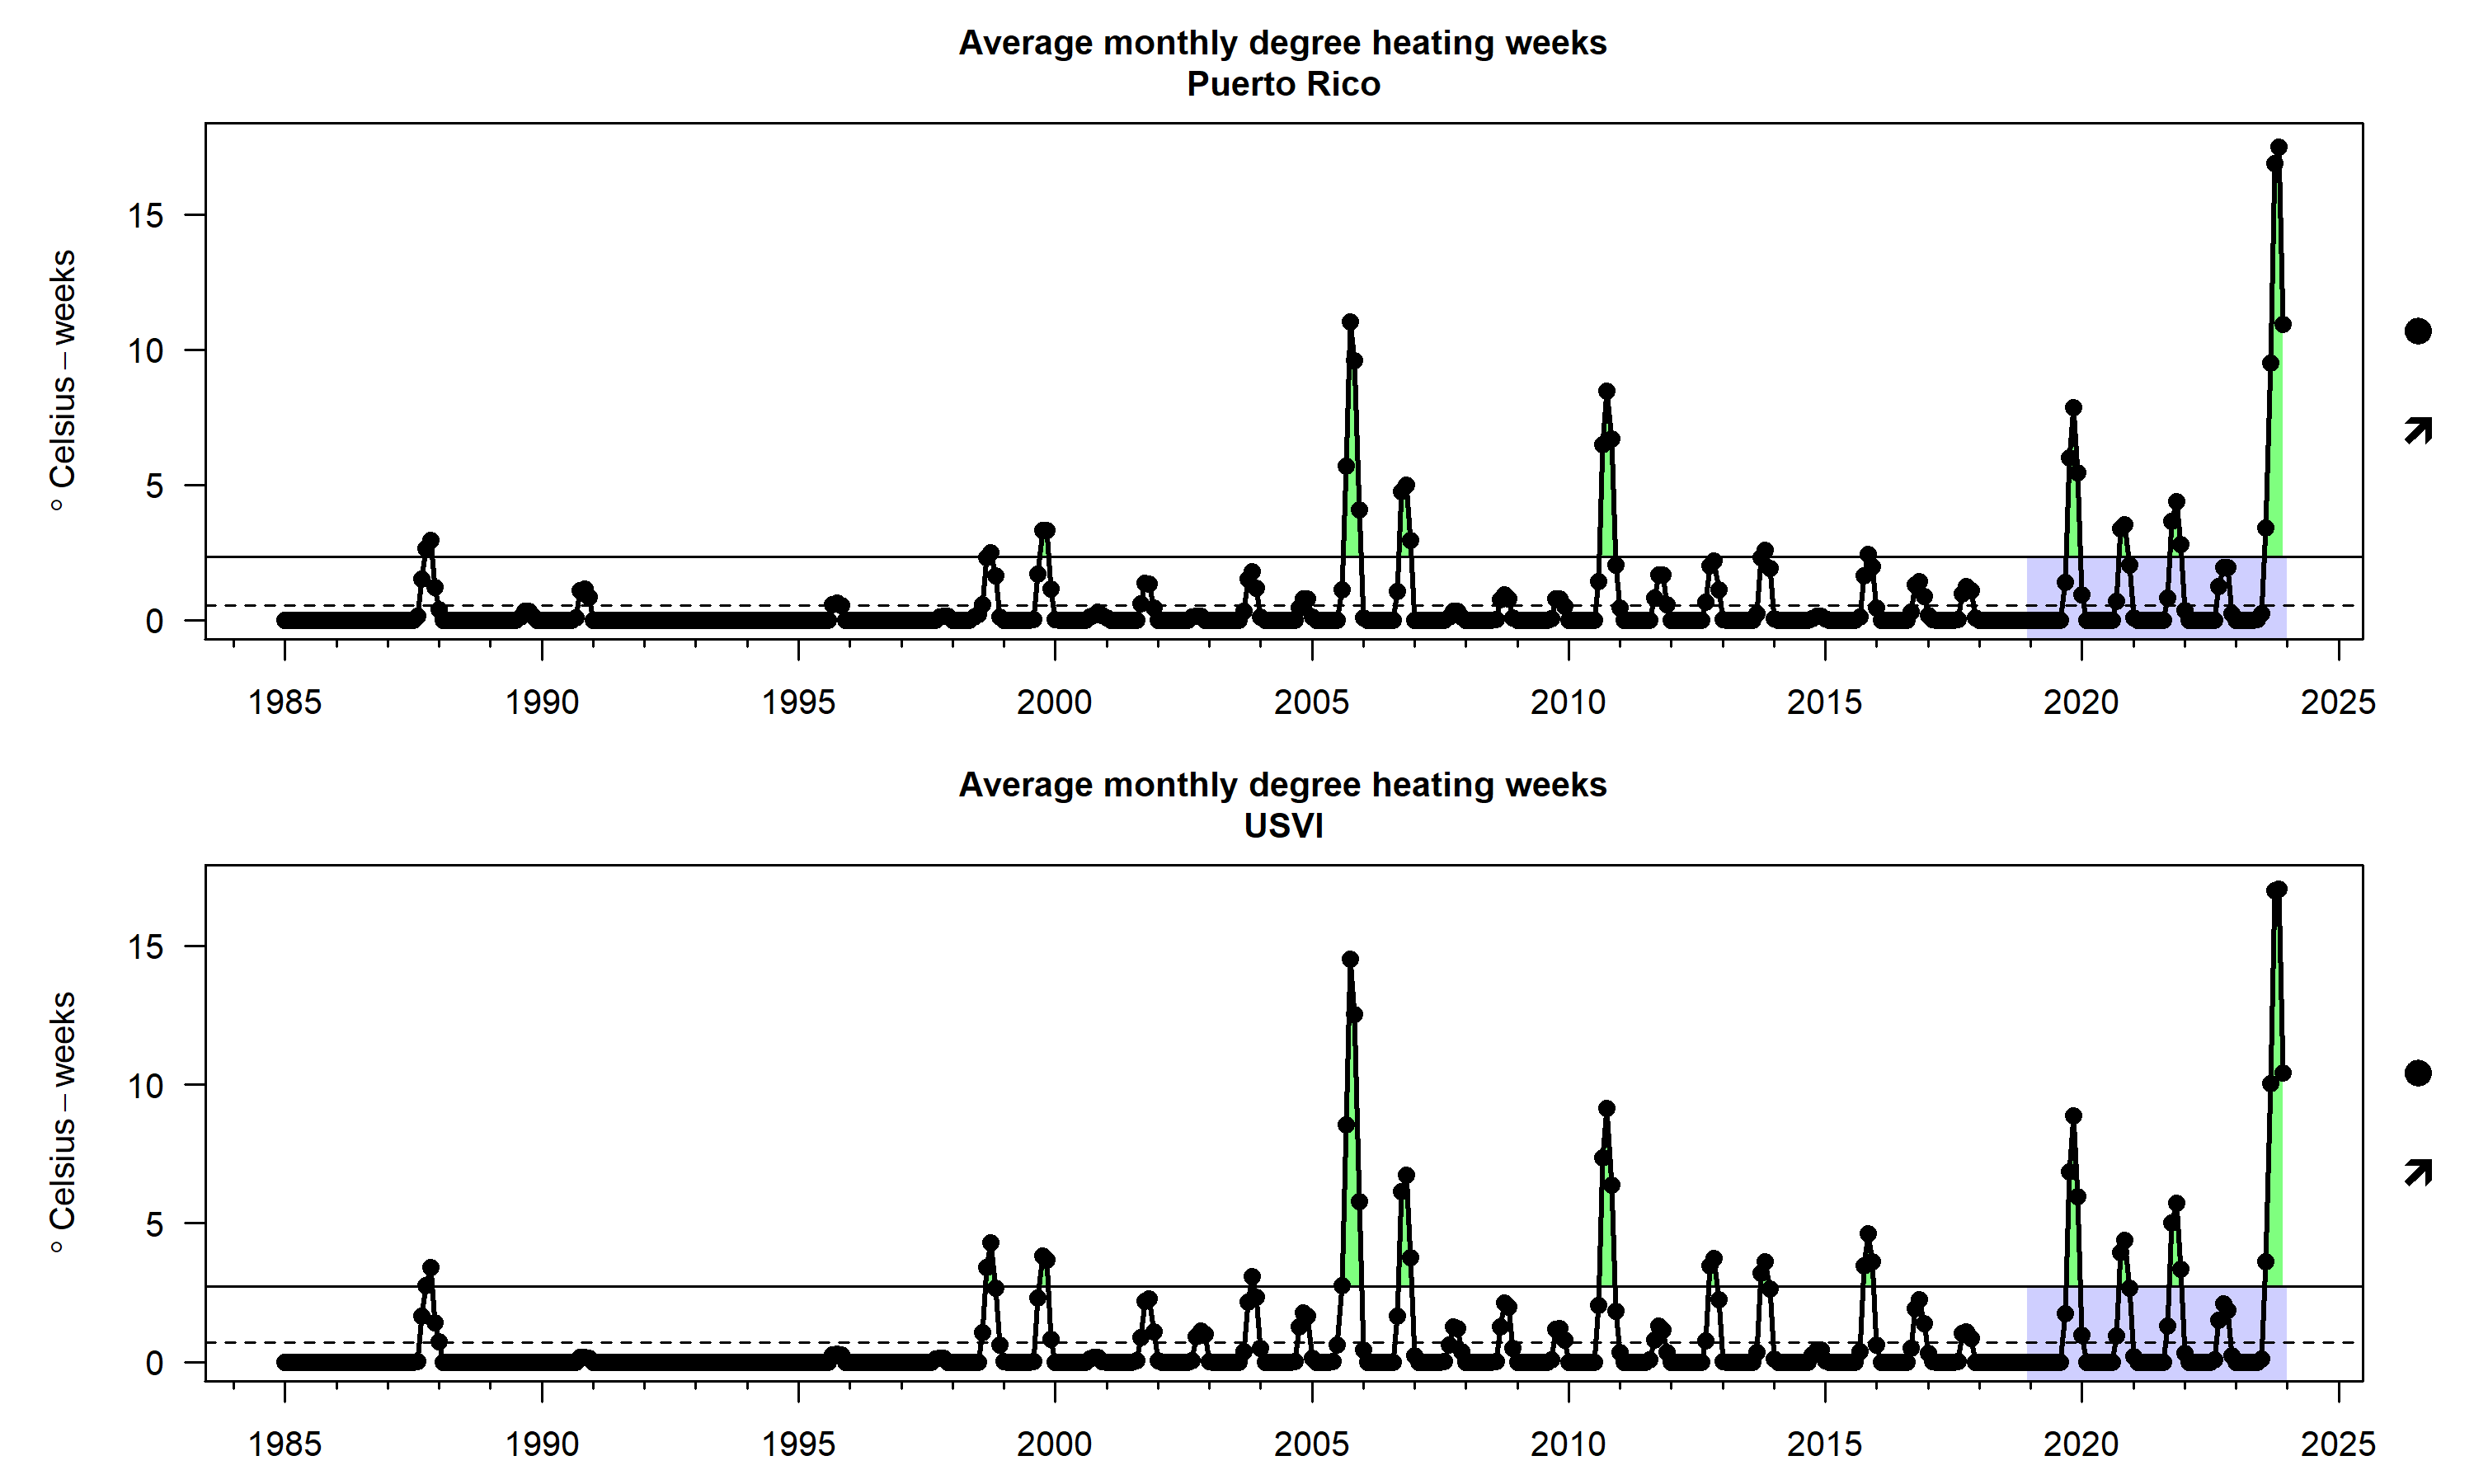
\includegraphics{indicator_plots/DegreeHeatingWeeks_plot_final.png}

}

\caption{\label{fig-DHW}Number of degree heating weeks in Puerto Rico
and the USVI as a measure of thermal stress to corals.}

\end{figure}%

\section{Ocean acidification via aragontite saturation
state}\label{ocean-acidification-via-aragontite-saturation-state}

Ocean and coastal acidification can impact organisms directly or
indirectly; a decrease in aragonite saturation state can weaken the
structure of coral reefs and other calcifying organisms. In-situ
measurements of aragonite saturation states are scarce and a synoptic,
long-term view is only available from modeled products. Aragonite
saturation state was derived for the U.S. Caribbean region from the
MOM-TOPAZ hindcast (cite). An overall negative trend occurs, with an
acceleration of this trend apparent after 2008 (Figure~\ref{fig-OA}).

\begin{figure}

\centering{

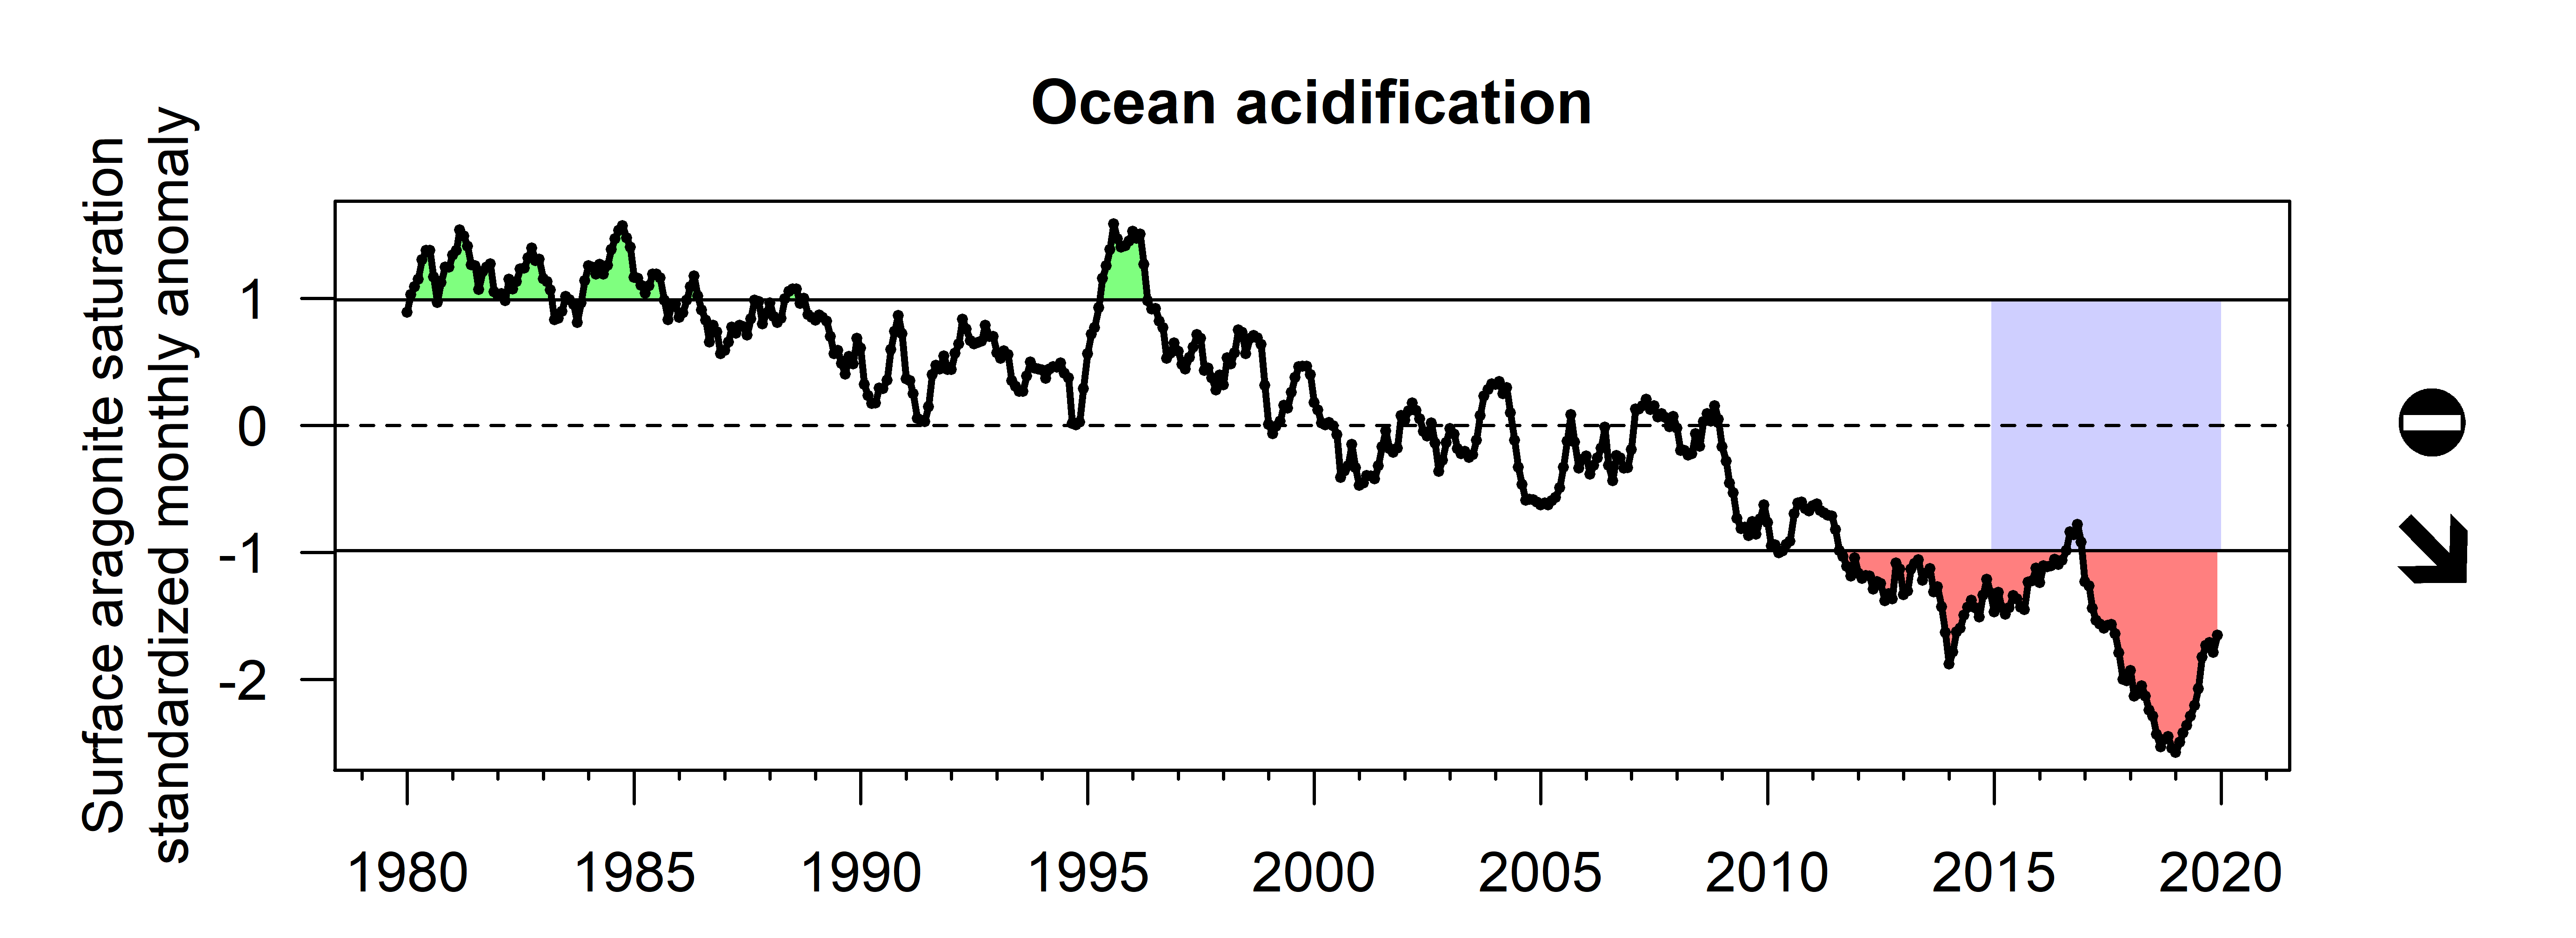
\includegraphics{indicator_plots/OA_plot_final.png}

}

\caption{\label{fig-OA}Ocean acidification plot}

\end{figure}%

\section{Hurricane activity}\label{hurricane-activity}

Hurricane activity can be captured by the accumulated cyclone energy
index which is calculated as the sum of squared wind speeds for storms
tracking through the U.S. Caribbean region, as documented by the
International Best Track Archive for Climate Stewardship database (Knapp
et al. 2010). The index has fluctuated throughout the past seven
decades, with multiple notable peaks (Figure~\ref{fig-ACE}). The year
2017 hurricane activity was at an unprecedented high, due to two major
hurricanes that struck the islands: Irma and Maria.

\begin{figure}

\centering{


\includegraphics{indicator_plots/ACEindex_plot_final.png}

}

\caption{\label{fig-ACE}Annual accumulated cyclone energy index,
calculated as the sum of squared 6-hourly reported wind speeds for
storms tracking through the U.S. Caribbean region.}

\end{figure}%

\section{Number of major earthquakes}\label{number-of-major-earthquakes}

Earthquakes in Puerto Rico can induce landslides and cause impacts to
infrastructure including homes and the electrical grid, and can be a
source of stress in the affected human population (Agar et al. 2022).
Seismic events are reported by the USGS in near real-time (Sumy, Welti,
and Hubenthal 2020). A major earthquake swarm occurred in Southwest
Puerto Rico in early 2020; in this year there were over 400 events of
greater than 3.5 magnitude on the Richter scale
(Figure~\ref{fig-quakes}).

\begin{figure}

\centering{

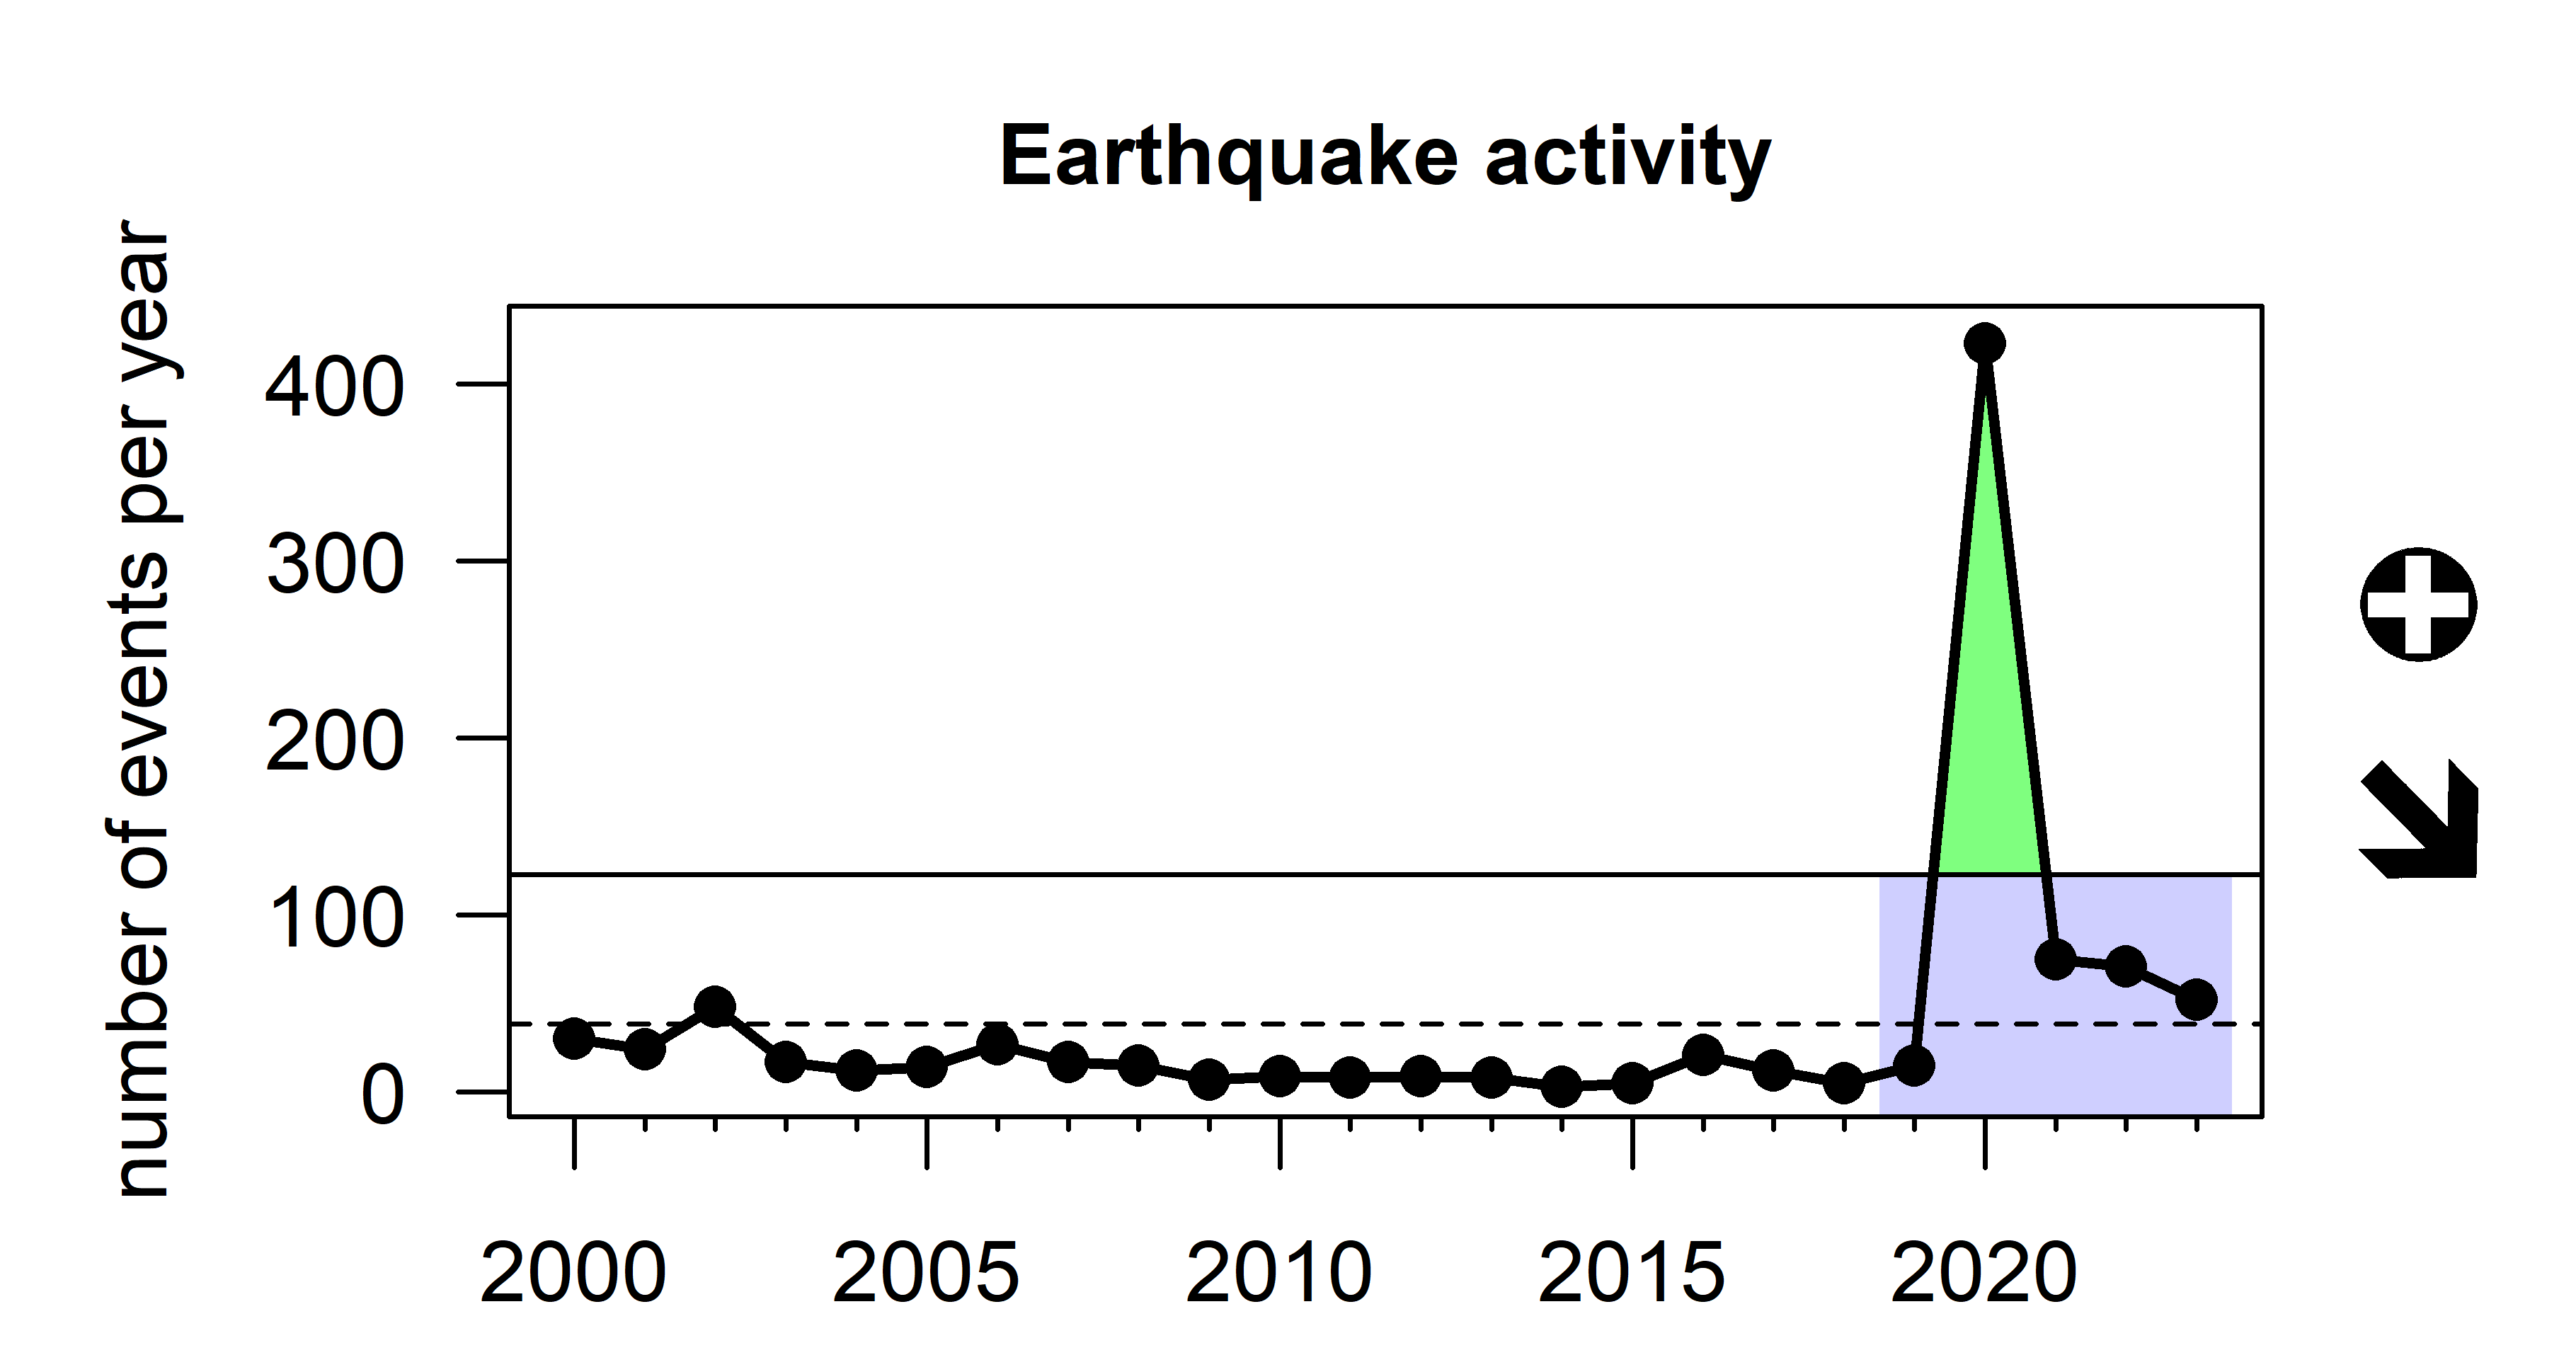
\includegraphics{indicator_plots/earthquakes_plot_final.png}

}

\caption{\label{fig-quakes}The number of seismic events \textgreater3.5
in the U.S. Caribbean, 1970-2023.}

\end{figure}%

\section{Identified point source pollution
sites}\label{identified-point-source-pollution-sites}

Impacts from terrestrial pollution can be captured from several
databases maintained by the Environmental Protection Agency, which
provide information on companies that have been issued permits to
discharge wastewater into rivers, release of toxic chemicals and waste
management activities at facilities, and declaration of Superfund sites.
The number of pollution sites reported increased in the 2000s, but has
decreased slightly in both Puerto Rico and USVI in recent years
(Figure~\ref{fig-pollution}). Note that this indicator does not
represent the timing of when pollution was impacting the ecosystem, but
rather the timing of political action or attention on the environmental
impacts of pollution.

\begin{figure}

\centering{

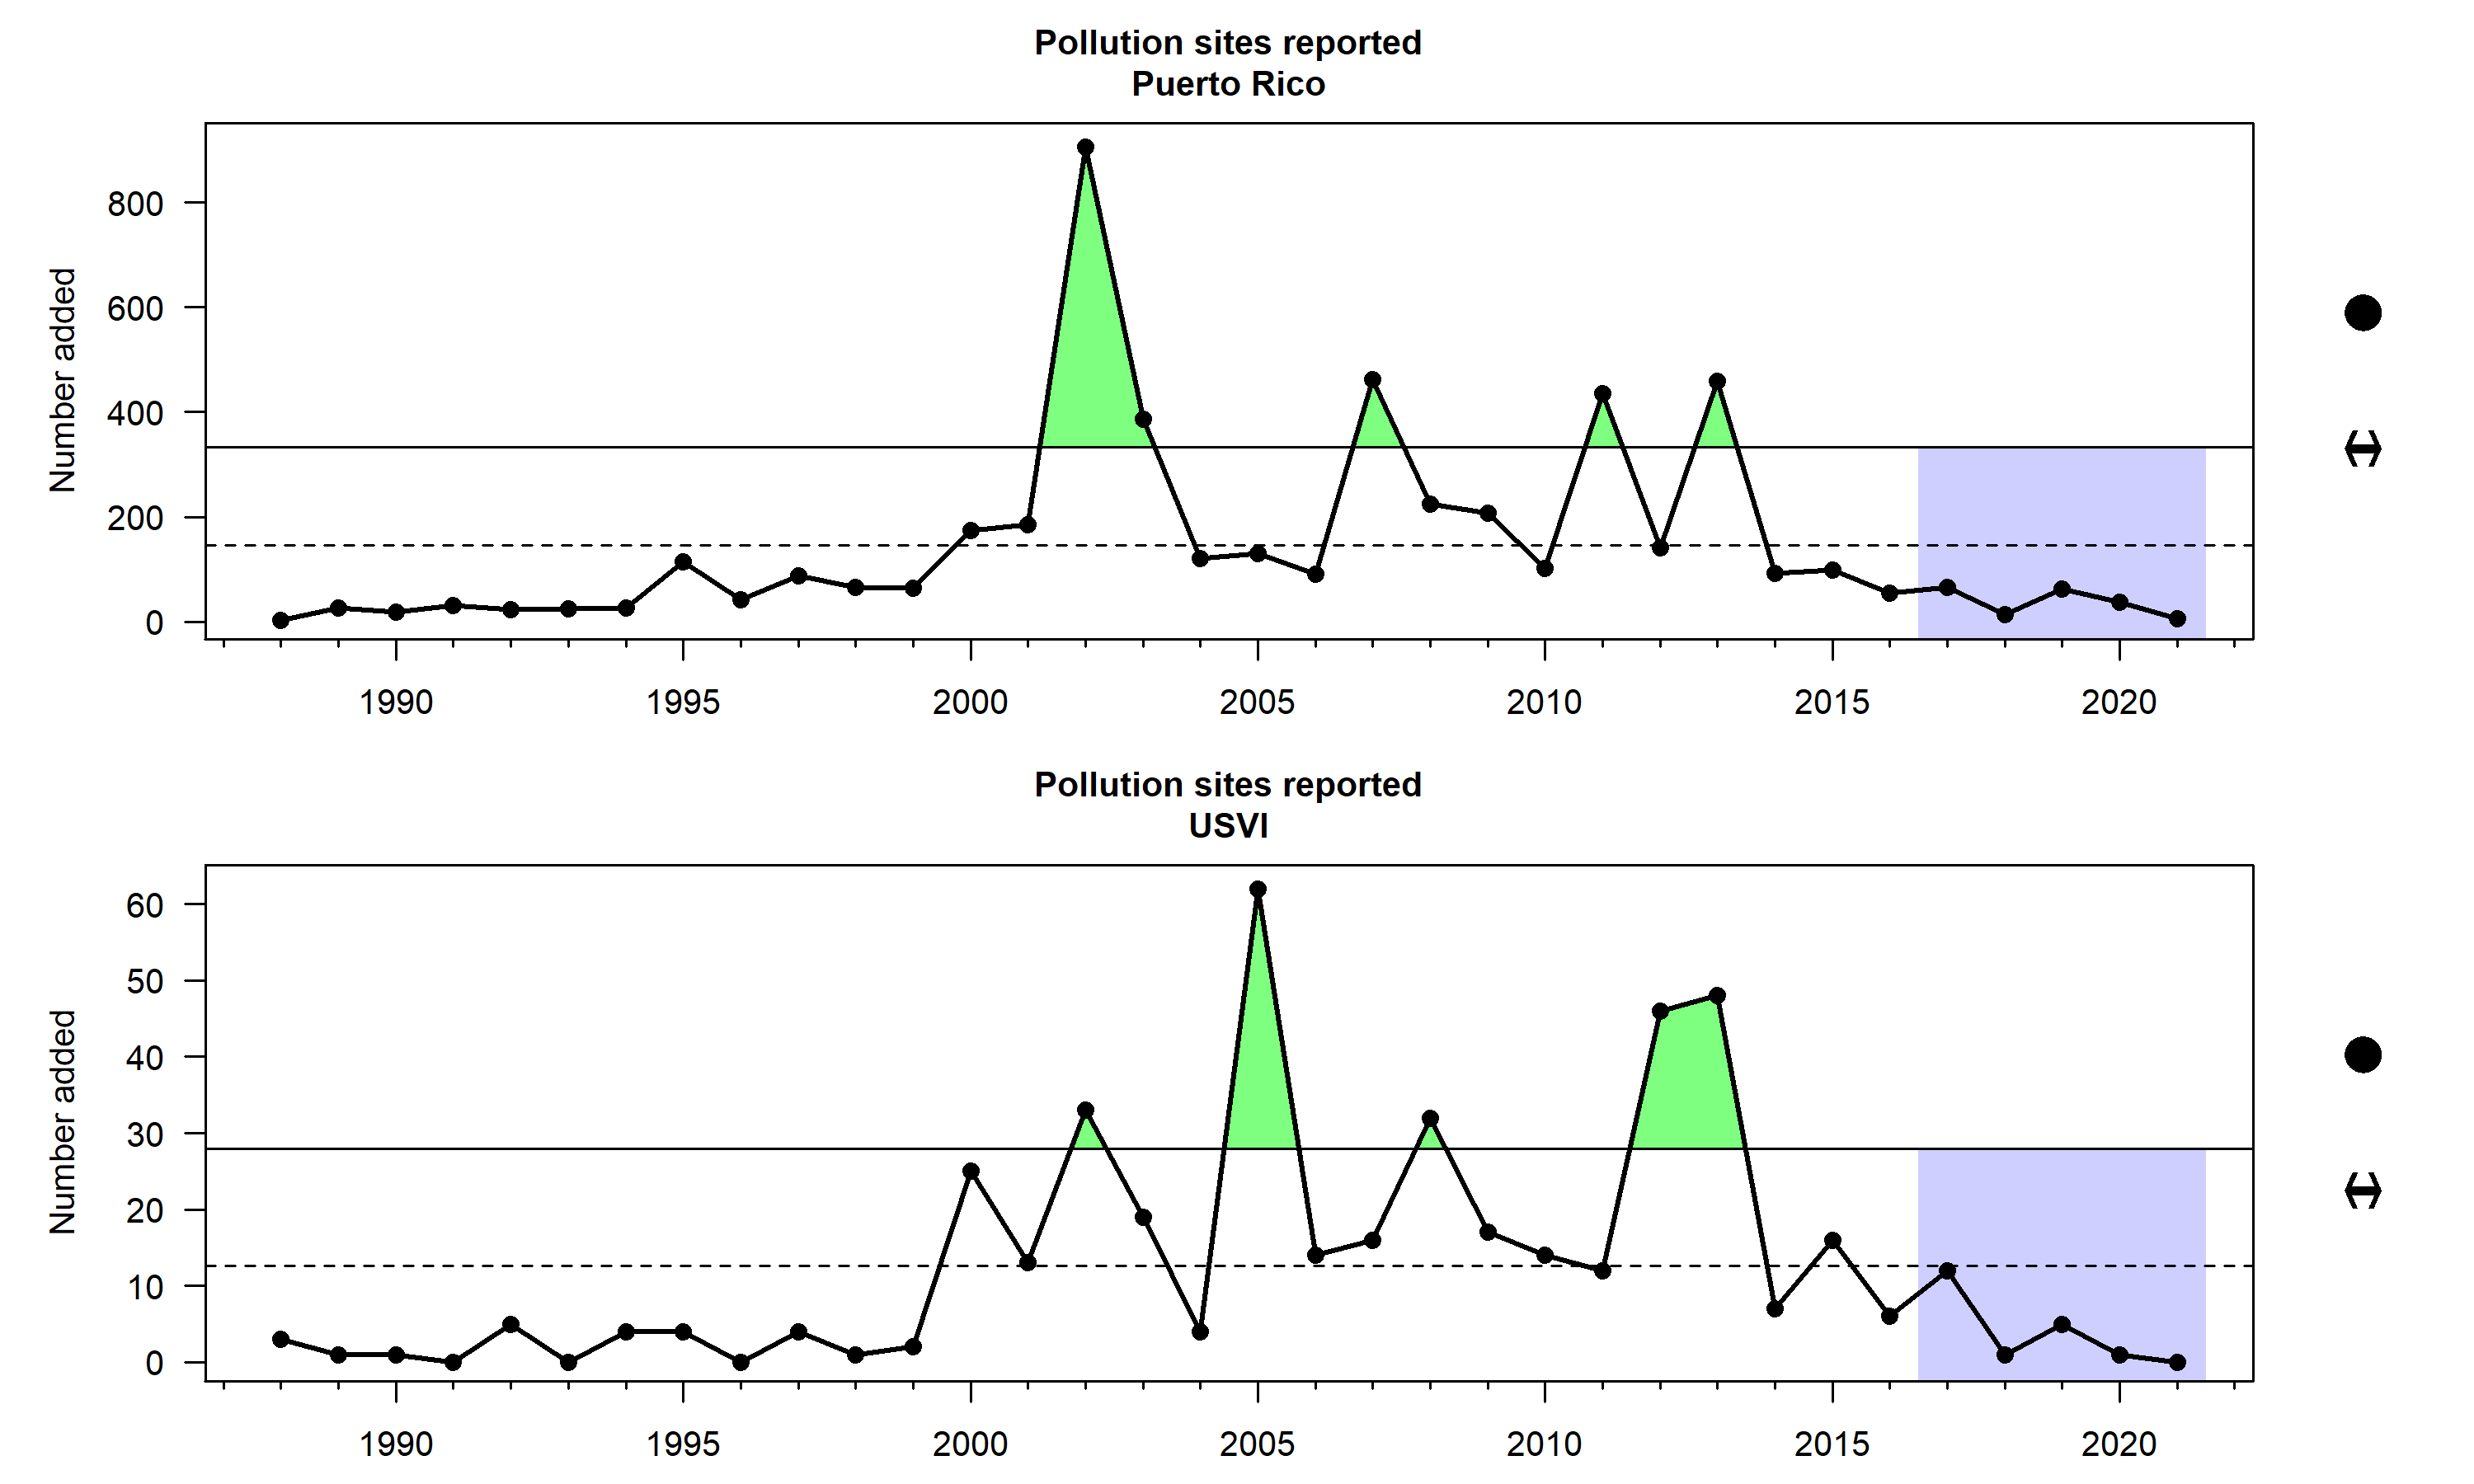
\includegraphics{indicator_plots/pollution_plot_final.png}

}

\caption{\label{fig-pollution}Annual count of identified point source
polluters in the U.S. Caribbean: TRI sites (Toxic Release Inventory),
Superfund sites (Superfund Enterprise Management System), National
Compliance Database listed sites, and Brownfield sites identified in the
U.S. Caribbean.}

\end{figure}%

\section{Turbidity}\label{turbidity}

Coastal pollution, runoff, and water quality issues are of major concern
to fishing-dependent communities in the U.S. Caribbean (Seara et al.
2024). Water clarity can be measured by the diffuse attenuation
coefficient which indicates how strongly light intensity is attenuated
within the water column; however, satellite sensors cannot differentiate
between organic and inorganic water particles contributing to water
clarity. NOAA's Coastwatch program provides estimates of the attenuation
coefficient for penetration of light at 490nm (Wang, Son, and Harding
Jr. 2009) based on multiple satellite sensors. (sentence on trends)

\begin{figure}

\centering{

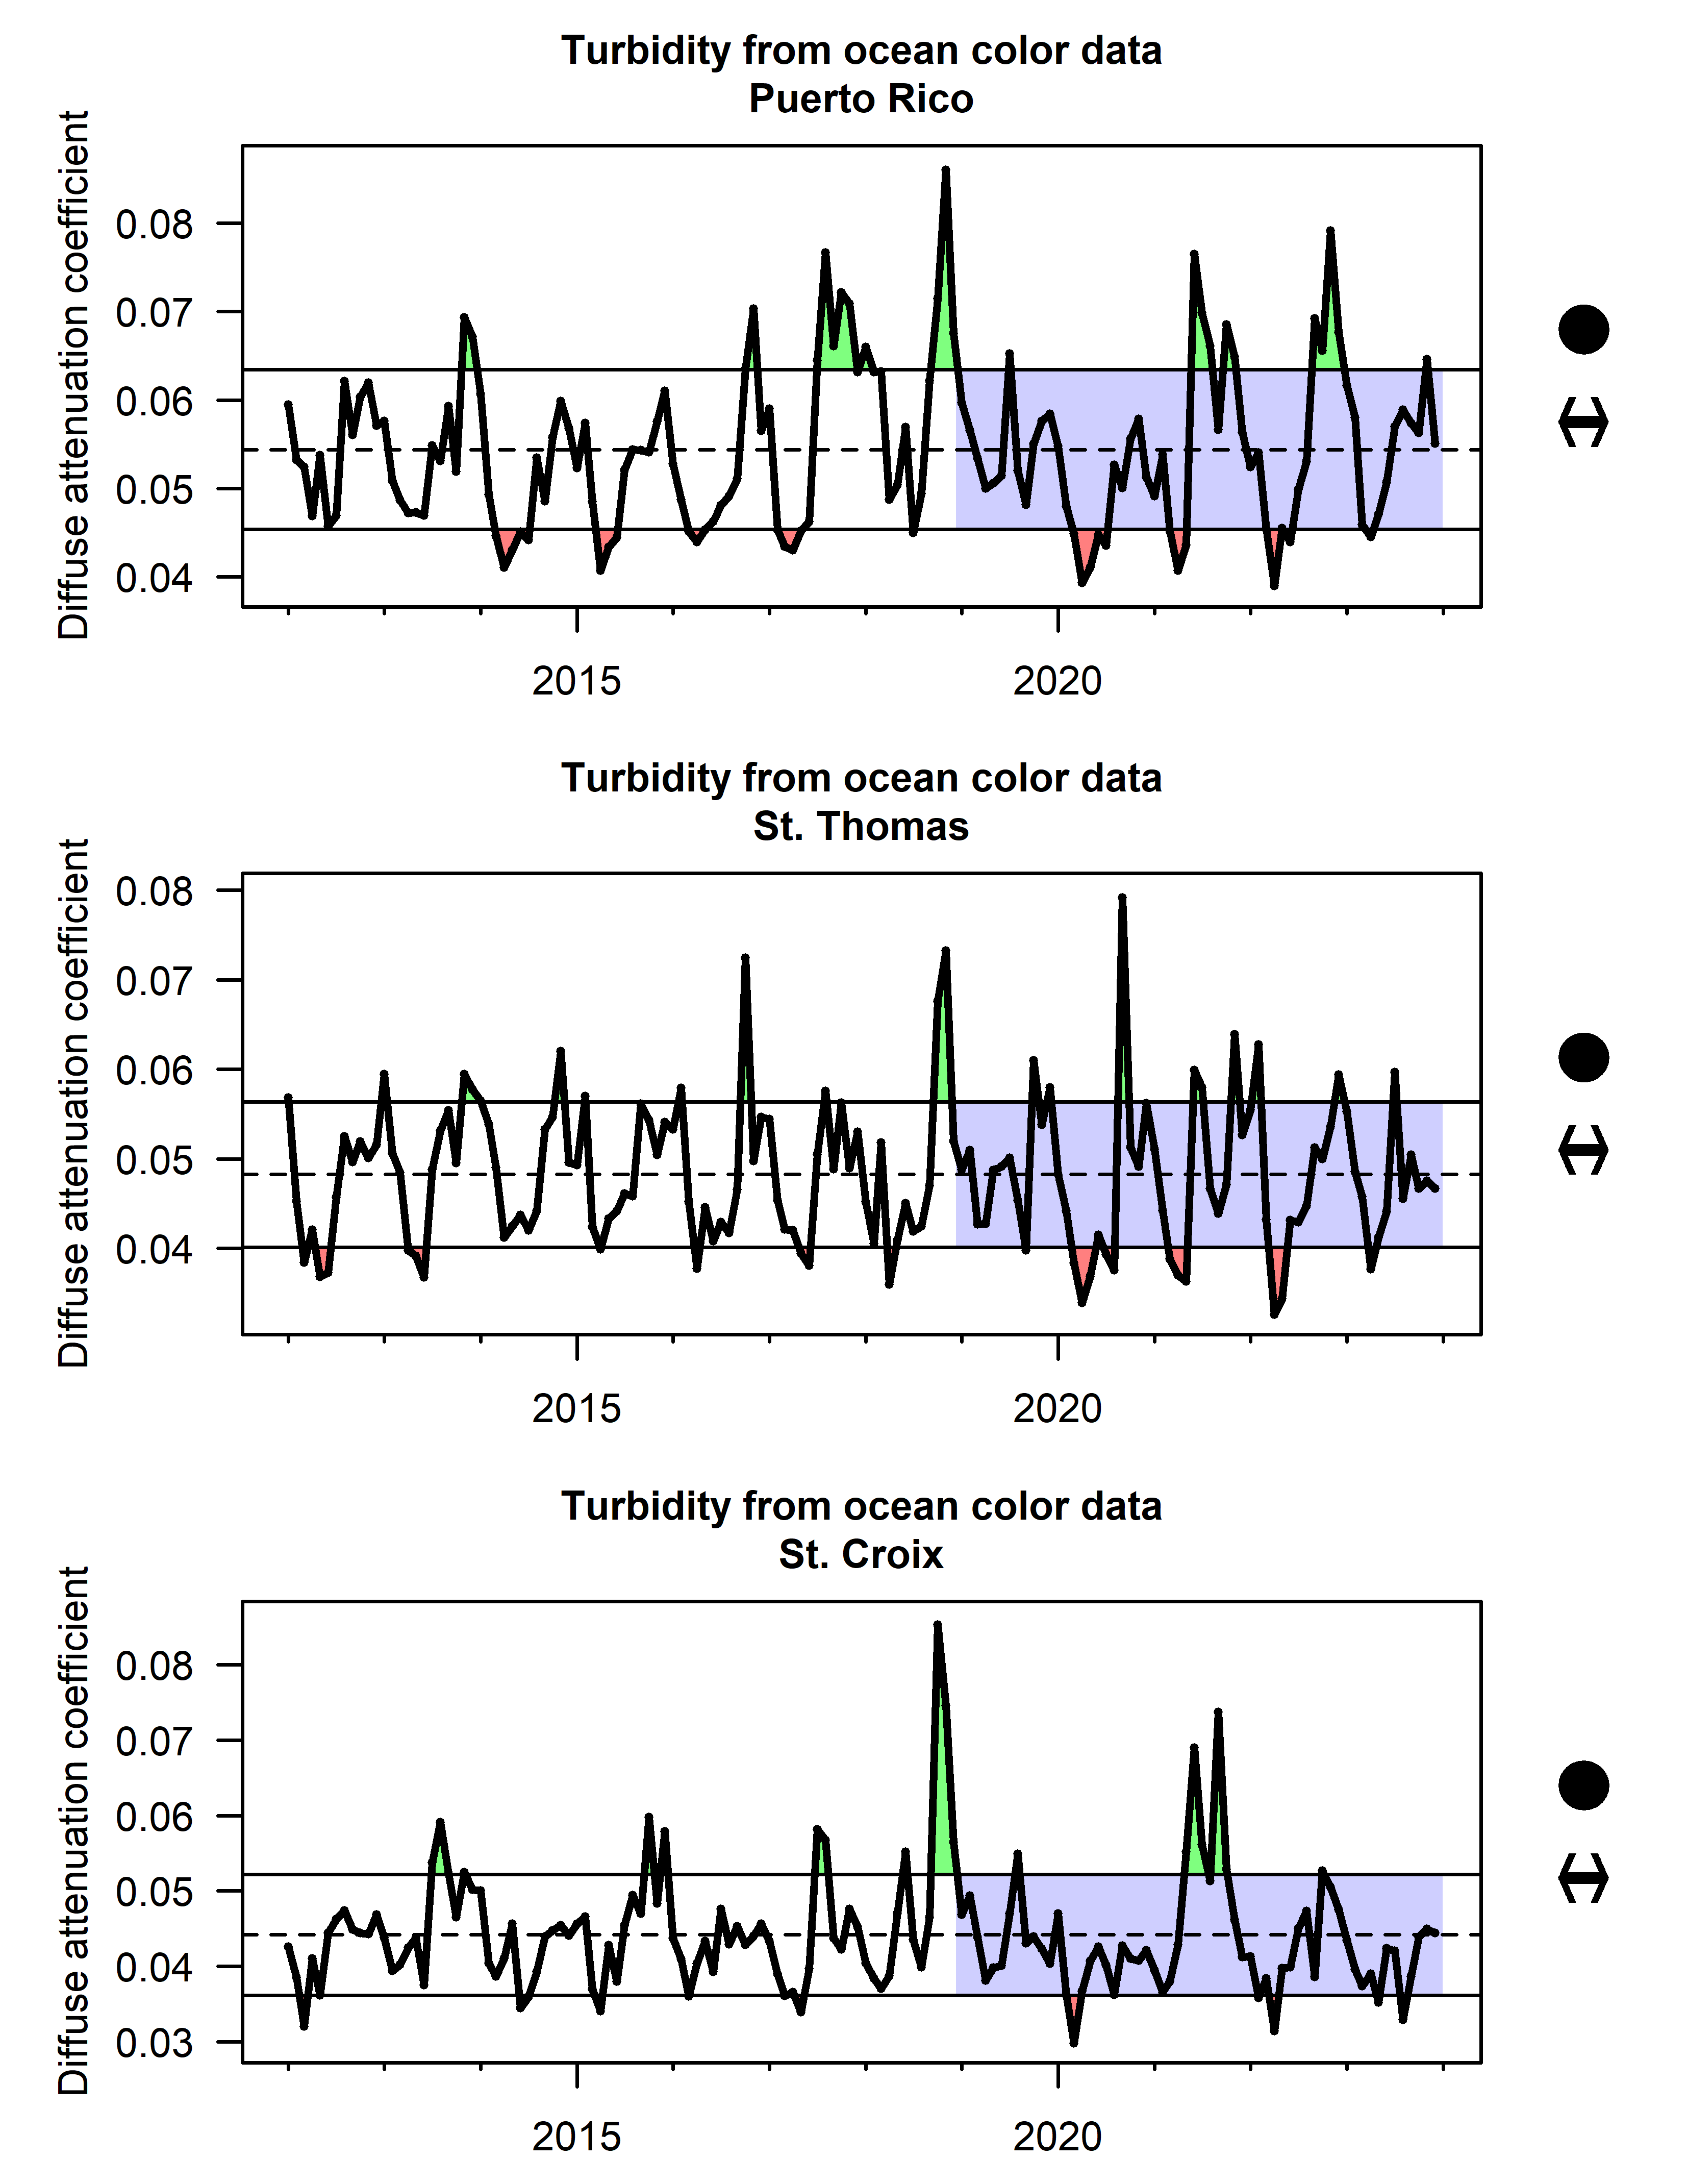
\includegraphics{indicator_plots/turbidity_plot_final.png}

}

\caption{\label{fig-turb}Water turbidity as measured by the diffuse
attenuation coefficient, via monthly Kd490 data from the VIIRS
Coastwatch satellite.}

\end{figure}%

\section{Water quality}\label{water-quality}

WORKING ON THIS ONE

\section{Coastal development}\label{coastal-development}

Impervious surfaces such as pavement, sidewalks, roofs and roads, as
well as other forms of development, reduce the infiltration of water
into the ground. Impervious surfaces often contribute to higher storm
water runoff, greater sediment yields into coastal areas, and increased
pollutant loads, all of which can degrade water quality (NOAA Digital
Coast). This indicator influences water quality and turbidity in
nearshore coastal habitat areas. The highest amount of impervious
surfaces is seen in the San Juan metropolitan area
(Figure~\ref{fig-landuse}).

\begin{figure}

\centering{

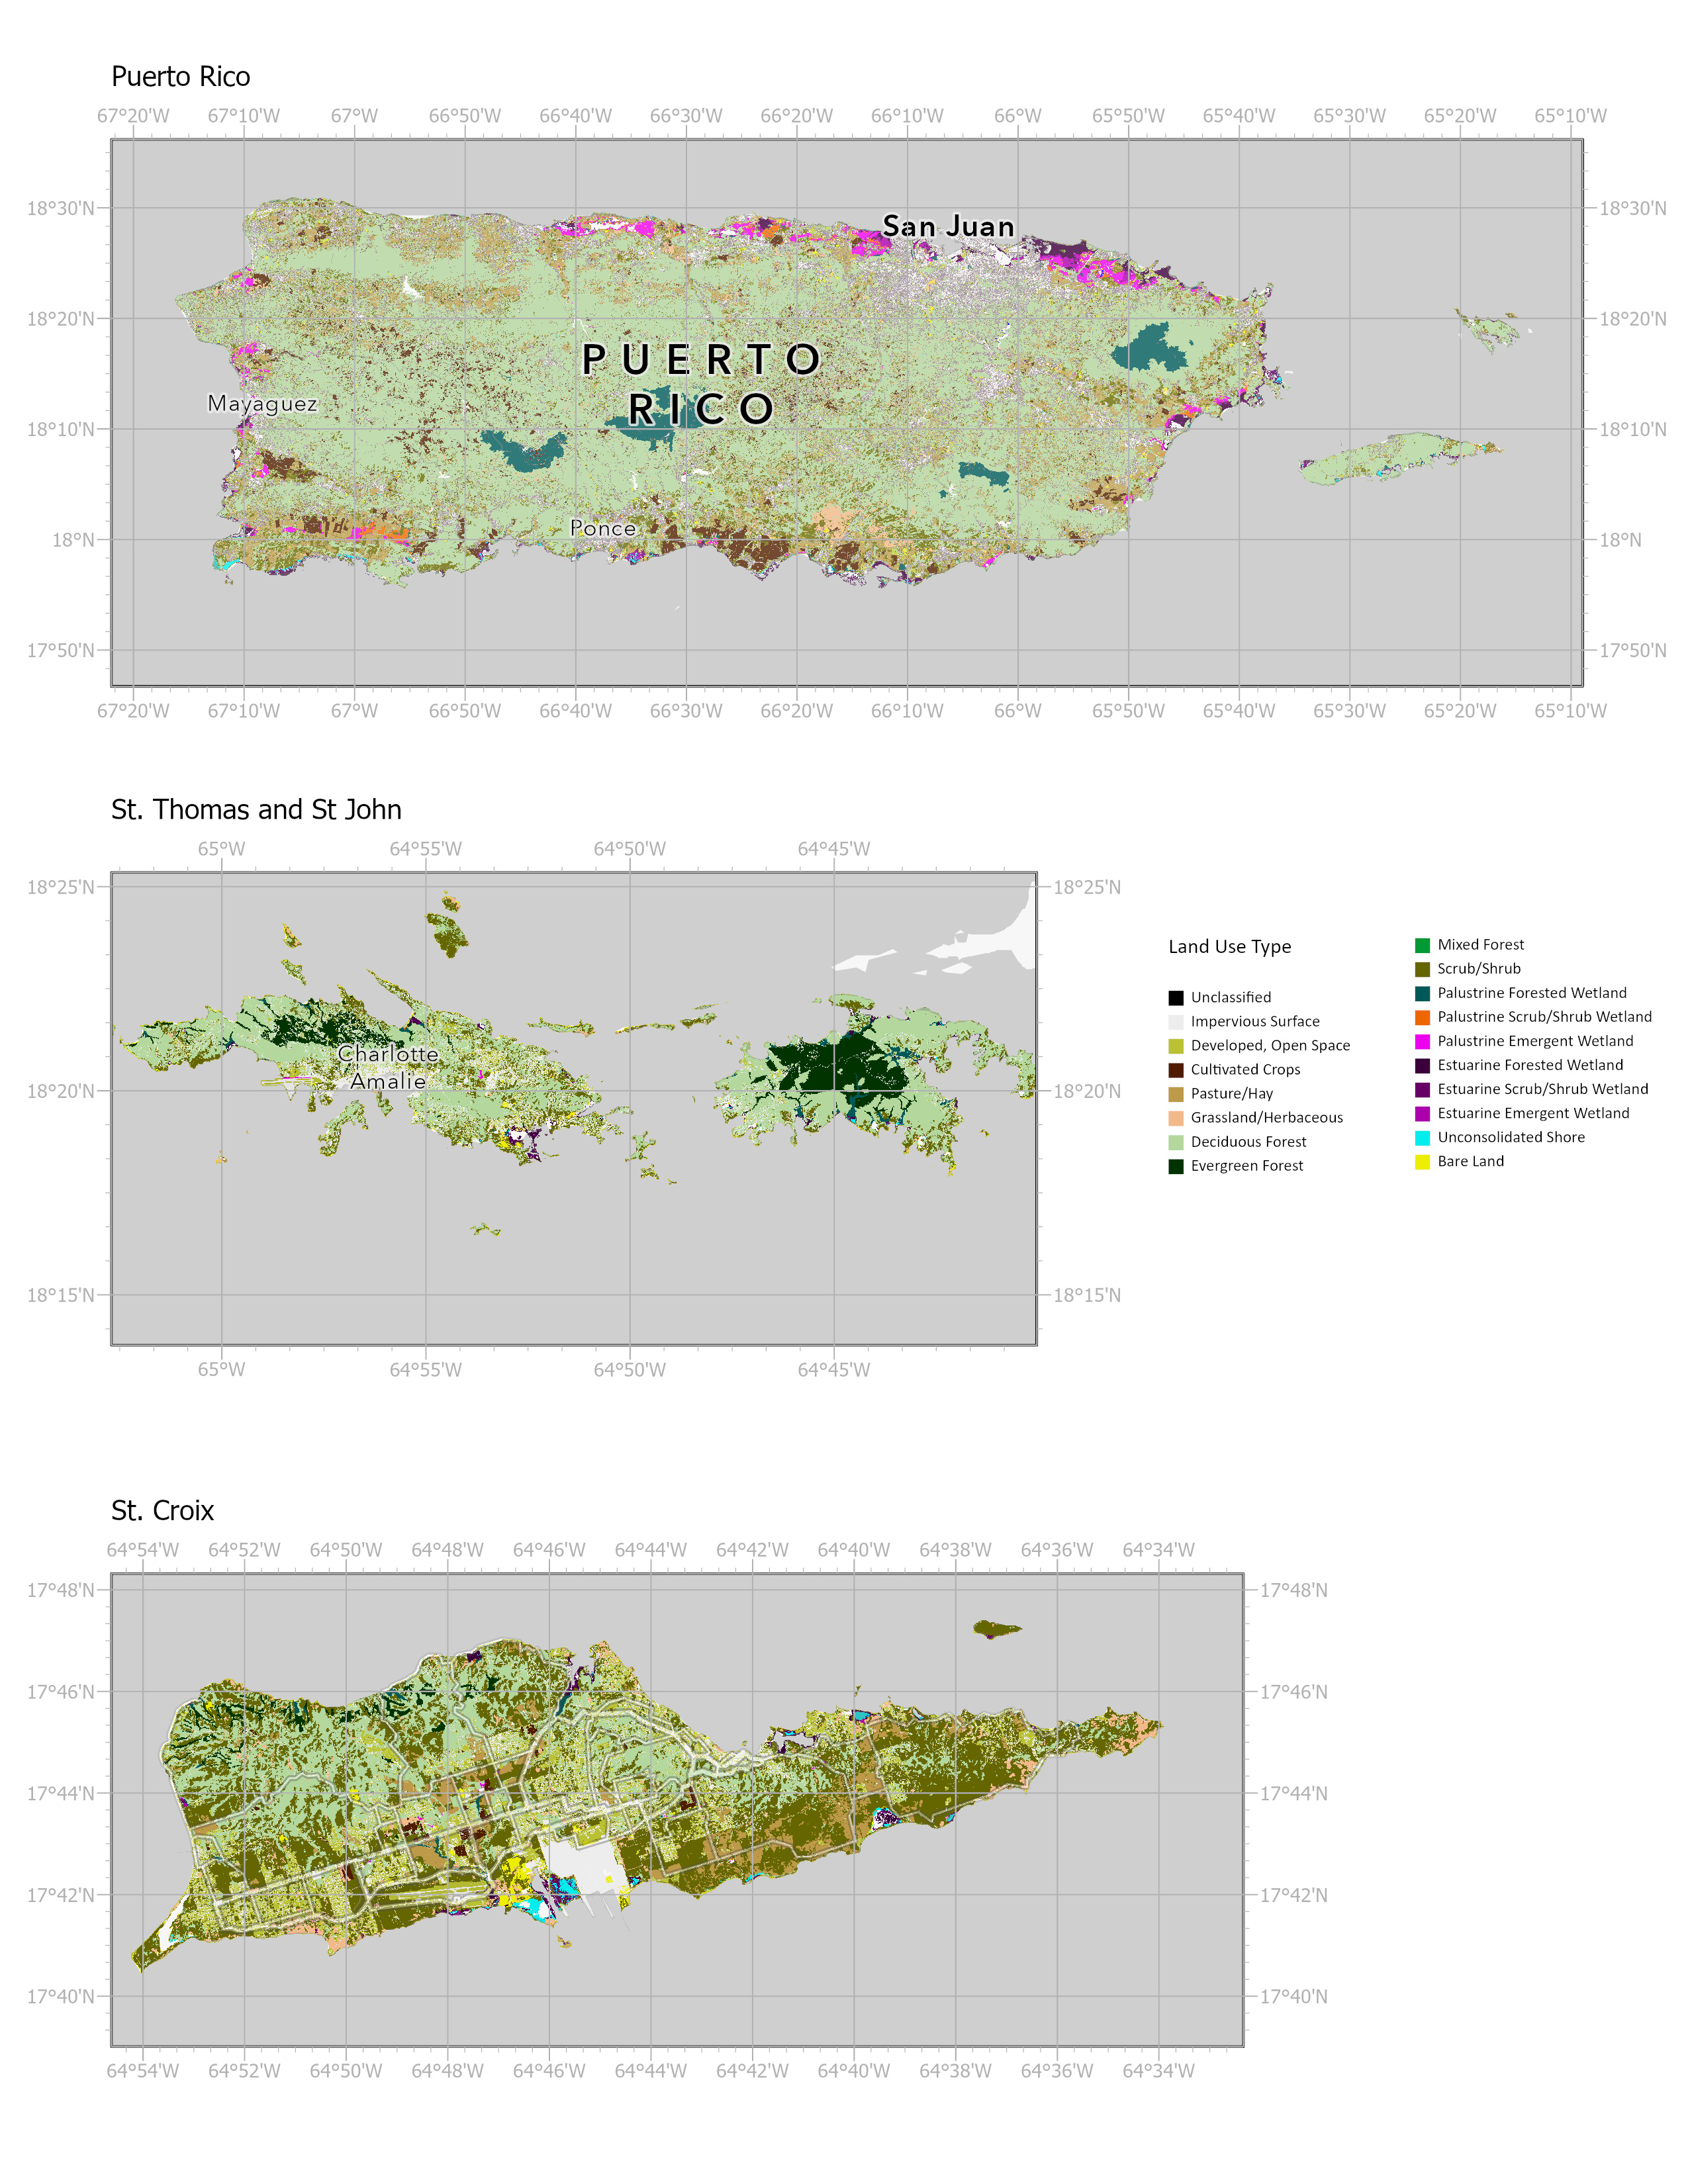
\includegraphics{indicator_plots/Land_Use_Land_Cover_2024.jpg}

}

\caption{\label{fig-landuse}Impervious surfaces from development in the
U.S. Caribbean.}

\end{figure}%

\section{Primary productivty via ocean
color}\label{primary-productivty-via-ocean-color}

Primary productivity is a measure of the total energy available in an
ecosystem and is closely correlated with chlorophyll a concentrations.
Average chlorophyll a concentrations are derived from the European Space
Agency Climate Change Initiative's Ocean Colour product which provides a
bias-corrected composite of measurements merged from multiple satellite
sensors (Hu, Lee, and Franz 2012). Concentrations are plotted as
standardized monthly anomalies as there is a seasonal signal that could
mask long-term trends. Estimates show a decadal cyclical pattern, with
no overall or recent trend apparent (Figure~\ref{fig-chl}).

\begin{figure}

\centering{

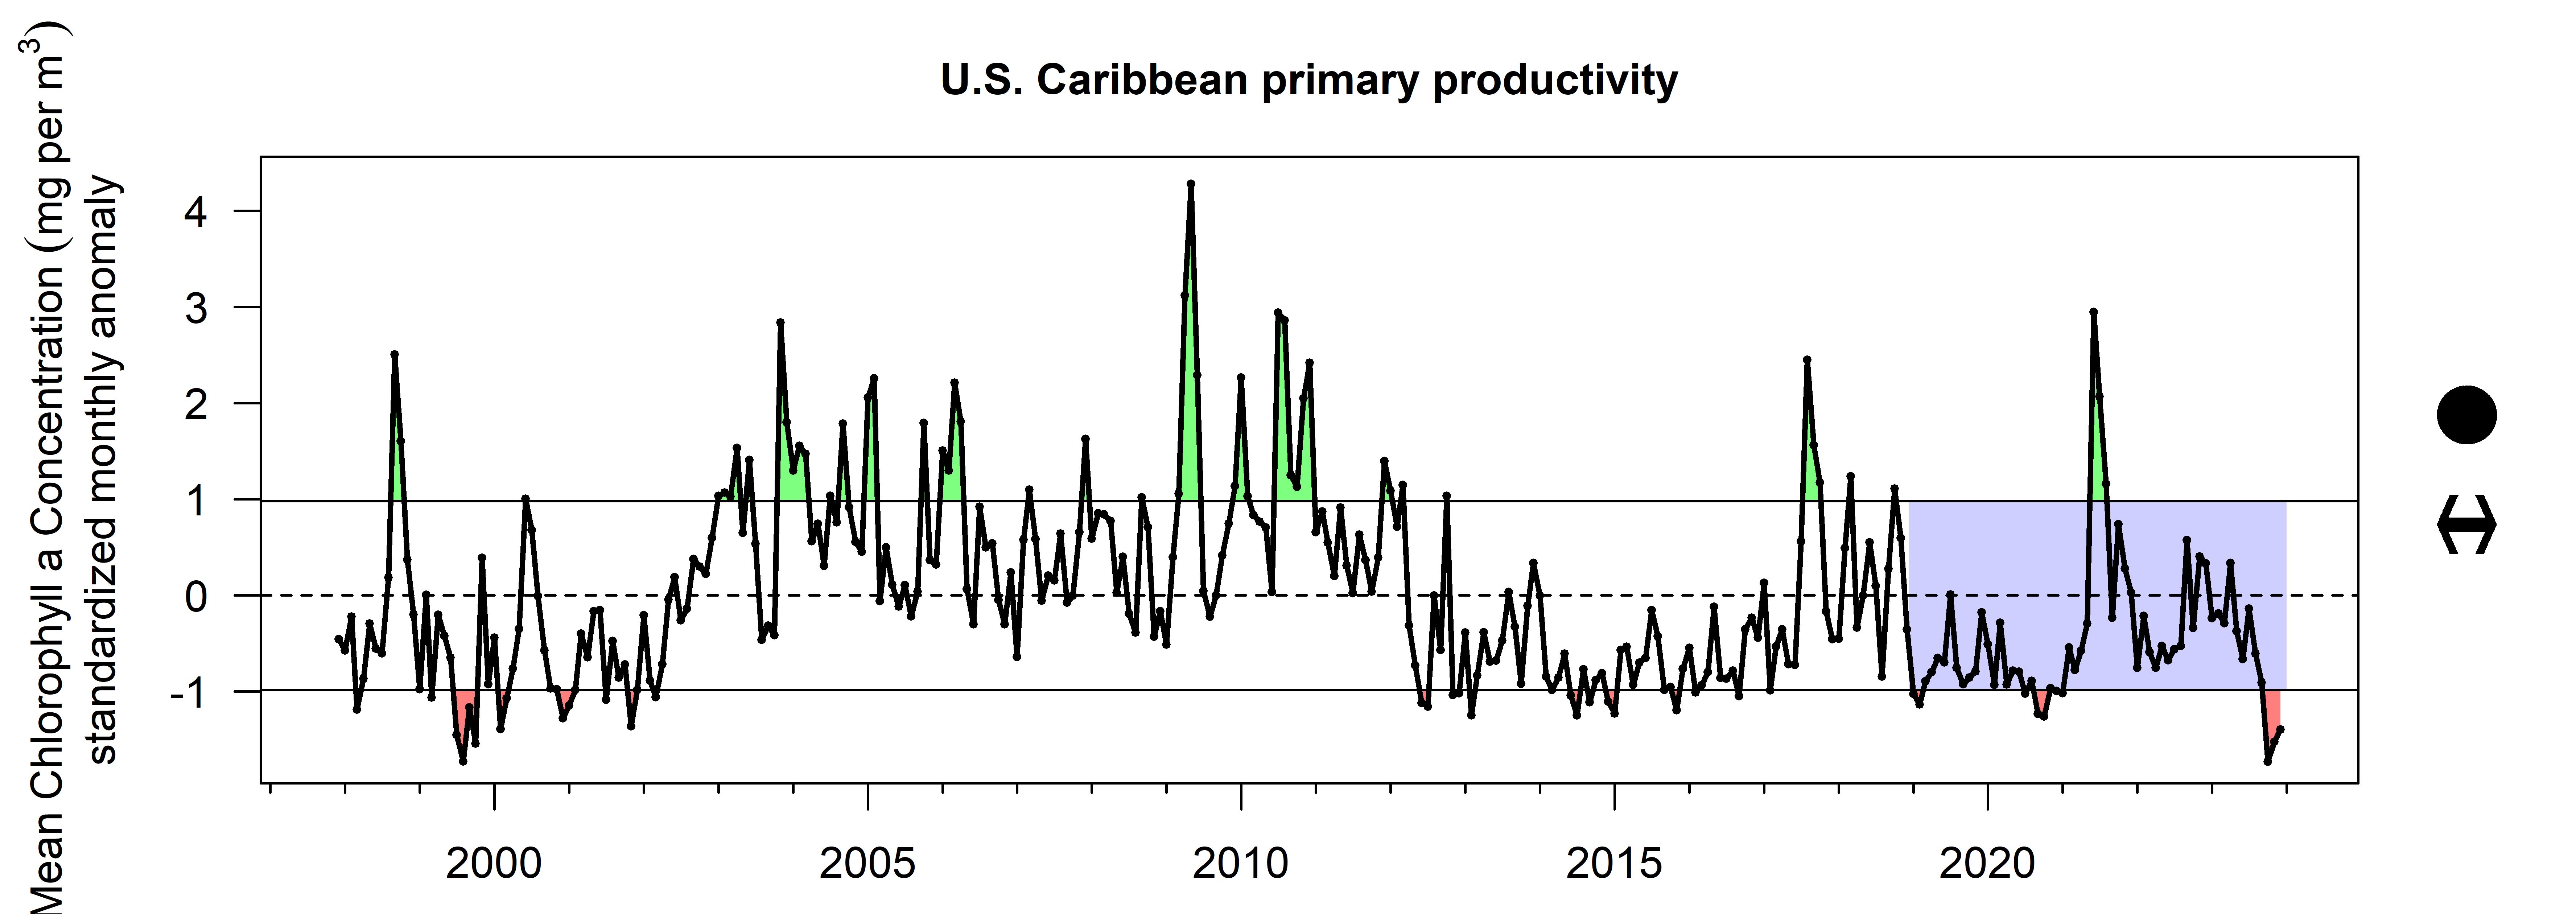
\includegraphics{indicator_plots/carib_Chl_plot_final.png}

}

\caption{\label{fig-chl}Changes in ocean color showing monthly maximum
chlorophyll a levels (standardized monthly anomalies) in the U.S.
Caribbean region.}

\end{figure}%

\section{Sargassum innundation}\label{sargassum-innundation}

Sargassum (brown macroalgae \emph{S. Fluitains} and \emph{S. natans}) is
a designated essential fish habitat important for many pelagic fish and
protected species; however, when large blooms collect in nearshore
environments the mats can reduce oxygen, suffocate beaches and have
detrimental impacts on marine species. Mean monthly Sargassum wet
biomass is estimated from satellite measurements using the algorithm of
Wang et al. (2019). Sargassum blooms were largely absent from the U.S.
Caribbean prior to 2011, but bloom activity has been generally
increasing since that year (Figure~\ref{fig-sarg}). Major inundation
events occurred in 2018 and 2021.

\begin{figure}

\centering{

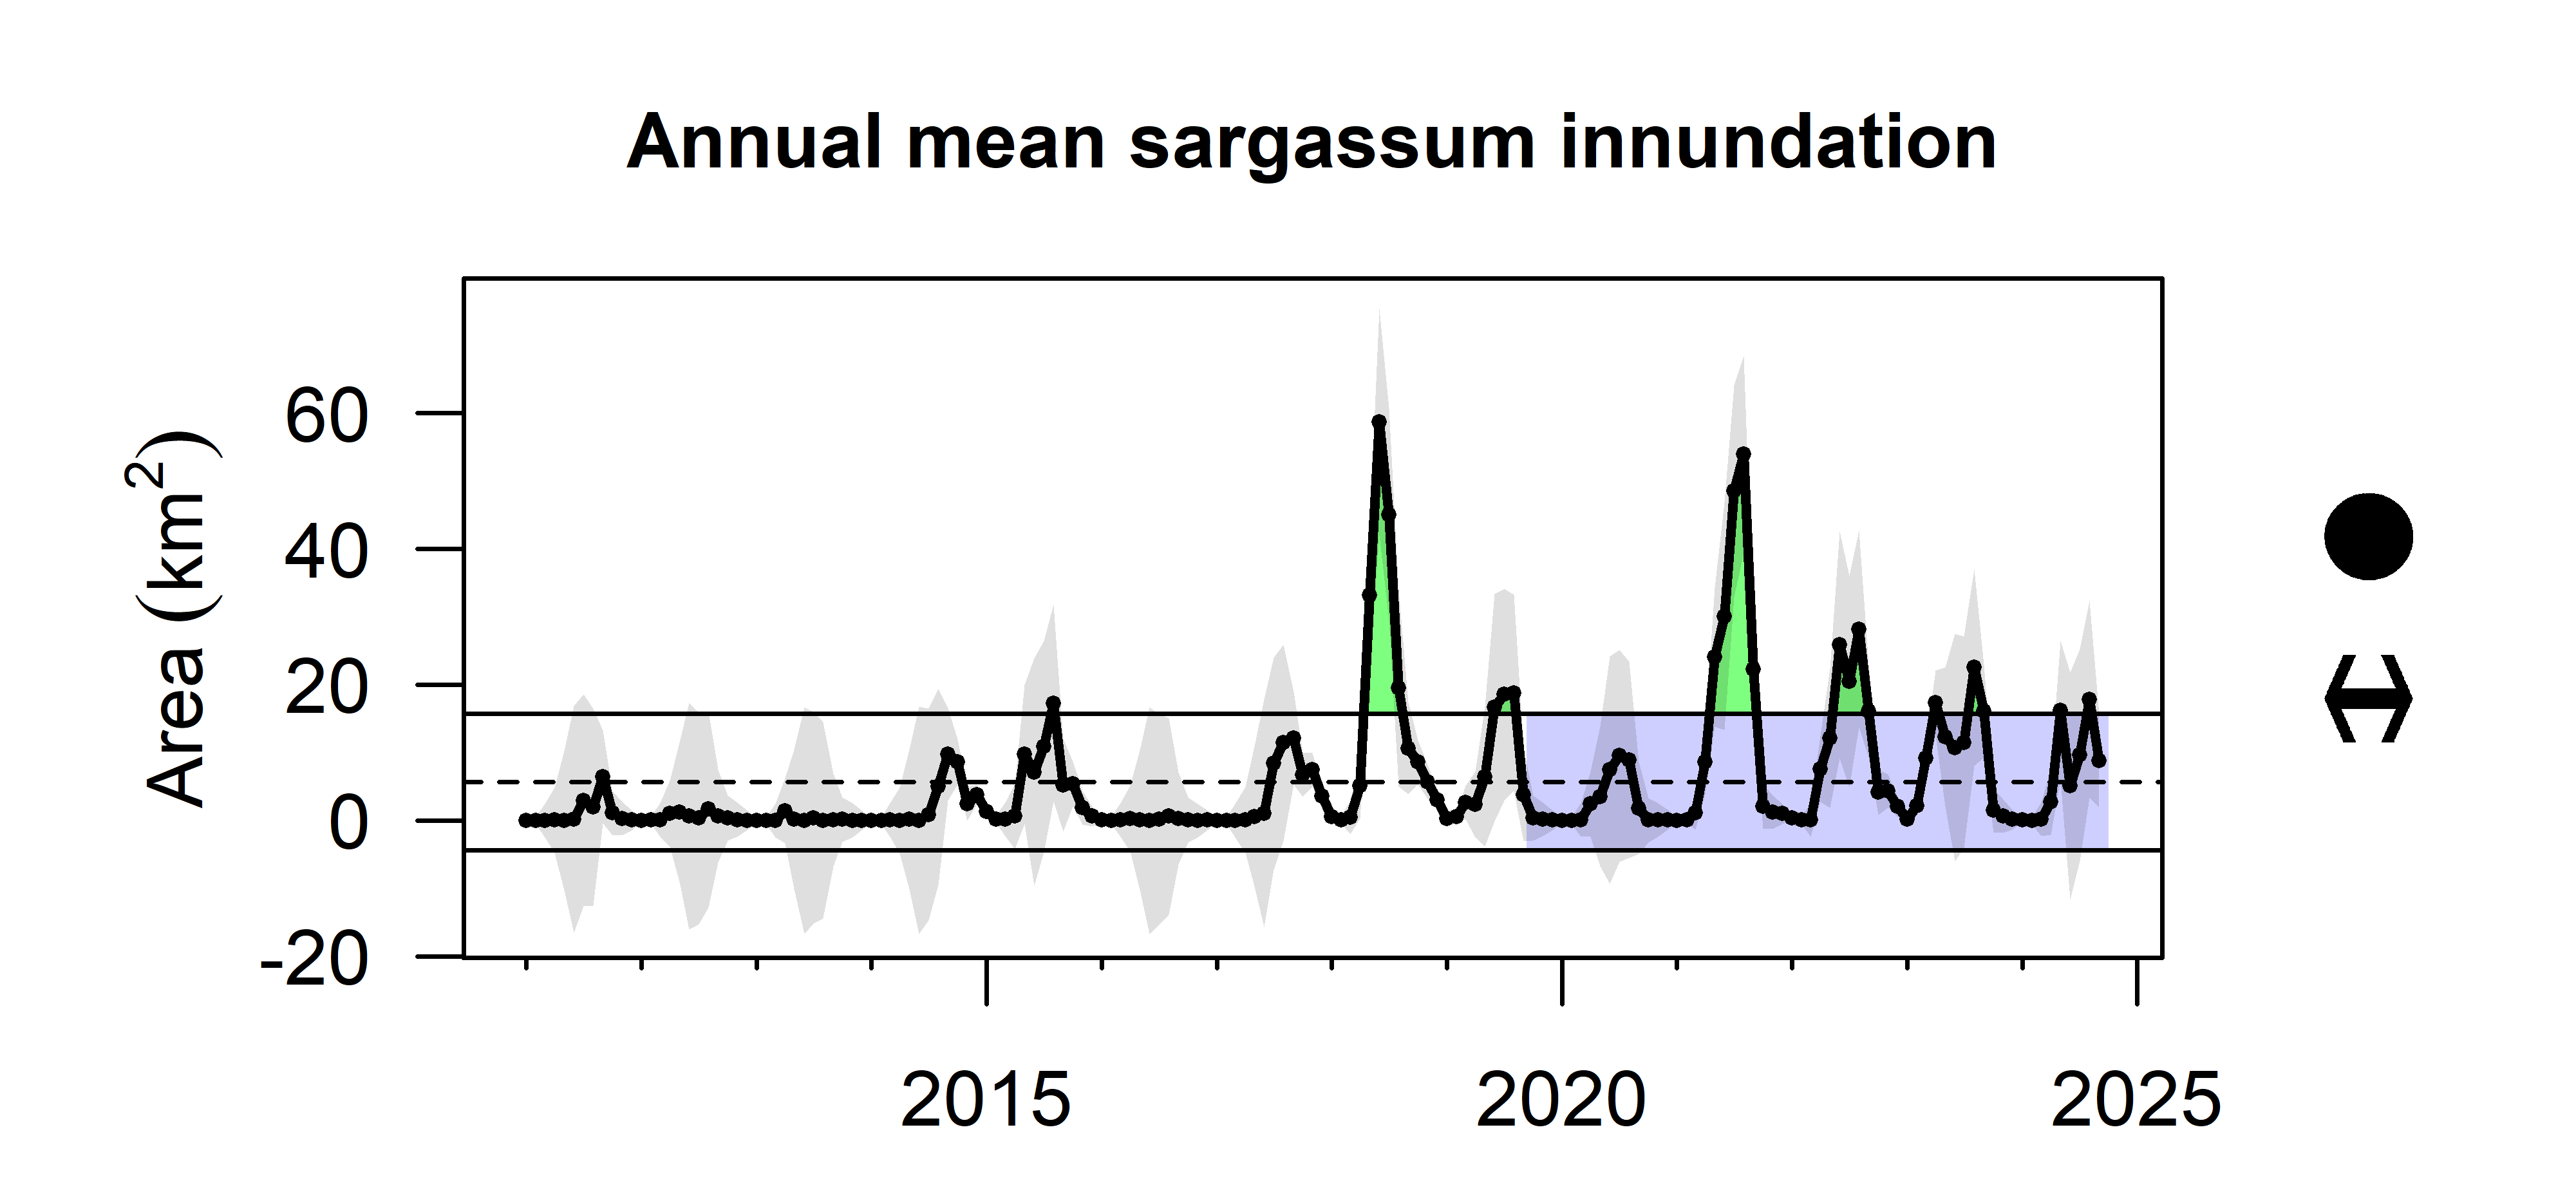
\includegraphics{indicator_plots/Sargassum_plot_final.png}

}

\caption{\label{fig-sarg}Annual mean sargassum inundation in square km
of cover in the U.S. Caribbean.}

\end{figure}%

\section{Market disturbances}\label{market-disturbances}

Alterations to typical fishing patterns can be quantified by analyzing
the seasonality of how fishing activity is distributed throughout the
year and detecting deviations from average patterns. A market
disturbance indicator was developed by calculating the proportion of
landings in each month of the year, and summing the square of deviations
between those monthly proportions from the mean proportions across all
years. In Puerto Rico there is little trend in the indicator; however
there were disturbances in 2005 and 2020-2021. In St.~Thomas, the
indicator increases throughout time and detects a major disturbance in
the 2017-18 fishing season. In St.~Croix, disturbance levels were high
in 2017-18 and also 2019-20 (Figure~\ref{fig-dist}).

\begin{figure}

\centering{

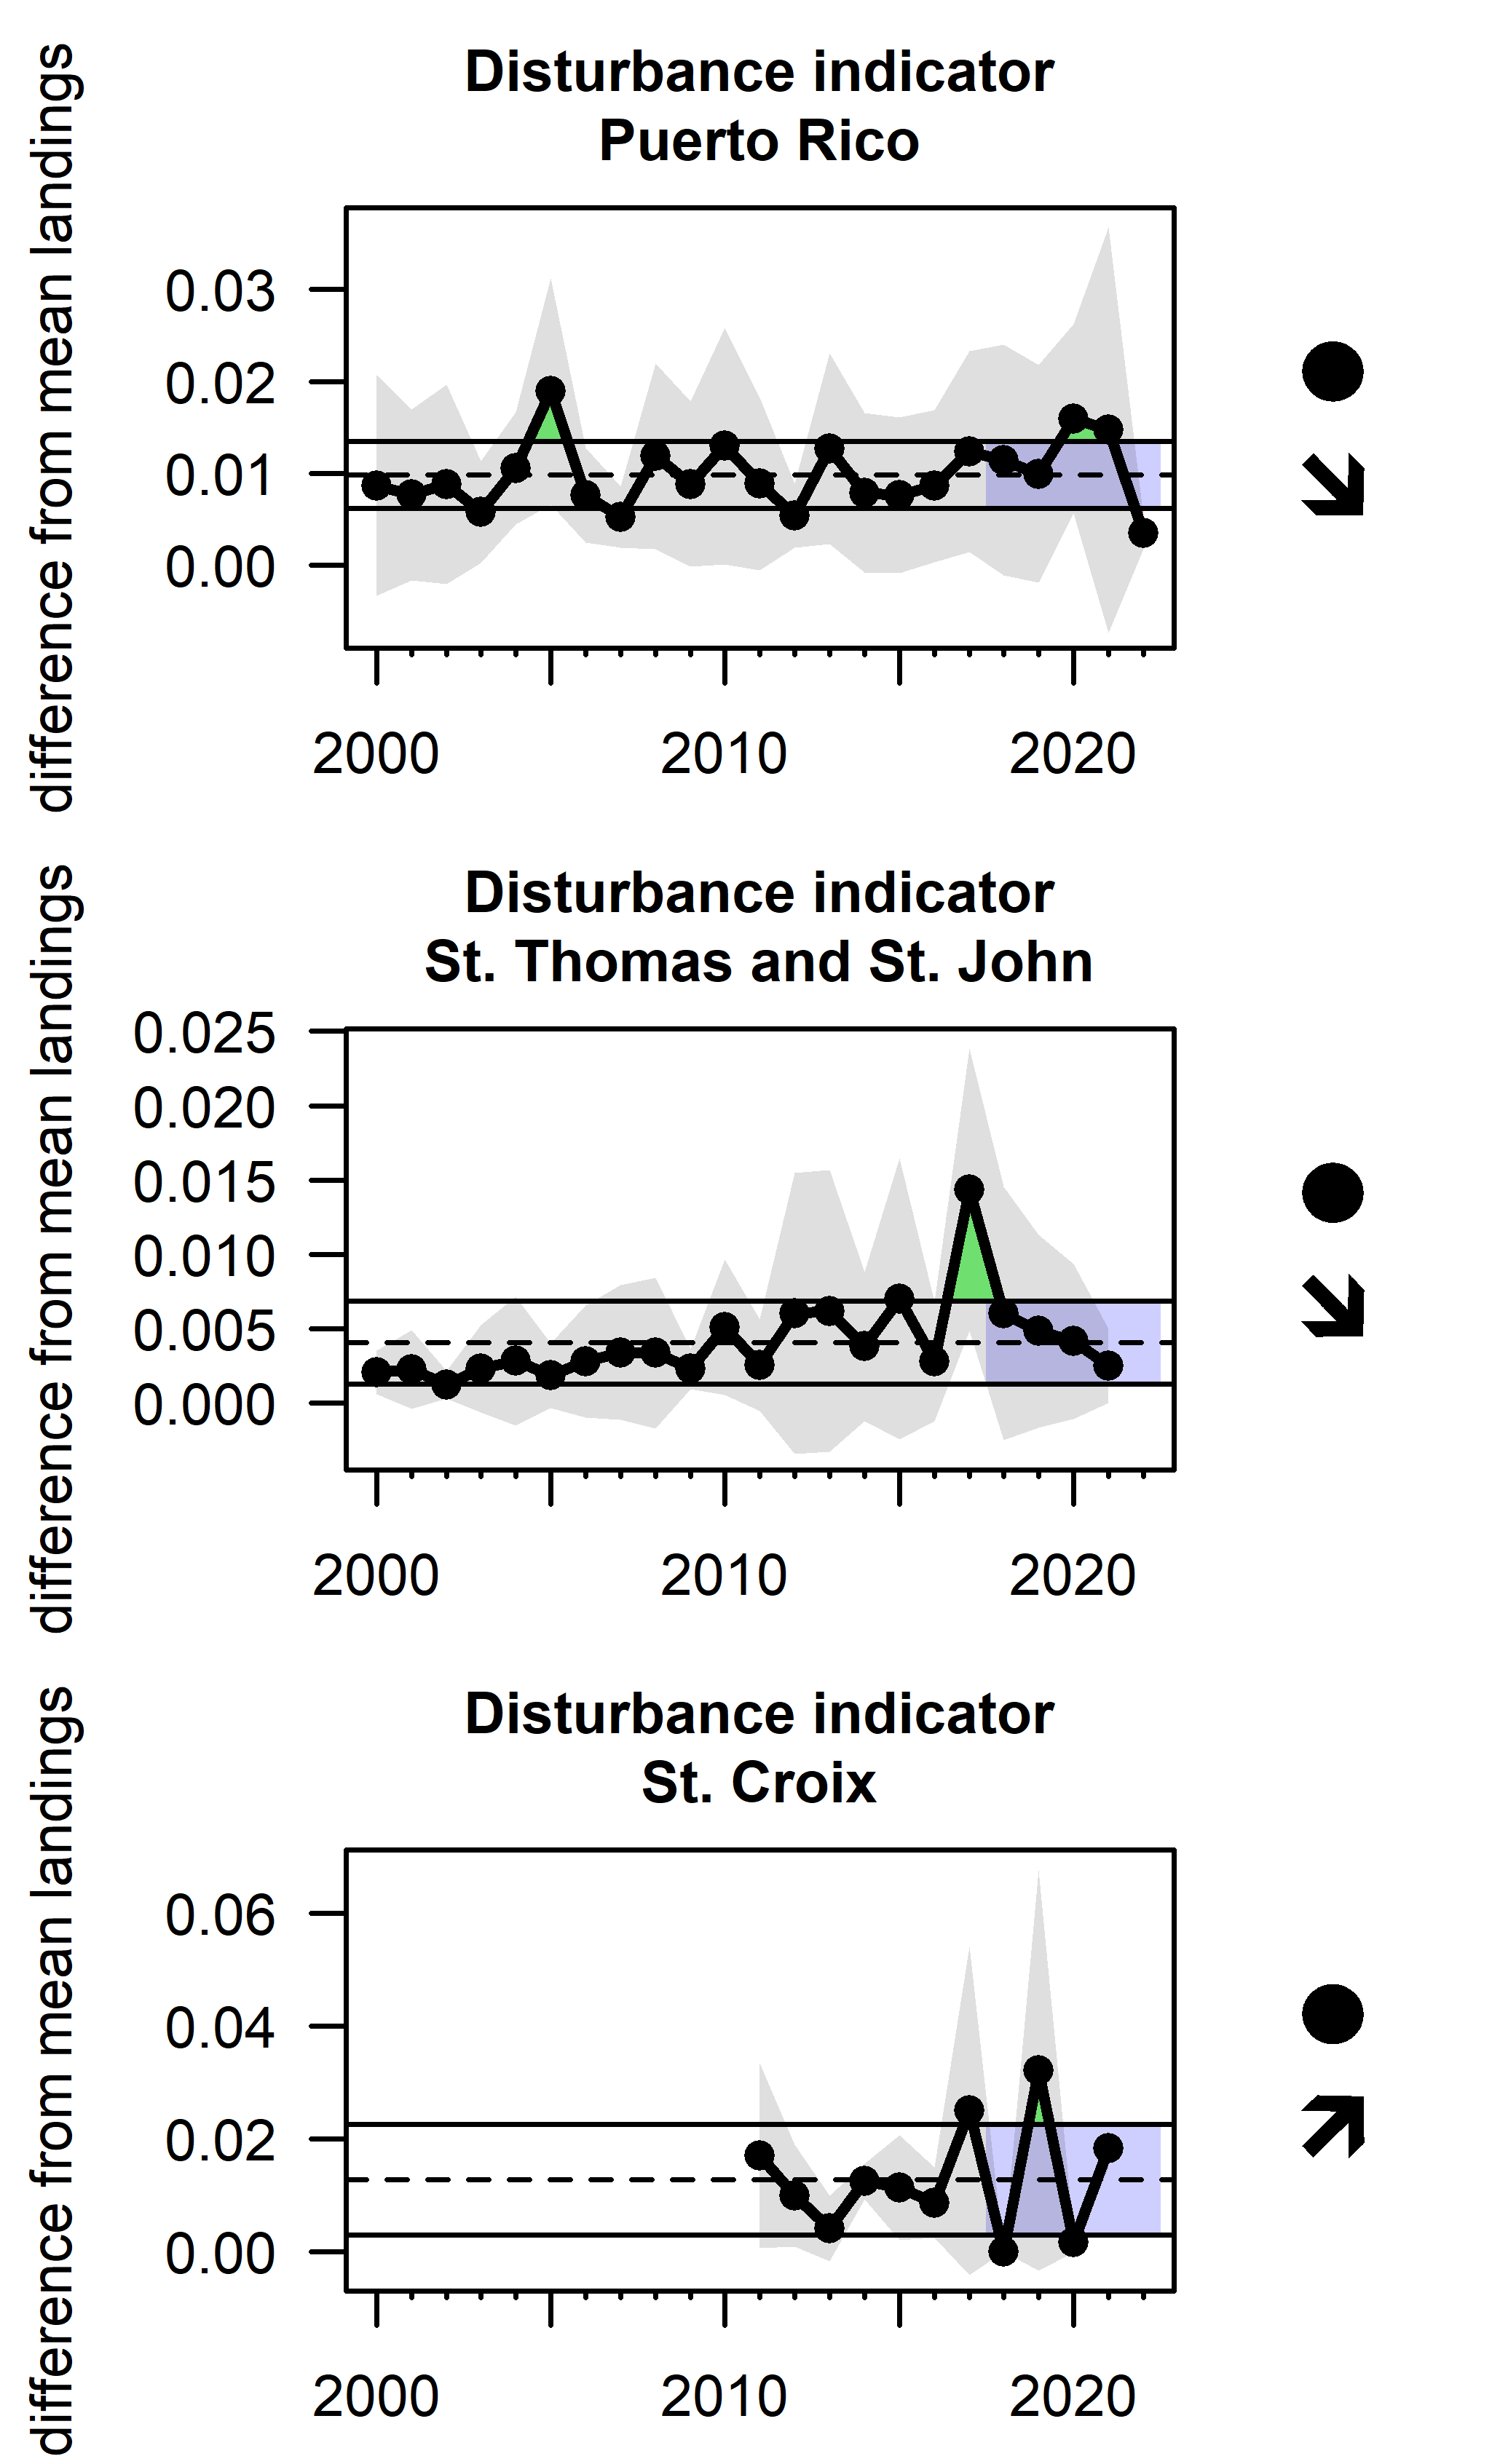
\includegraphics{indicator_plots/disturbance_plot_final.png}

}

\caption{\label{fig-dist}Disturbance level as the difference from mean
landings of top species for the U.S. Caribbean.}

\end{figure}%

\section{Human activity}\label{human-activity}

Human activity has an impact on the marine ecosystem indirectly through
its influence on coastal development and pollution, as well as directly
through marine tourism, fishing and demand for seafood. Human activity
is exerted by the local population as well as the extensive tourism
industry that exists in the U.S. Caribbean. Total population estimates
are reported by the U.S. Census (??) and tourism activity can be
measured through hotel occupancy rates (cite) and the number of air and
cruise passengers (cite). Human population in the U.S. Caribbean has
been declining gradually since 2000 (Figure~\ref{fig-pop}). Tourism has
fluctuated over time, with major decreases in 2017 and 2020
(Figure~\ref{fig-tourist}).

\begin{figure}

\centering{

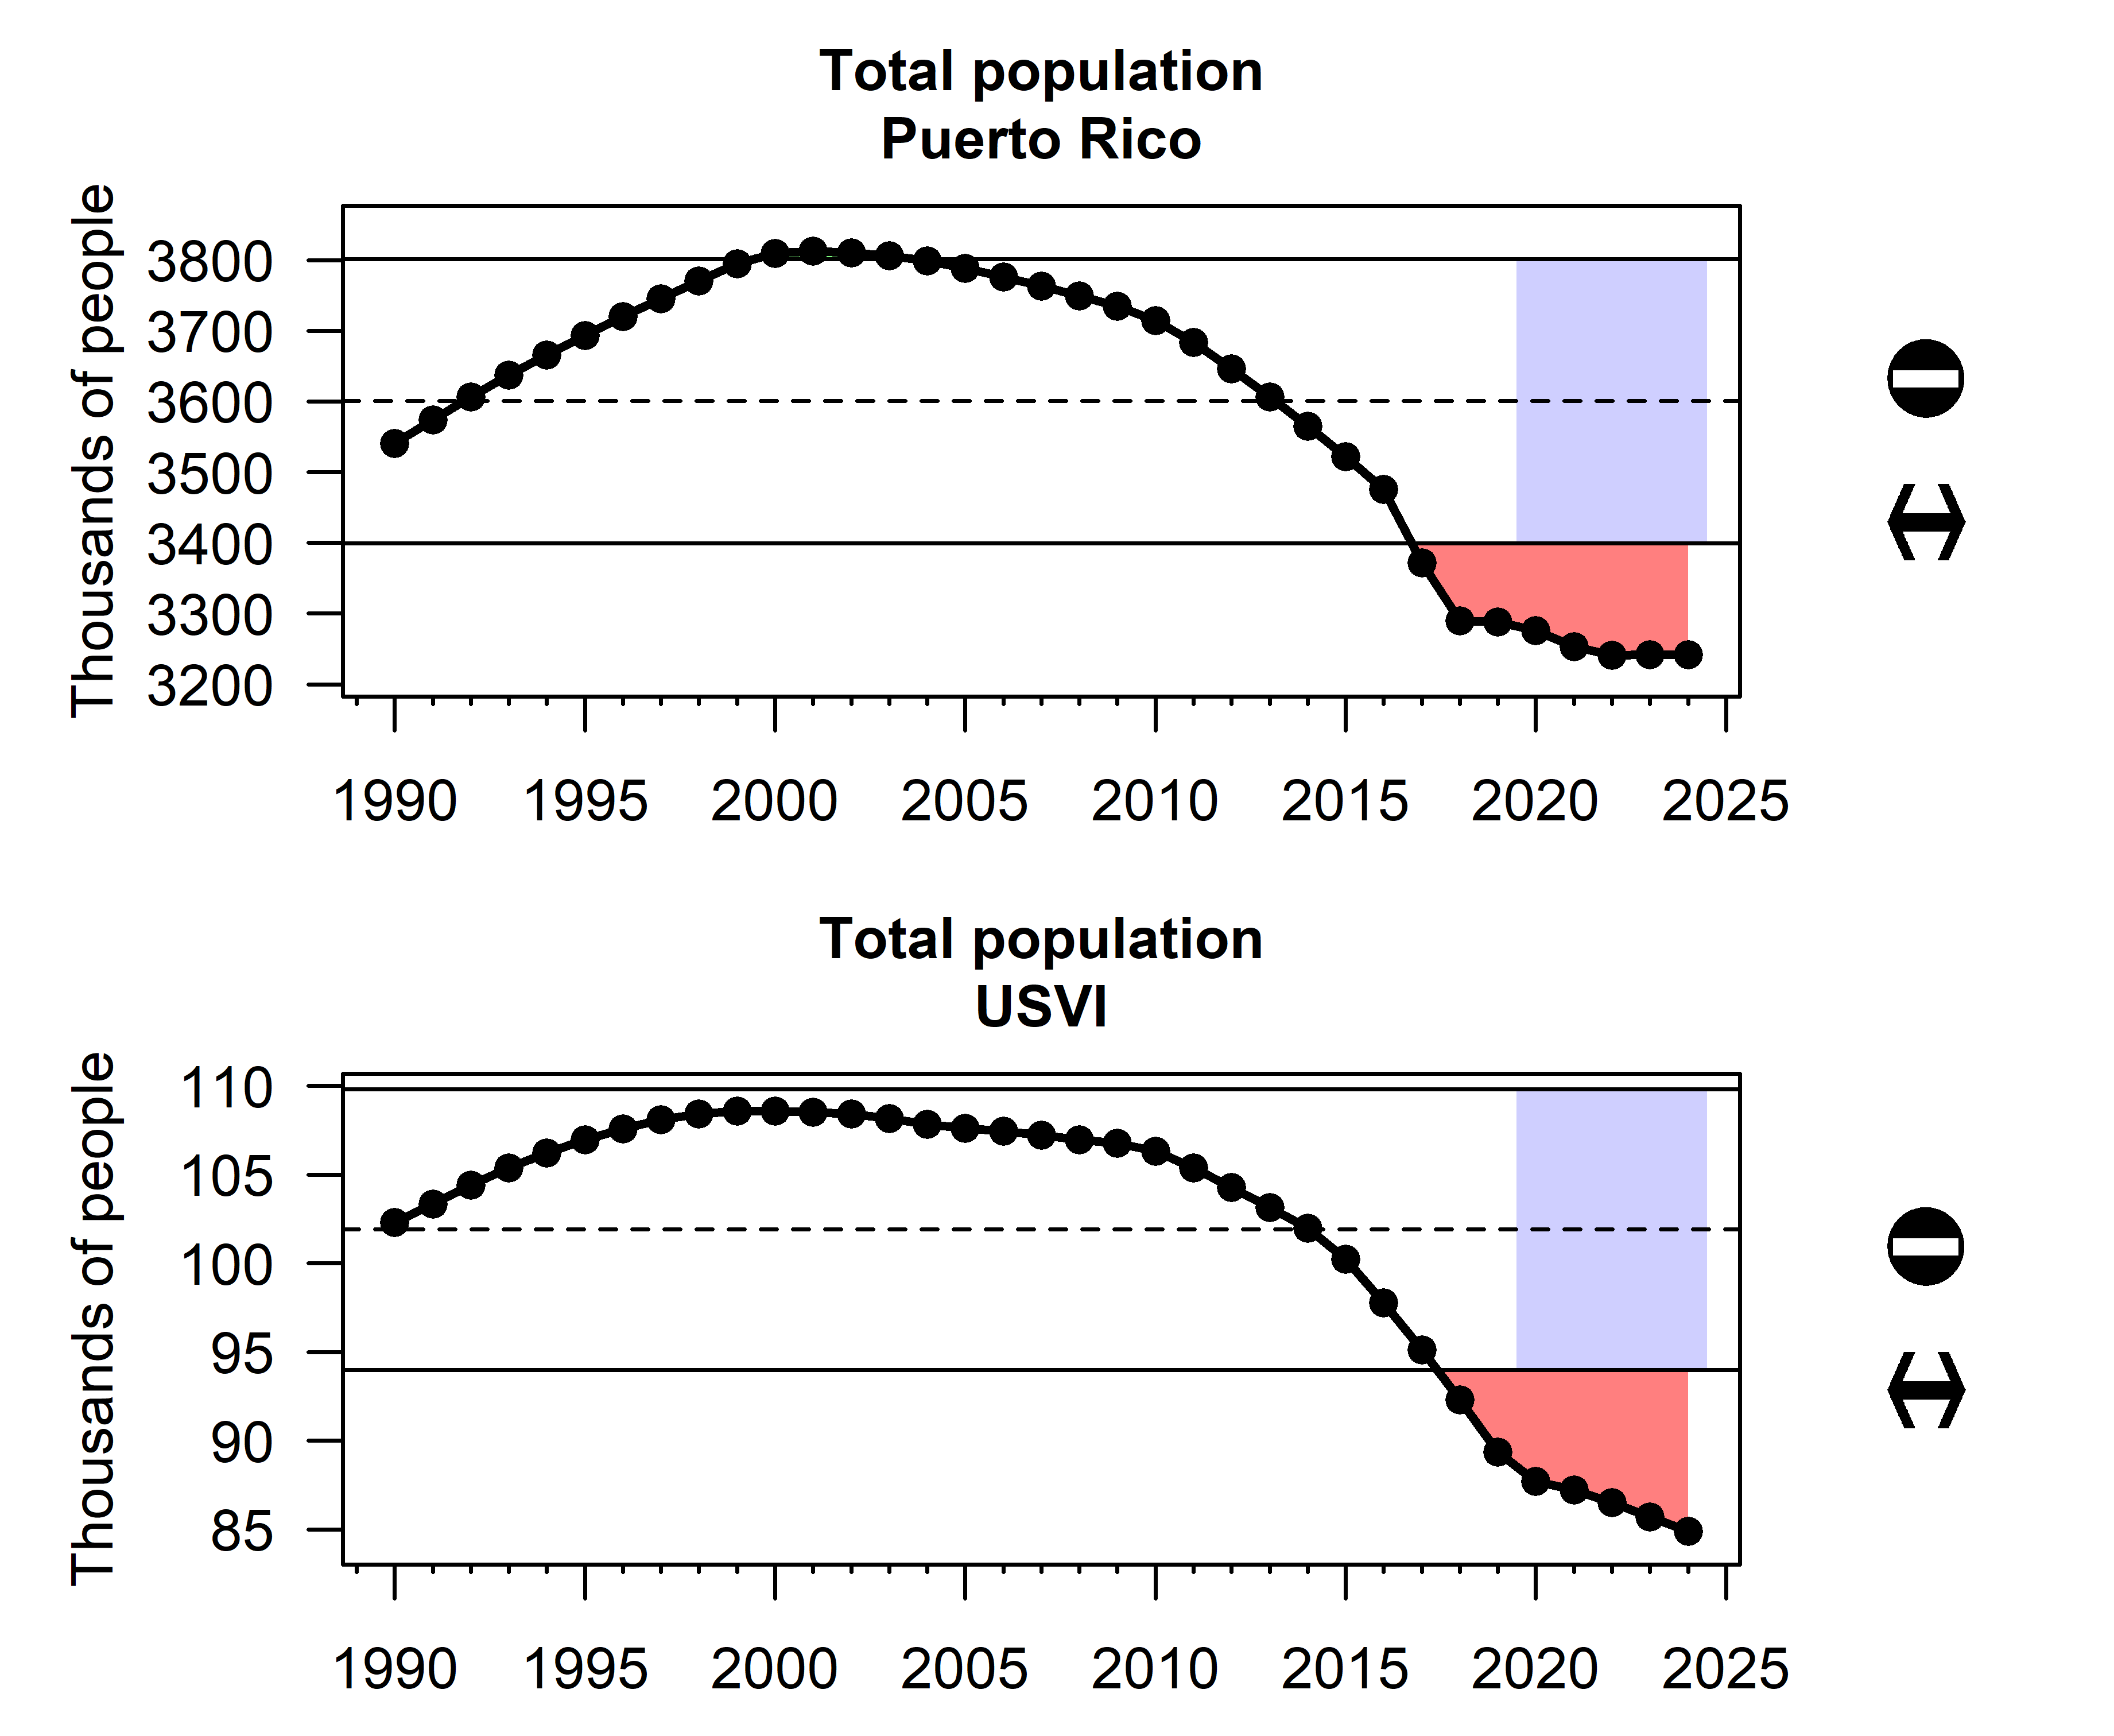
\includegraphics{indicator_plots/population_plot_final.png}

}

\caption{\label{fig-pop}Population change in Puerto Rico and USVI from
2010 through 2024, via census data.}

\end{figure}%

\begin{figure}

\centering{

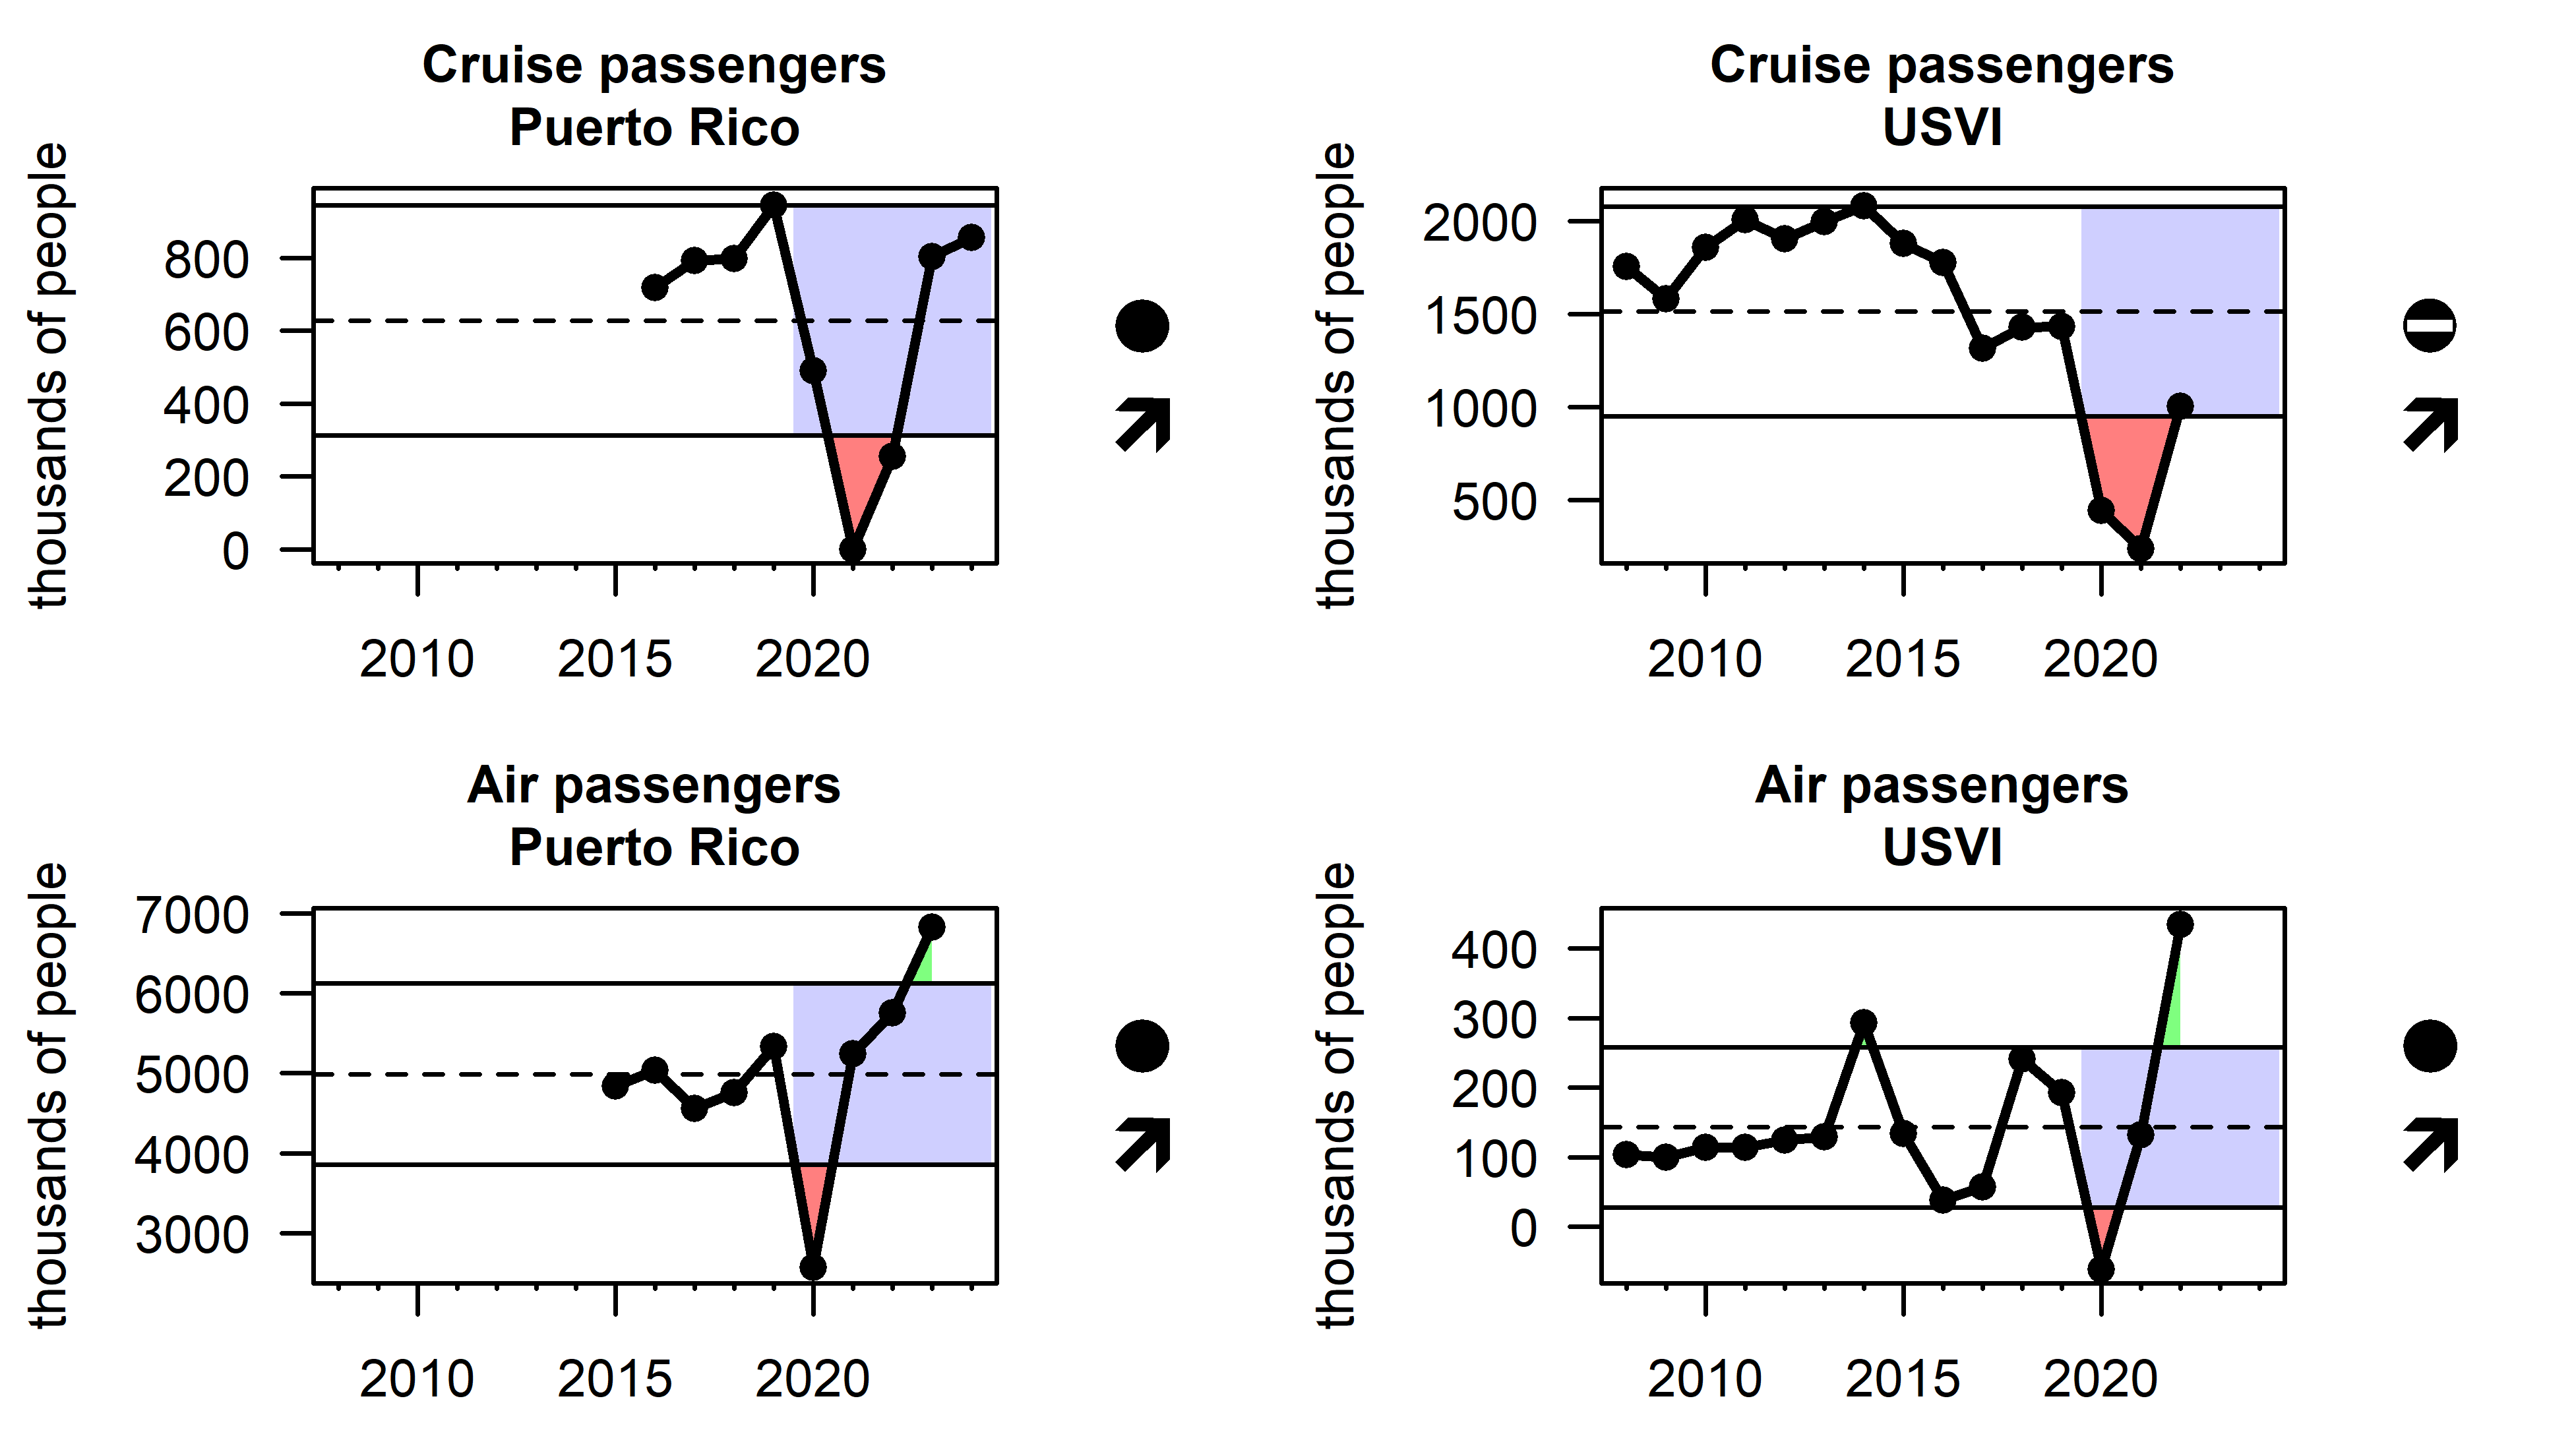
\includegraphics{indicator_plots/cruise_plot_final.png}

}

\caption{\label{fig-tourist}Annual tourism activity in Puerto Rico and
USVI as indicated by the number of cruise and air passengers visiting
the islands.}

\end{figure}%

\bookmarksetup{startatroot}

\chapter{Tracking performance toward fishery management
objectives}\label{tracking-performance-toward-fishery-management-objectives}

In this section, we examine indicators related to broad, ecosystem-level
fishery management objectives.

\section{Food production}\label{food-production}

\subsection{Fishery independent surveys of economically important
species}\label{fishery-independent-surveys-of-economically-important-species}

Fishery-independent surveys are conducted to understand relative
abundance trends in economically important fish species. The Southeast
Fisheries Science Center, in collaboration with many academic and
private partners, has been conducting a visual survey of reef fish
species in the Florida Keys since 1978, and the survey was expanded to
the U.S. Caribbean in 2001 (Smith et al. 2011). Six target fish species
(mutton snapper, yellowtail snapper, red hind, queen triggerfish,
redband parrotfish, and stoplight parrotfish) were selected as key
indicators for the condition of living resources in the U.S. Caribbean,
due to their status as targeted species by recreational and commercial
fishers. Trends in fish density for these species of interest are highly
variable, but density has been at or above the time series average in
recent years for most species. A notable exception is stoplight
parrotfish, which have gradually declined over time in all regions and
density is currently below average in St.~Croix (Figure~\ref{fig-RVCPR},
Figure~\ref{fig-RVCSTSJ}, Figure~\ref{fig-RVCSTX}).

\begin{figure}

\centering{

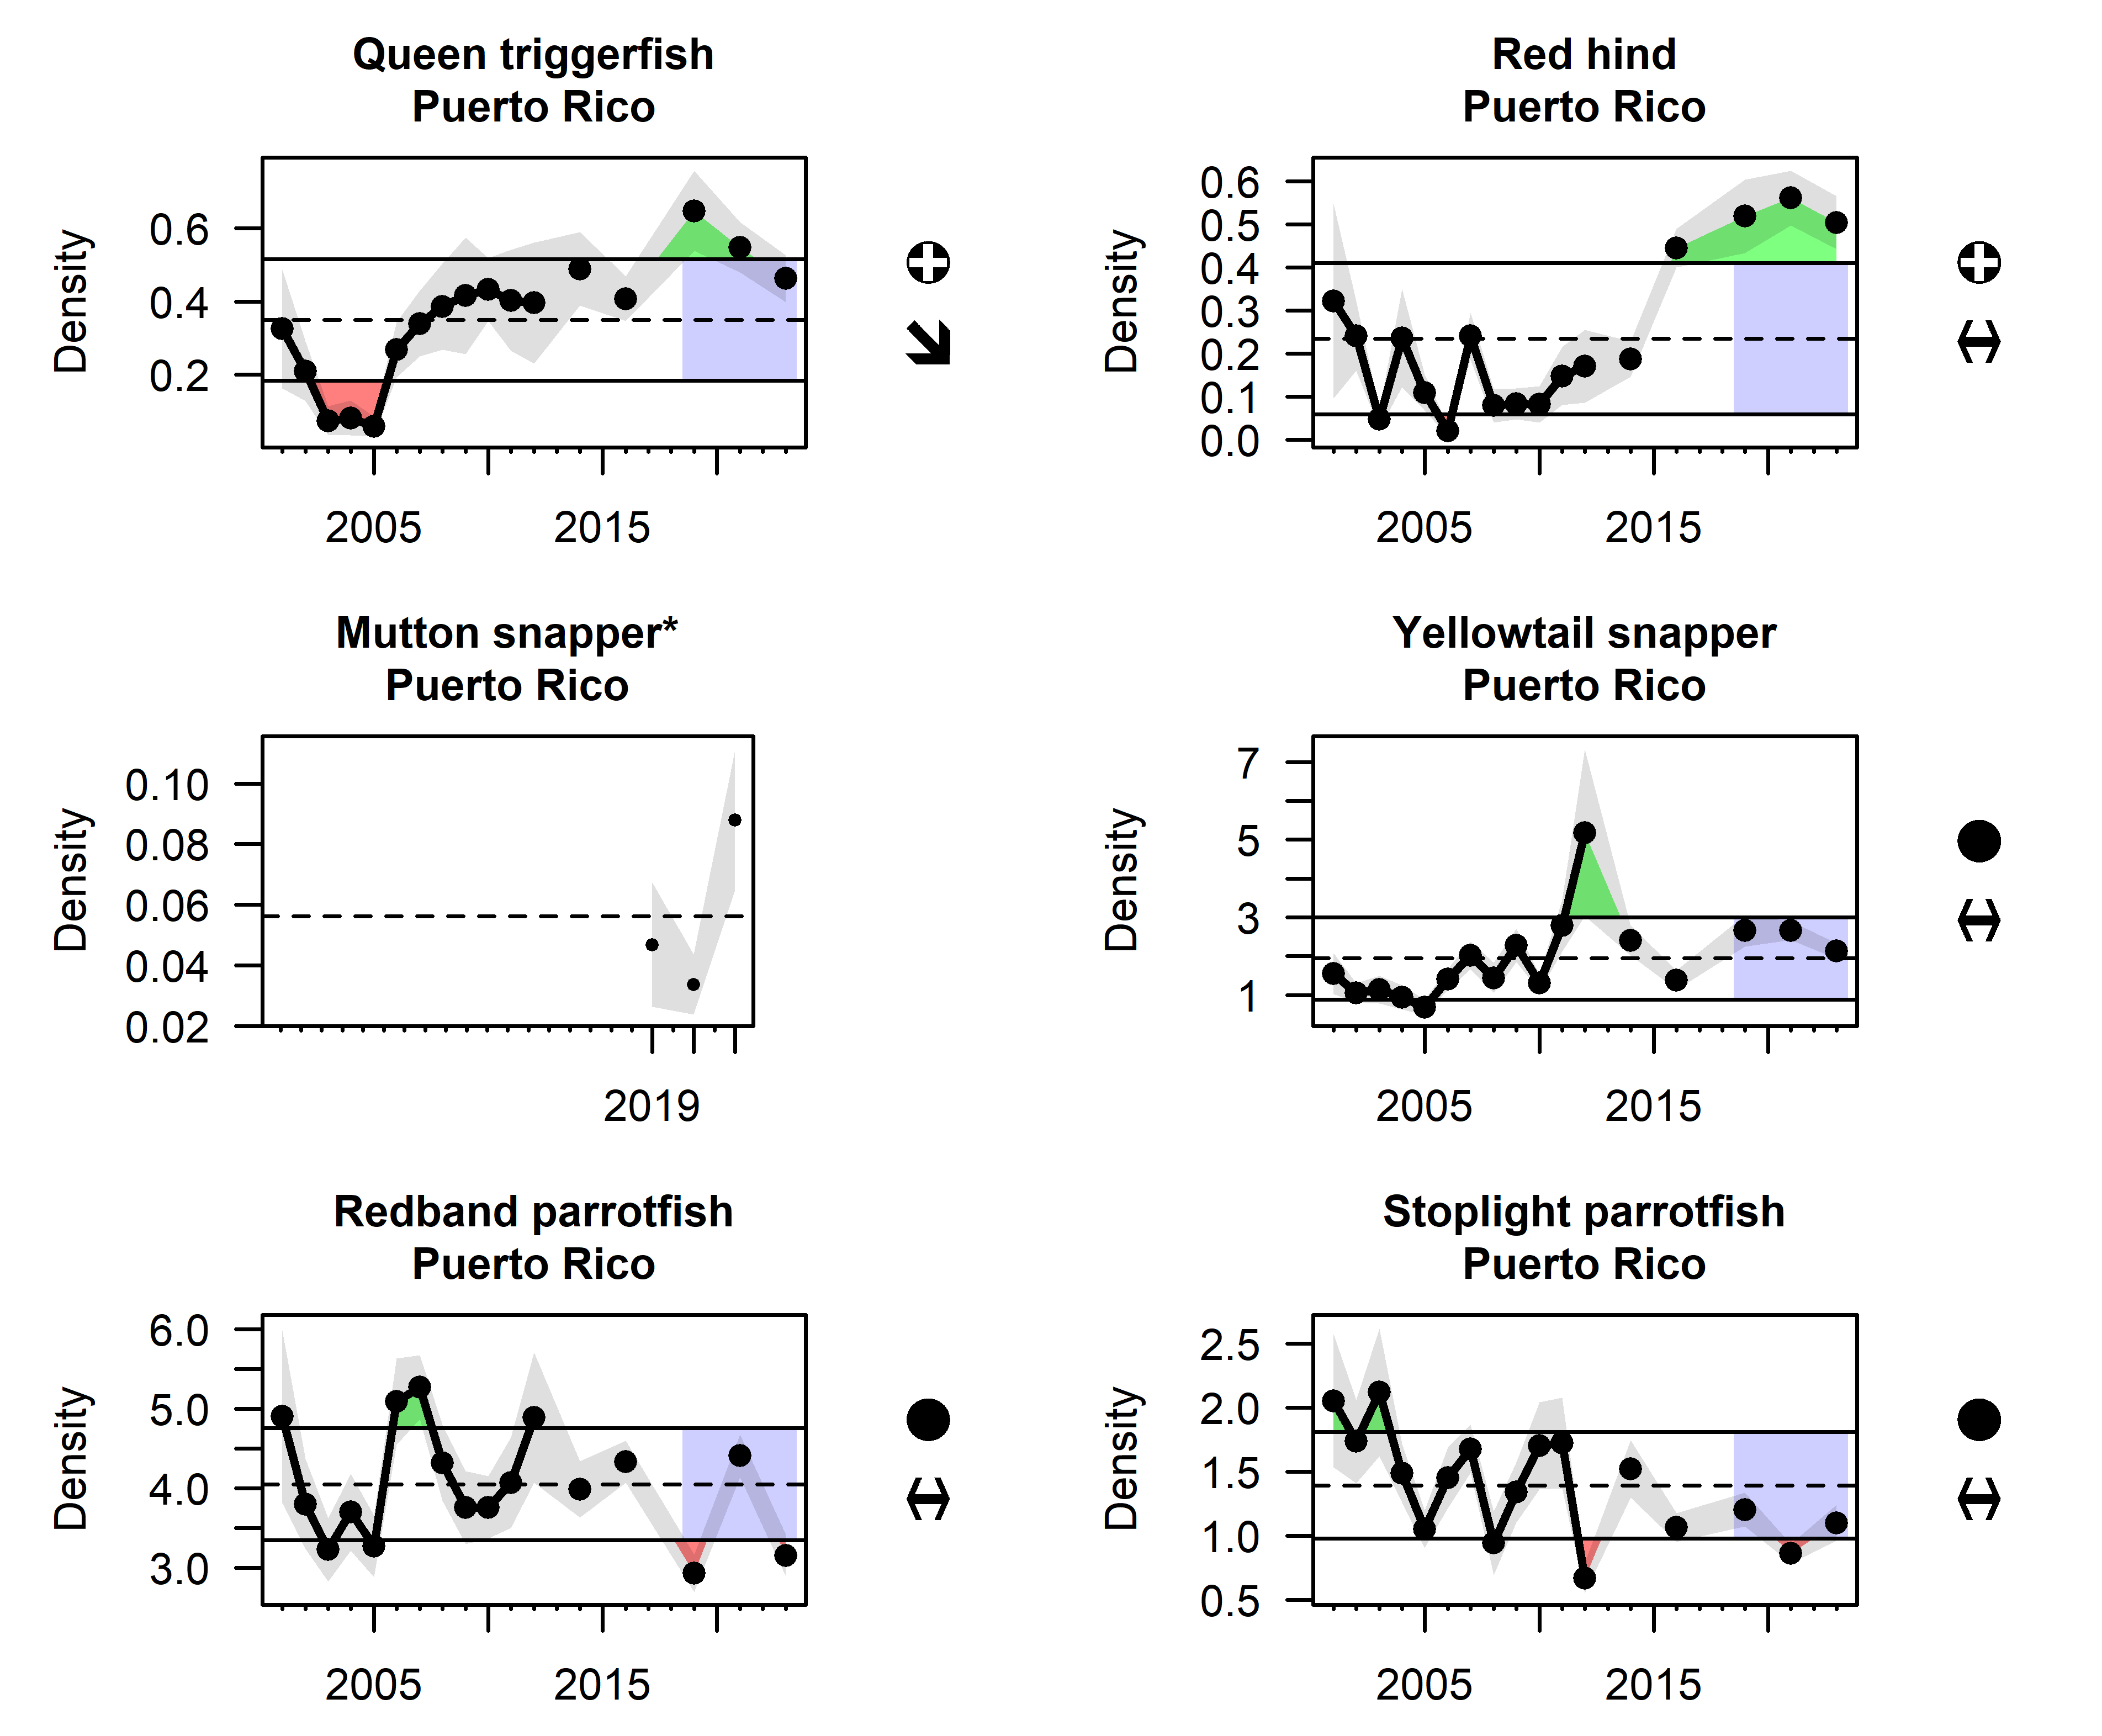
\includegraphics{indicator_plots/RVC_PR_plot_final.png}

}

\caption{\label{fig-RVCPR}Average density of queen triggerfish, red
hind, mutton snapper, yellowtail snapper, redband parrotfish, and
stoplight parrotfish over time in Puerto Rico from the National Coral
Reef Monitoring Program Reef Visual Census data. A change in sampling
methodology occured in 2019, and at the time of publication the mutton
snapper time series had not been calibrated, so data are only available
from 2019 onward.}

\end{figure}%

\begin{figure}

\centering{

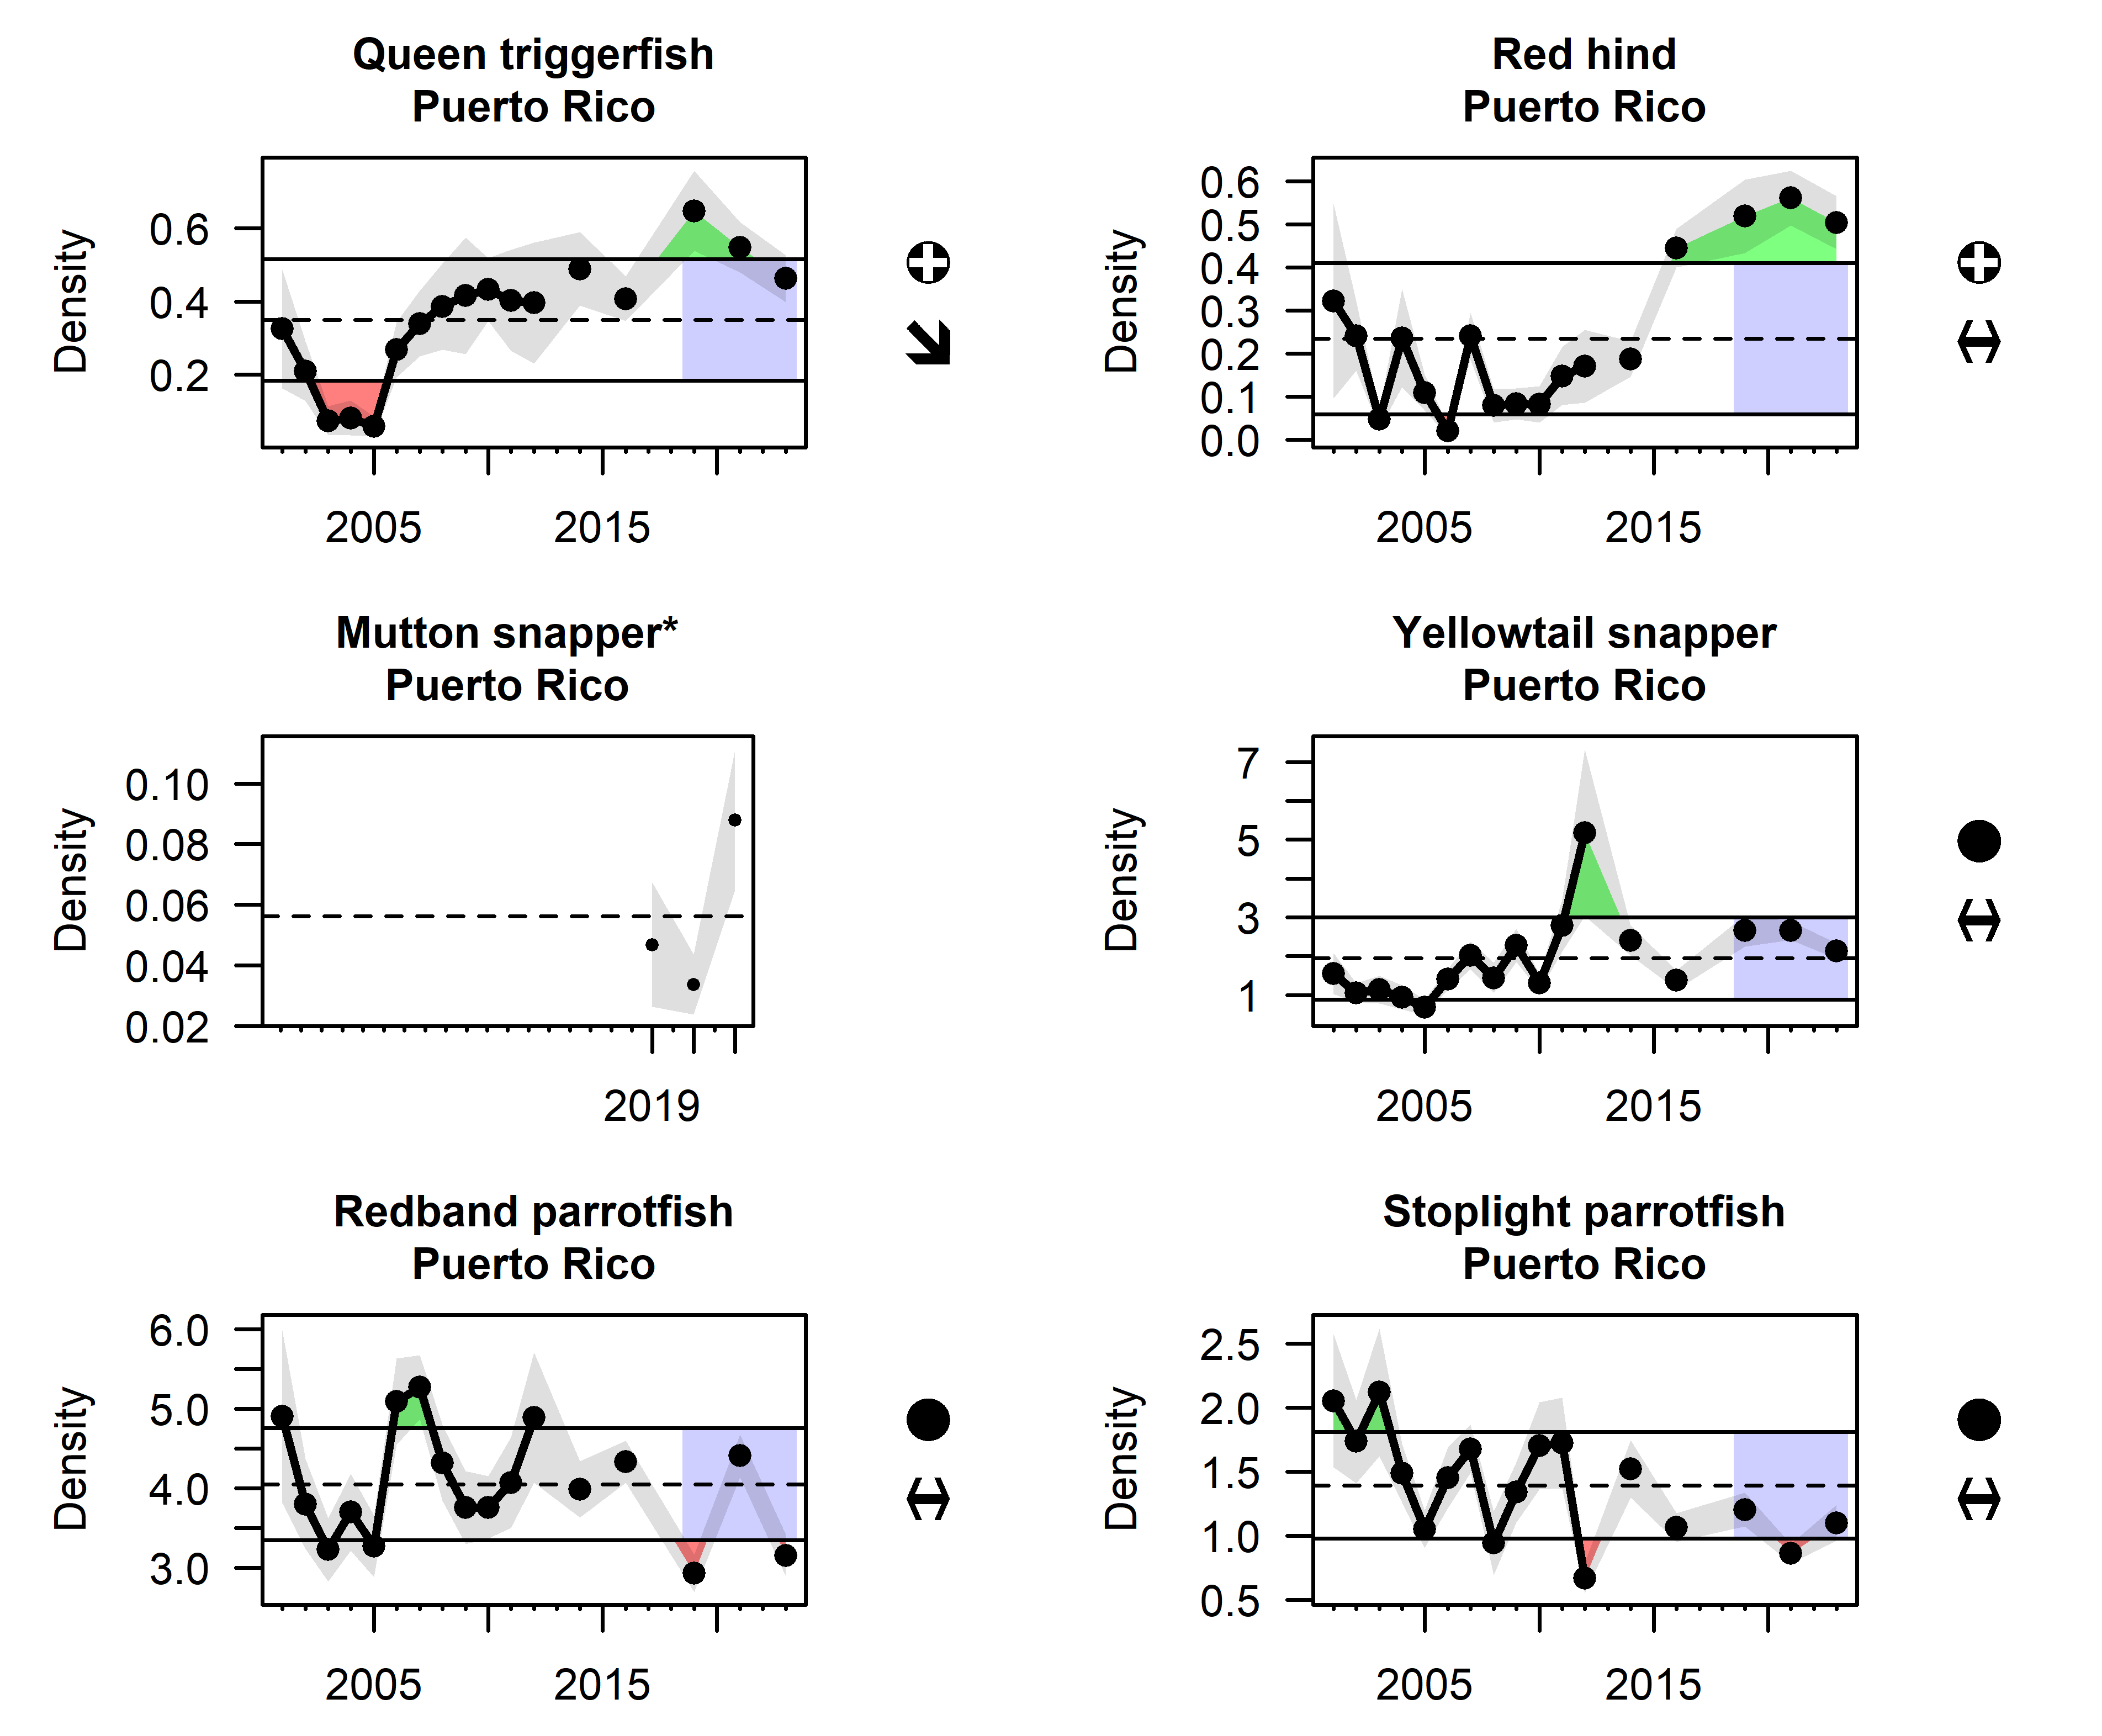
\includegraphics{indicator_plots/RVC_PR_plot_final.png}

}

\caption{\label{fig-RVCSTSJ}Average density of queen triggerfish, red
hind, mutton snapper, yellowtail snapper, redband parrotfish, and
stoplight parrotfish over time in St.~Thomas and St.~John from the
National Coral Reef Monitoring Program Reef Visual Census data. A change
in sampling methodology occured in 2019, and at the time of publication
the mutton snapper time series had not been calibrated, so data are only
available from 2019 onward.}

\end{figure}%

\begin{figure}

\centering{

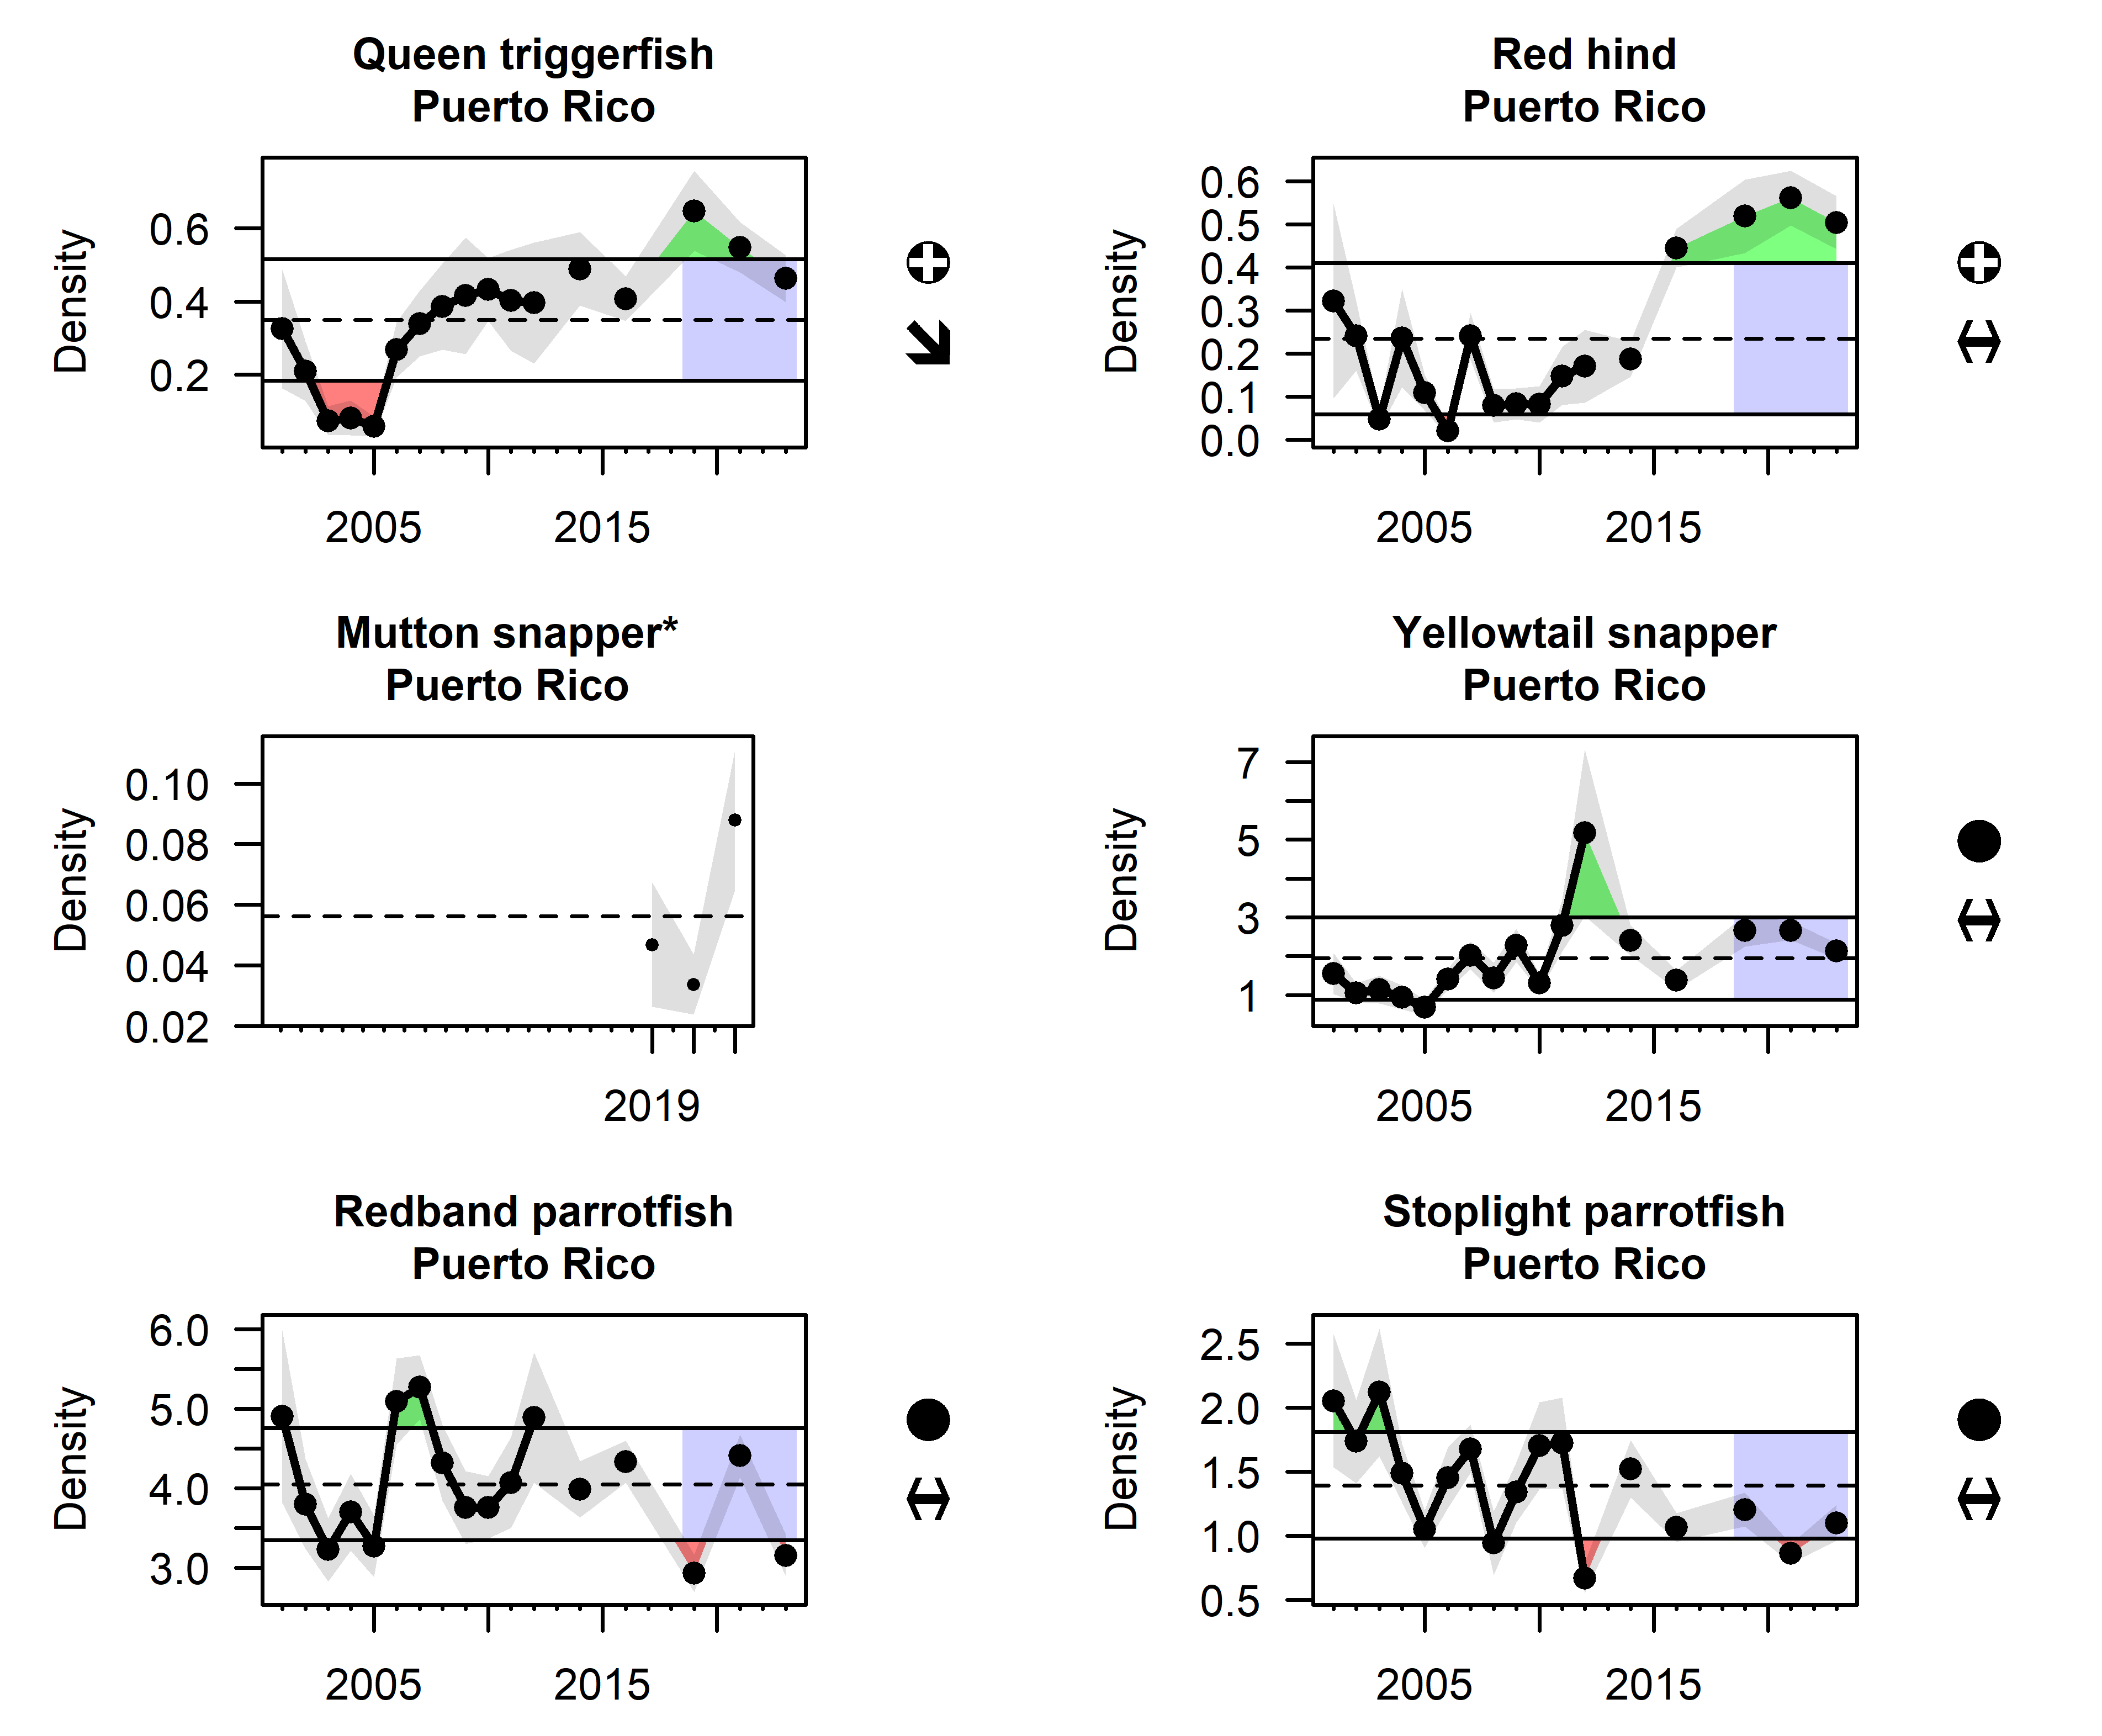
\includegraphics{indicator_plots/RVC_PR_plot_final.png}

}

\caption{\label{fig-RVCSTX}Average density of queen triggerfish, red
hind, mutton snapper, yellowtail snapper, redband parrotfish, and
stoplight parrotfish over time in St.~Croix from the National Coral Reef
Monitoring Program Reef Visual Census data. A change in sampling
methodology occured in 2019, and at the time of publication the mutton
snapper time series had not been calibrated, so data are only available
from 2019 onward.}

\end{figure}%

Fishery-independent surveys can be used to look at changes in the
overall fish community and understand processes affecting multiple
suites of species. The Puerto Rico Long-Term Coral Reef Monitoring
Program (PRCRMP) has conducted annual surveys of fish and benthic
organisms since 1999 (Natural and Environmental Resources 2019).
Similarly, the Territorial Coral Reef Monitoring Program (TCRMP)
conducts annual to semi-annual surveys of coral health, fish community
structure and coral health (cite). Commercial fish density is calculated
by taking the average number of commercial fish per transect over time.
The slope of the size spectrum is calculated by binning all observed
commercial fish lengths into size categories and then fitting a linear
regression through the log-transformed histogram; a more negative slope
represents relatively fewer large fish and potentially increased fishing
impacts. In Puerto Rico, average commercial fish density was noisy but
stable over time; insufficient data were available with which to
estimate the slope of the size spectra. In the USVI, commercial fish
density was stable over time with a large peak in 2011; the slope of the
size spectrum was also relatively stable with a sudden decrease in 2011.
Together these indicators convey the sudden appearance of many small
species, suggestive of a large recruitment event across multiple species
(Figure~\ref{fig-fishdensity}).

\begin{figure}

\centering{

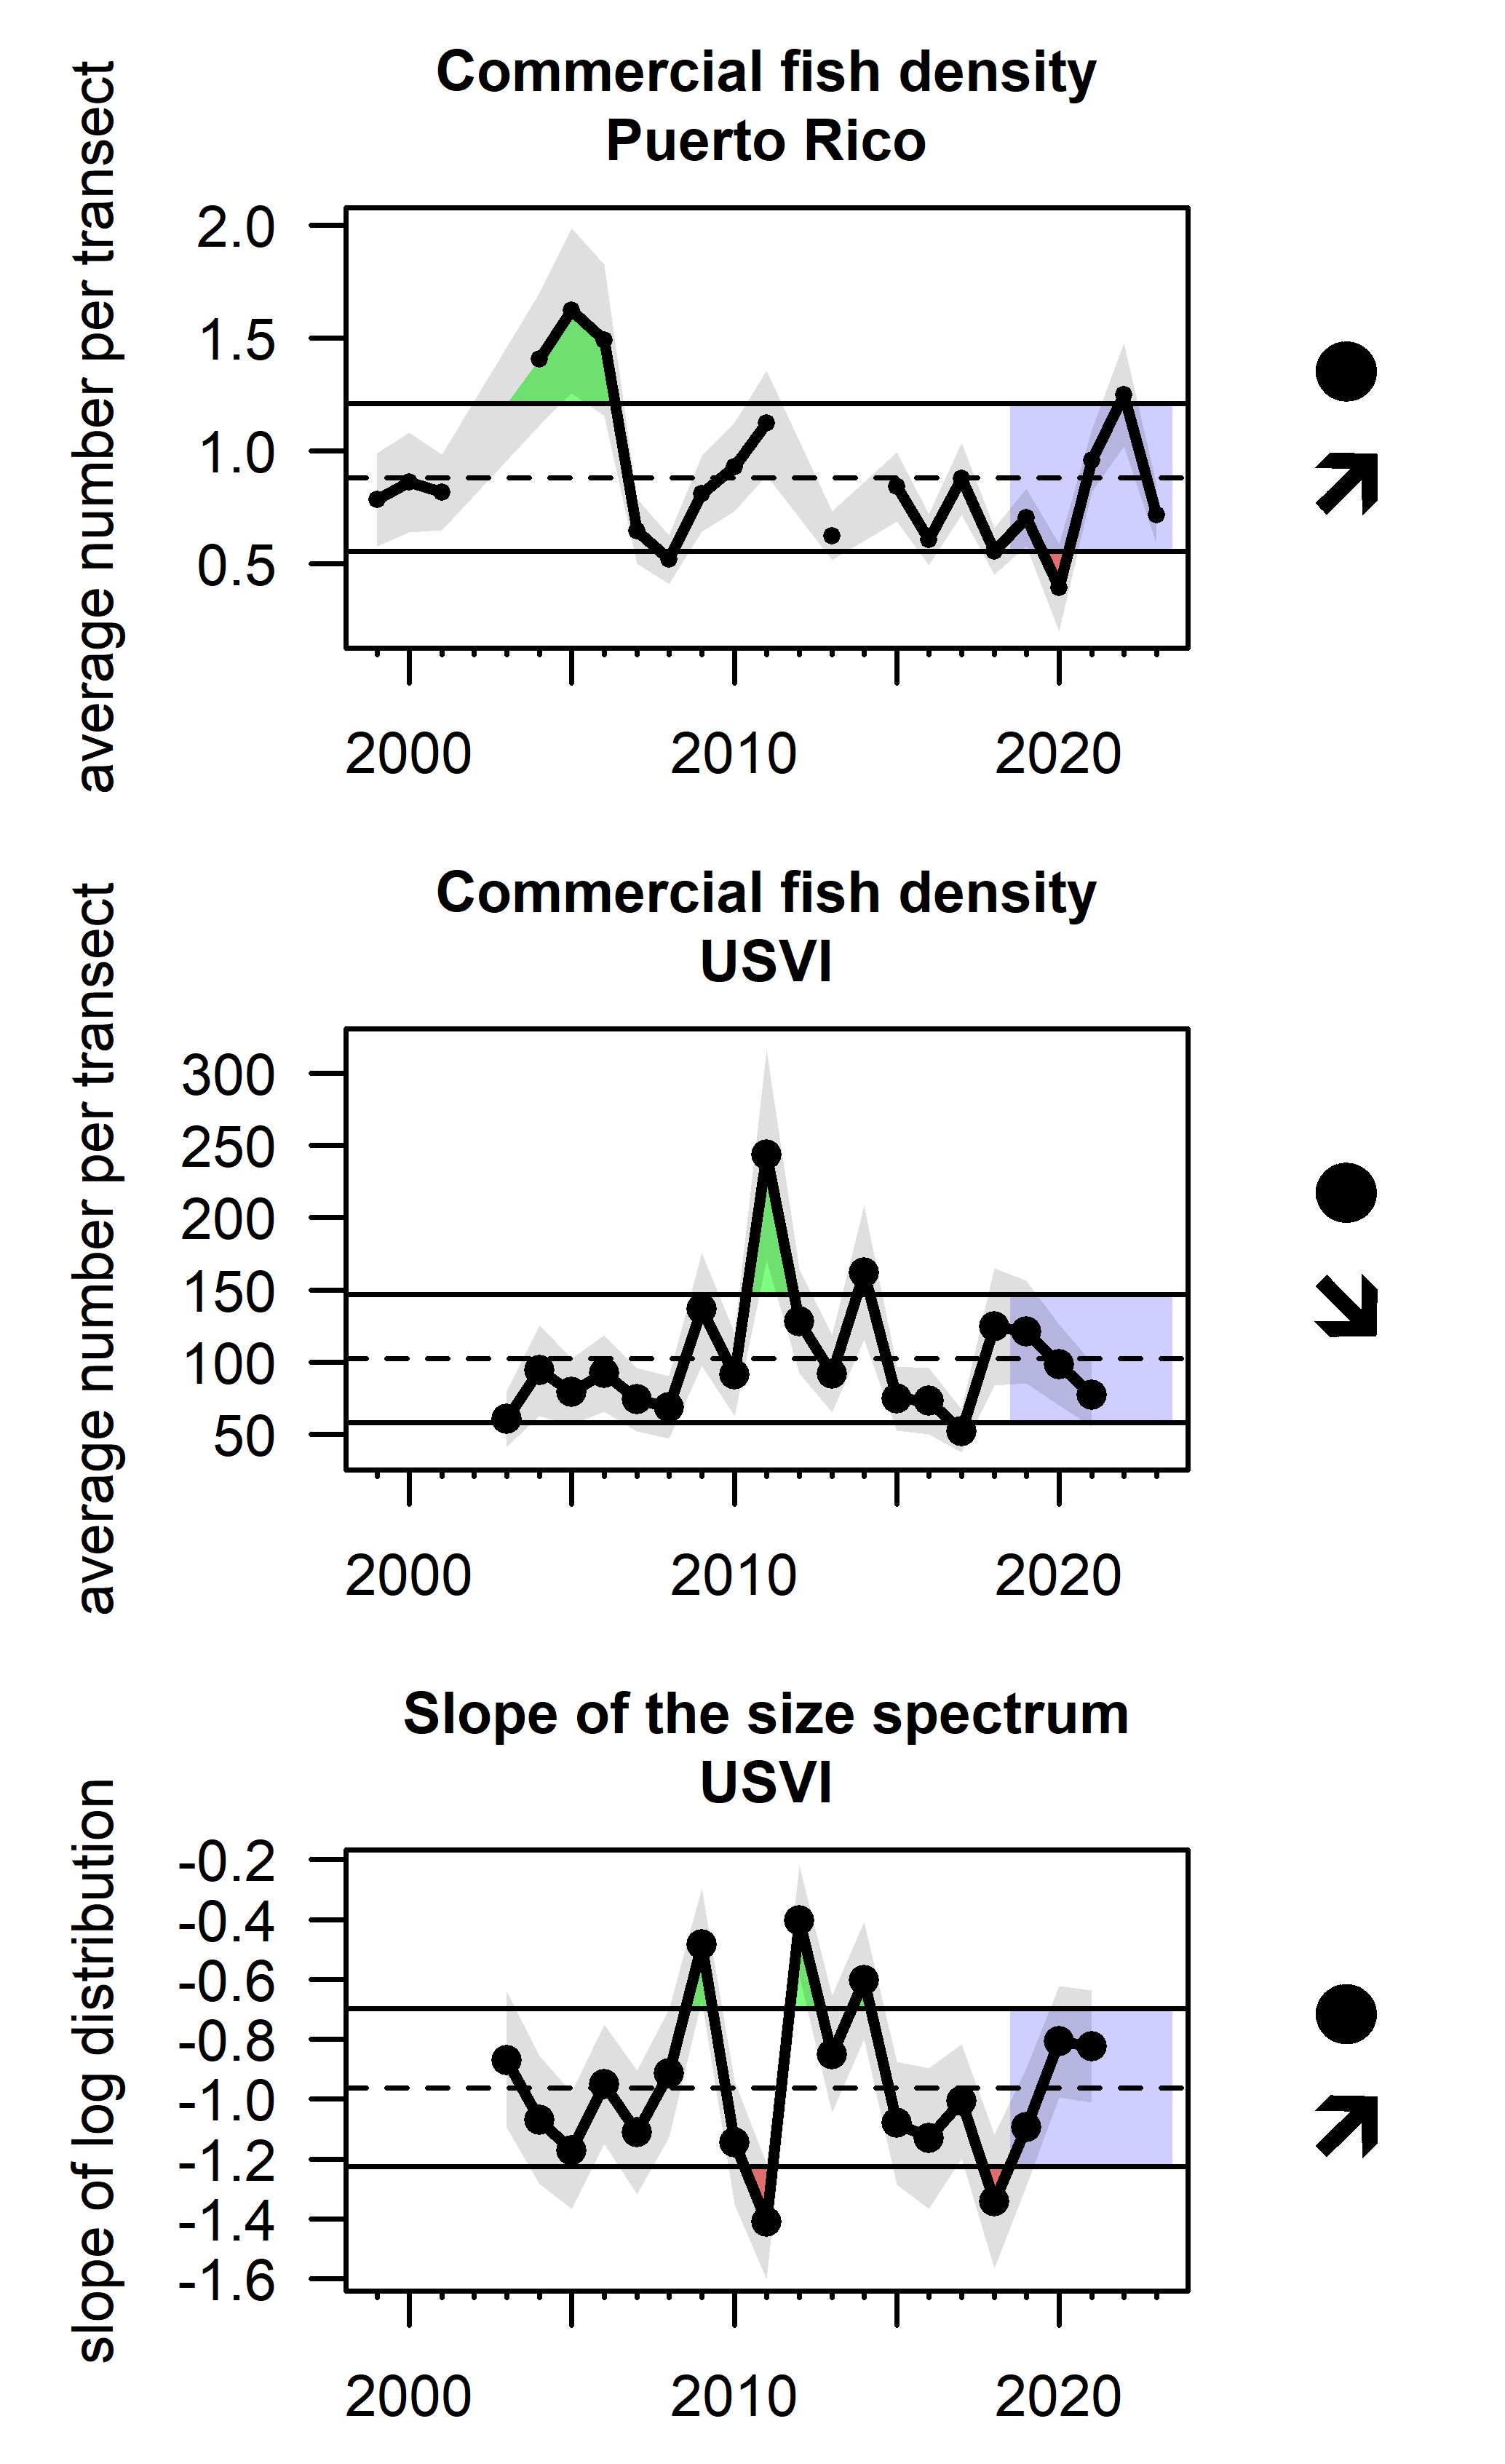
\includegraphics{indicator_plots/fish_density_plot_final.png}

}

\caption{\label{fig-fishdensity}fish density}

\end{figure}%

\subsection{Pelagic:demersal ratio}\label{pelagicdemersal-ratio}

The ratio of pelagic to demersal species is thought to be responsive to
nutrient inputs and the quality of benthic habitat in marine ecosystems
(Leiva Moreno et al. 2000); in the context of small islands in the
tropical seas, it conveys the availability and productivity of pelagic
habitats relative to the size of the shelf and productivity of coral
reef habitats. Ratios of pelagic to demersal catch were calculated based
on total pounds reported in the Caribbean Commercial Landings data,
following a classification of all species based on their reported
ecology in FishBase (Froese and Pauly 2024). In St.~Croix, the
pelagic-demersal ratio is much higher than the other islands, due to the
small shelf area and limited availability of reef habitat; interannual
fluctuations for this island are largely influenced by landings of
dolphinfish and tunas. In Puerto Rico, the pelagic-demersal ratio has
increased in recent years; this may be due to changes in reporting
(logbook to e-reporting). In St.~Thomas and St.~John, the ratio has
gradually increased over time; the large peak in 2018 could have been a
result of hurricane-induced reef habitat loss (Figure~\ref{fig-PD}).

\begin{figure}

\centering{

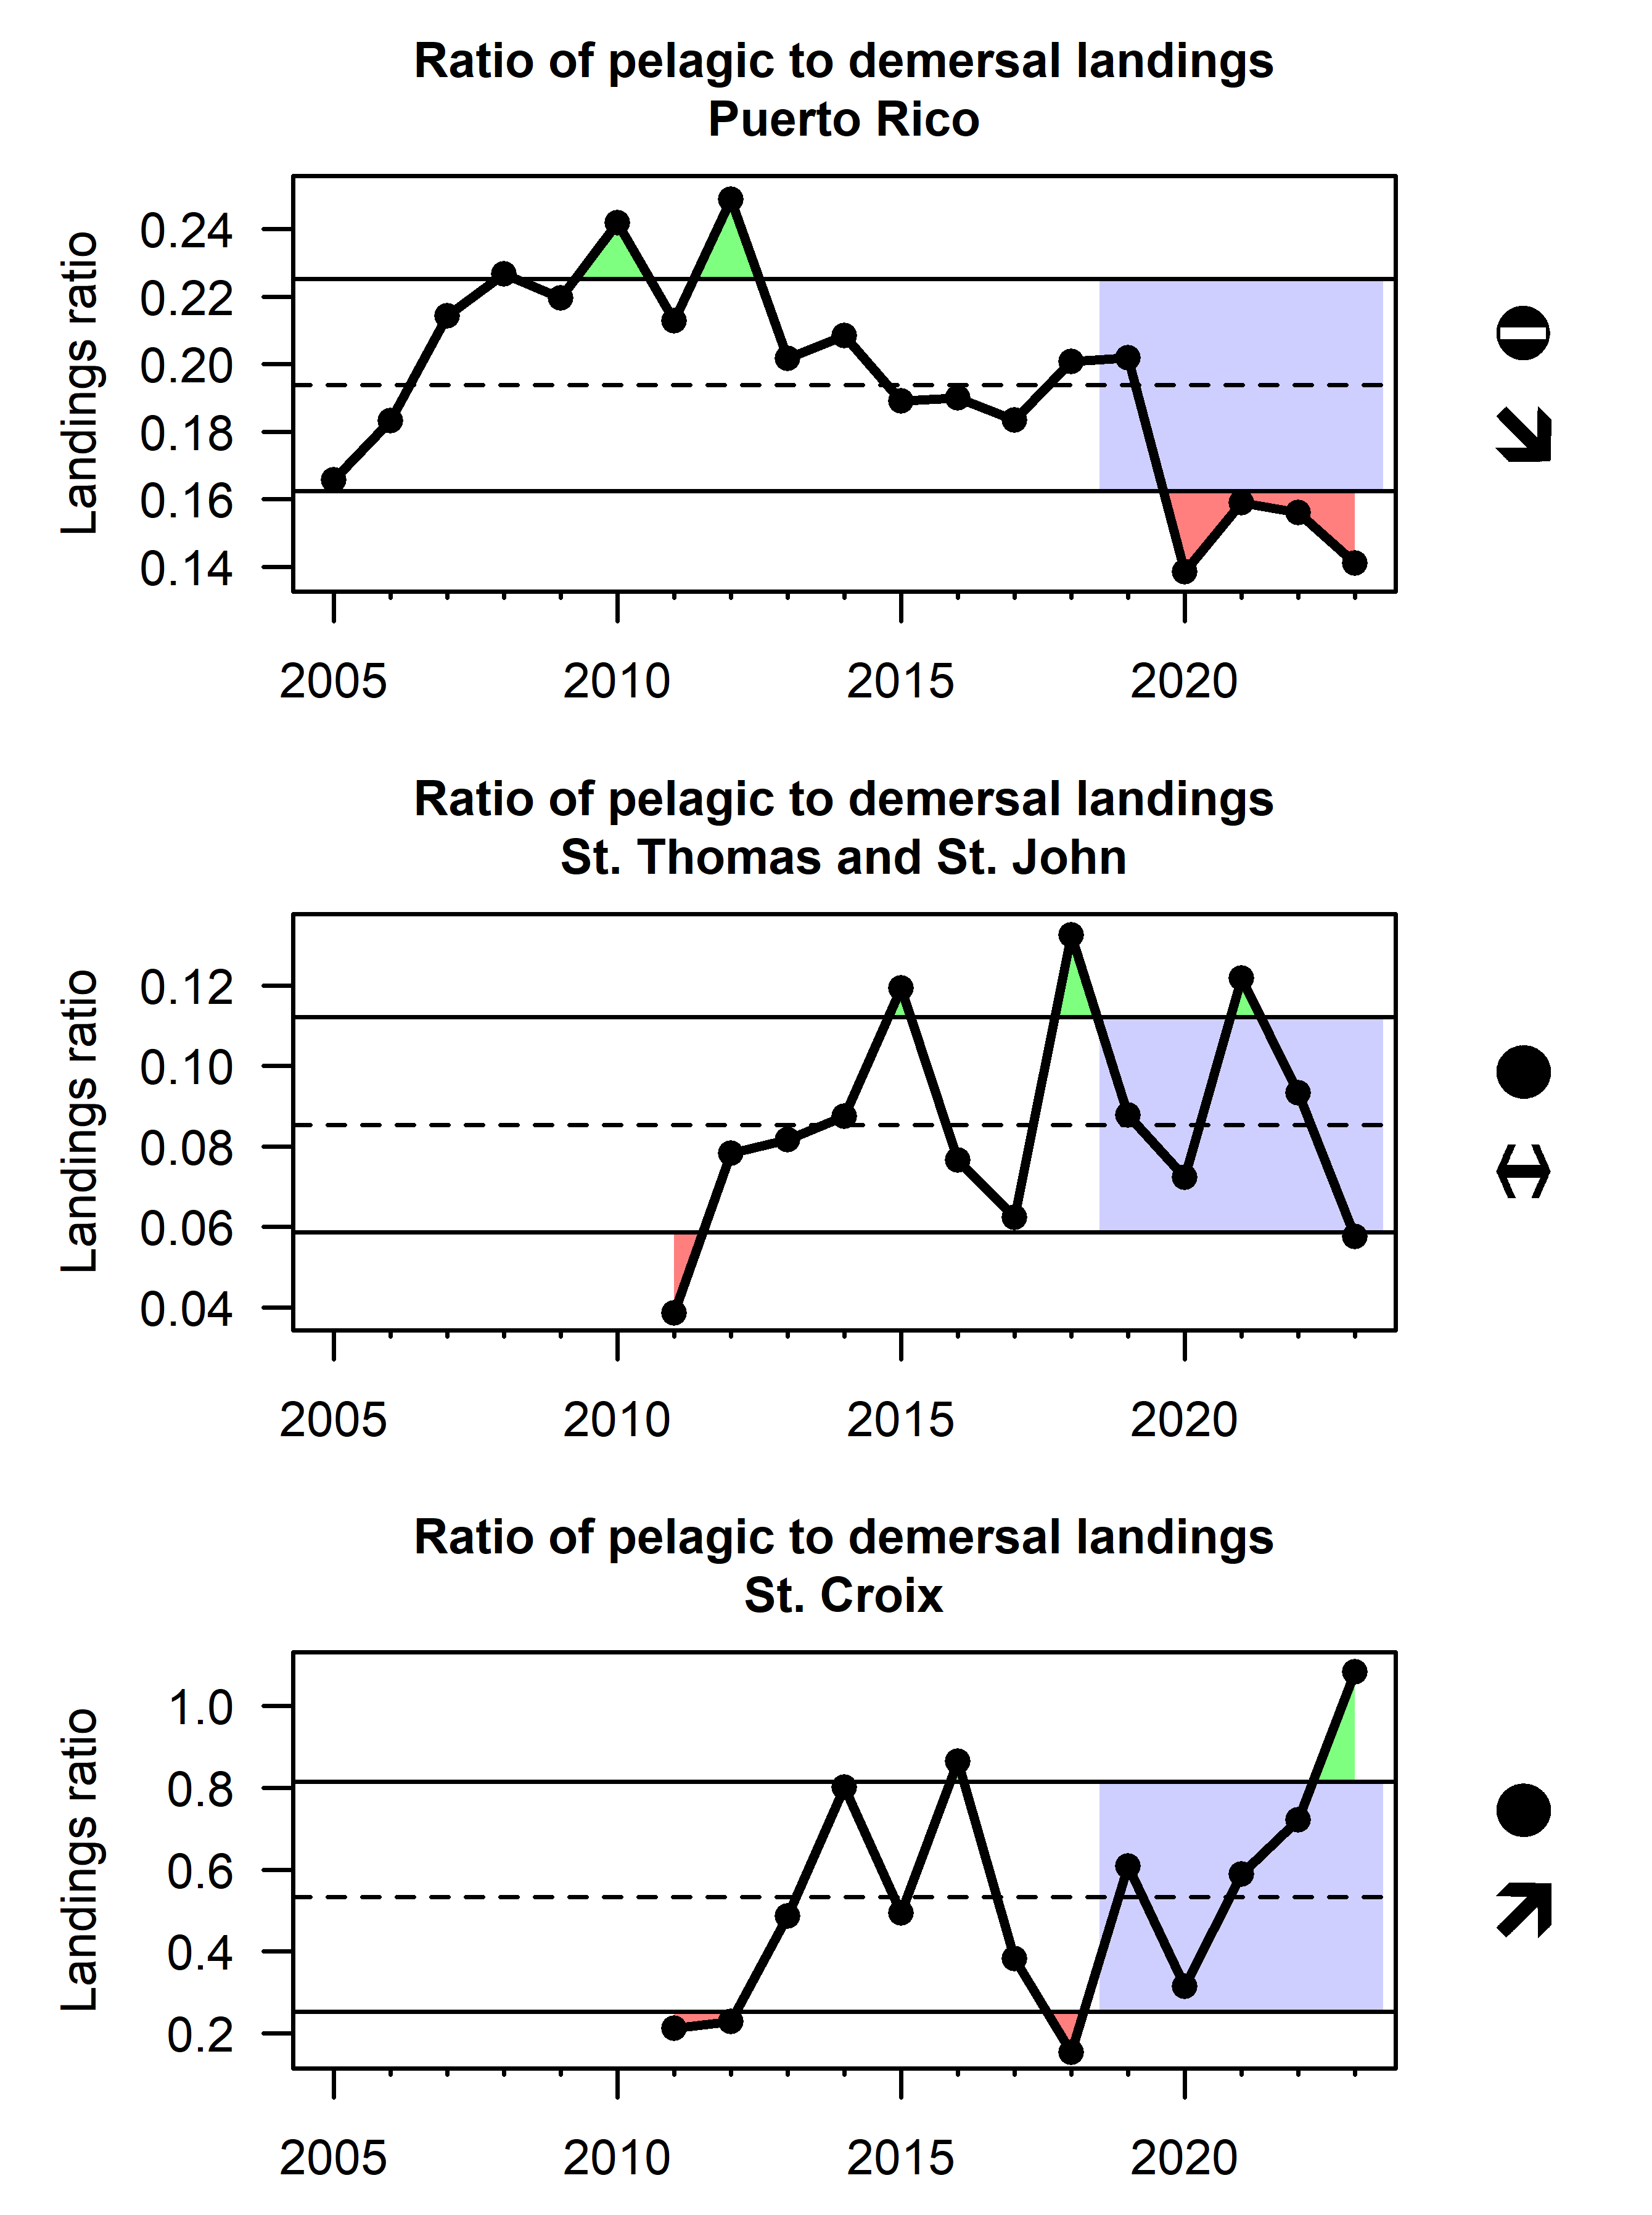
\includegraphics{indicator_plots/PD_ratio_plot_final.png}

}

\caption{\label{fig-PD}PD ratio}

\end{figure}%

\subsection{Maximum length and size
structure}\label{maximum-length-and-size-structure}

The average maximum length of a species in the landings has been
proposed as an indicator of whether large-bodies species have been
depleted and are no longer fished (Rochet and Trenkel 2003). The Lmax
indicator is derived by assigning a maximum body length for each species
(as reported in FishBase) and then calculating the average body length
for the landings in each year, or the proportion of landings within
different Lmax classes (based on the Caribbean Commercial Landings
database). The average maximum length in the landings has been
relatively stable across all islands in the U.S. Caribbean with an
uptick across all islands in the last five years; this is partially due
to a shift to more pelagic species in the landings
(Figure~\ref{fig-avgLmax}).

\begin{figure}

\centering{

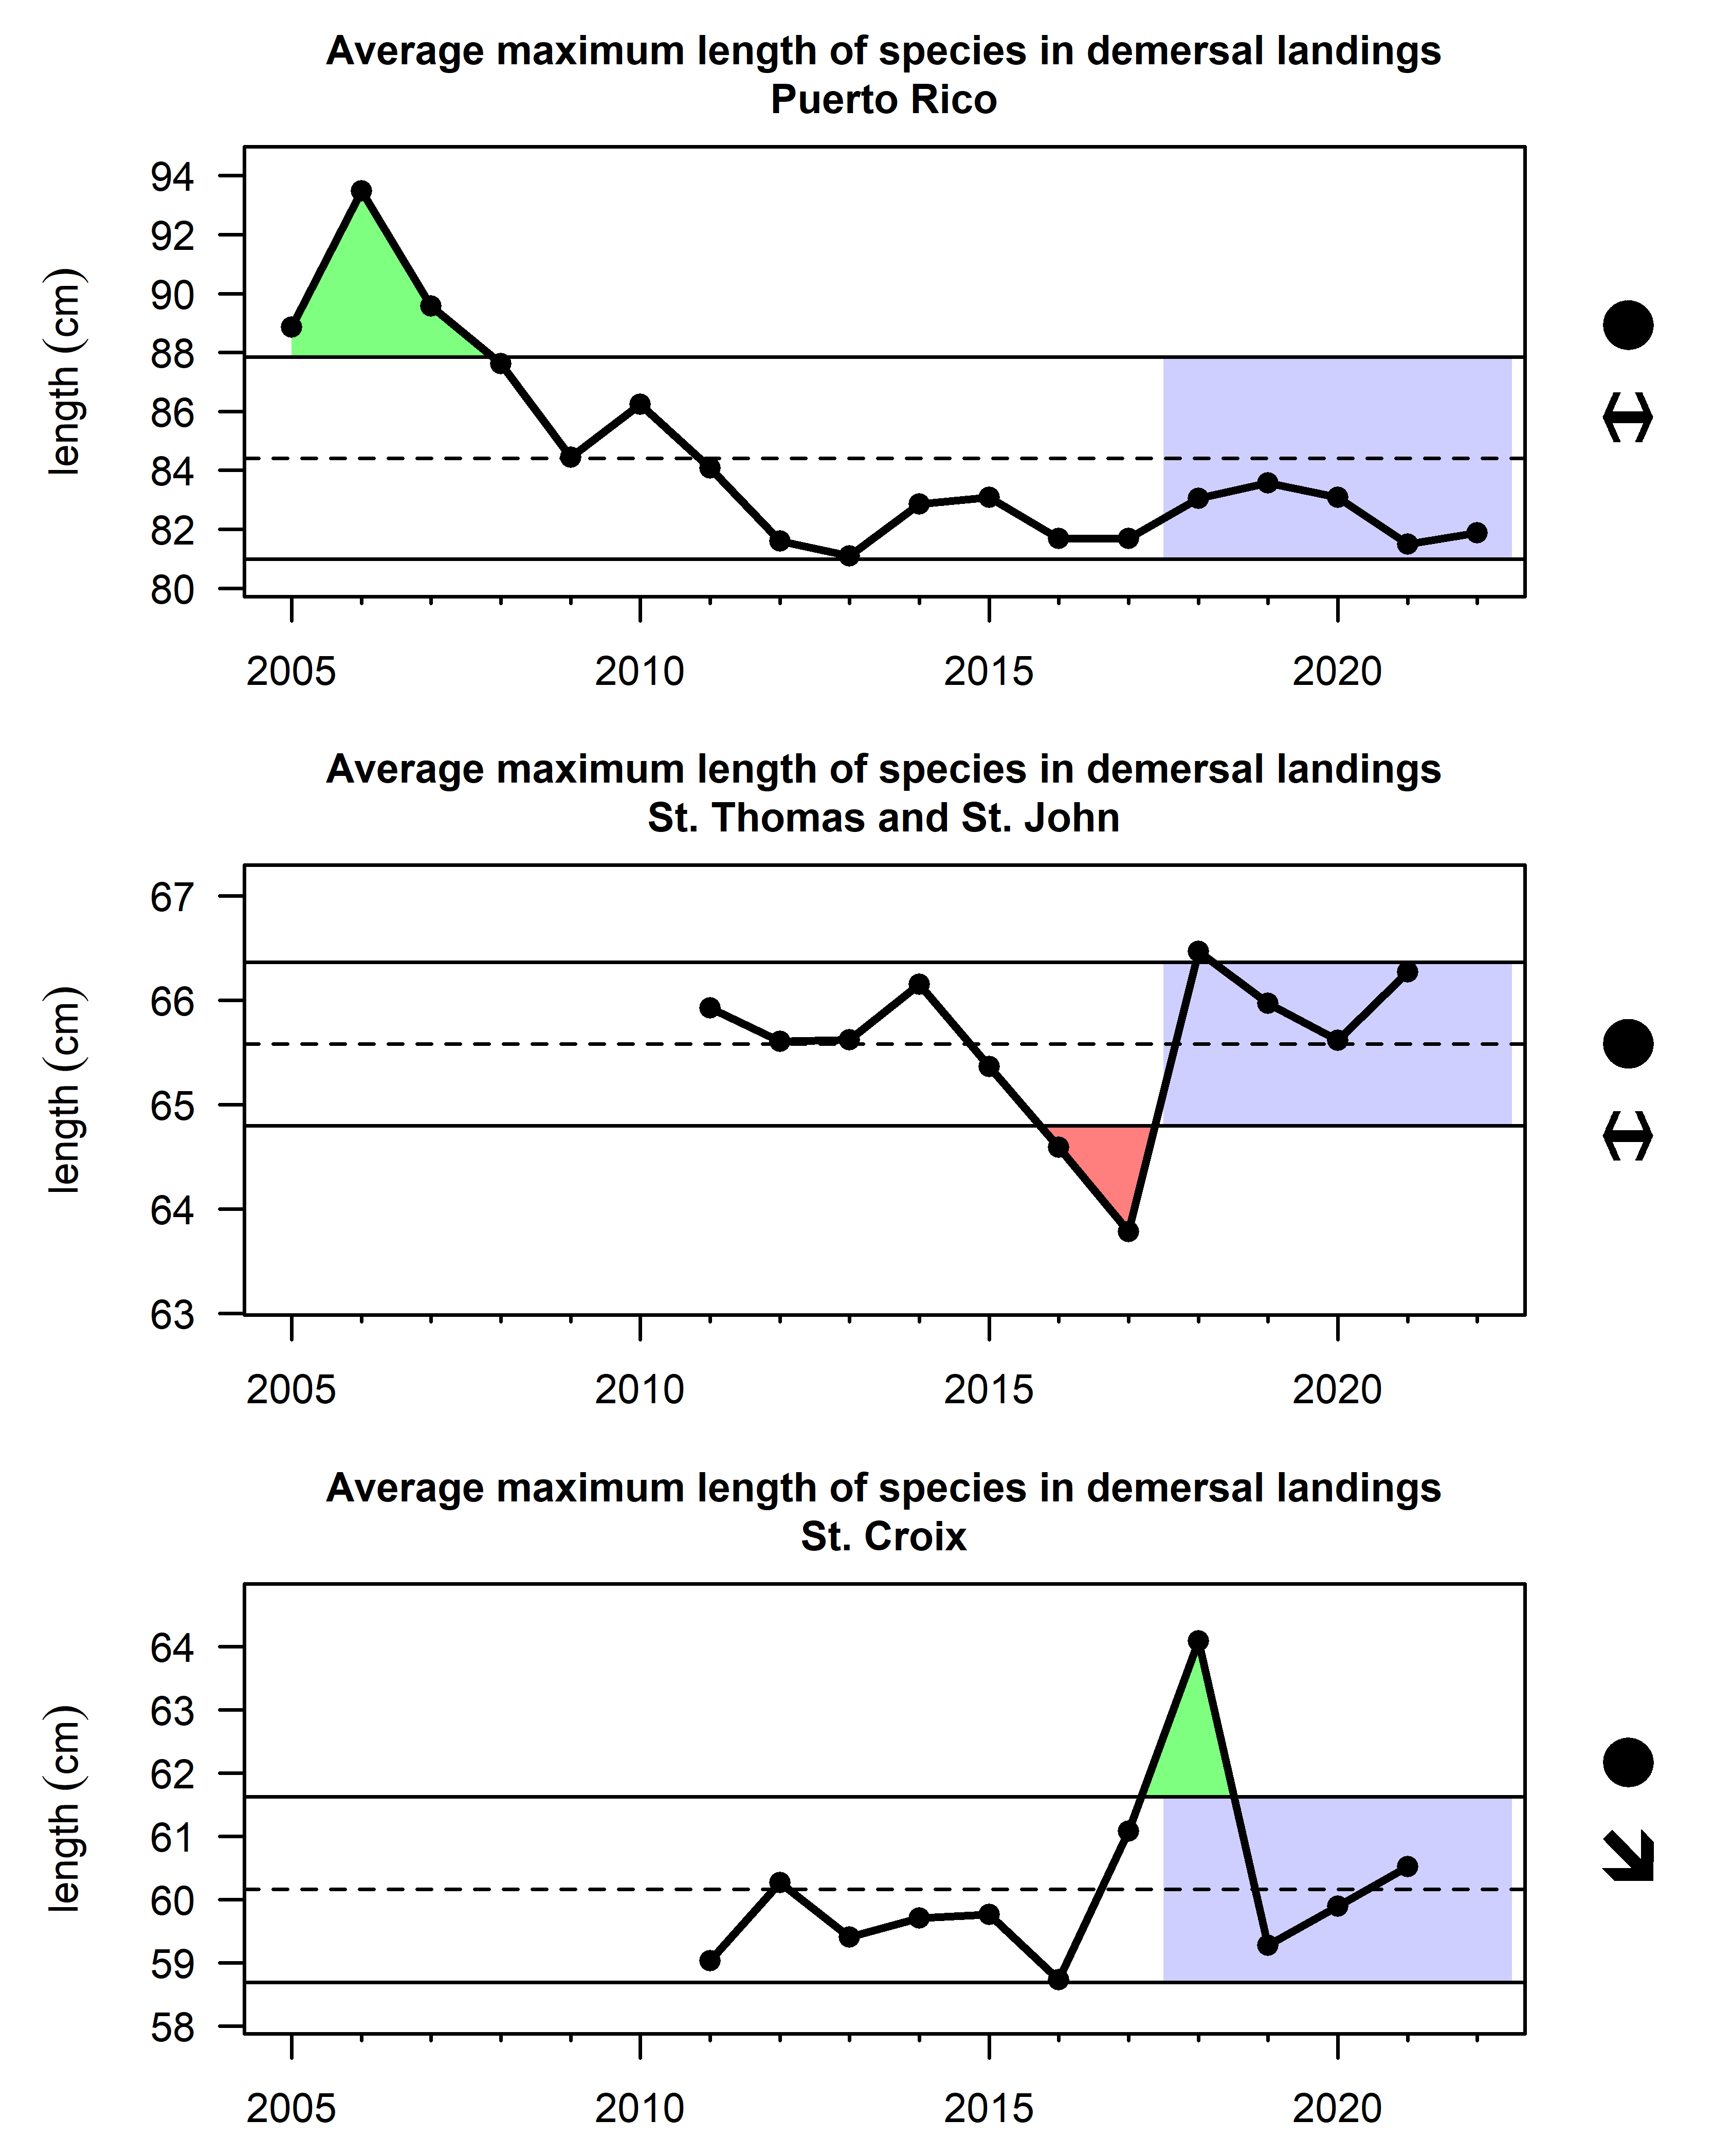
\includegraphics{indicator_plots/avgLmax_plot_final.png}

}

\caption{\label{fig-avgLmax}Average Lmax}

\end{figure}%

In Puerto Rico, there is an overall increasing trend of ``plate-sized''
fish in the 60-100cm category which is driven by increased landings of
deepwater snapper species, yellowtail snapper, hogfish and red hind,
while a decrease in the 100-200cm Lmax group is driven by declining
catches of mackerels, large rare parrotfishes, tunas, and some large
groupers (Figure~\ref{fig-PRLmax}).

\begin{figure}

\centering{

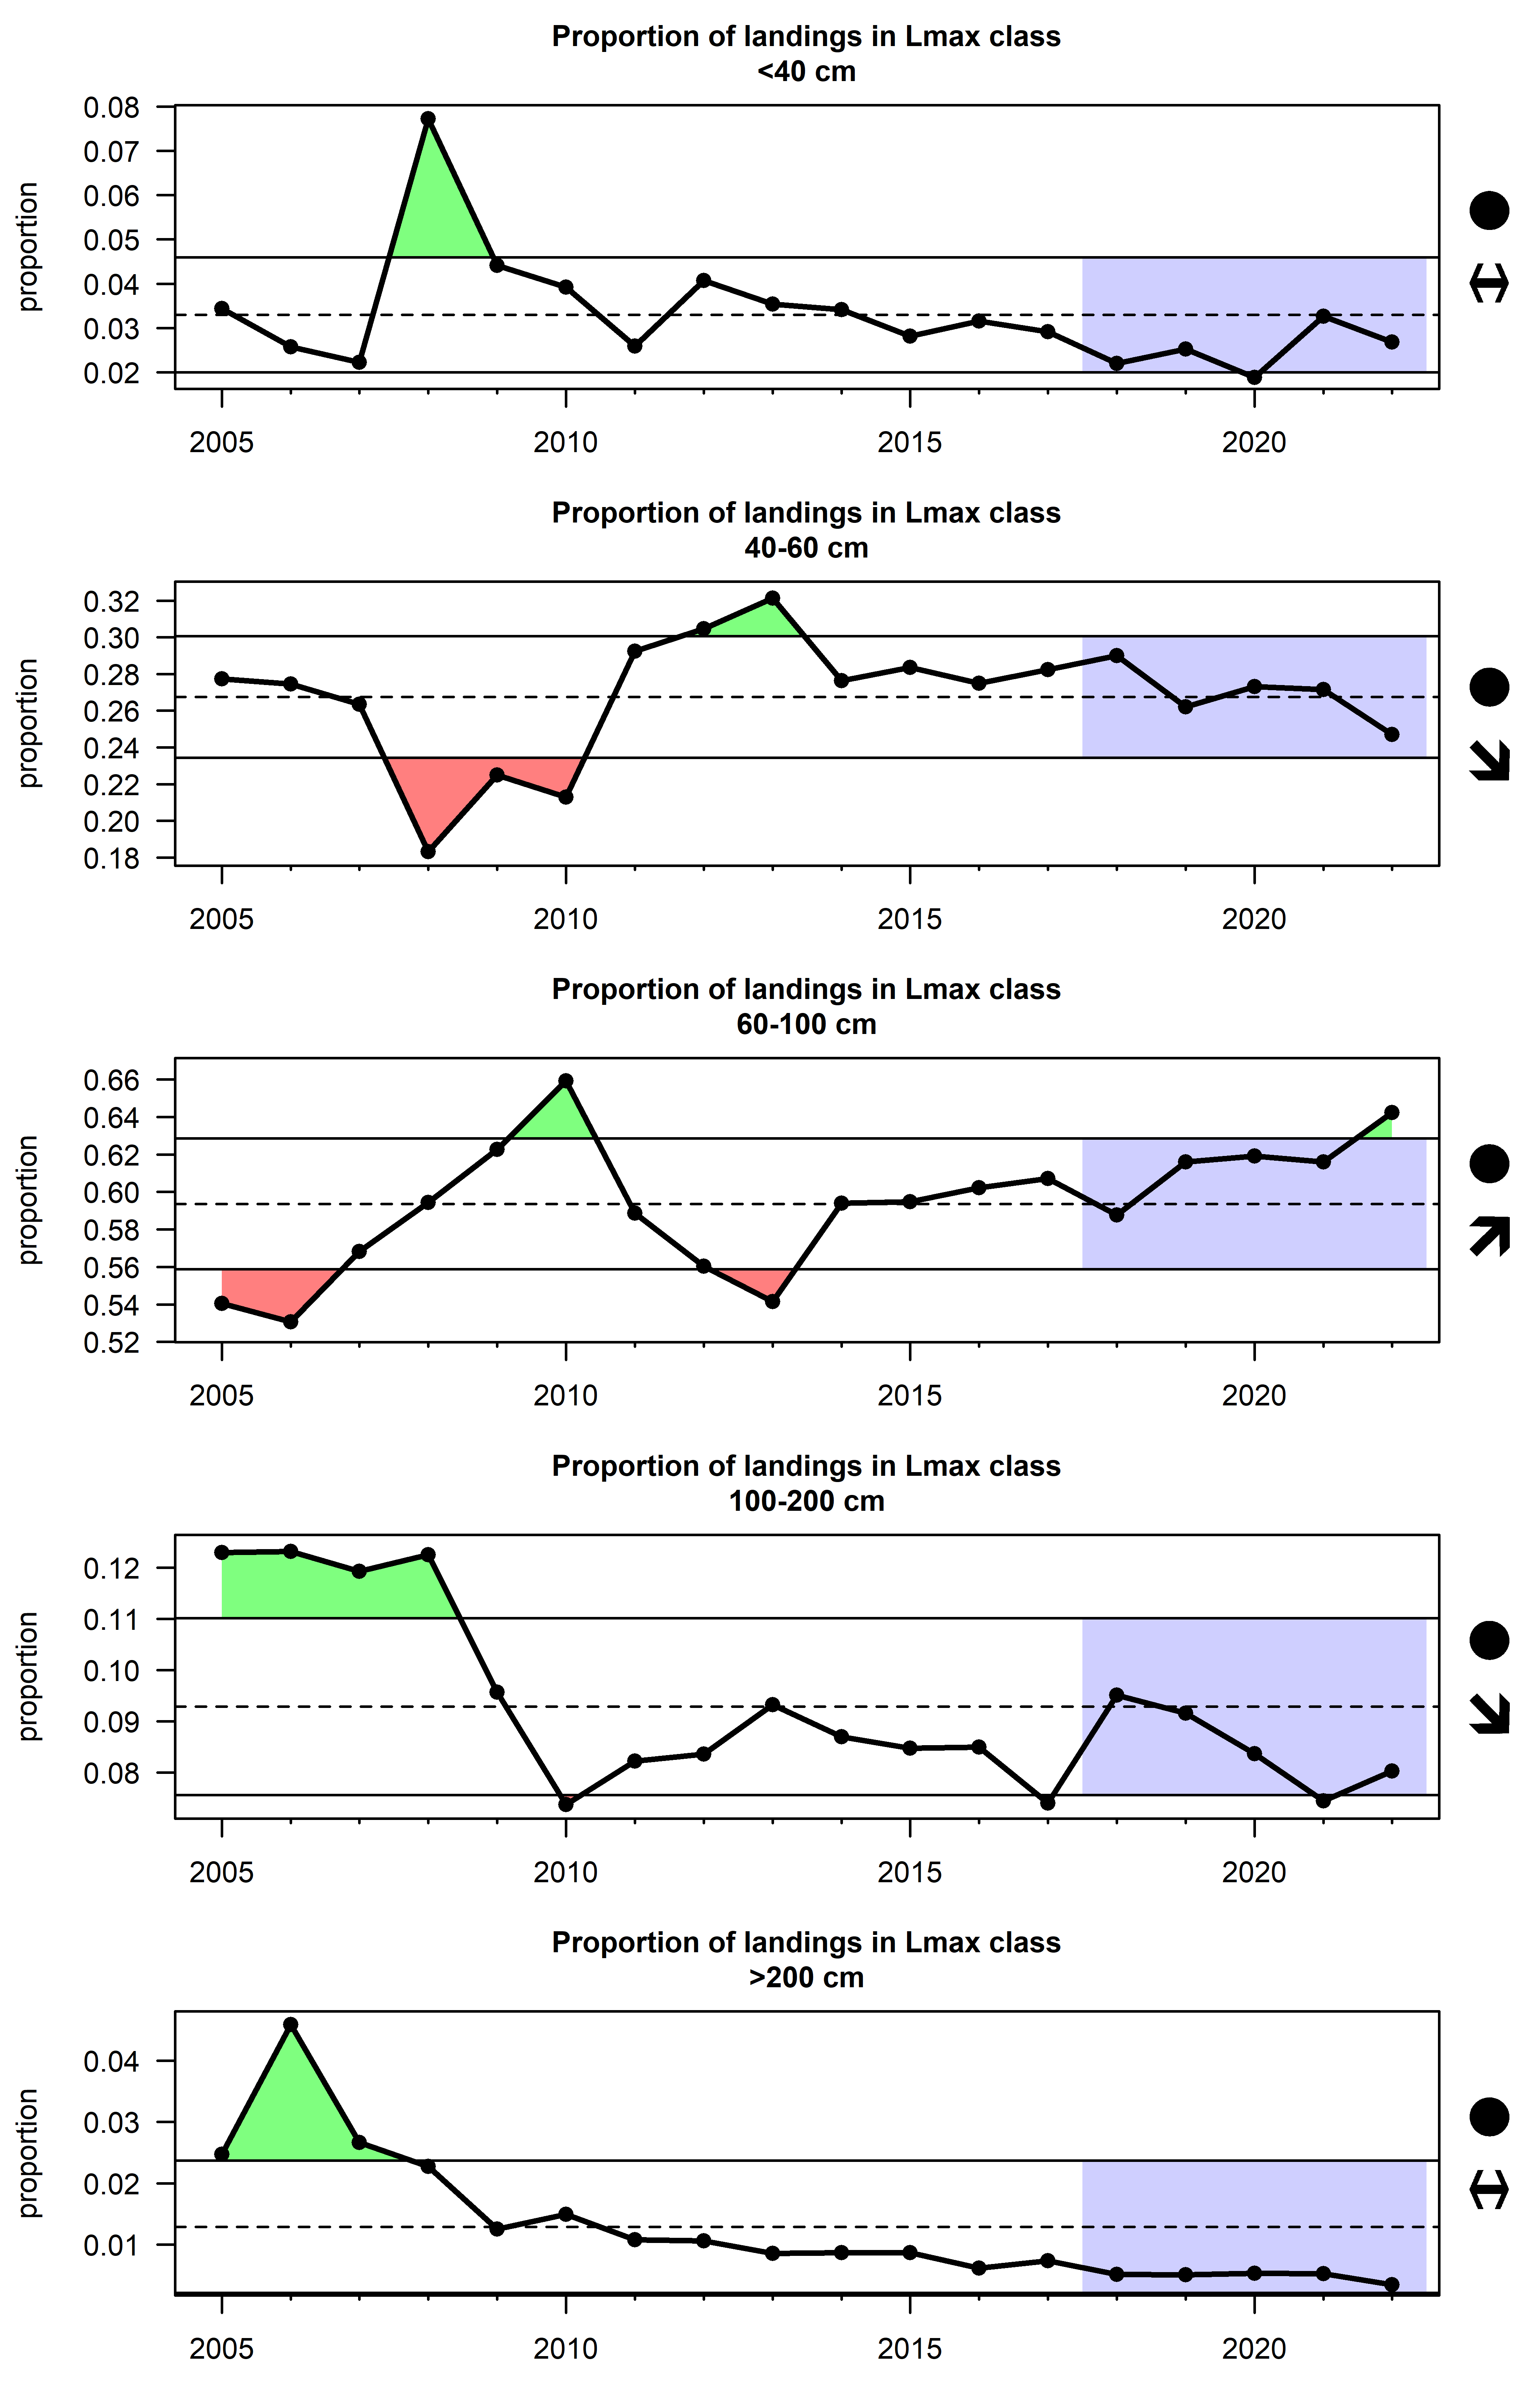
\includegraphics{indicator_plots/PR_Lmax_classes_plot_final.png}

}

\caption{\label{fig-PRLmax}PR Lmax}

\end{figure}%

In St.~Thomas there is a notable decrease in the smallest size class
(dominated by surgeonfishes and longspine squirrelfish landings) while
there are increases in the larger size classes due to increasing catches
of tunas and mackerels, as well as red grouper
(Figure~\ref{fig-STTLmax}).

\begin{figure}

\centering{

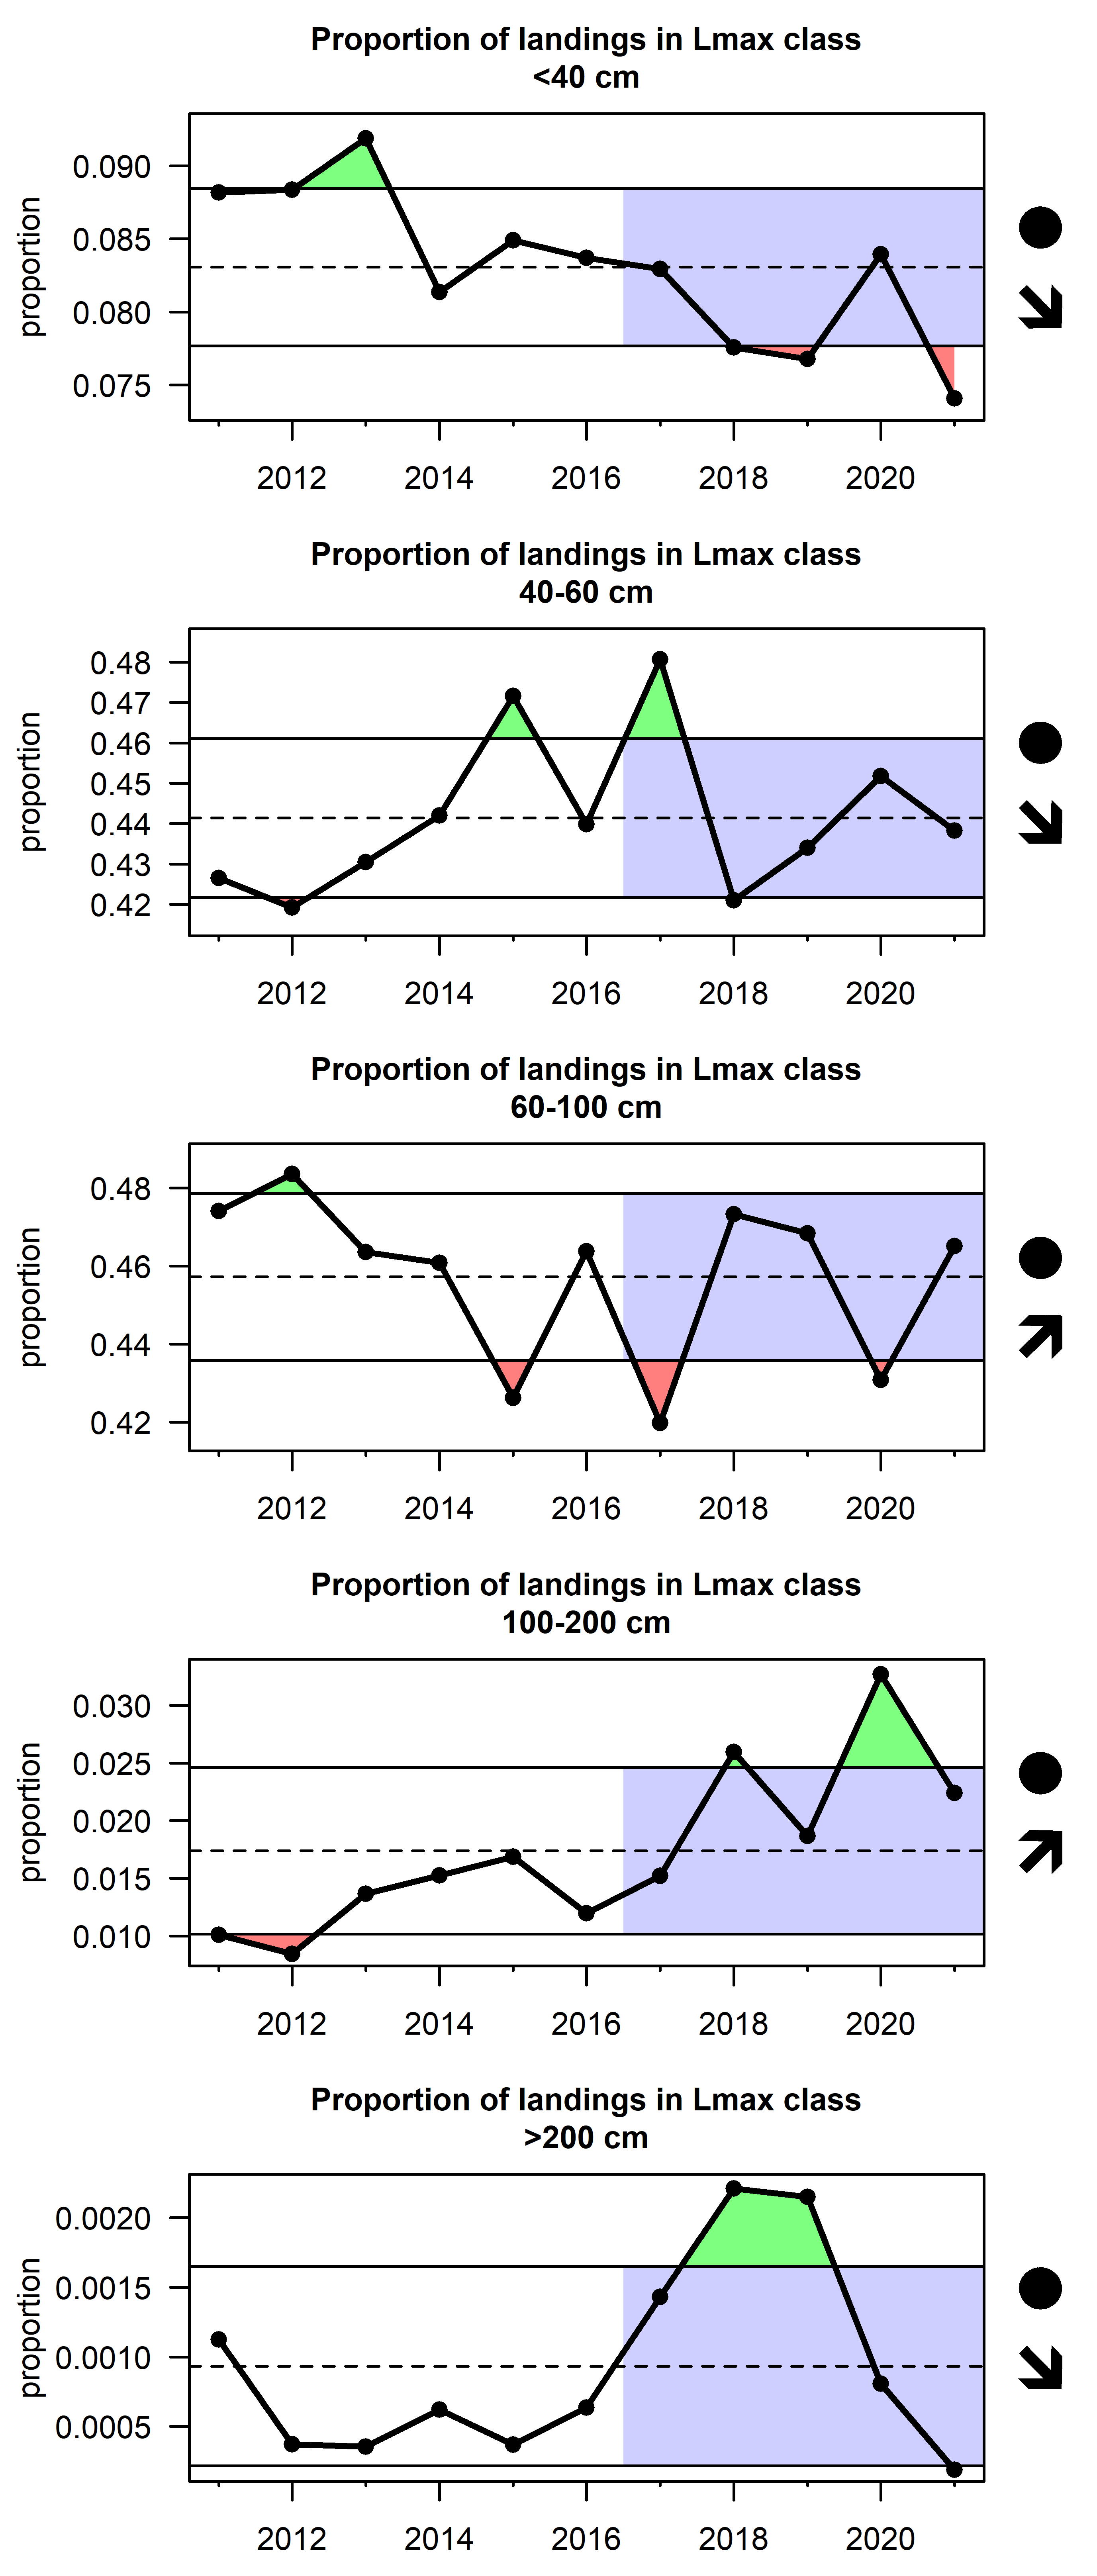
\includegraphics{indicator_plots/STT_Lmax_classes_plot_final.png}

}

\caption{\label{fig-STTLmax}STT Lmax}

\end{figure}%

In St.~Croix\ldots{} Lmax\_cat == ``(0,40'') driven by redband
parrotfish and princess parrotfish. also herrings and surgeonfishes
Lmax\_cat == ``(60,100'') mainly stoplight and queen parrotfishes. Also
blackfin and silk snapper and red hind Lmax\_cat == ``(100,200'') tunas
(little tunny) and king mackerel (Figure~\ref{fig-STXLmax}).

\begin{figure}

\centering{

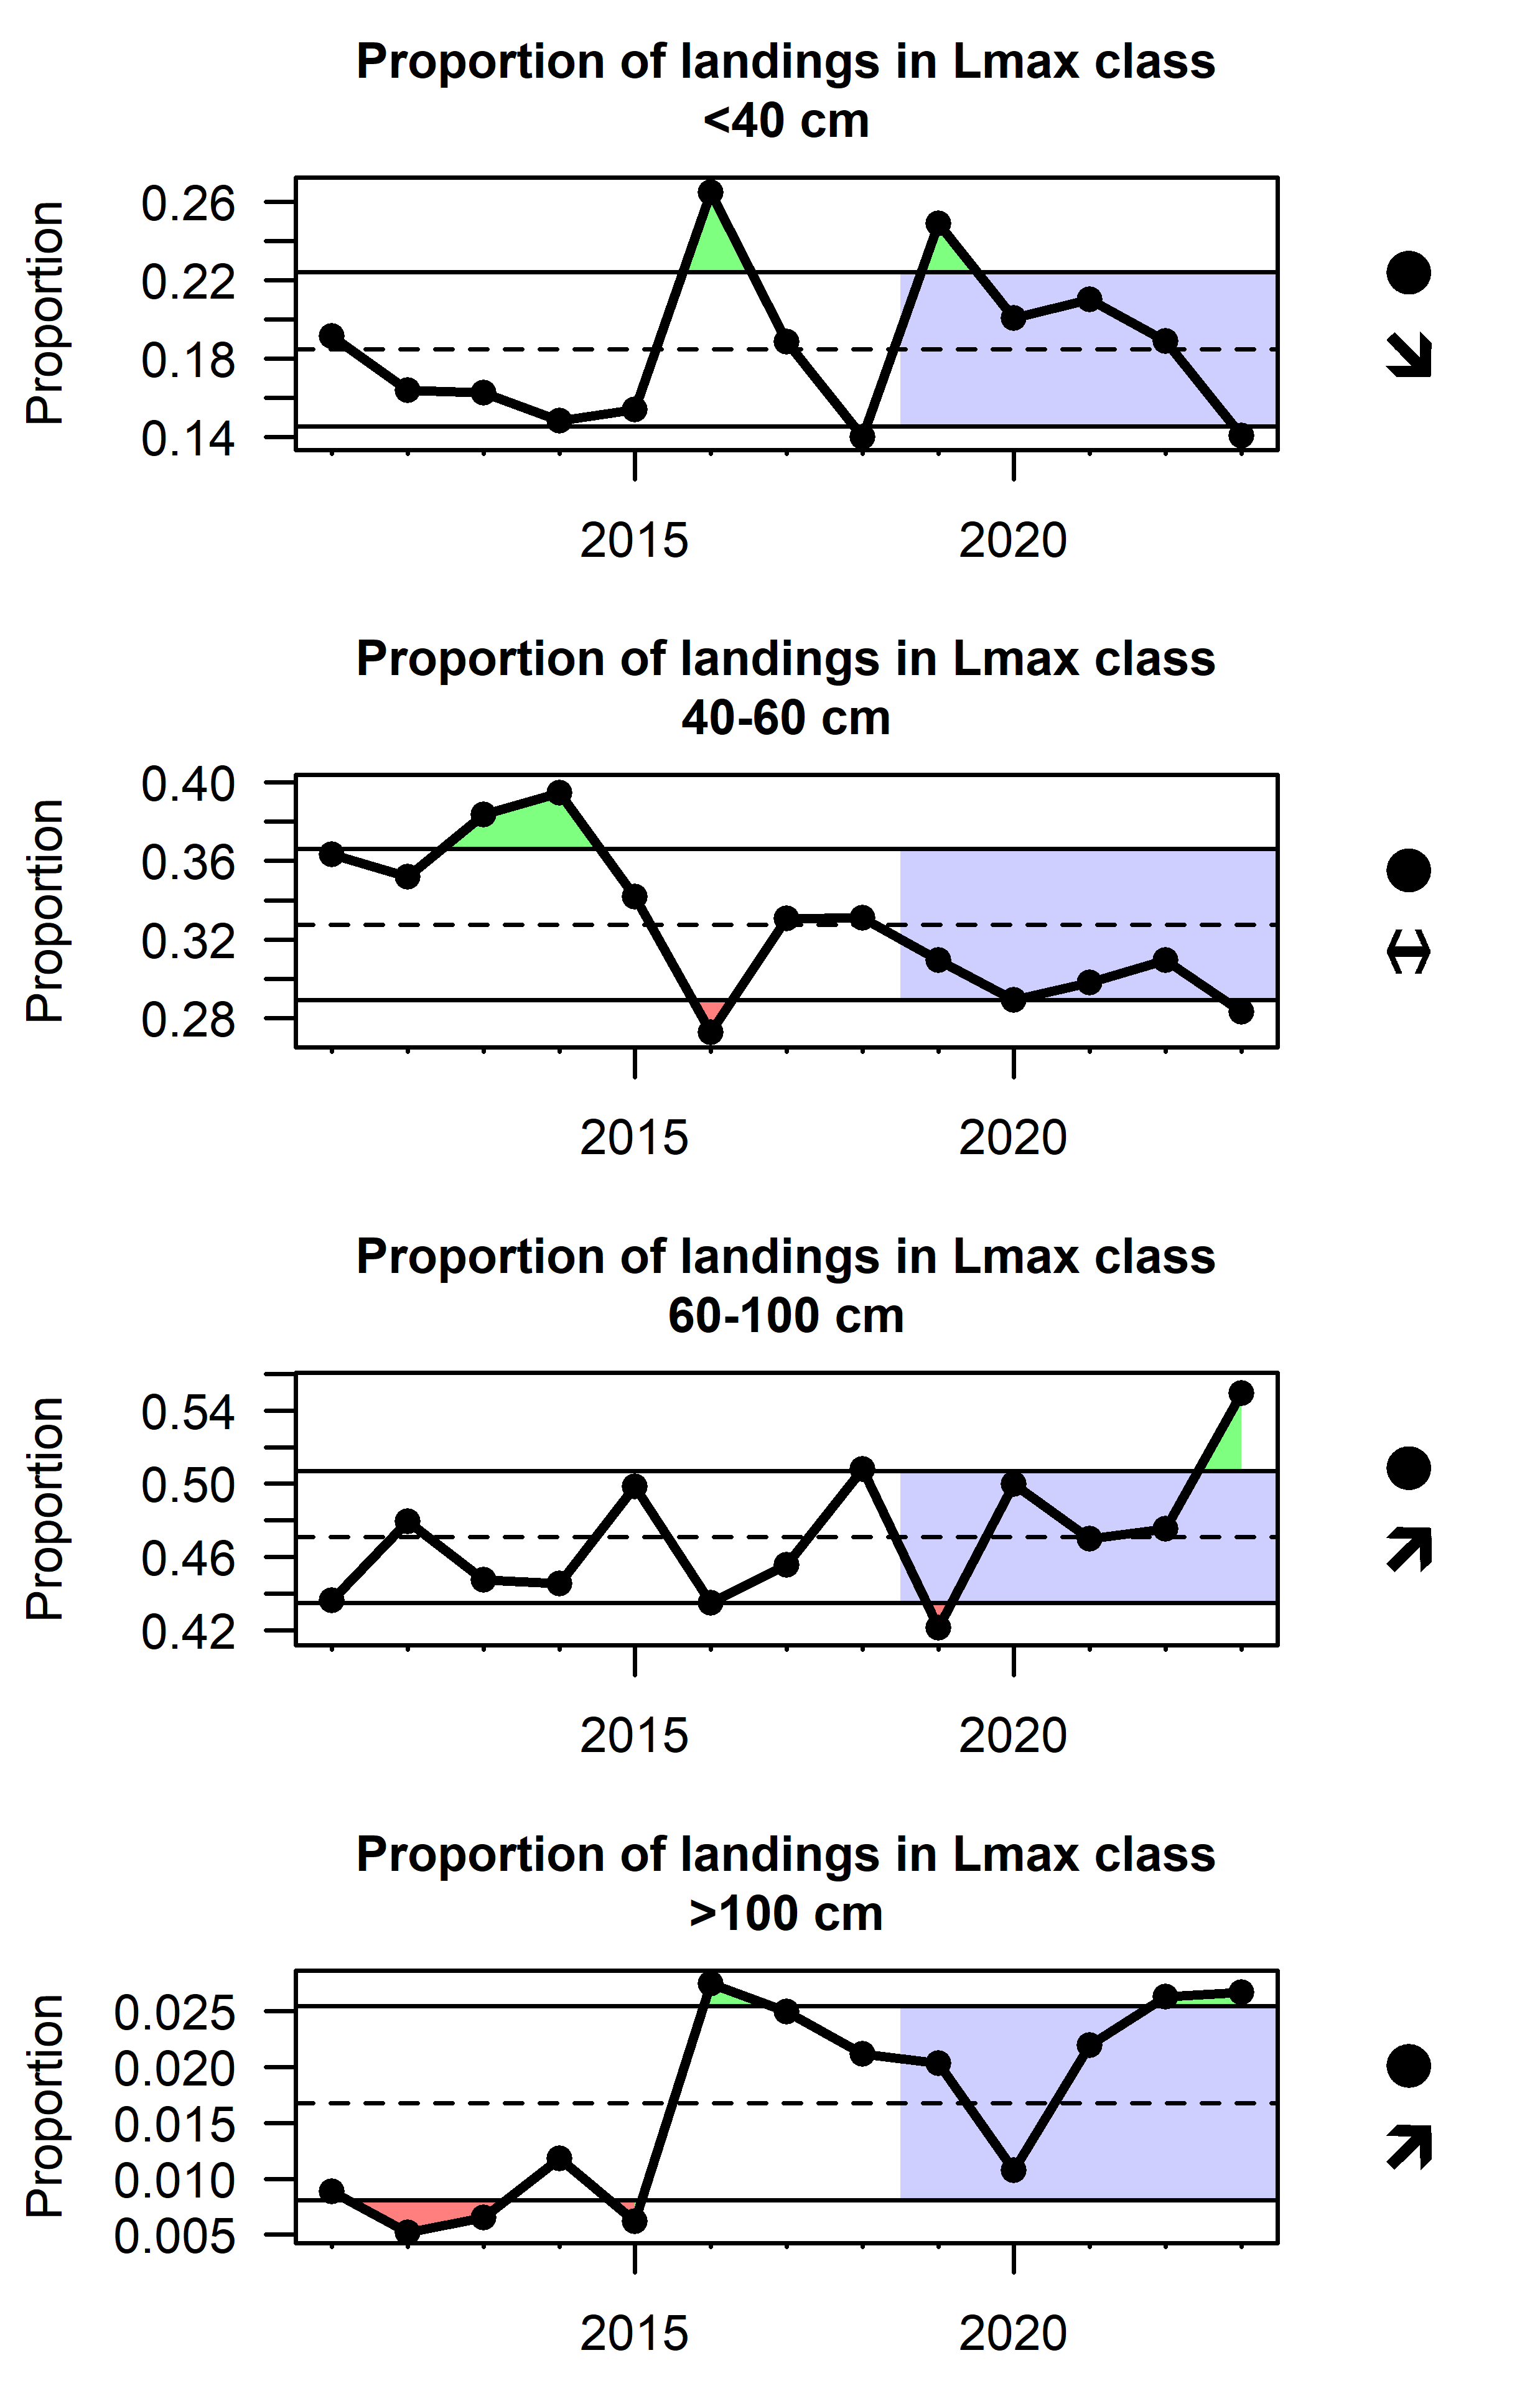
\includegraphics{indicator_plots/STX_Lmax_classes_plot_final.png}

}

\caption{\label{fig-STXLmax}STX Lmax}

\end{figure}%

\subsection{Commercial landings}\label{commercial-landings}

Total landings of conch, lobster, and finfish indicate the ability of
U.S. Caribbean fisheries to provide food and revenues, and may be driven
by a combination of trends in underlying abundance, market demand, and
fishing effort. Self-reported landings from the Caribbean Commercial
Landings Data were compiled; data were originally compiled by paper
logbooks, but starting in 2020 some trips in Puerto Rico were reported
using electronic reporting (a telephone application). Since 2005,
lobster landings have increased in Puerto Rico and decreased in the
USVI, with particularly low values in 2017-18 for St.~Thomas and 2018-19
for St.~Croix. Conch landings have been more variable with little trend
over time, though there was a sudden decrease in Puerto Rico conch
landings in 2020. Landings of other species have decreased significantly
over time, particularly starting in 2010 (Figure~\ref{fig-totalland}).
This coincides with initial implementation of annual catch limits in
U.S. Caribbean federal waters and may be caused by changes in reporting
rather than true reductions in catch.

\begin{figure}

\centering{

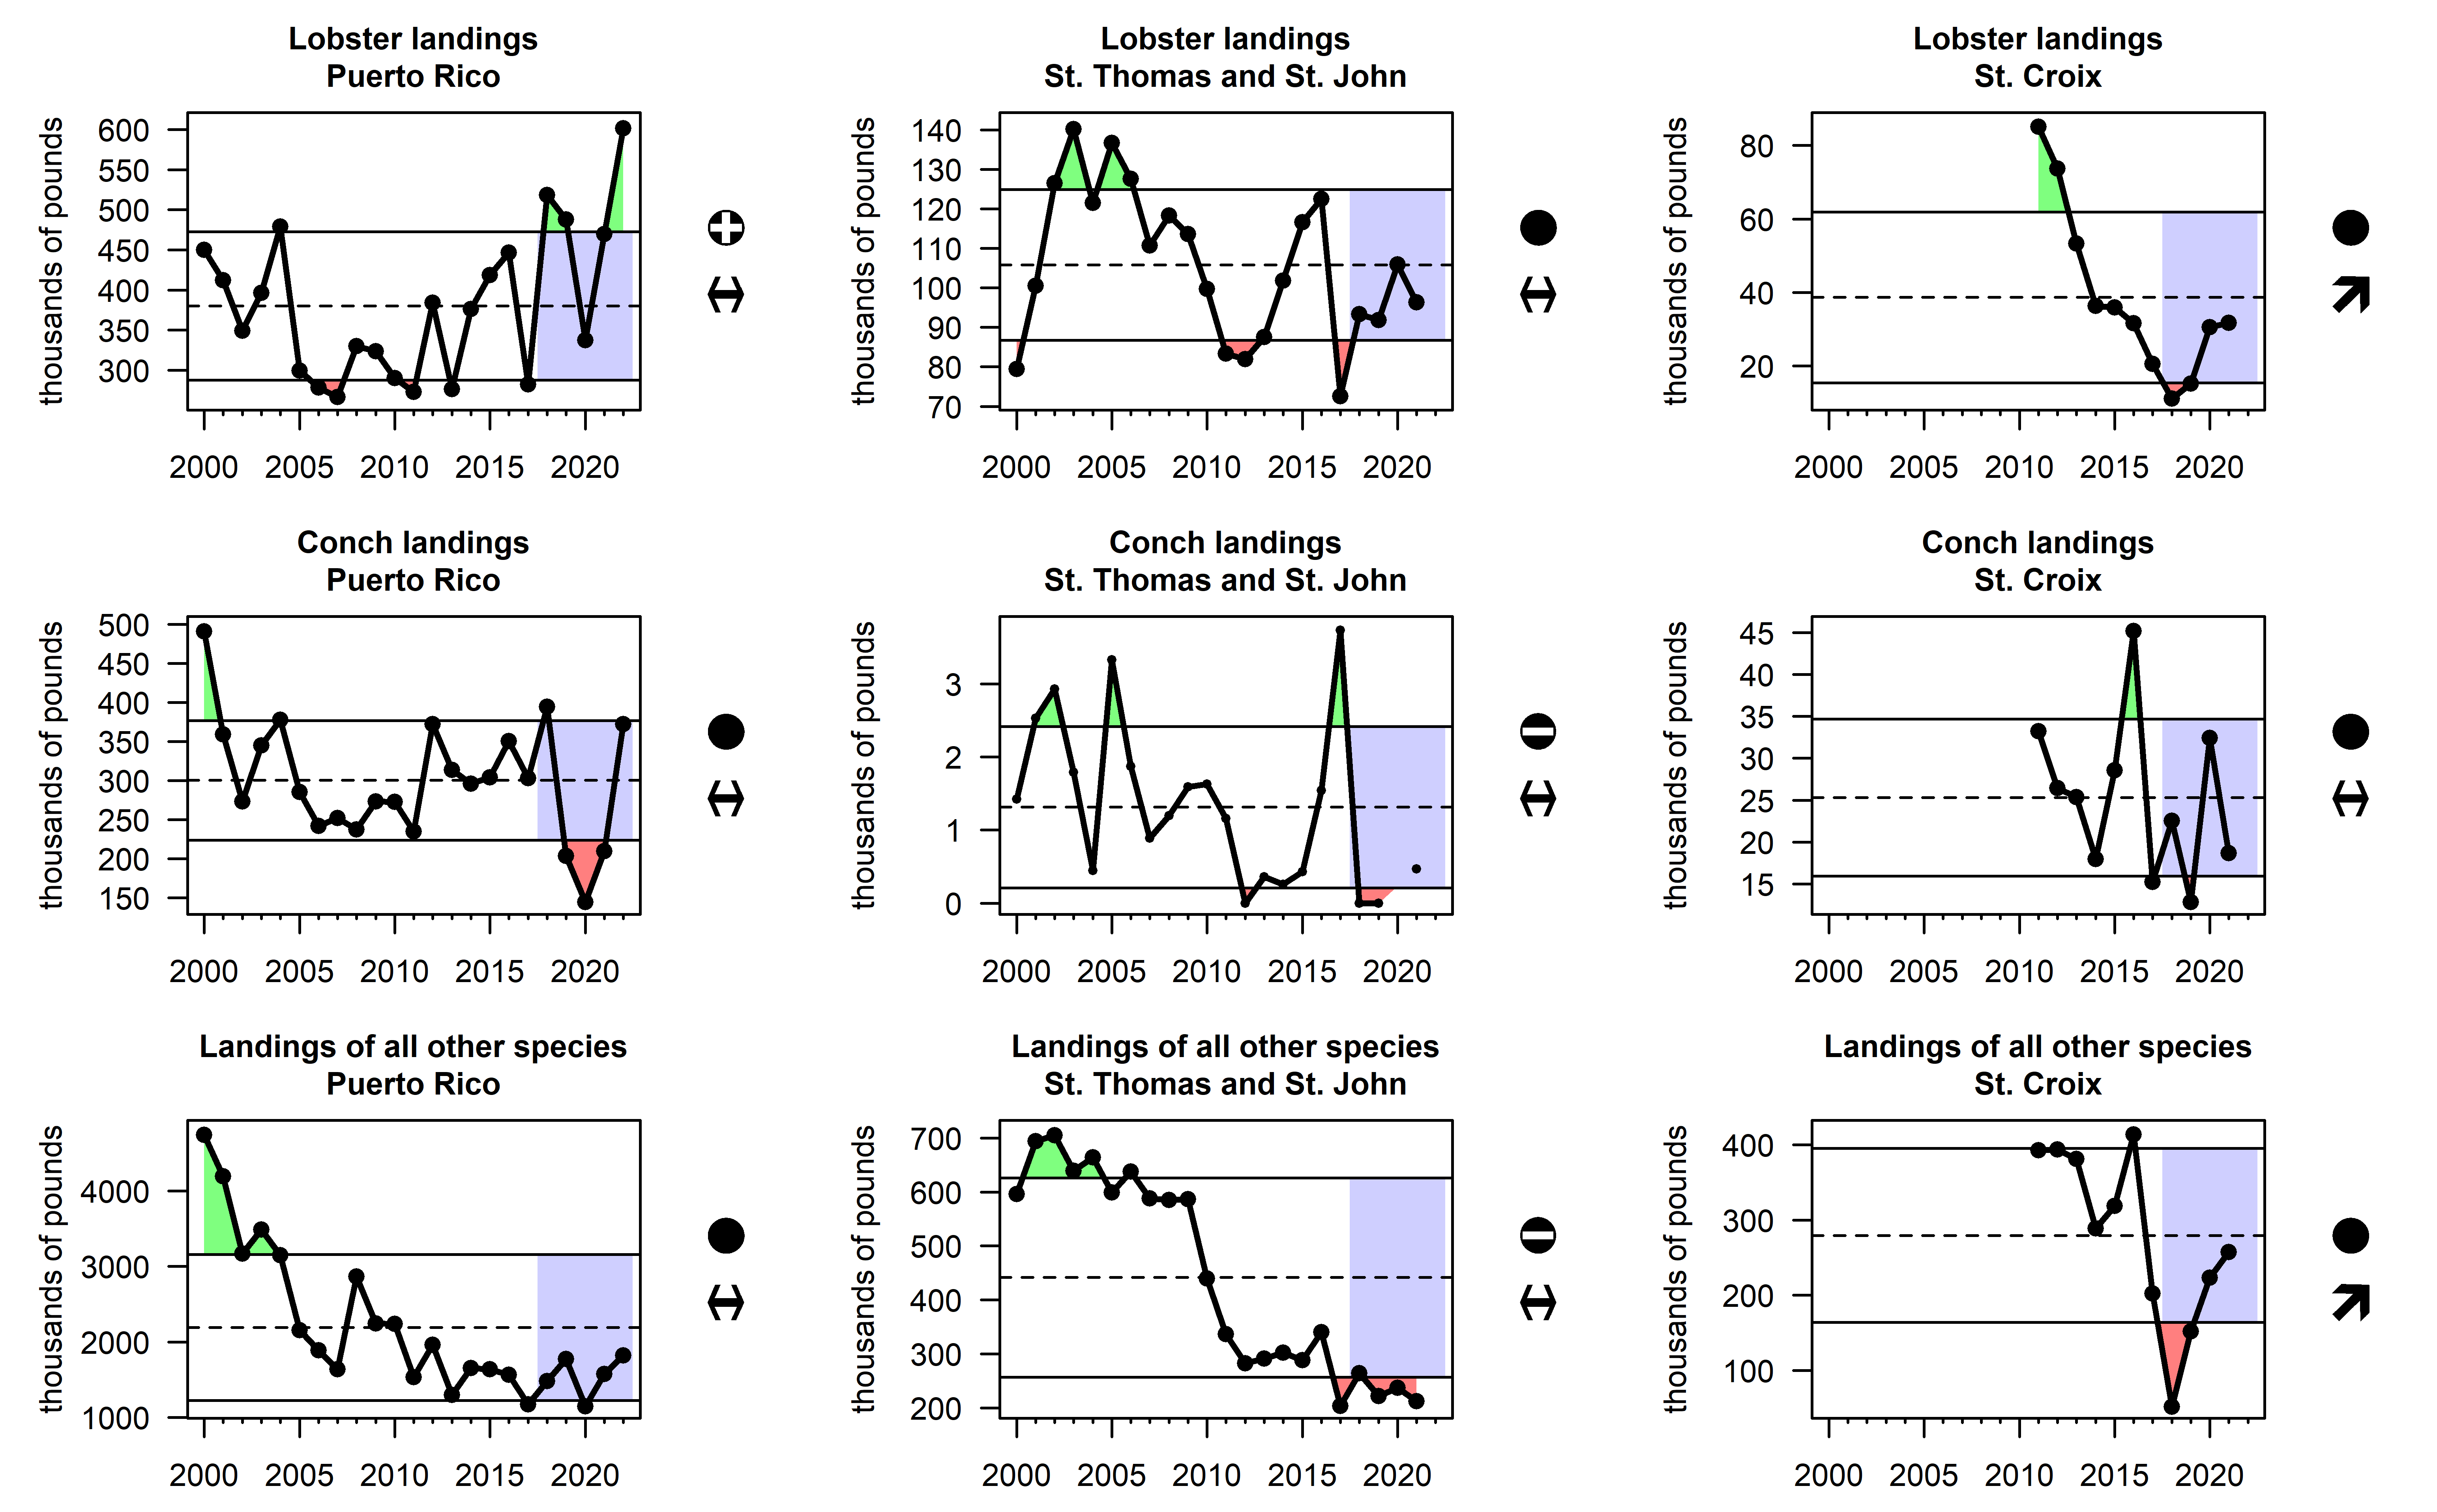
\includegraphics{indicator_plots/total_landings_plot_final.png}

}

\caption{\label{fig-totalland}Total landings}

\end{figure}%

\section{Socioeconomic health}\label{socioeconomic-health}

\subsection{Total, lobster and conch
revenues}\label{total-lobster-and-conch-revenues}

The relative revenue contribution to commercial fisheries by species
conveys the changing reliance on different species across the U.S.
Caribbean. Revenues were calculated from the Caribbean Commercial
Landings data based on the weight of landings in each trip and the
reported price; anomalously high prices and missing values were replaced
by the overall average price for the given species group. In Puerto
Rico, approximately a third of the revenues have consistently come from
snapper species; snappers are followed by lobster and conch, which were
both increasing in their revenue contribution up to 2017
(Figure~\ref{fig-perlandPR}). In St.~Thomas and St.~John, there has also
been increasing dependence on lobster which supplies roughly a third of
the revenues for those islands (Figure~\ref{fig-perlandSTT}). Revenues
in St.~Croix are less dominated by a single species group, but
parrotfishes, tunas and mackerels, lobsters, snappers, and dolphinfish
make up approximately 75\% of the revenues
(Figure~\ref{fig-perlandSTX}).

\begin{figure}

\centering{

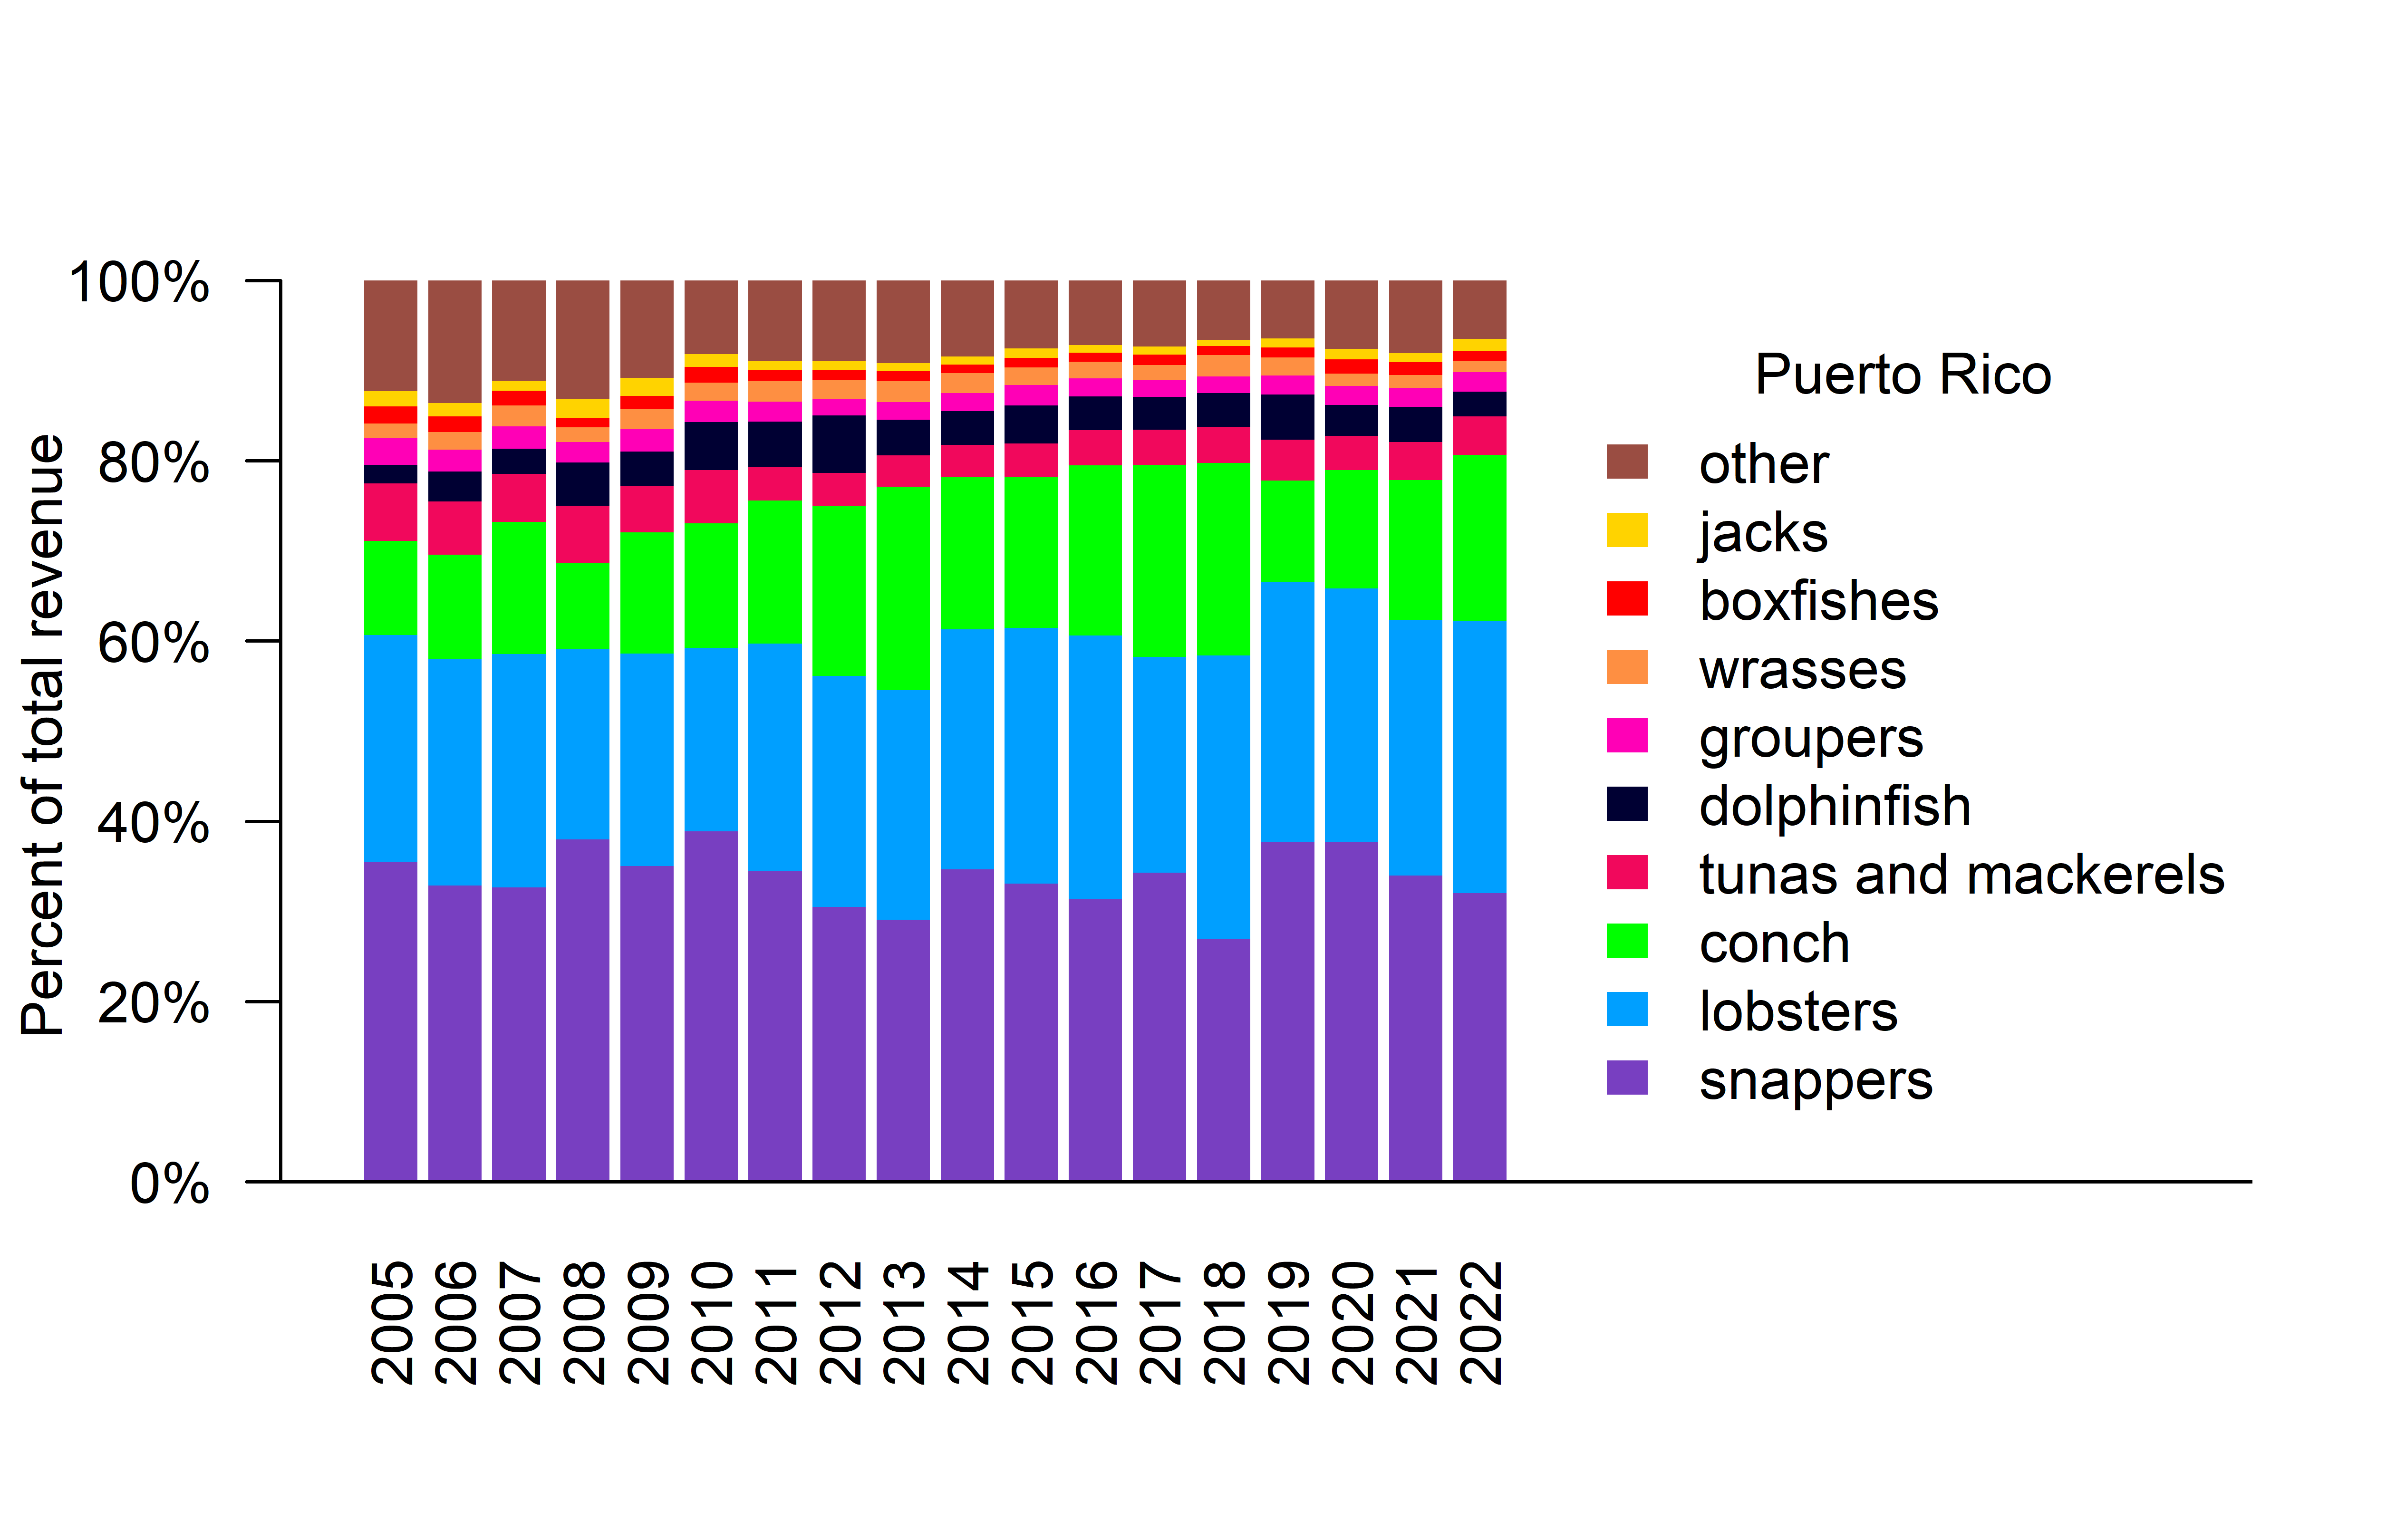
\includegraphics{indicator_plots/per_landings_PR.png}

}

\caption{\label{fig-perlandPR}PR}

\end{figure}%

\begin{figure}

\centering{

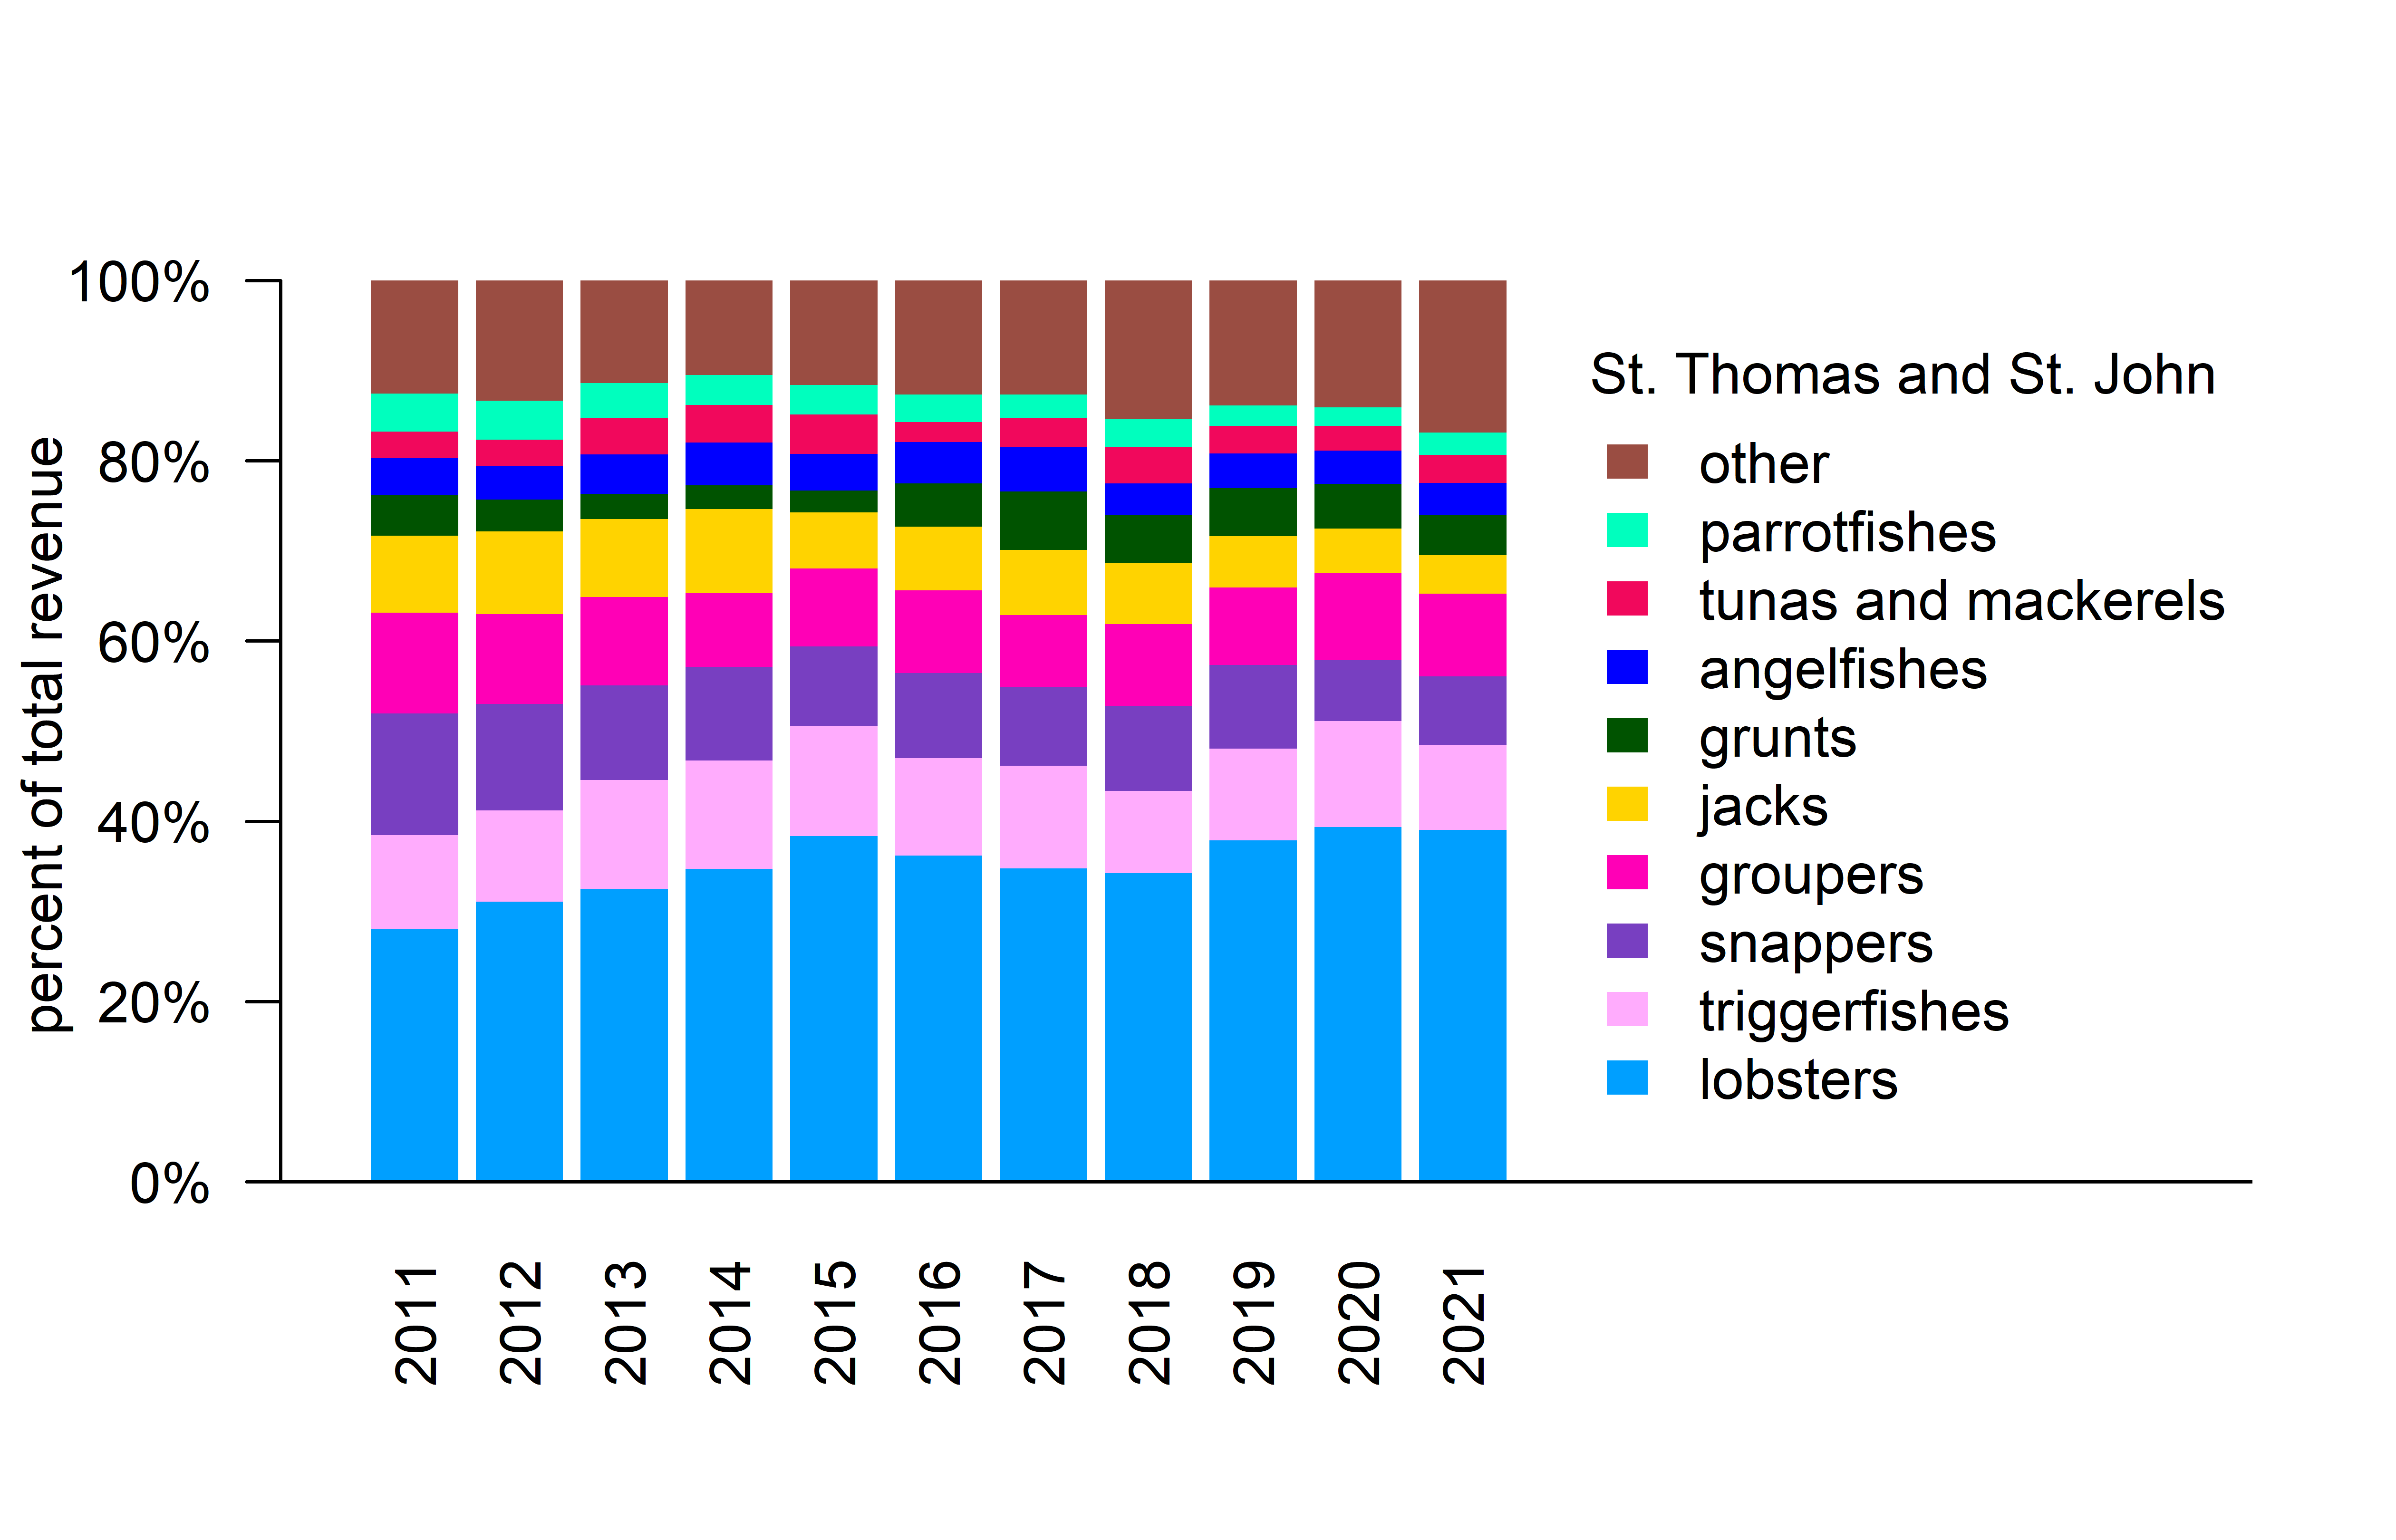
\includegraphics{indicator_plots/per_landings_STT.png}

}

\caption{\label{fig-perlandSTT}STT}

\end{figure}%

\begin{figure}

\centering{

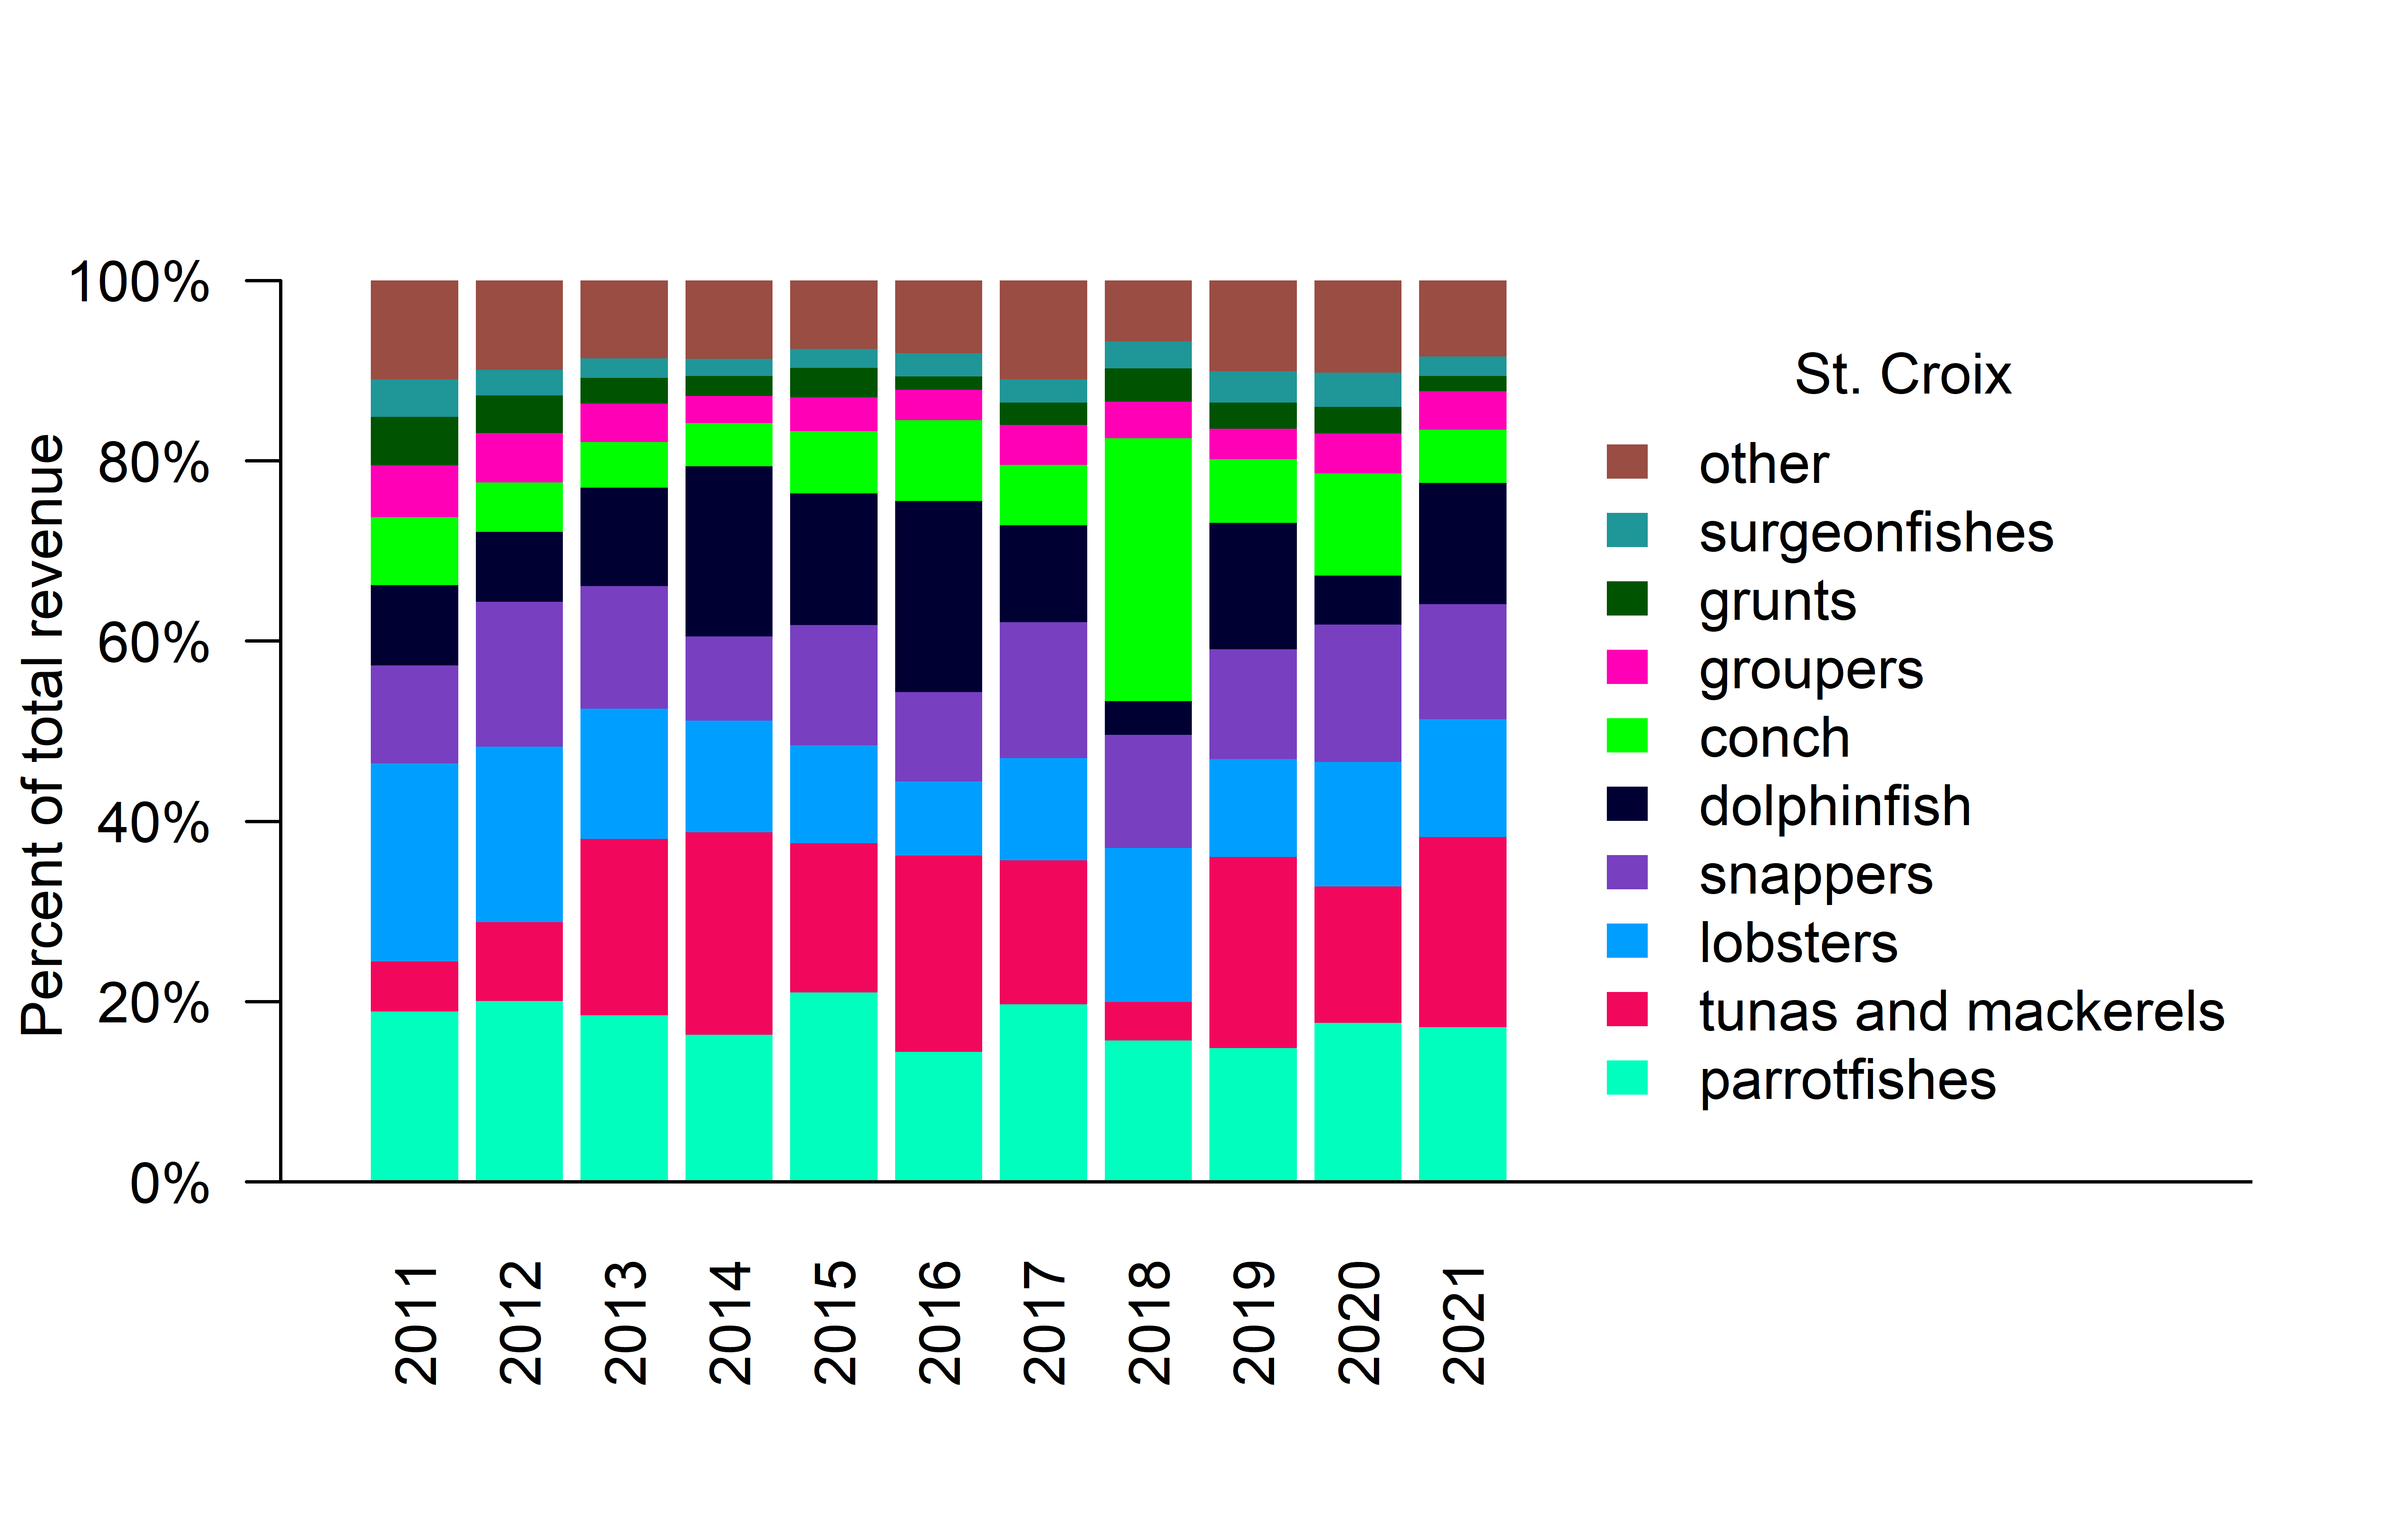
\includegraphics{indicator_plots/per_landings_STX.png}

}

\caption{\label{fig-perlandSTX}STX}

\end{figure}%

\subsection{Total, lobster and conch
trips}\label{total-lobster-and-conch-trips}

Commercial fishing trips are a useful socioeconomic indicator because
they capture the amount and type of effort which may be driven by market
factors, regulations, and costs of entering the fishery. The total
number of trips, broken down by gear type, was extracted from the
Caribbean Commercial Landings database by identifying unique trips based
on date and vessel number and extracting the primary reported gear used
for each trip. In Puerto Rico, trip numbers have generally decreased
over time, with marked decreases in 2017 and 2020; sudden changes in the
hook and line fishing in 2012 are due to changes in reporting forms
(Figure~\ref{fig-gearPR}). Effort has similarly declined in St.~Thomas
and St.~John; marked declines after 2010 are likely due to reduced
reporting (Figure~\ref{fig-gearSTT}). Similarly, in St.~Croix the number
of trips has declined, with the 2018-19 fishing season reporting
particularly low effort (Figure~\ref{fig-gearSTX}).

\begin{figure}

\centering{

\captionsetup{labelsep=none}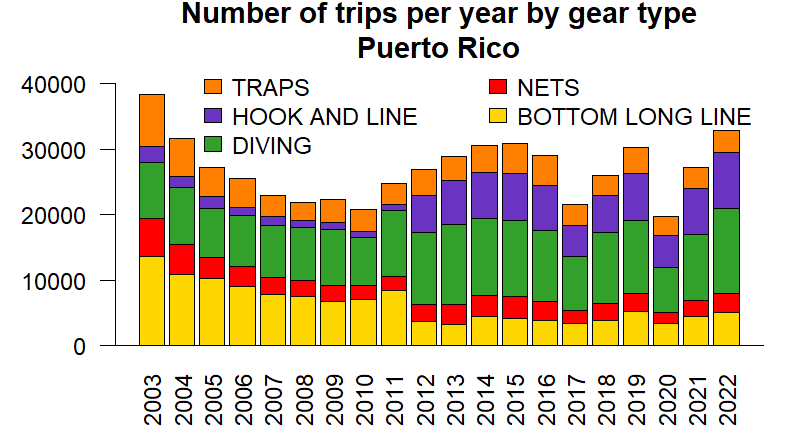
\includegraphics{indicator_plots/gearTypes_PR.png}

}

\caption{\label{fig-gearPR}}

\end{figure}%

\begin{figure}

\centering{

\captionsetup{labelsep=none}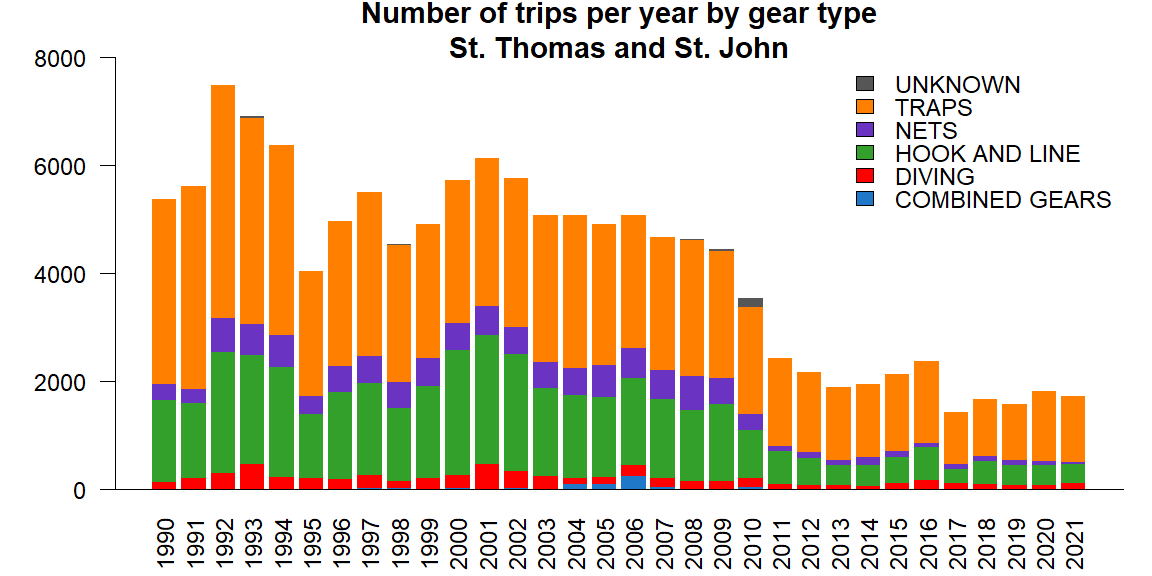
\includegraphics{indicator_plots/gearTypes_STT.png}

}

\caption{\label{fig-gearSTT}}

\end{figure}%

\begin{figure}

\centering{

\captionsetup{labelsep=none}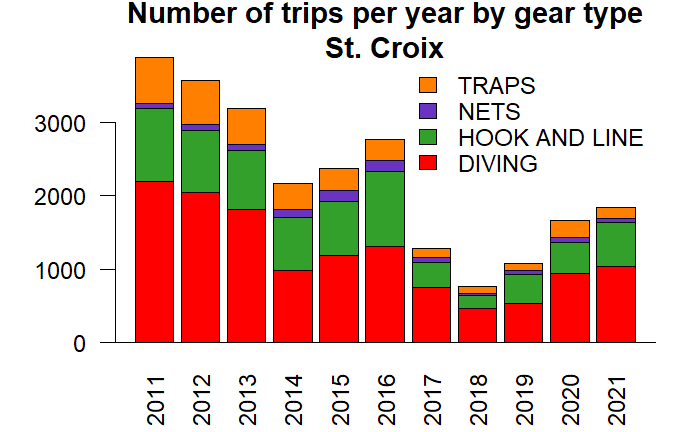
\includegraphics{indicator_plots/gearTypes_STX.png}

}

\caption{\label{fig-gearSTX}}

\end{figure}%

Given the potential for changes in reporting to impact trip numbers, it
is more informative to look at the composition of gear types. In
particular, diving is often a way of entry for new or part-time
fishermen as it generally requires lower up-front investments. Peaks in
the proportion diving trips in 2017 and 2018 could be a result of lost
traps and infrastructure due to hurricanes (Figure~\ref{fig-dive}).

\begin{figure}

\centering{

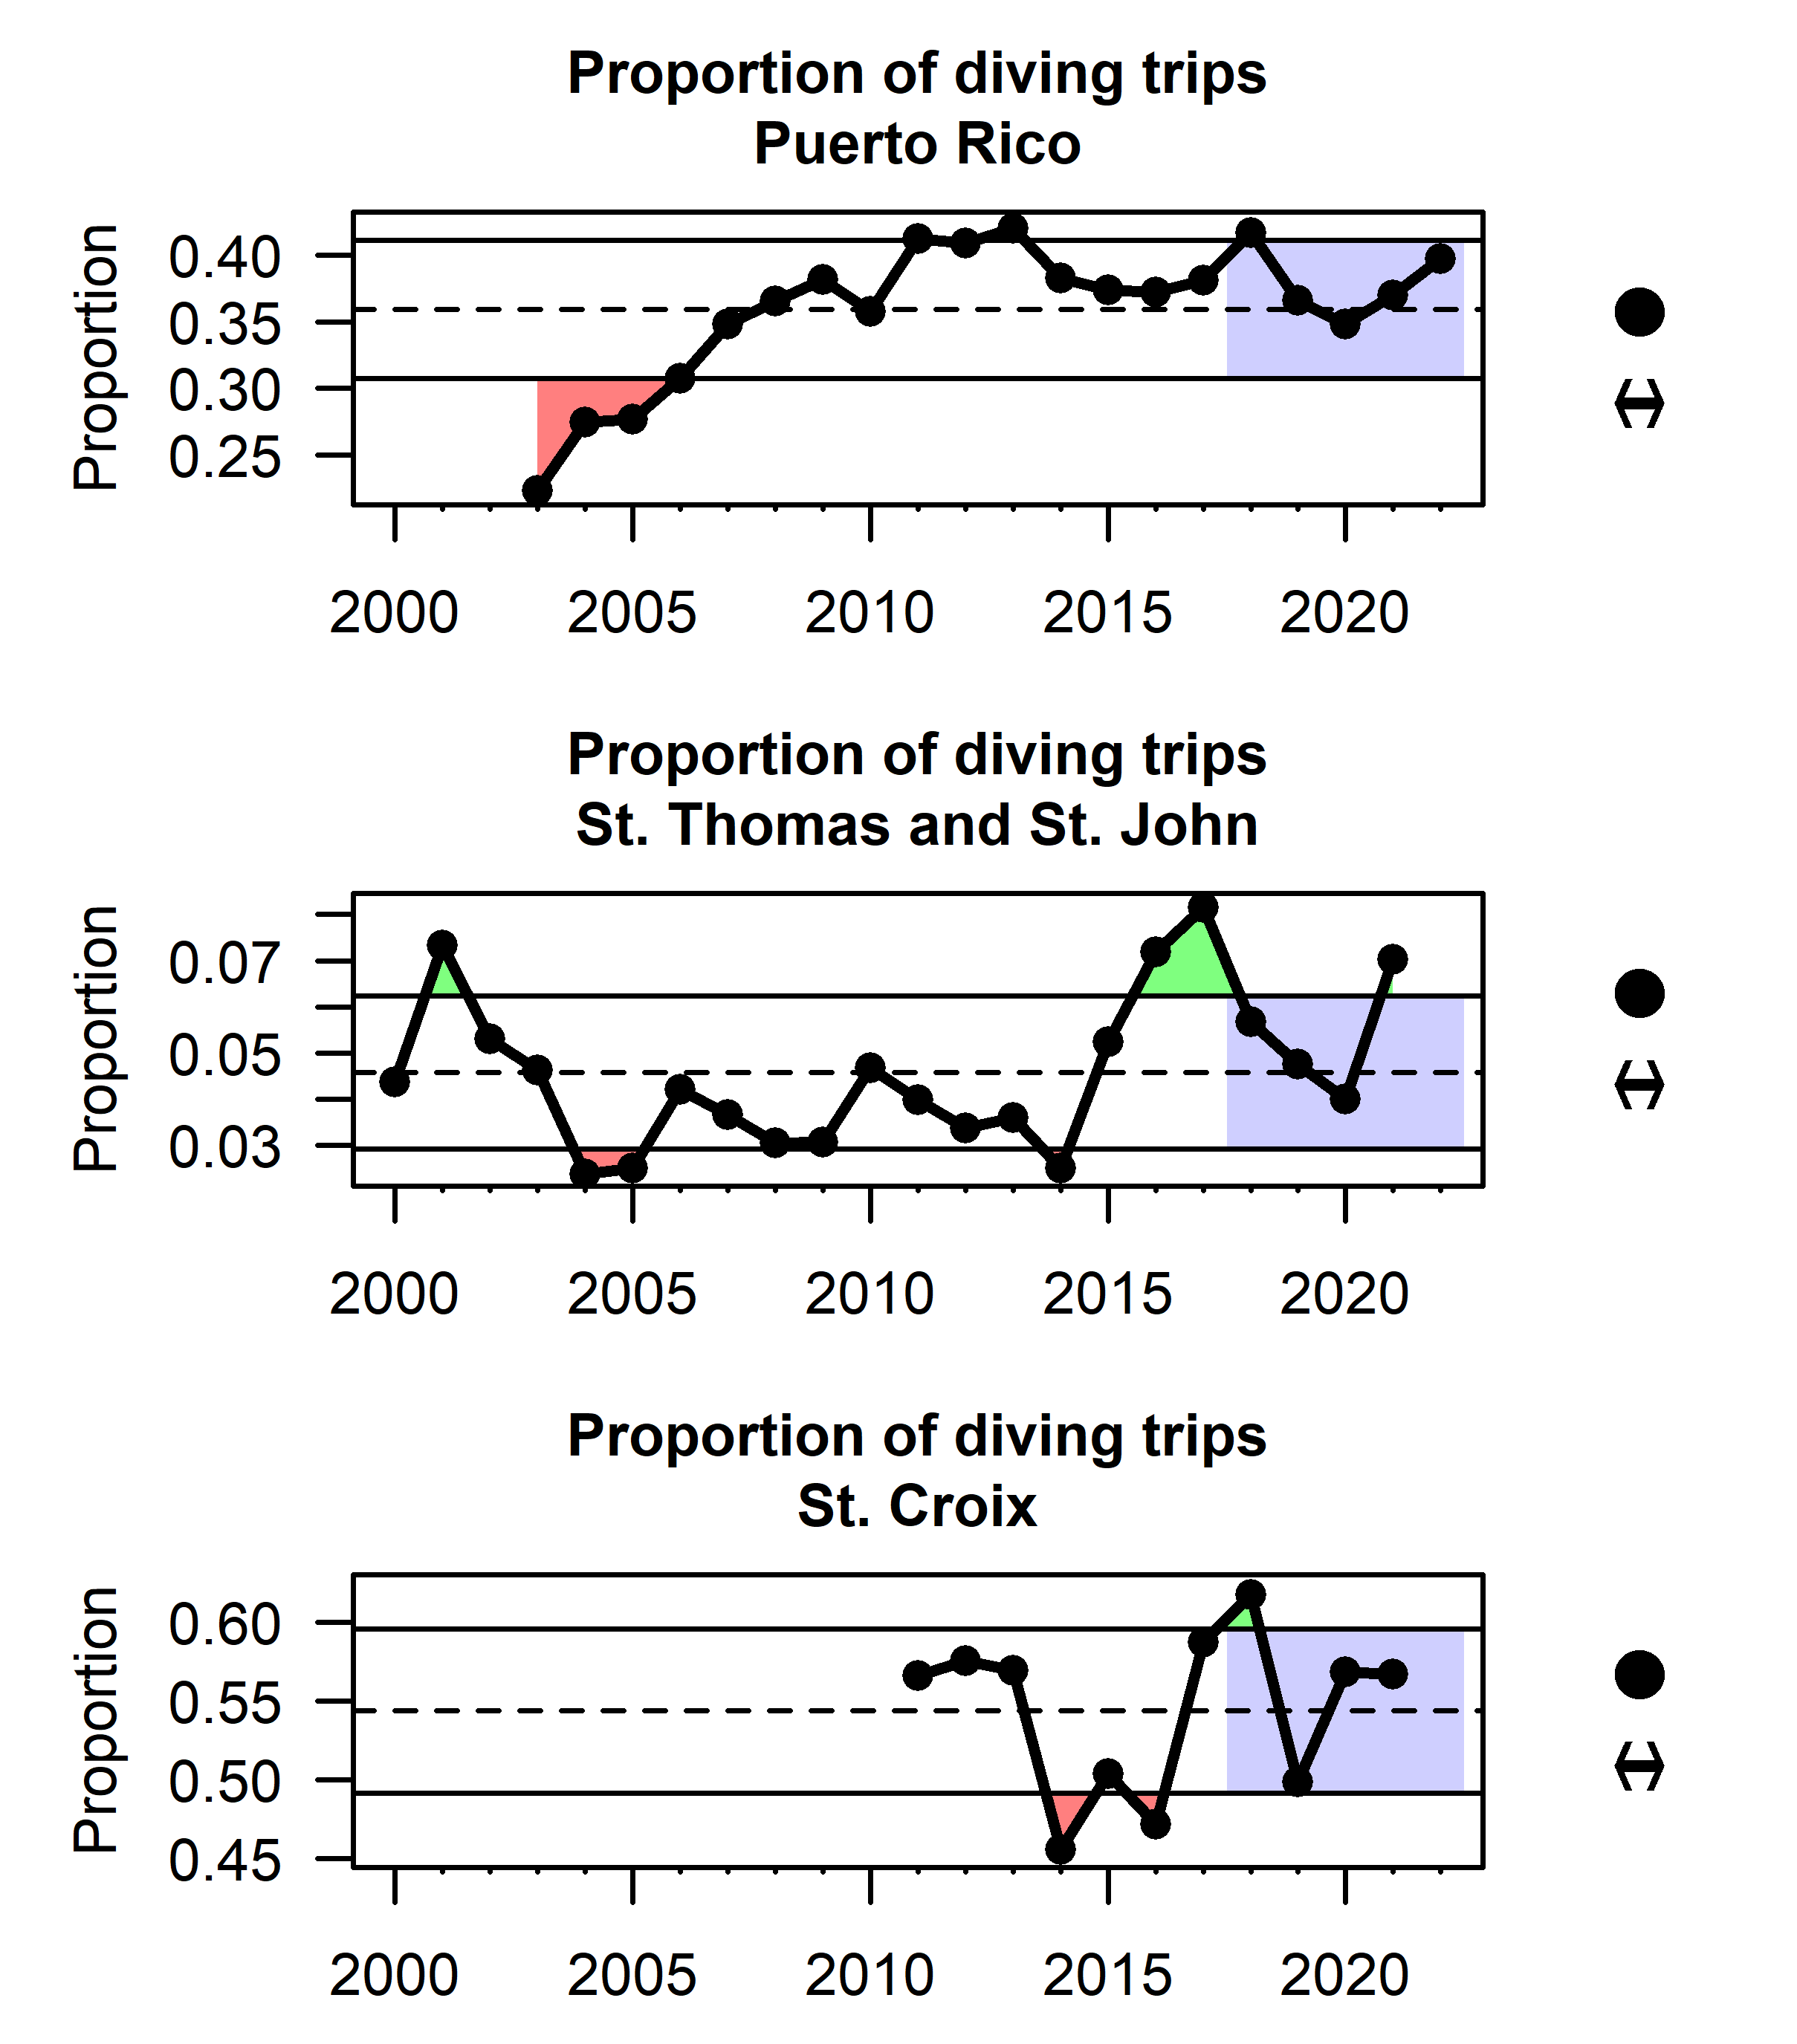
\includegraphics{indicator_plots/prop_diving_trips_plot_final.png}

}

\caption{\label{fig-dive}Diving trips}

\end{figure}%

Ordination of gear types based on reporting landing sites conveys how
different regions across the U.S. Caribbean depend on different methods
of fishing. Ordinations were conducting using NMDS based on matrices
representing the proportion of gears used by landing site; the algorithm
seeks to place different sites in an X-dimensional space, such that the
physical distances between each pair of sites best represents the
differences in gear types employed. Thus, sites that appear more closely
together in the figures are more similar in their gear usage, and the
position of the gear type labels denote the relative importance of those
gears in those sites. In Puerto Rico for example, hook and line and
bottom long line are closely related and are particularly prevalent in
the northern landing sites (in red), whereas nets and traps are more
prevalent in the South (blue) (Figure~\ref{fig-NMDSPR}). In St.~Thomas
and St.~John, there is an association of traps and hook and line fishing
(Figure~\ref{fig-NMDSSTT}), whereas in St.~Croix, those gears are not
associated with each other but nets and spearfishing are closely
associated within landing sites (Figure~\ref{fig-NMDSSTX}).

\begin{figure}

\centering{

\captionsetup{labelsep=none}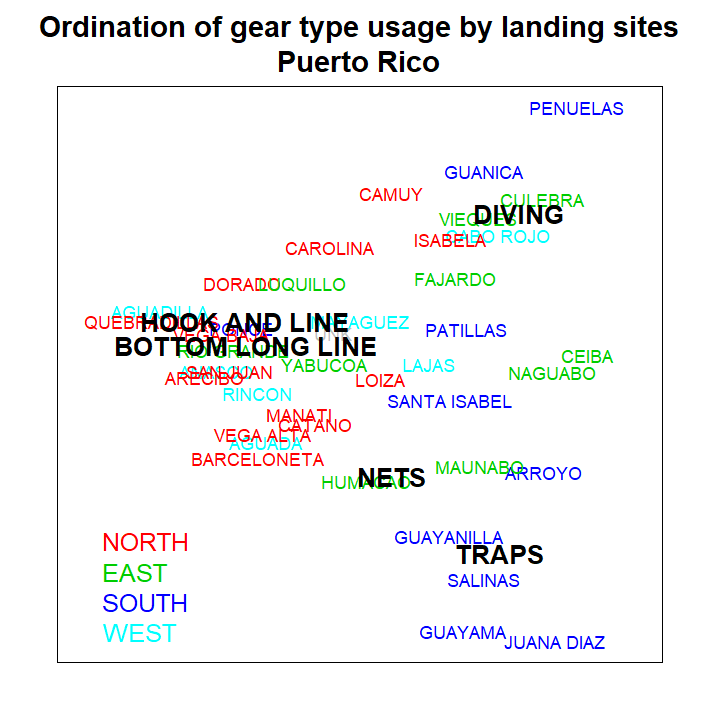
\includegraphics{indicator_plots/NMDSgear_PR.png}

}

\caption{\label{fig-NMDSPR}}

\end{figure}%

\begin{figure}

\centering{

\captionsetup{labelsep=none}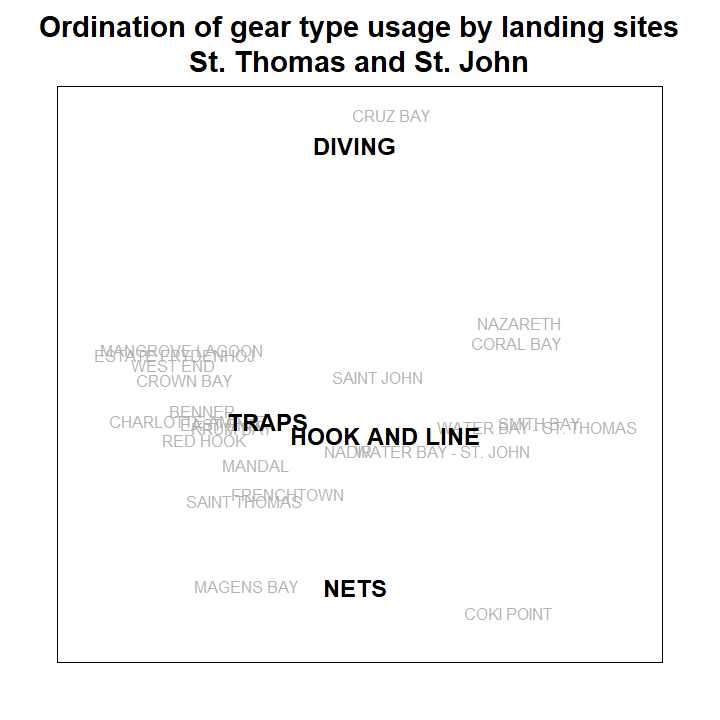
\includegraphics{indicator_plots/NMDSgear_STT.png}

}

\caption{\label{fig-NMDSSTT}}

\end{figure}%

\begin{figure}

\centering{

\captionsetup{labelsep=none}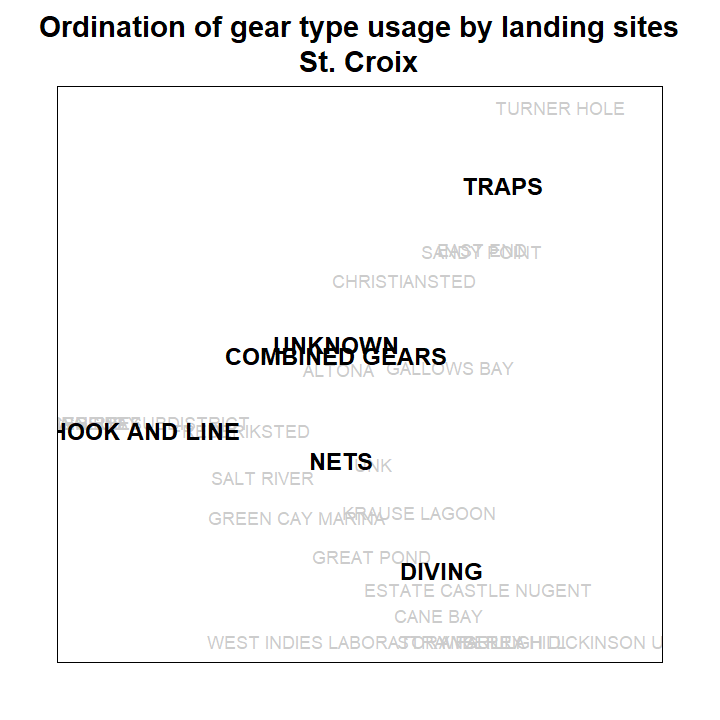
\includegraphics{indicator_plots/NMDSgear_STX.png}

}

\caption{\label{fig-NMDSSTX}}

\end{figure}%

\subsection{Economic activity}\label{economic-activity}

Some high level indicators of economic activity come in the form of GDP
and employment trends. Gross Domestic Product (GDP) data come from the
Bureau of Economic Analysis (BEA), and indicate an overall general
economic expansion in Puerto Rico. GDP in USVI declined substantially
from 2007-2014, but has been increasing steadily since
(Figure~\ref{fig-GDP}).

\begin{figure}

\centering{

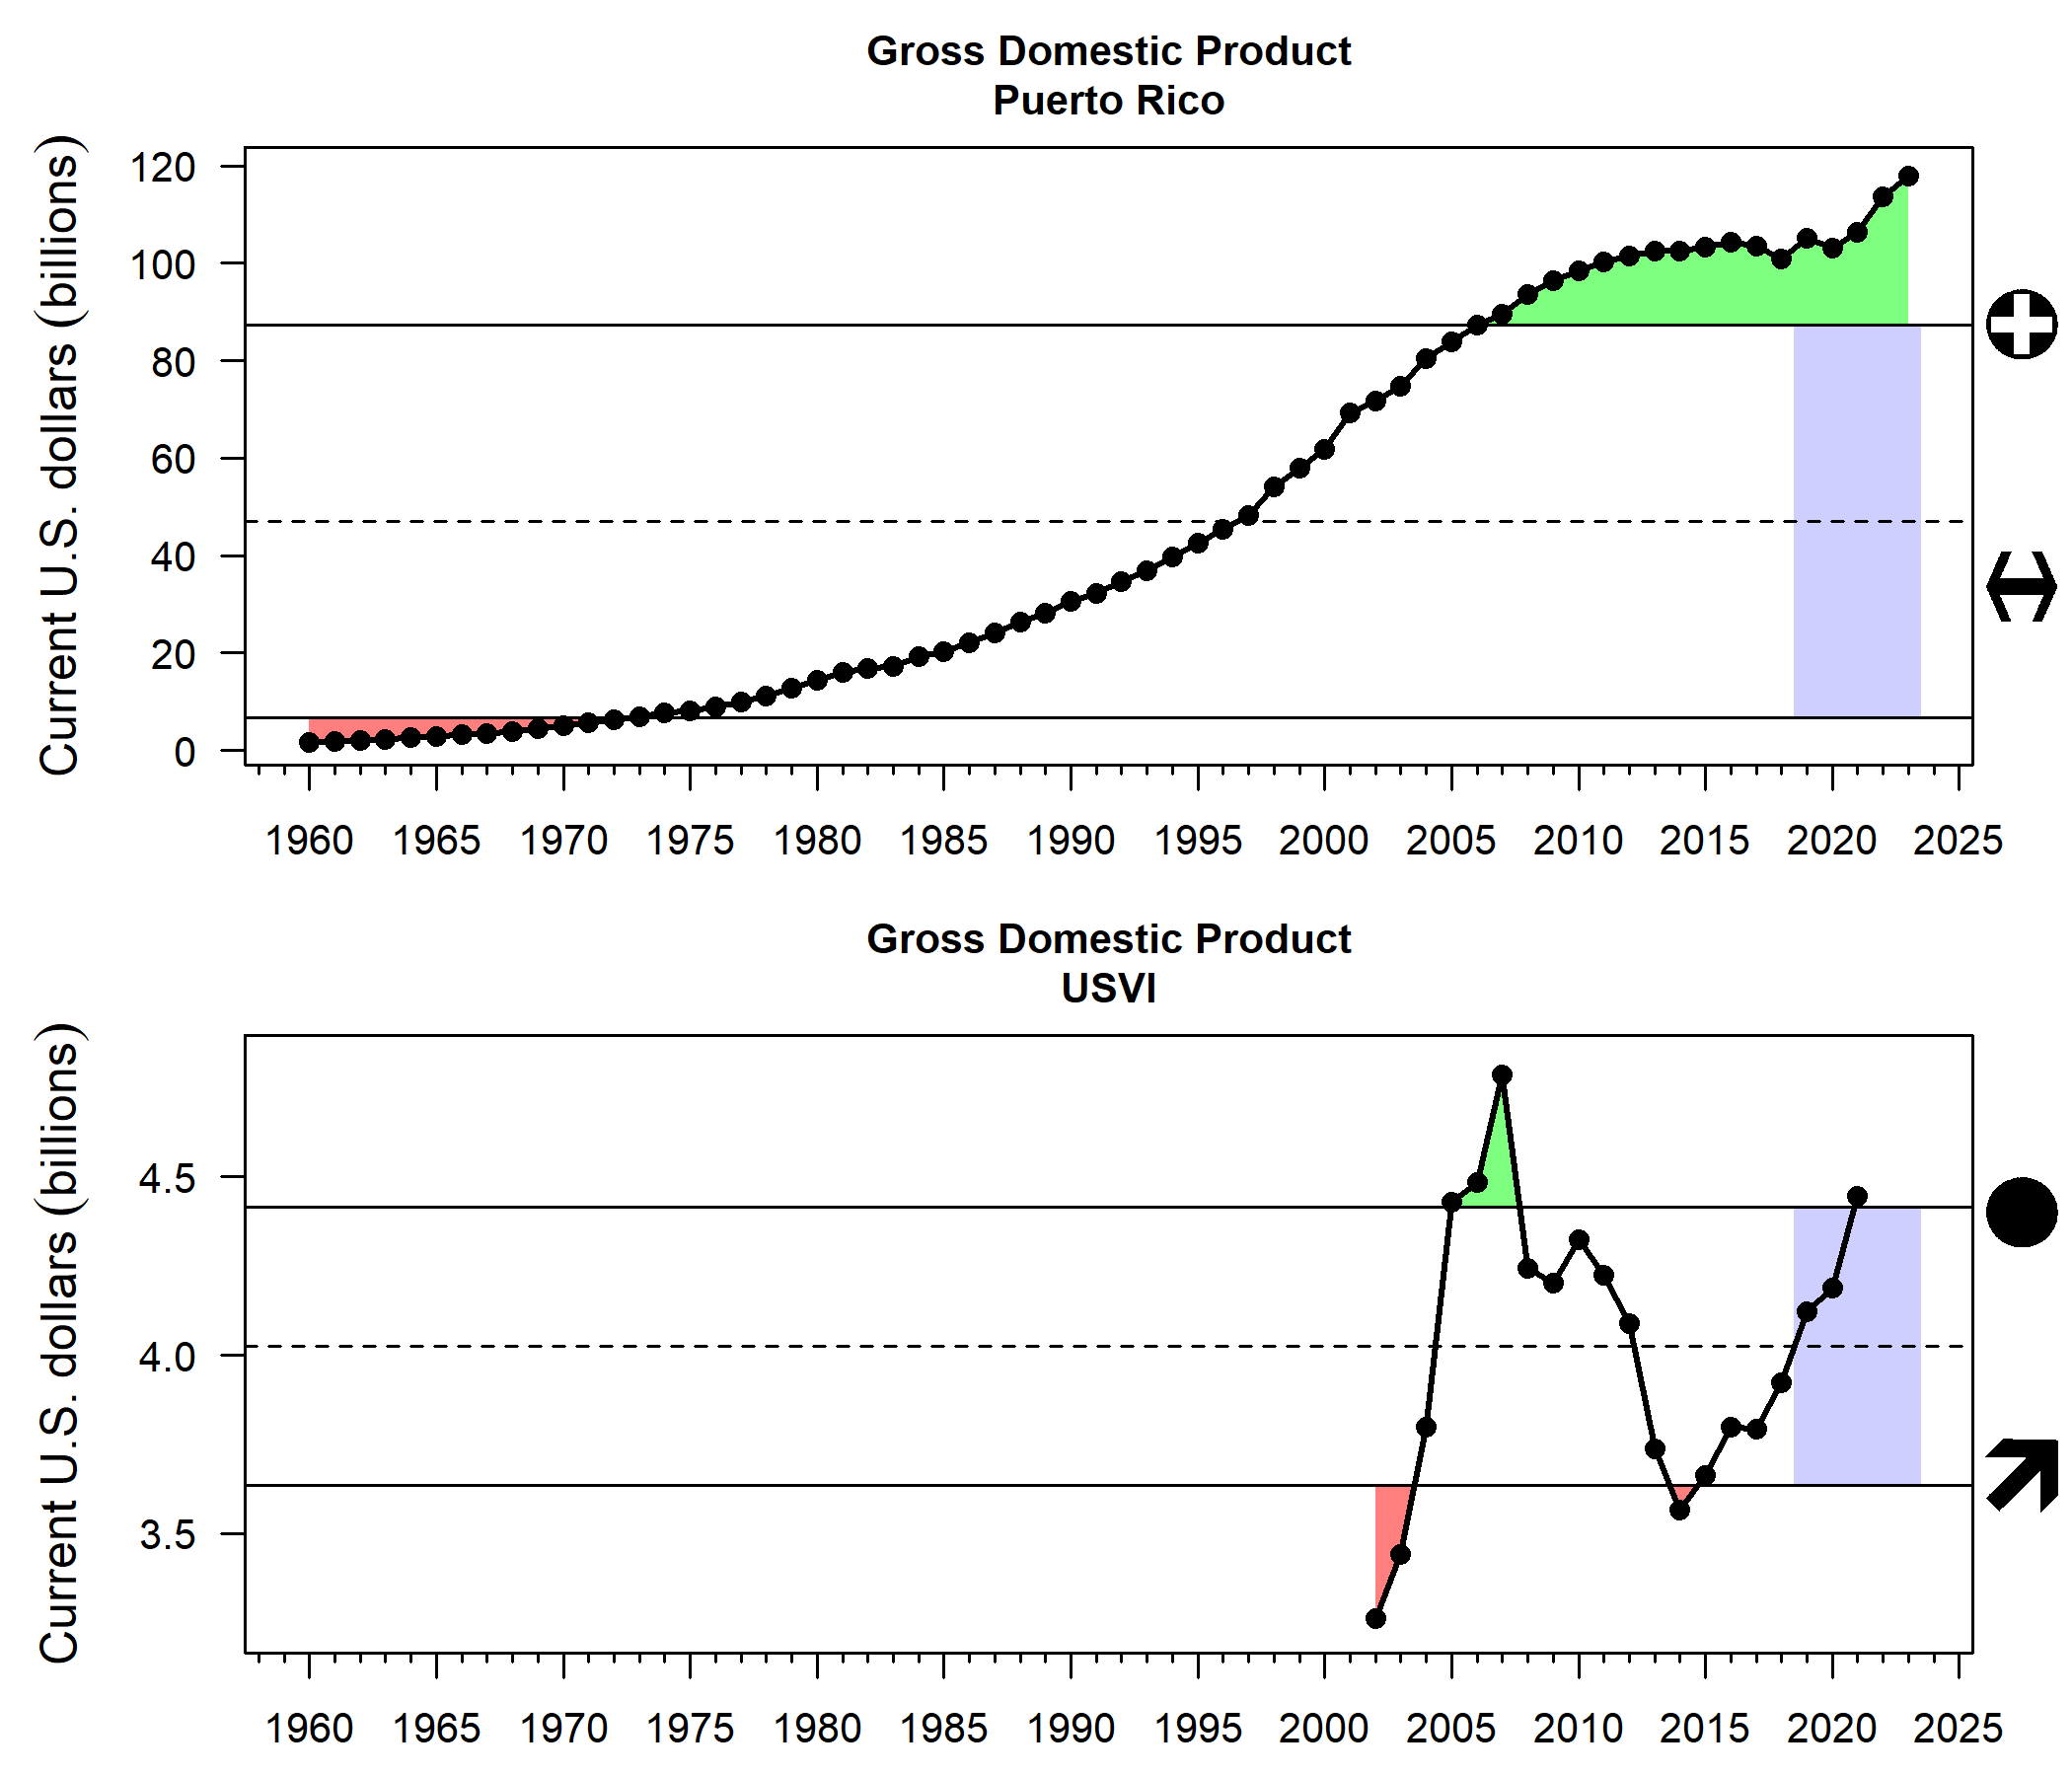
\includegraphics{indicator_plots/GDP_plot_final.png}

}

\caption{\label{fig-GDP}GDP}

\end{figure}%

GDP can sometimes underestimate the ocean-dependency of the regions'
local island economies; another indicator that is useful is
employment/unemployment rate data, which come from the USVI Bureau of
Economic Research.

\begin{figure}

\centering{

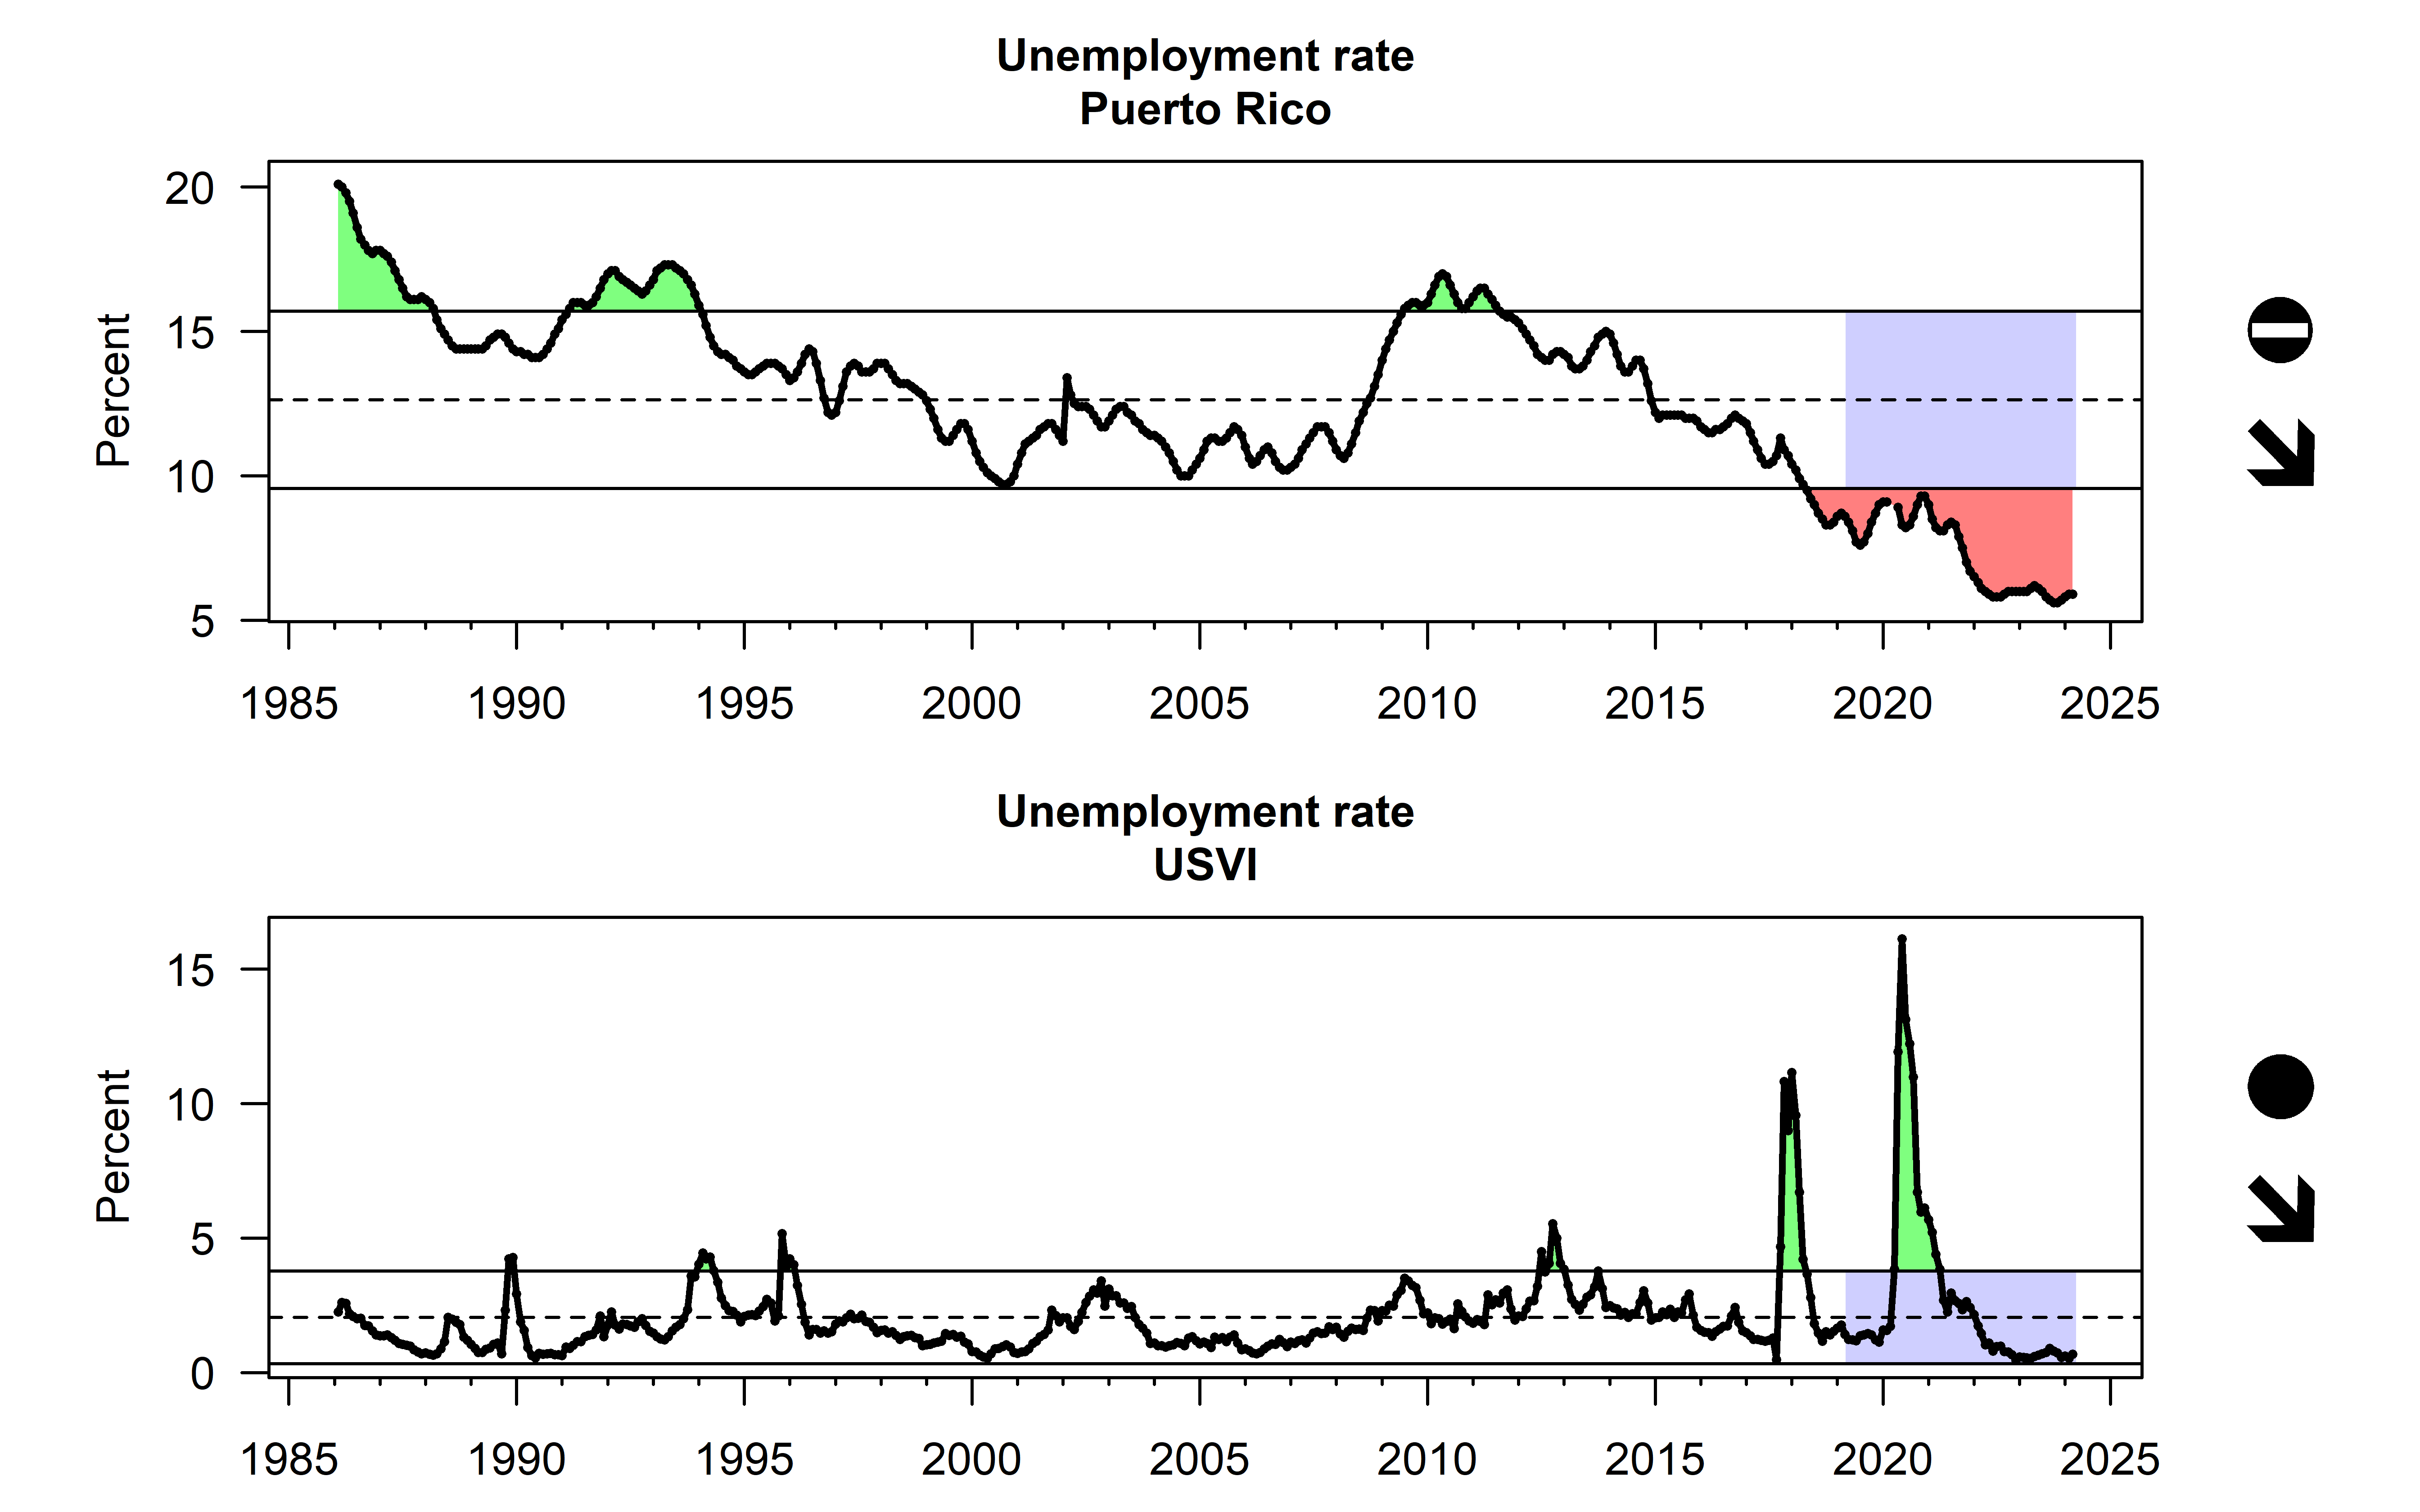
\includegraphics{indicator_plots/unemployment_plot_final.png}

}

\caption{\label{fig-unemp}Unemployment}

\end{figure}%

\subsection{Ocean economy establishments, employment, and
wages}\label{ocean-economy-establishments-employment-and-wages}

Due to their unique geography, culture and setting, the islands of
Puerto Rico and the U.S. Virgin Islands are more reliant on the
surrounding ocean and marine environments than the continental United
States. Data from the Bureau of Labor Statistics Quarterly Census of
Employment and Wages
(https://www.bls.gov/cew/downloadable-data-files.htm) provides data on
the number of establishments, employees, and wages earned for each
county by industry (as defined by NAICS code). These data underpin the
Economics: National Ocean Watch (ENOW) methods created by NOAA OCM to
track contributions of the ocean economy to the overall economy, however
must be taken in their raw form for the US territories because overall
GDP is not calculated in the territories. We used the NAICS codes
defined by the ENOW program as contributing to the ocean economy
(citation: https://coast.noaa.gov/data/digitalcoast/pdf/enow-faq.pdf).
The NAICS classification system has changed through time, with notable
updates in 2007, 2011, and 2017 (citation:
https://www.bls.gov/cew/classifications/industry/home.htm) -- note the
large increase in ocean economic activity in both areas associated with
the 2011 update. Otherwise, employment and wages in both Puerto Rico and
the USVI are relatively stable through time (Figure~\ref{fig-NAICS}).

\begin{figure}

\centering{

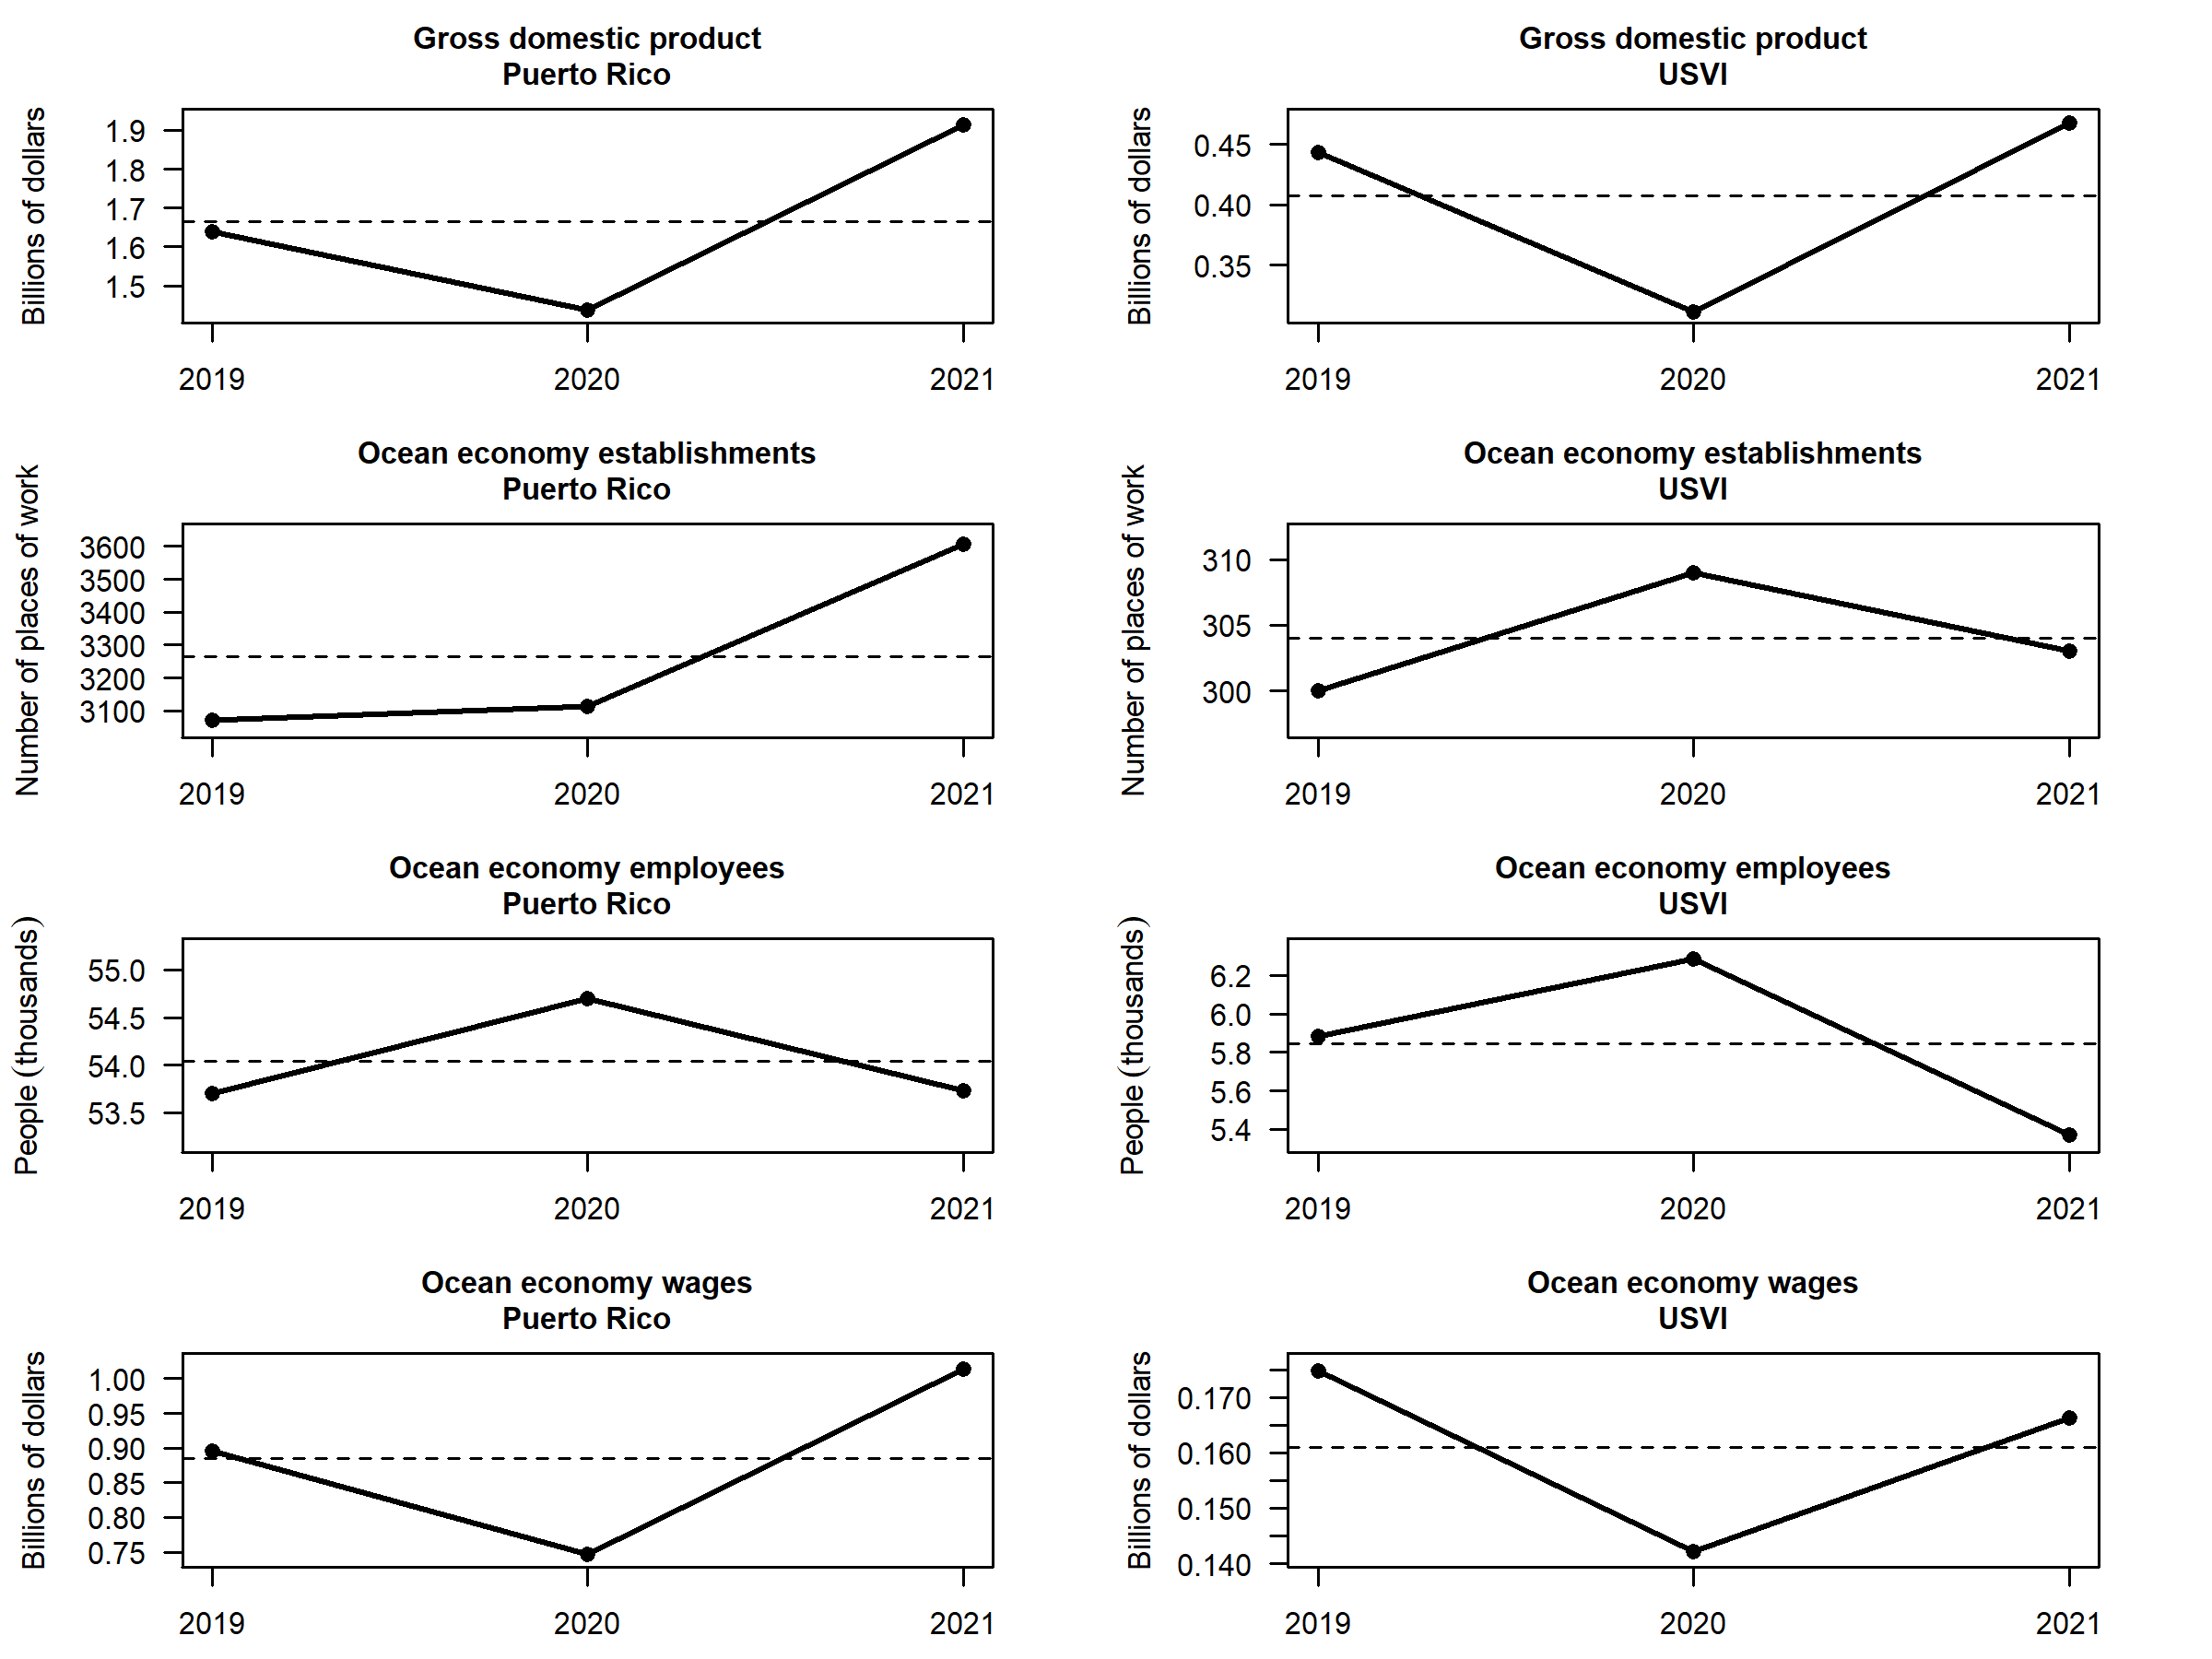
\includegraphics{indicator_plots/oceanNAICS_plot_final.png}

}

\caption{\label{fig-NAICS}Ocean economy}

\end{figure}%

\section{Equity}\label{equity}

\subsection{Gini coefficient for distribution of landings and
revenue}\label{gini-coefficient-for-distribution-of-landings-and-revenue}

Equality in the distribution of revenues across the fishery can be
represented by the Gini index which is a value ranging from zero to one,
with zero representing perfect equality (revenues distributed equally
among all participants) and a value of one representing maximum
inequality (all revenues going to a single individual, Gini 1936). The
Gini index was calculated based on reported revenues from the Caribbean
Commercial Landings database, as they are distributed across the
individual vessel or fisher permits (Figure~\ref{fig-gini}). Overall,
the Gini index values suggest that consolidation across U.S. Caribbean
fisheries is high compared to other U.S. regions, though this may be an
artifact of reporting if more experienced fishermen are more frequently
reporting. In St.~Thomas/St.~John, the index shows a gradual increase
throughout the time period, while there is no particular trend apparent
in Puerto Rico and St.~Croix. There are spikes in inequality in Puerto
Rico in 2018 and in St.~Croix in 2017-2018 which may be related to
fishing industry impacts from hurricanes.

\begin{figure}

\centering{

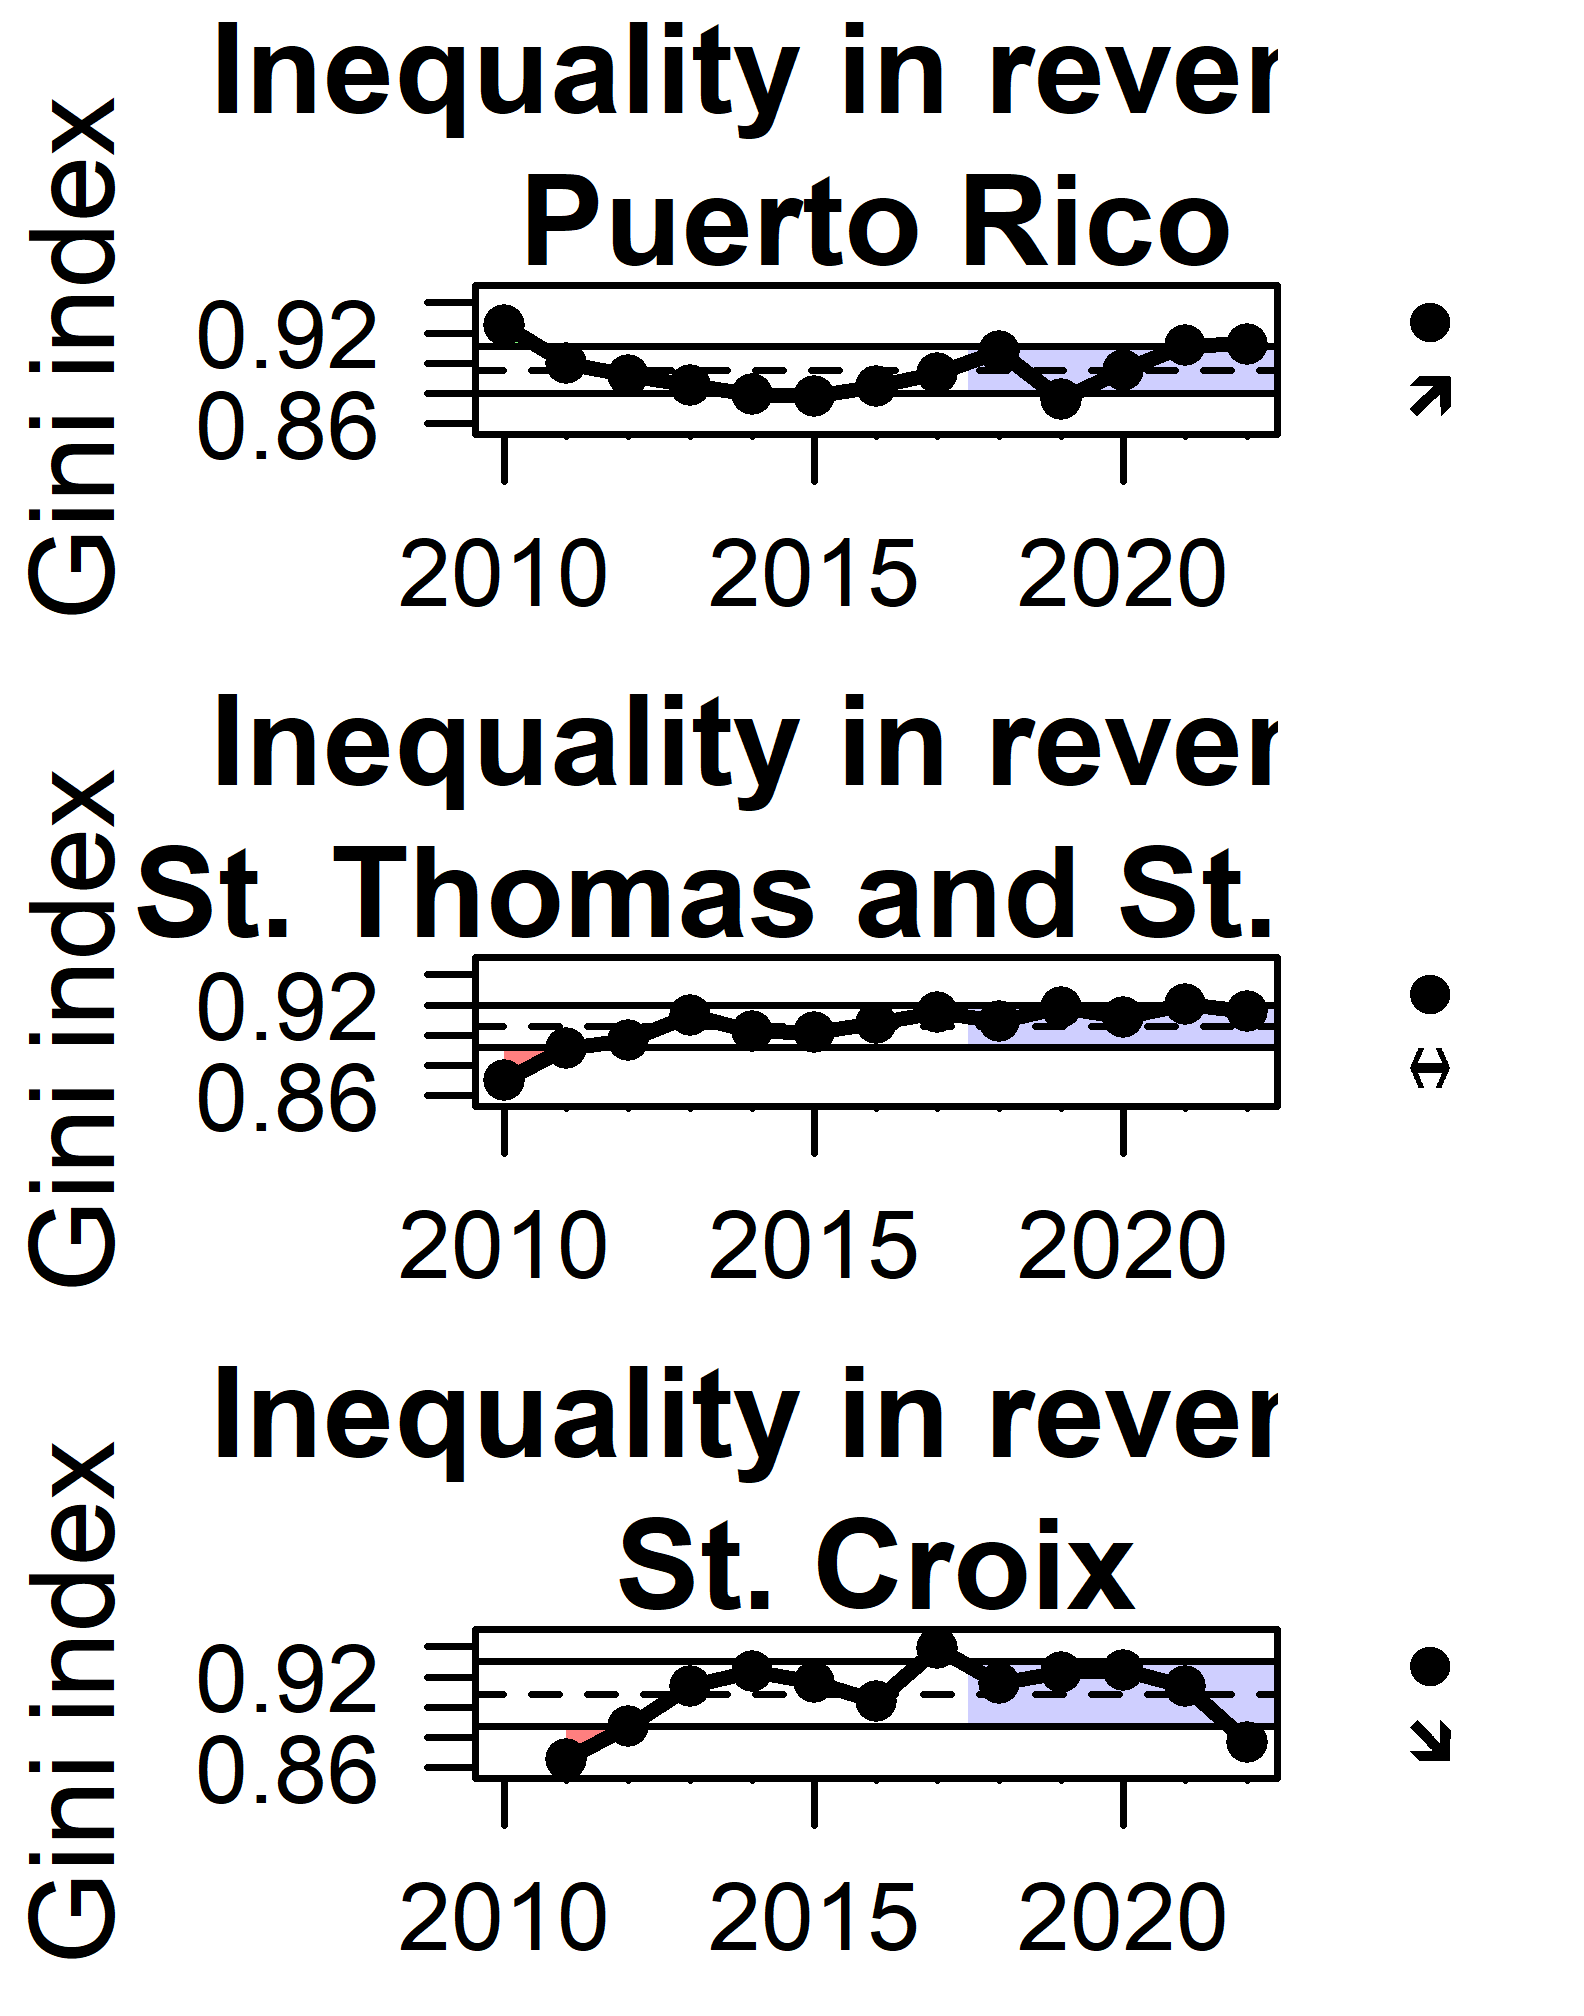
\includegraphics{indicator_plots/gini_plot_final.png}

}

\caption{\label{fig-gini}Gini coefficient}

\end{figure}%

\subsection{Environmental justice, economic, and gentrification
pressure}\label{environmental-justice-economic-and-gentrification-pressure}

Indicator 26

\begin{figure}

\centering{

\captionsetup{labelsep=none}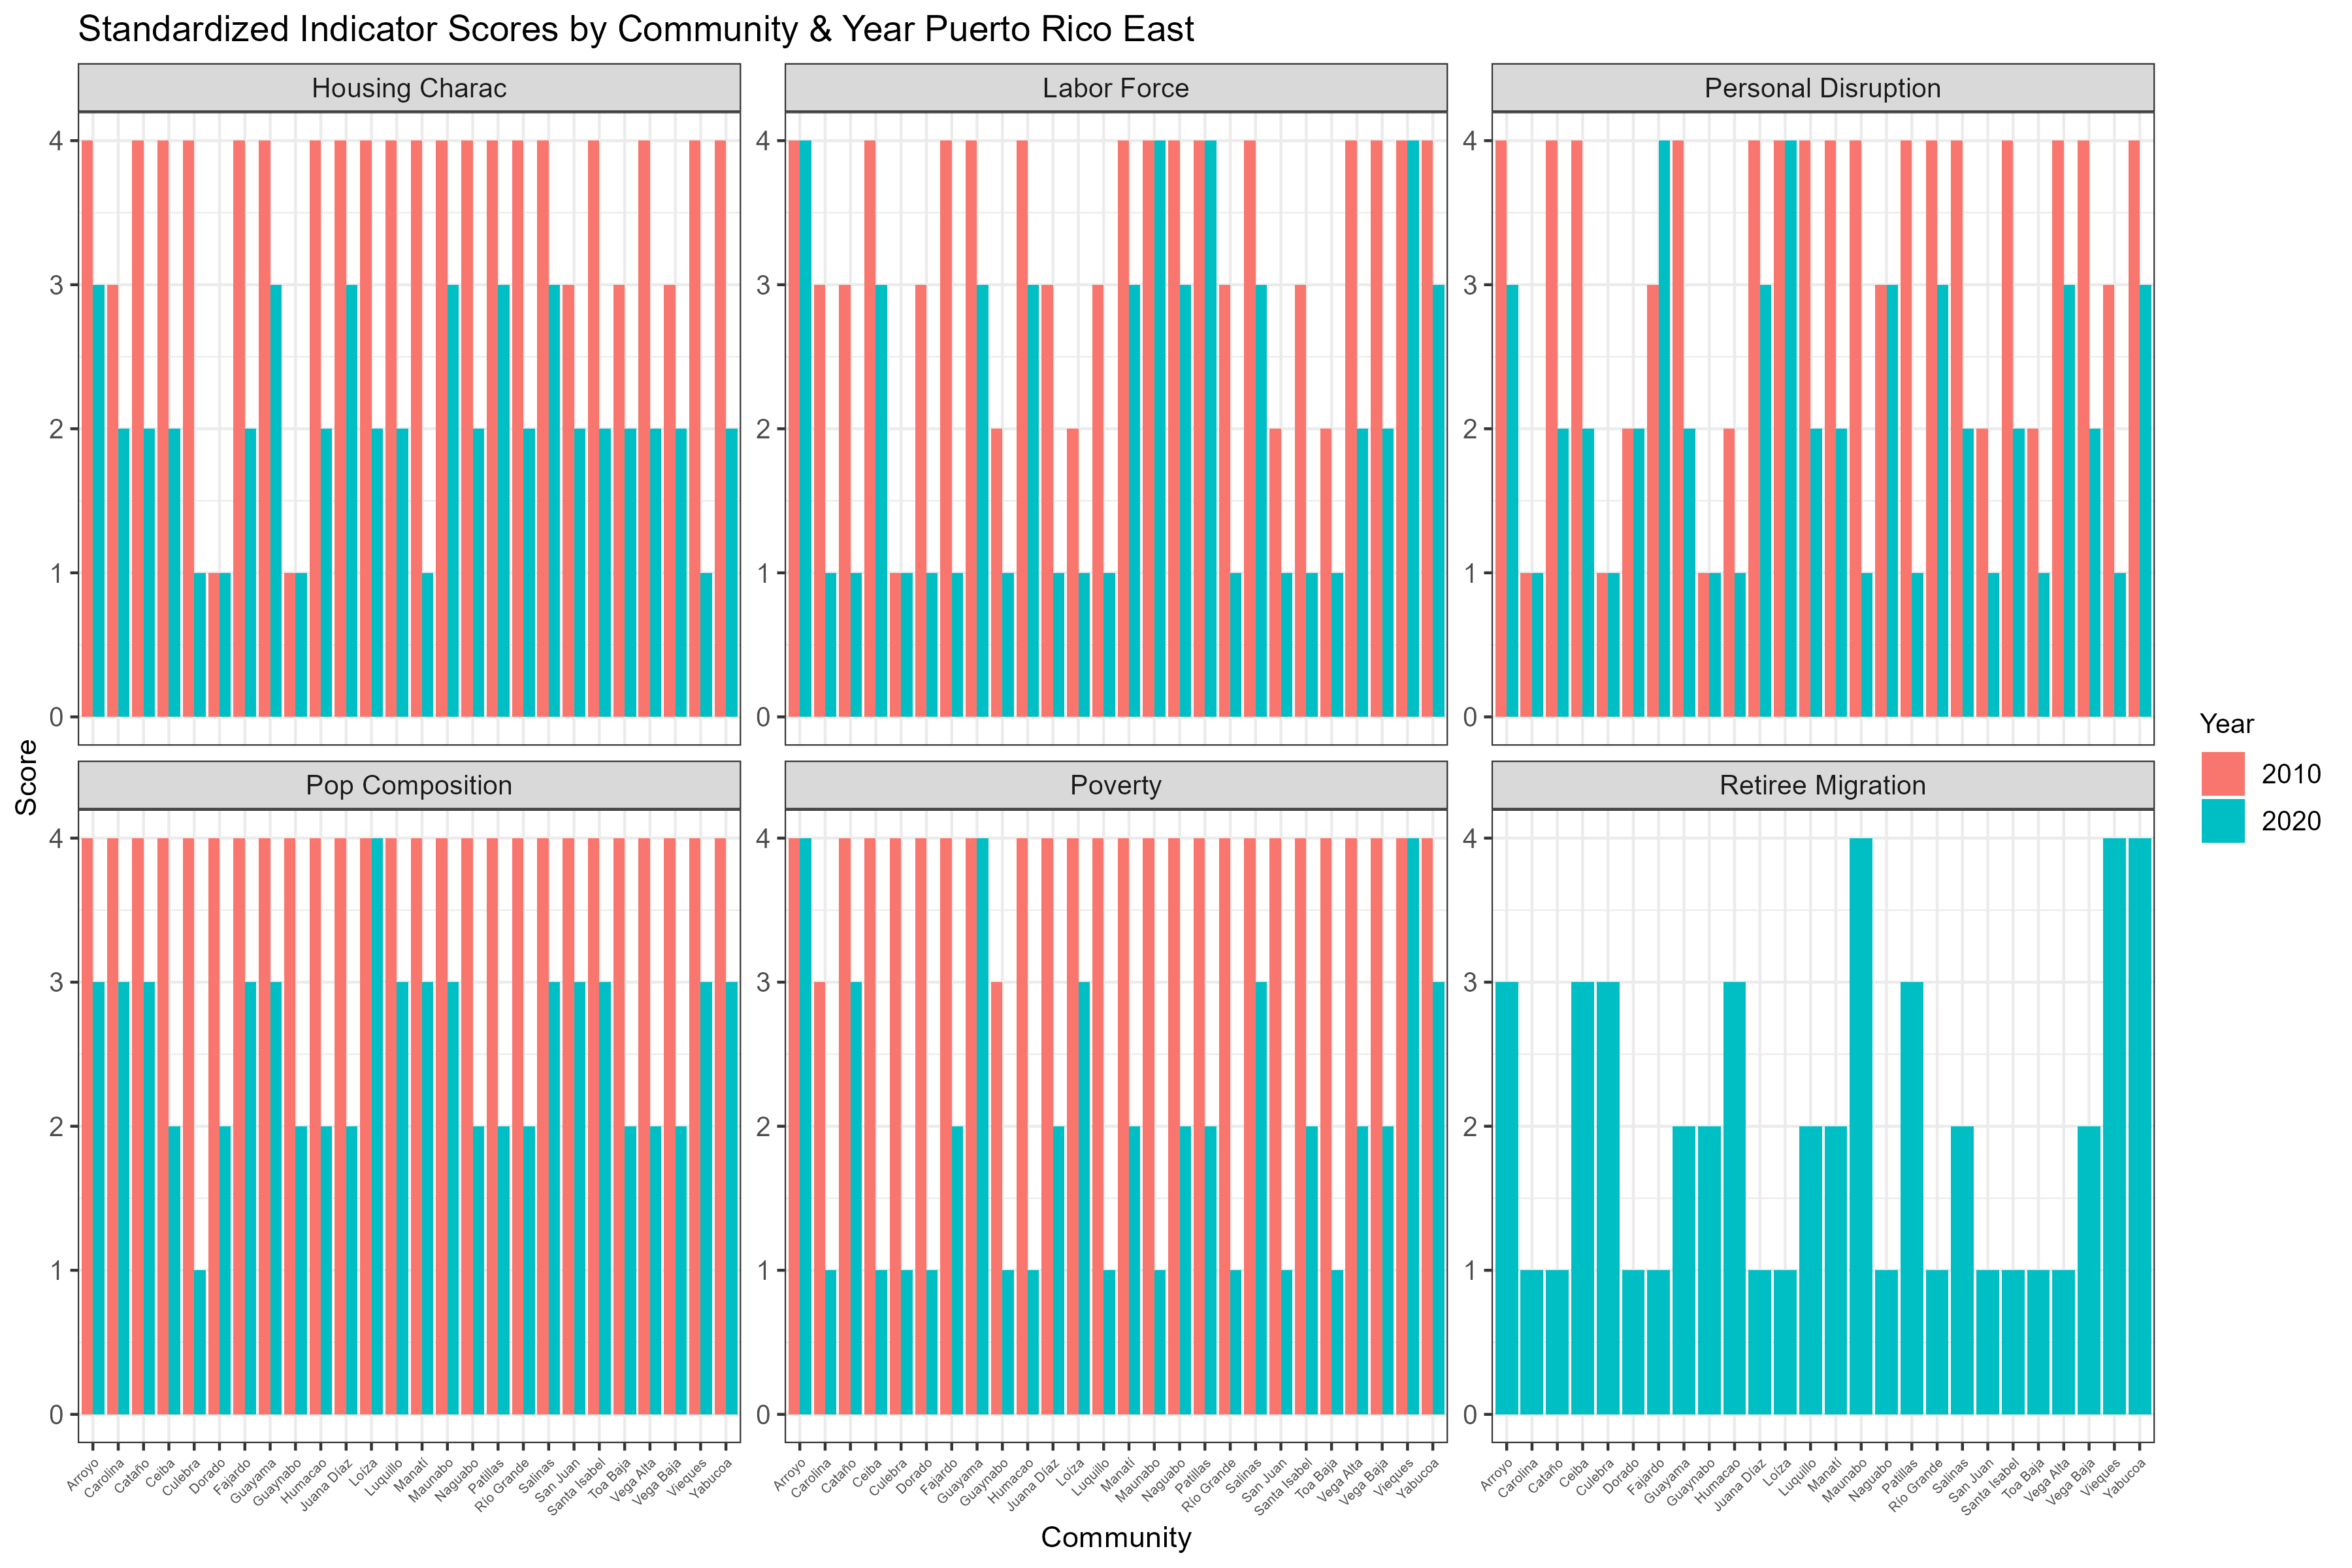
\includegraphics{indicator_plots/CSVI_plots/Faceted_Bar_Plot_Puerto Rico East.png}

}

\caption{\label{fig-CSVIPRE}}

\end{figure}%

\begin{figure}

\centering{

\captionsetup{labelsep=none}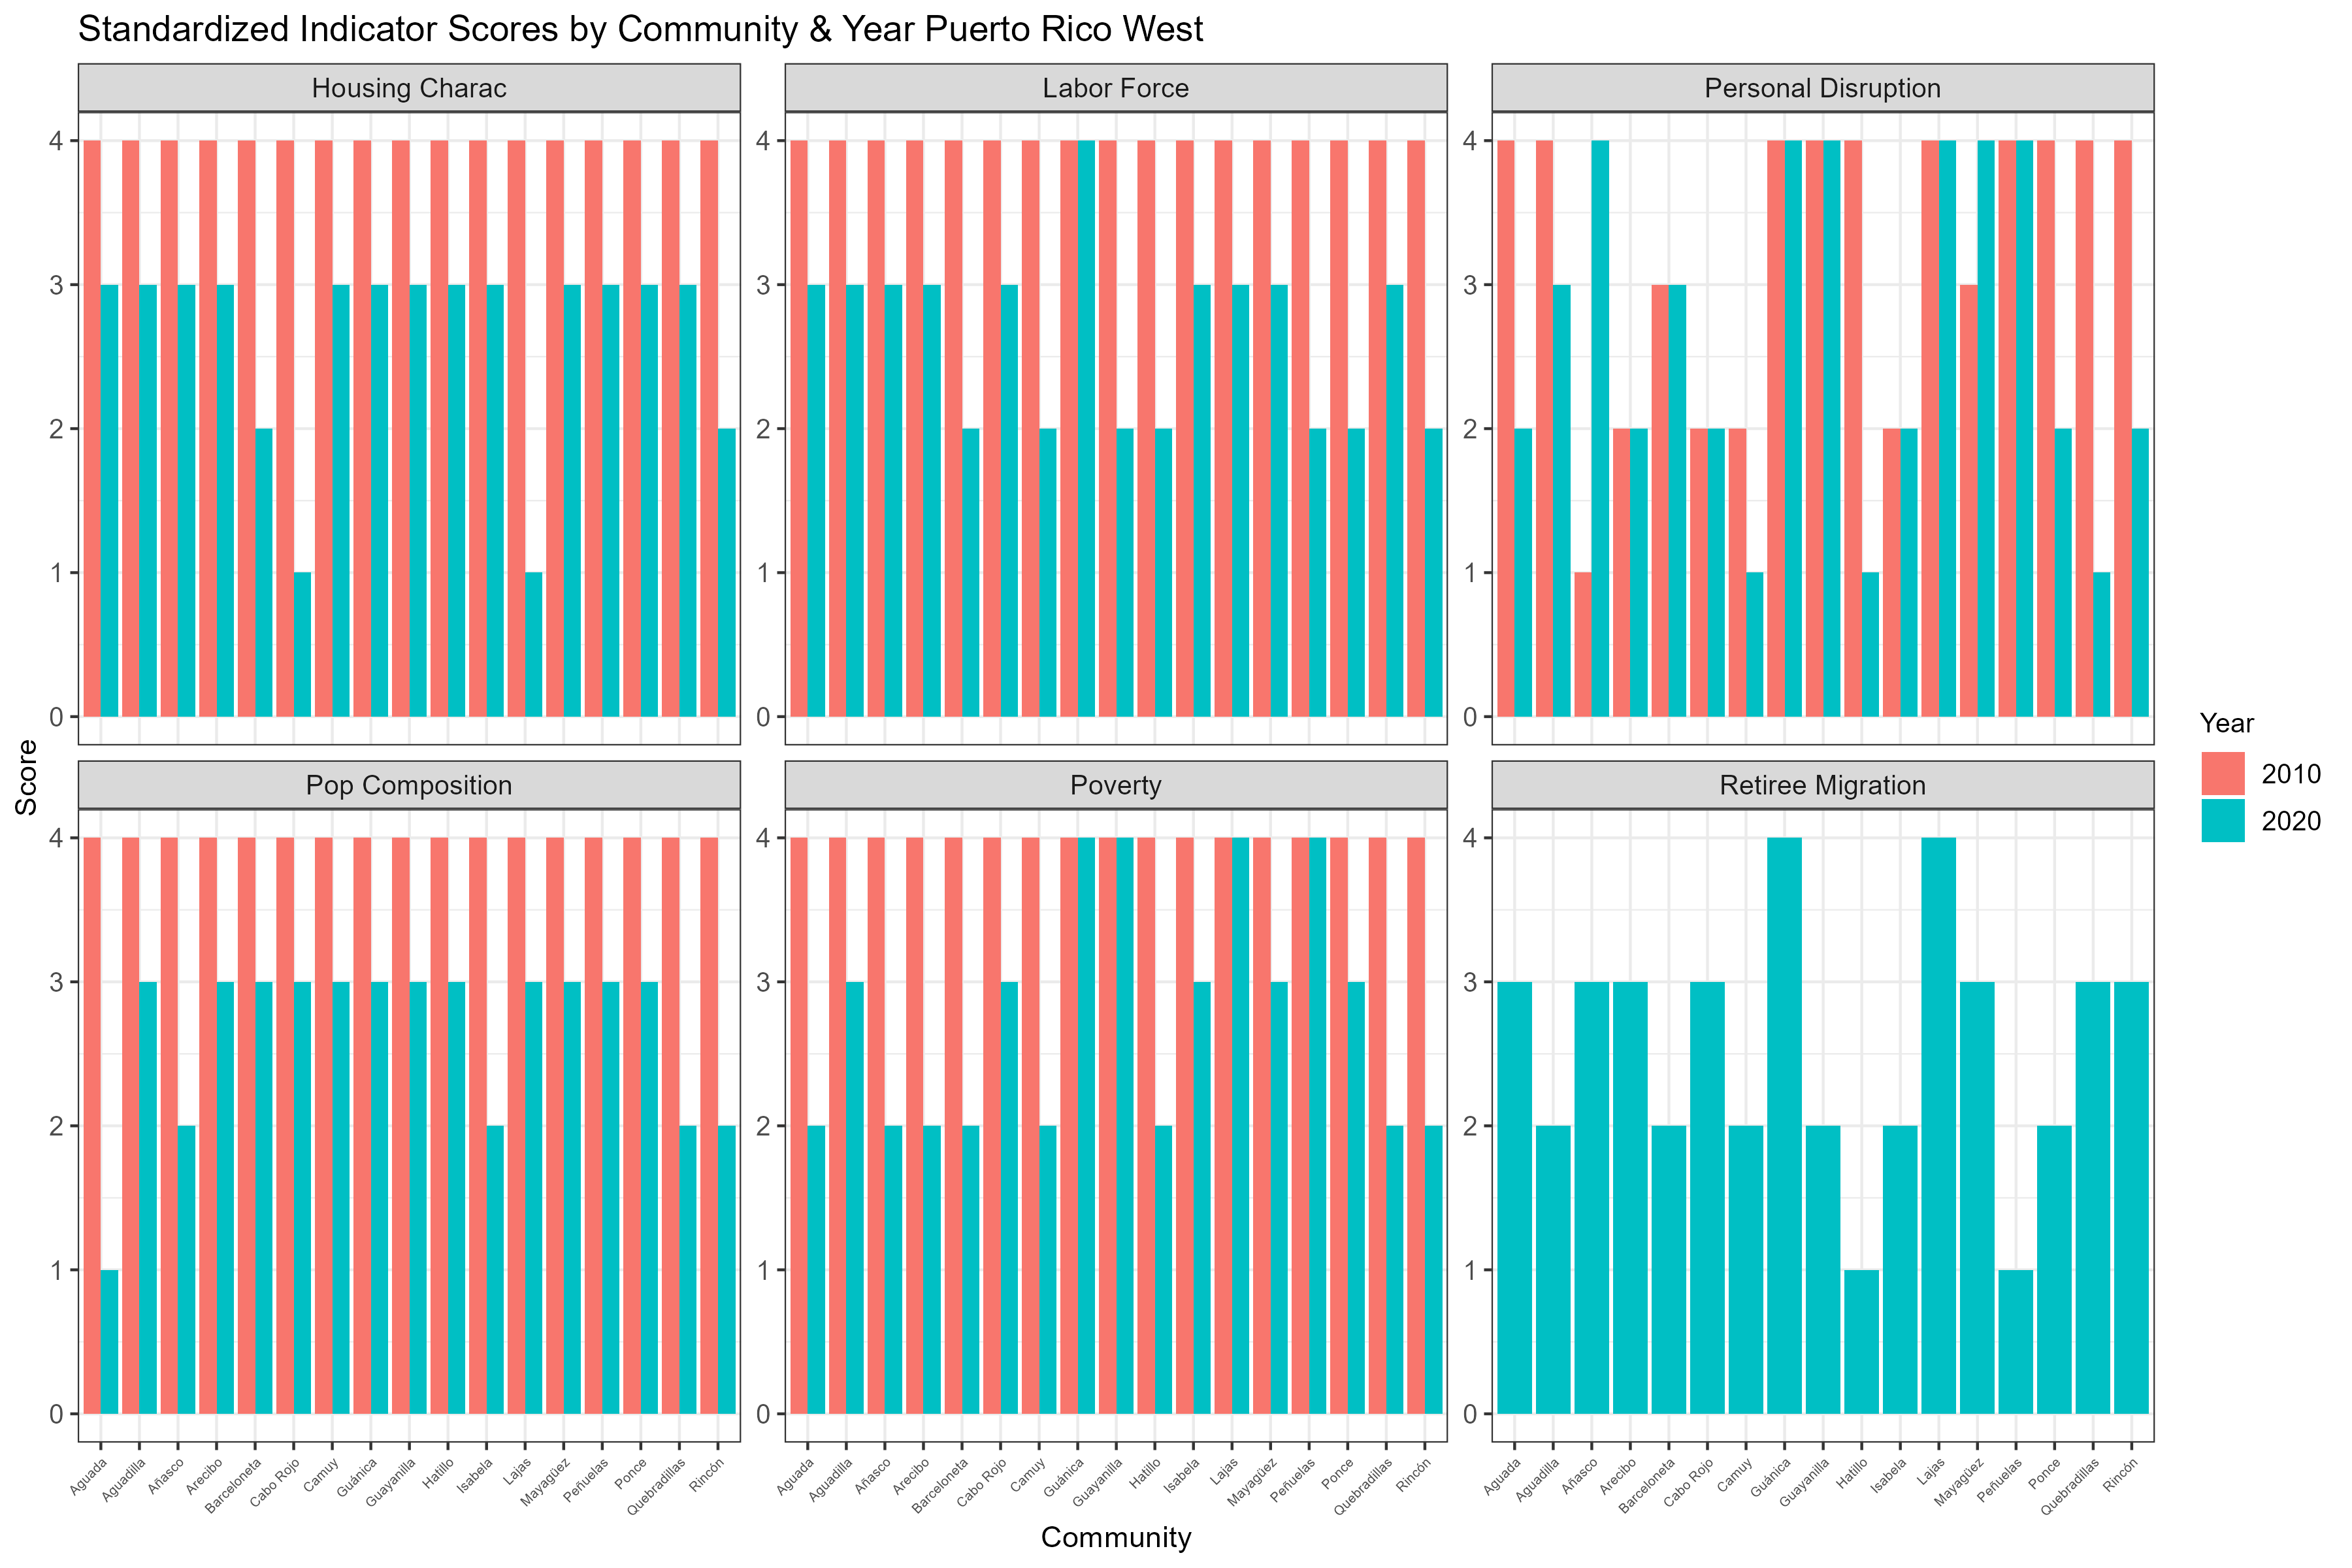
\includegraphics{indicator_plots/CSVI_plots/Faceted_Bar_Plot_Puerto Rico West.png}

}

\caption{\label{fig-CSVIPRW}}

\end{figure}%

\begin{figure}

\centering{

\captionsetup{labelsep=none}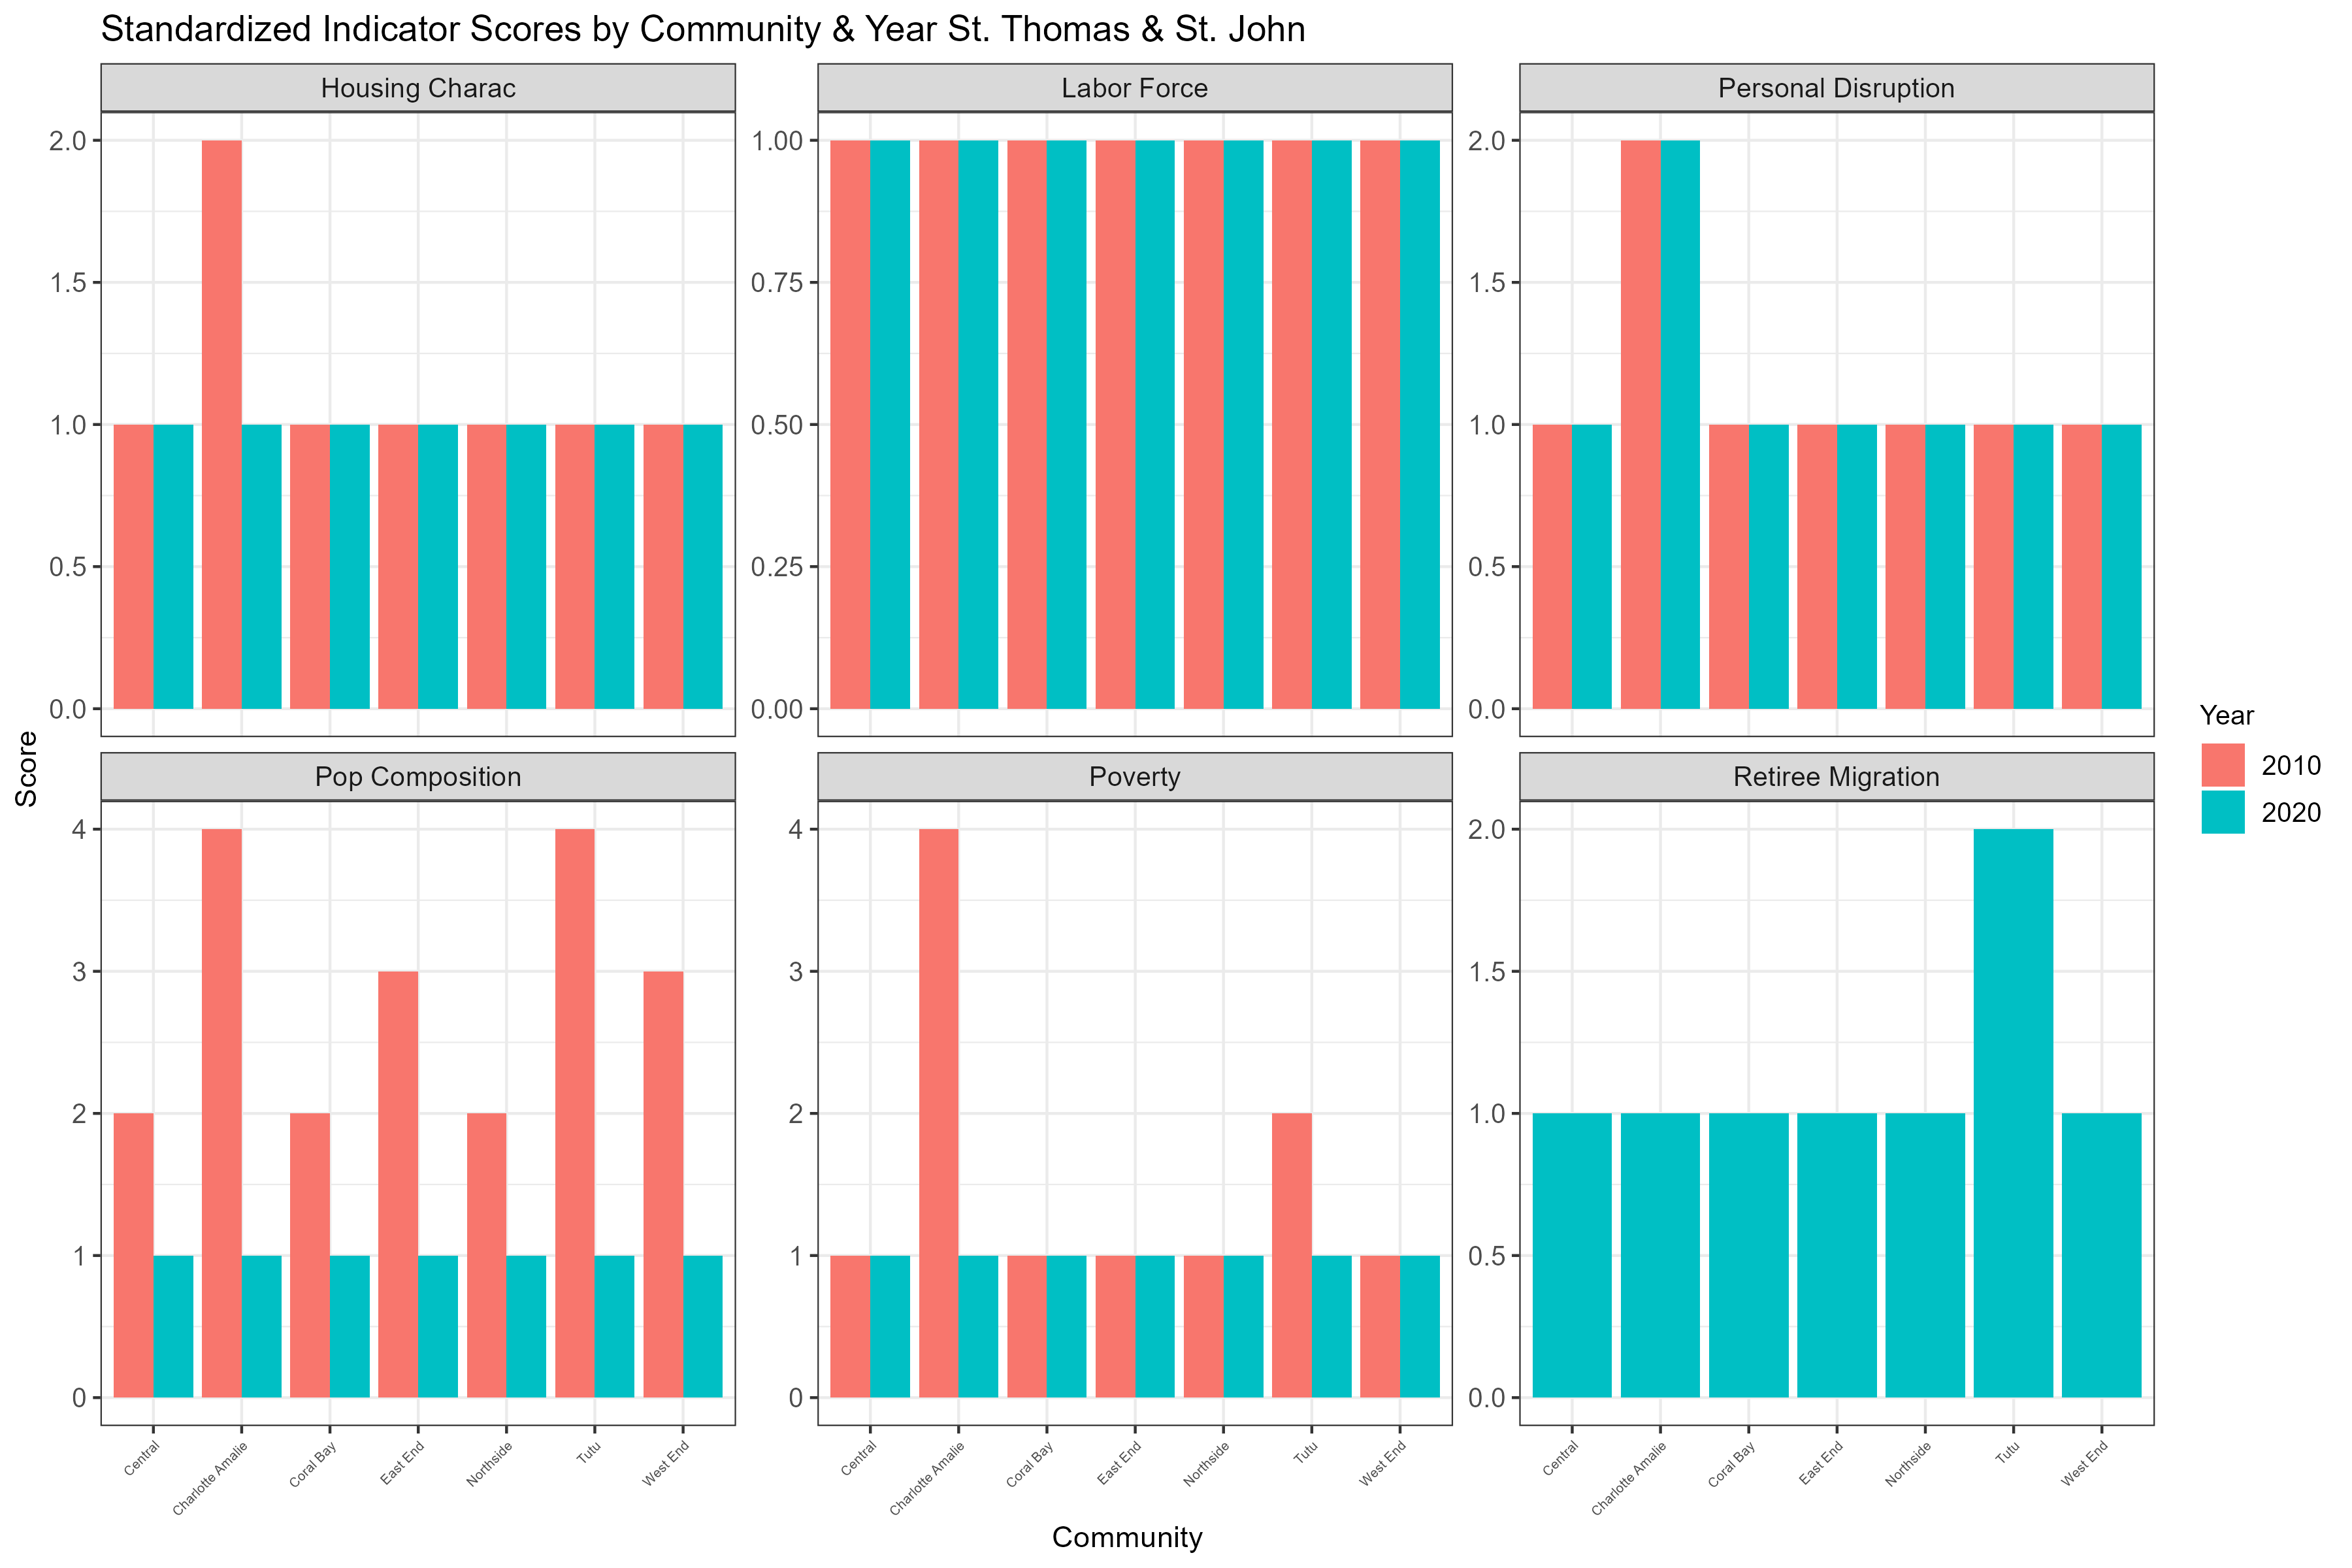
\includegraphics{indicator_plots/CSVI_plots/Faceted_Bar_Plot_St. Thomas & St. John.png}

}

\caption{\label{fig-CSVISTT}}

\end{figure}%

\begin{figure}

\centering{

\captionsetup{labelsep=none}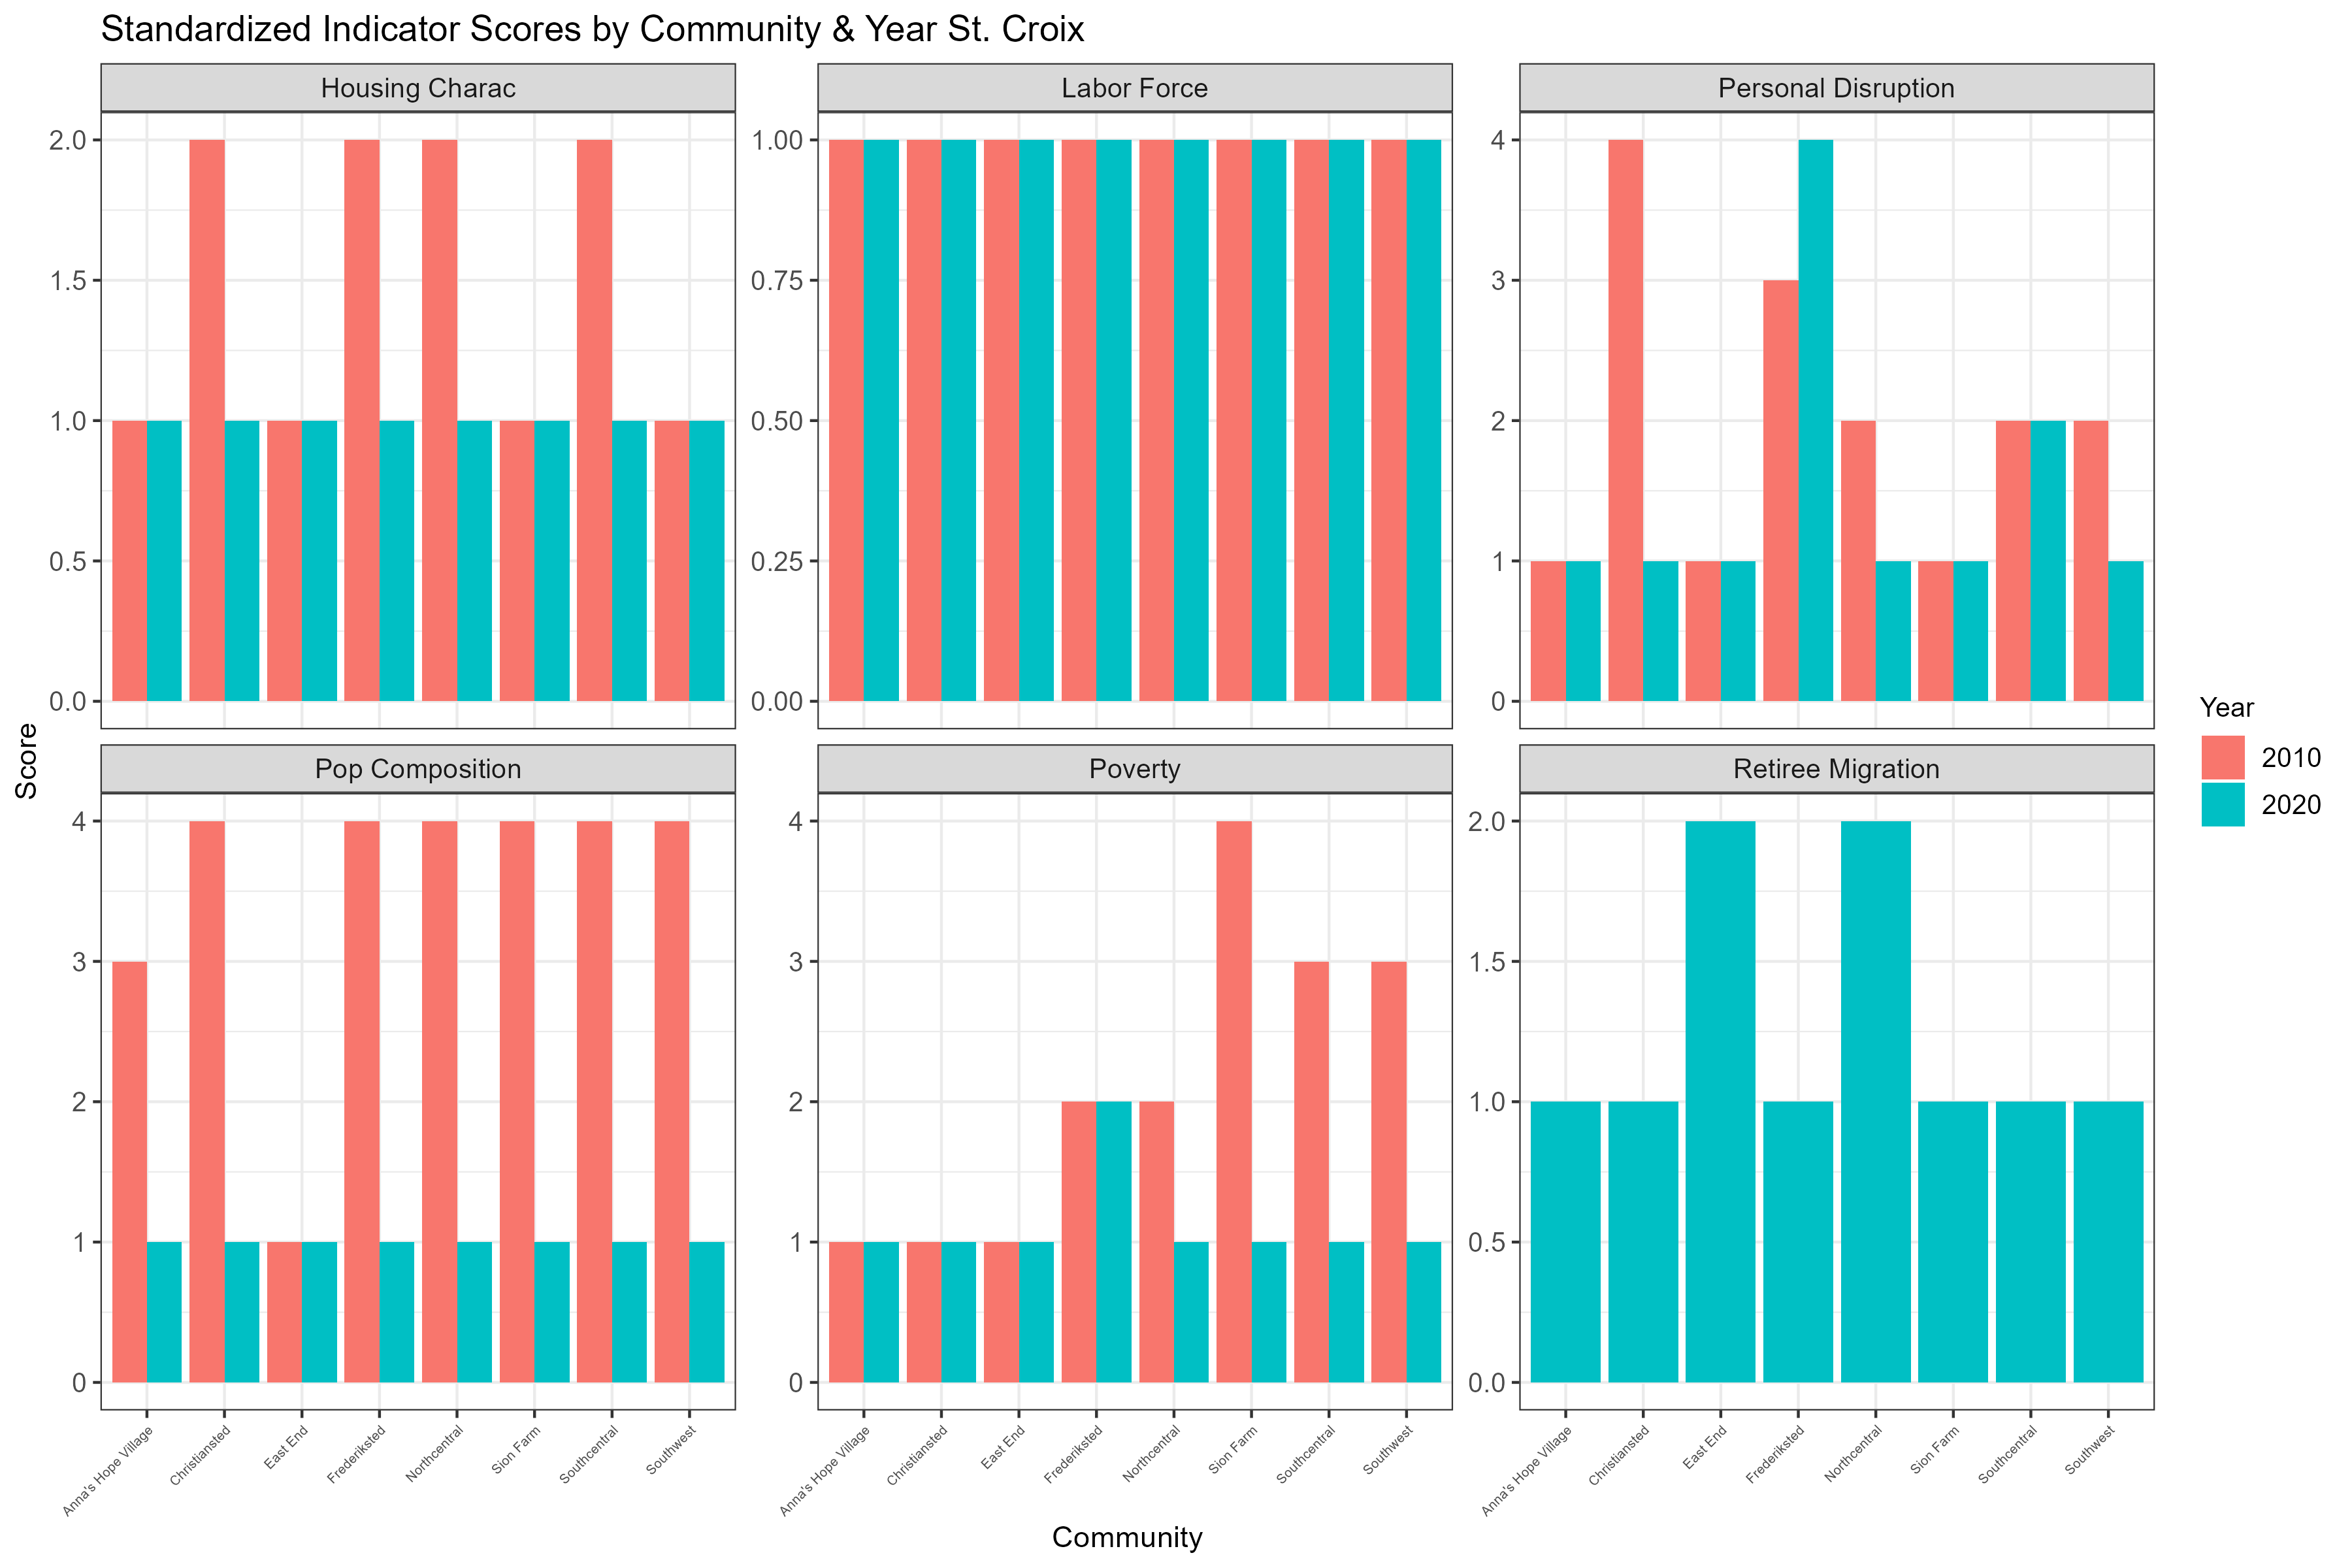
\includegraphics{indicator_plots/CSVI_plots/Faceted_Bar_Plot_St. Croix.png}

}

\caption{\label{fig-CSVISTX}}

\end{figure}%

\section{Engagement and
participation}\label{engagement-and-participation}

\subsection{Recreational landings}\label{recreational-landings}

Recreational catch and effort is a major data gap in the U.S. Caribbean.
The Marine Recreational Intercept Program collected data in Puerto Rico
up until 2016, and in the USVI there are no regular monitoring programs.
The Sea Around Us database esimtates reported catches based on
imputations and assumptions (Pauly and Zeller 2015). In Puerto Rico and
USVI, landings were reconstructed by\ldots(need to fill in). Estimates
suggest that recreational catch has been declining over the last several
decades in Puerto Rico whereas catch has increased over the same period
in the USVI (Figure~\ref{fig-reccatch}).

\begin{figure}

\centering{

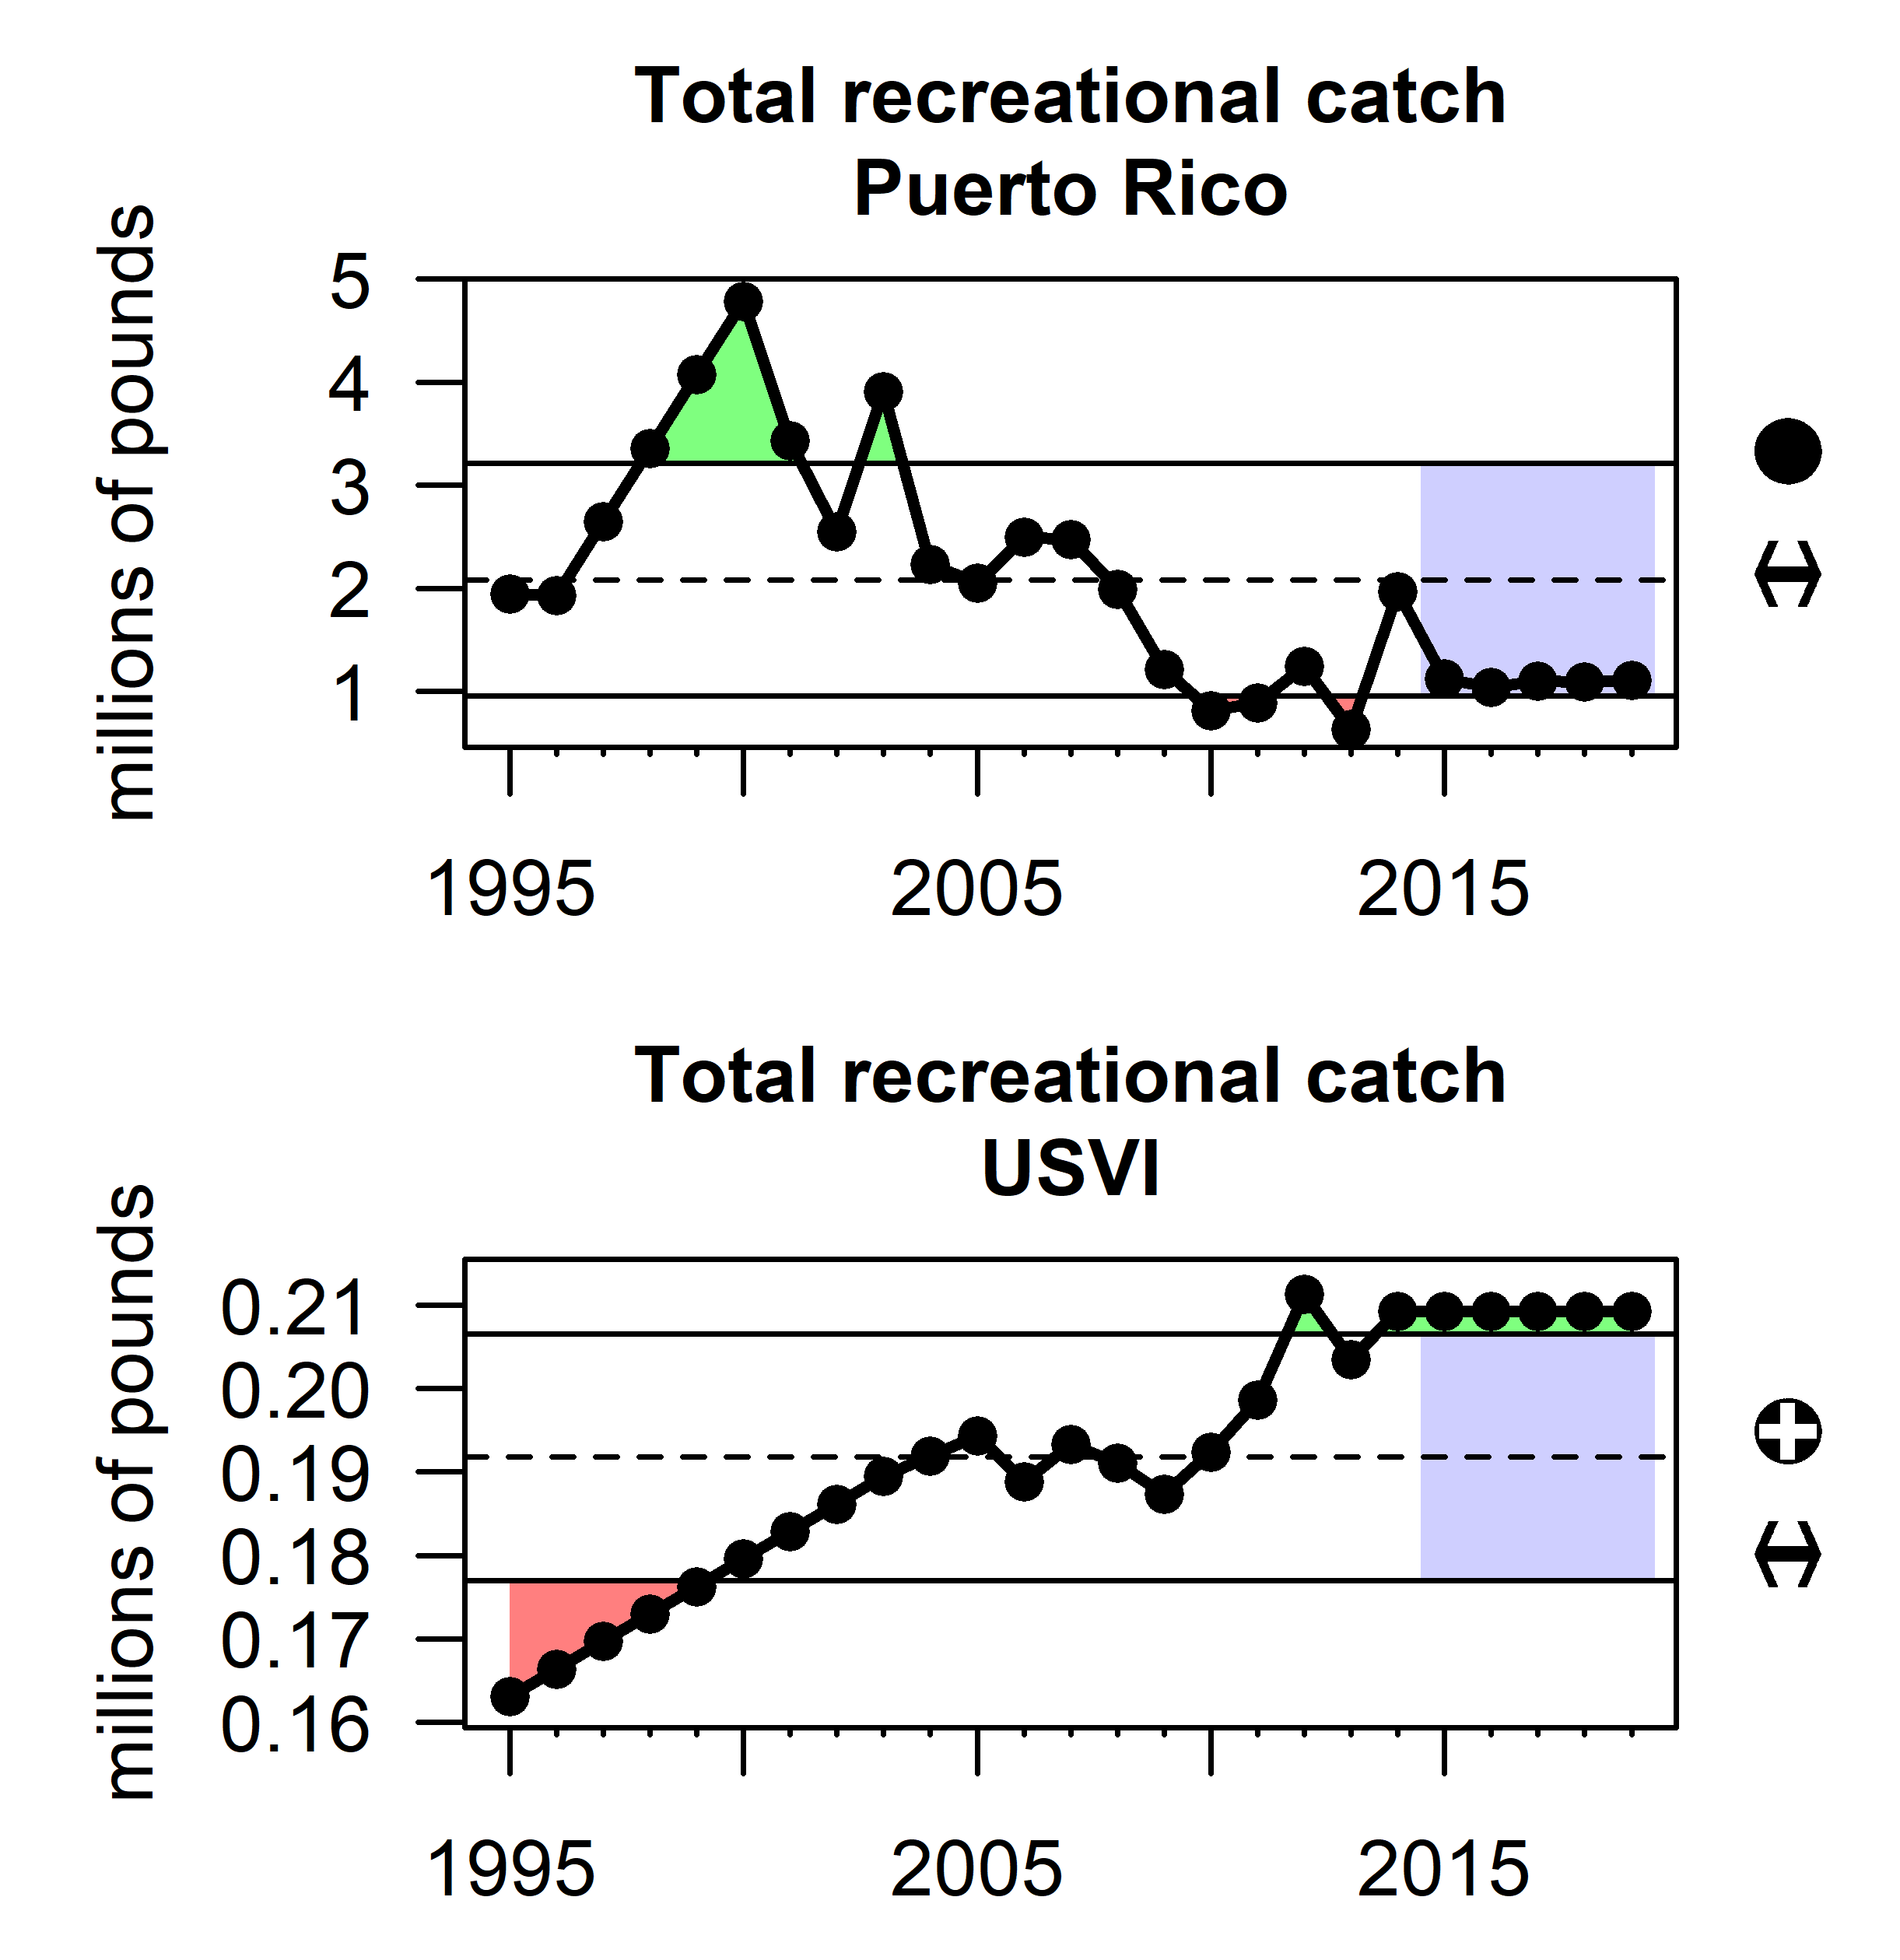
\includegraphics{indicator_plots/total_rec_catch_plot_final.png}

}

\caption{\label{fig-reccatch}Rec catch}

\end{figure}%

\subsection{Commercial fishing engagement and
reliance}\label{commercial-fishing-engagement-and-reliance}

Indicator 28

\begin{figure}

\centering{

\captionsetup{labelsep=none}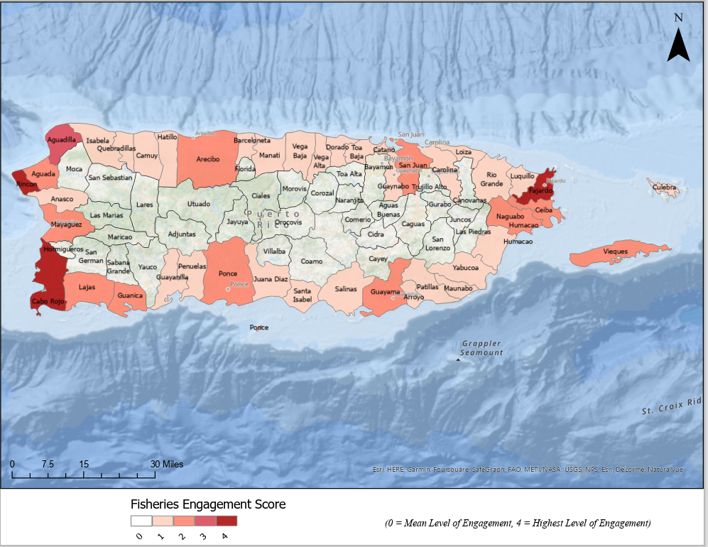
\includegraphics{indicator_plots/PR_comm_fishing_engagement.png}

}

\caption{\label{fig-PRengage}}

\end{figure}%

\begin{figure}

\centering{

\captionsetup{labelsep=none}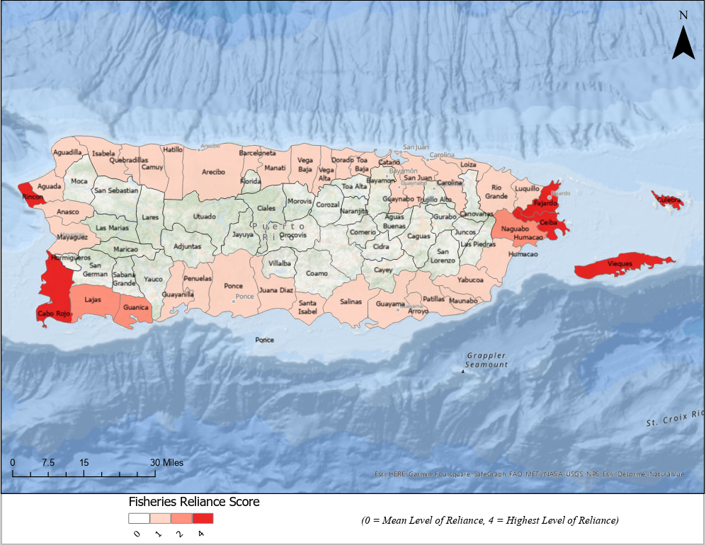
\includegraphics{indicator_plots/PR_comm_fishing_reliance.png}

}

\caption{\label{fig-PRreliance}}

\end{figure}%

\begin{figure}

\centering{

\captionsetup{labelsep=none}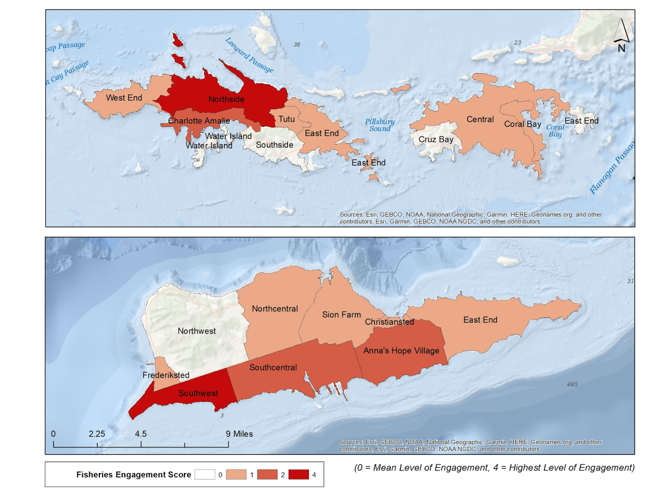
\includegraphics{indicator_plots/USVI_comm_fishing_engagement.png}

}

\caption{\label{fig-USVIengage}}

\end{figure}%

\begin{figure}

\centering{

\captionsetup{labelsep=none}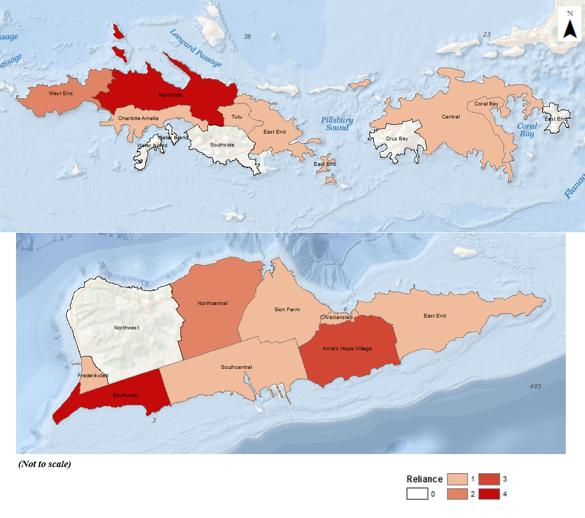
\includegraphics{indicator_plots/USVI_comm_fishing_reliance.png}

}

\caption{\label{fig-USVIreliance}}

\end{figure}%

\section{Bycatch reduction}\label{bycatch-reduction}

\subsection{Changes in gear type}\label{changes-in-gear-type}

Data on bycatch in the U.S. Caribbean are lacking; there are no bycatch
reporting requirements in the logbook and the region has no observer
programs. The selectivity of gears can be considered as some gear types
are highly selective (e.g.~spearfishing and diving) while other gears
capture a wide range of target and non-target species (cite?). We
calculated the proportion of non-selective gears (traps and nets) from
the Caribbean Commercial Landings database as a proxy for bycatch in the
fisheries. Overall the use of these gear types is decreasing in Puerto
Rico and St.~Croix while it is increasing in St.~Thomas and St.~John
(Figure~\ref{fig-bycatch}).

\begin{figure}

\centering{

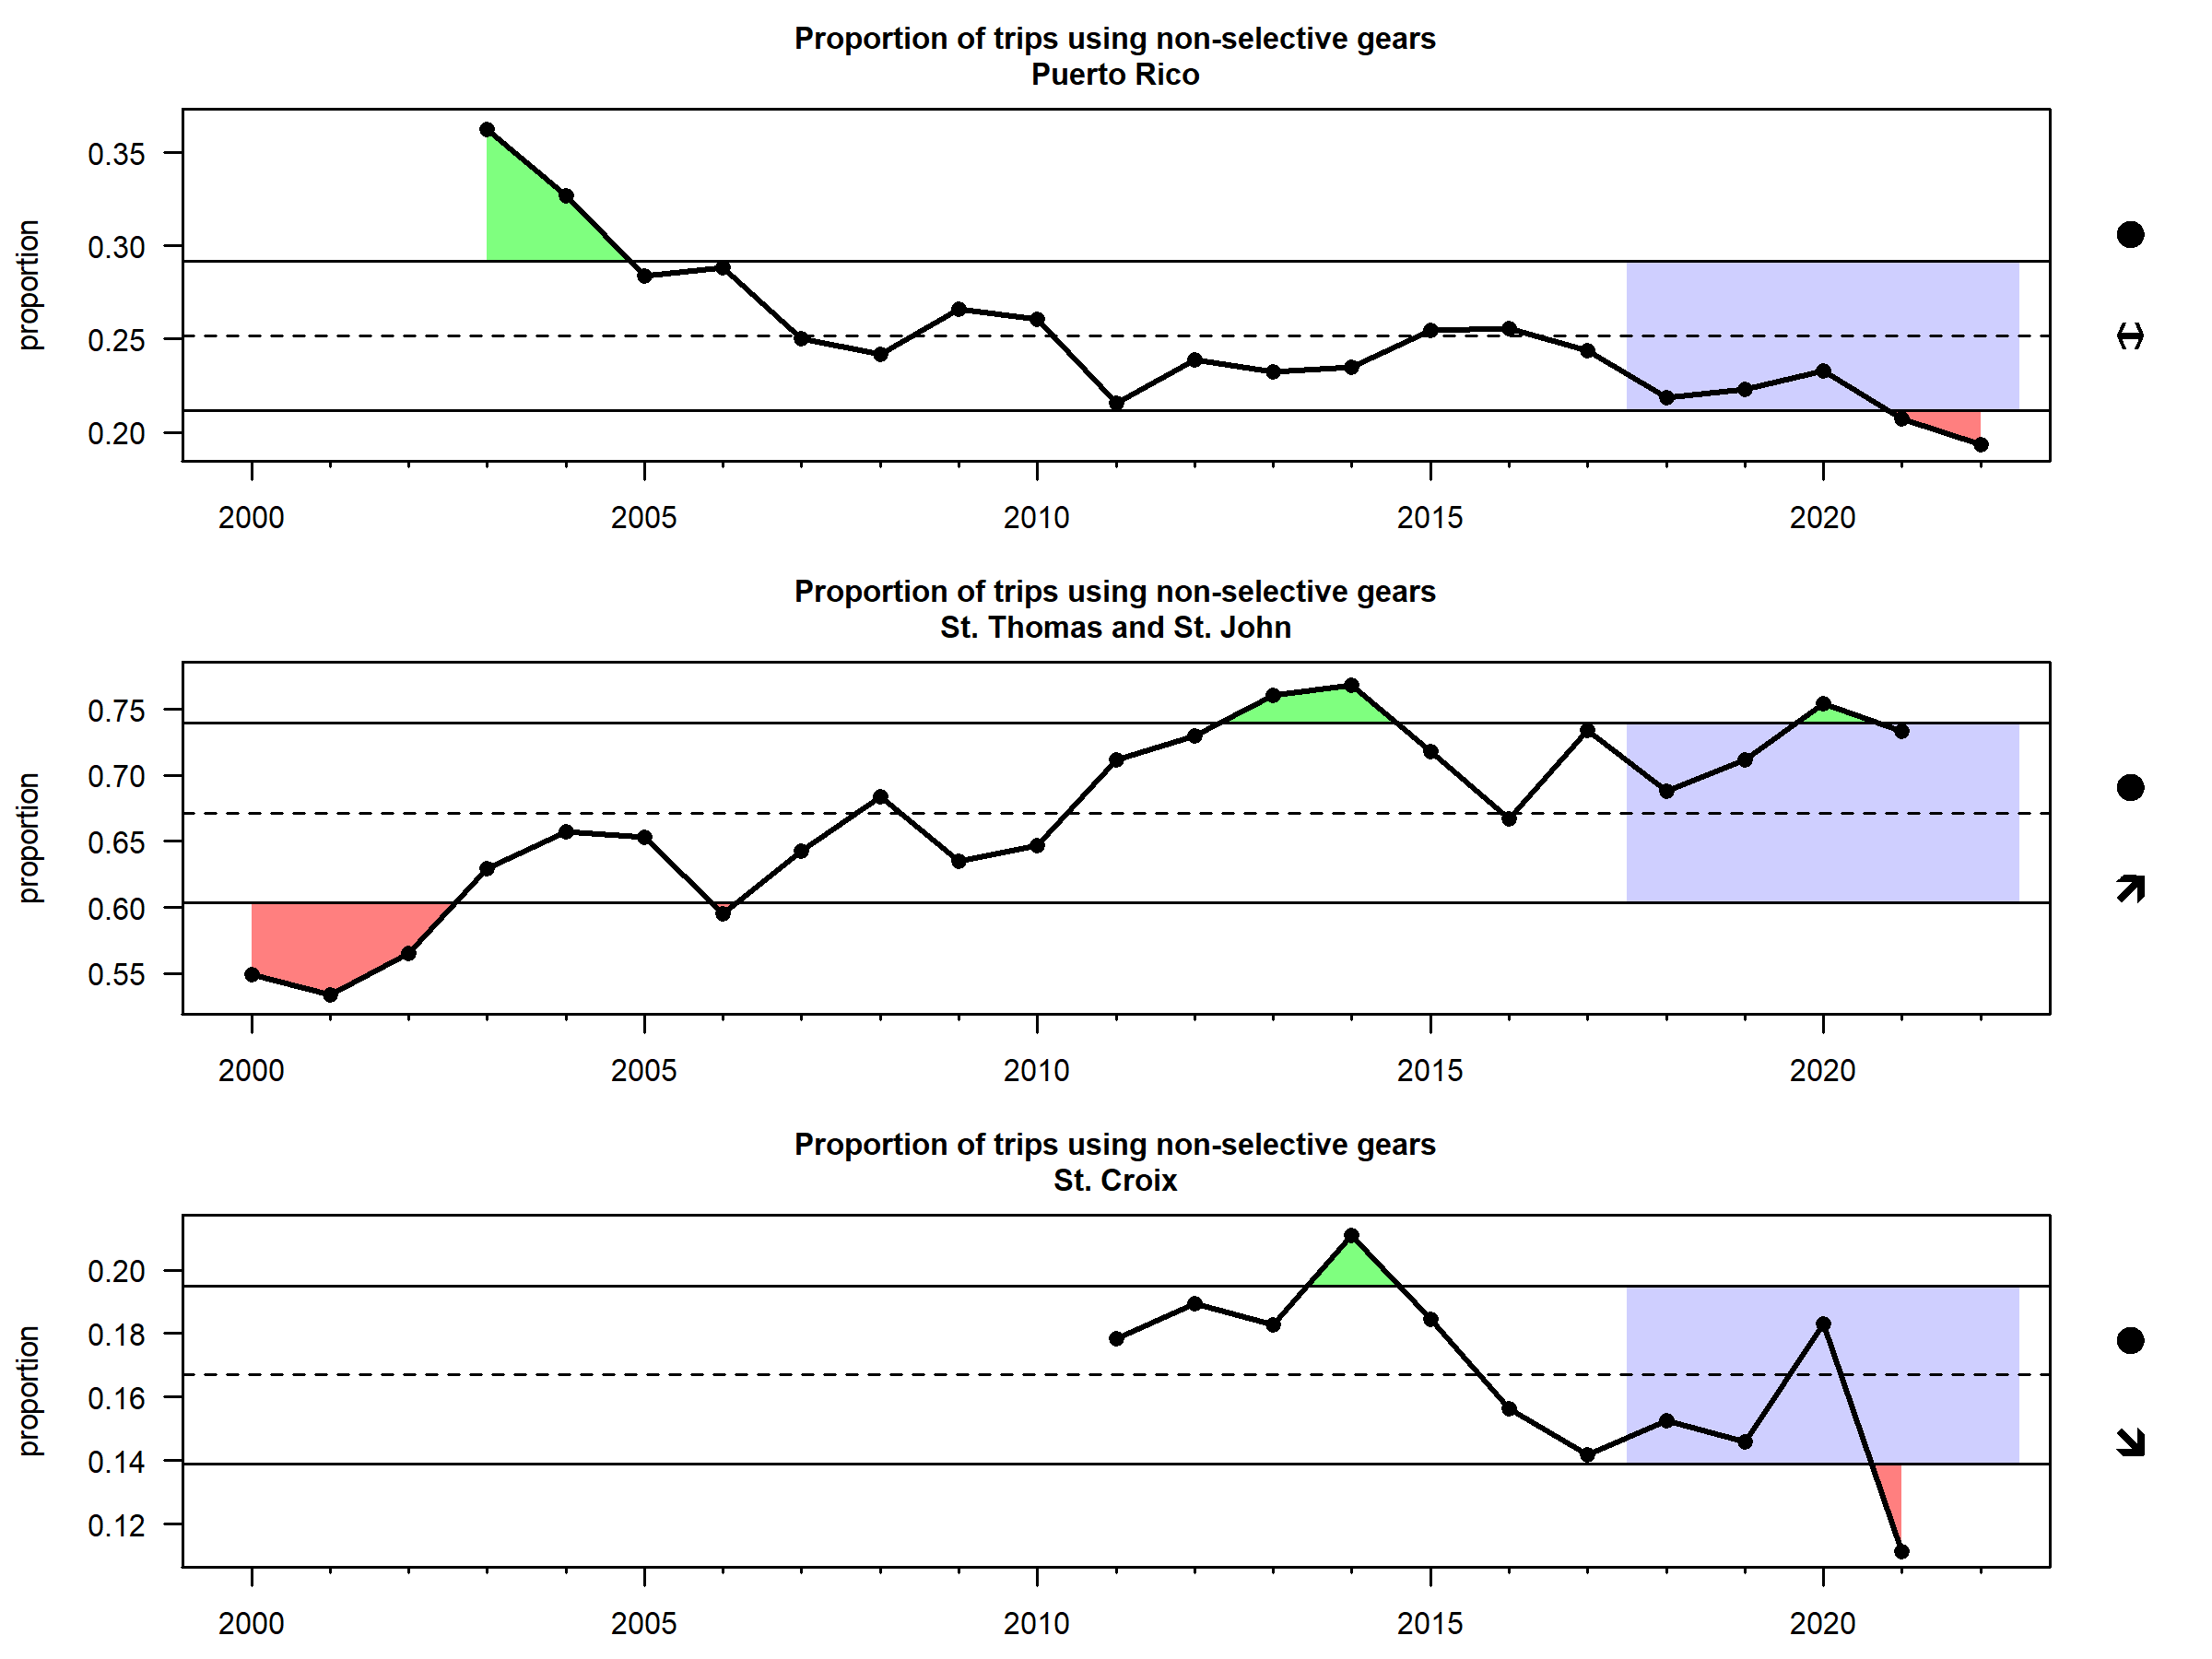
\includegraphics{indicator_plots/prop_trips_bycatch_plot_final.png}

}

\caption{\label{fig-bycatch}Bycatch}

\end{figure}%

\section{Governance}\label{governance}

\subsection{Number of new regulations}\label{number-of-new-regulations}

Indicator 30

\begin{figure}

\centering{

\includegraphics{indicator_plots/FRsection_plot_final.png}

}

\caption{\label{fig-FR}Regulations}

\end{figure}%

\subsection{Percent of species with informative catch
limits}\label{percent-of-species-with-informative-catch-limits}

U.S. Caribbean fisheries are highly diverse; over 300 individual species
have been recorded in the landings database and there are 54 stocks or
complexes within the three Island-based Fishery Management Plans. At the
same time, the region is extremely data-limited, with high uncertainty
in landings data and lacking reliable indices of abundance, and most
annual catch limits are derived using Tier 3 control rules (based on
average landings). The percentage of stocks or complexes with annual
catch limits informed by stock assessments is a useful indicator for
tracking progress toward more robust management advice in the region. In
recent years, progress has been made and several stock assessments have
been accepted for management advice (Figure~\ref{fig-tier3}).

\begin{figure}

\centering{

\includegraphics{indicator_plots/tier3_plot_final.png}

}

\caption{\label{fig-tier3}Tier 3 plot}

\end{figure}%

\subsection{Number of education and outreach
events}\label{number-of-education-and-outreach-events}

Programs such as MREP (Marine Resource Education Program) and NOAA
SeaGrant have made substantial gains in outreach and education in the
U.S. Caribbean region. MREP is a program developed for fishermen, by
fishermen, and is widely recognized as a key venue for engaging industry
members and building trust. Sea Grant is a federal-academic
collaboration that supports research, education and extension to support
coastal resource conservation, conducting outreach in the form of
workshops and meetings. The number of participants benefitting from MREP
and SeaGrant programs has increased rapidly in recent year. Cumulative
numbers of graduates and attendees are reported because once knowledge
is gained it remains in the fishing community and is also spread by
word-of-mouth (Figure~\ref{fig-outreach}).

\begin{figure}

\centering{

\includegraphics{indicator_plots/outreach_plot_final.png}

}

\caption{\label{fig-outreach}Outreach}

\end{figure}%

\subsection{Number of enforcement
actions}\label{number-of-enforcement-actions}

Indicator 33

\begin{figure}[H]

{\centering \includegraphics{indicator_plots/enforcement_plot_final.png}

}

\caption{Enforcement}

\end{figure}%

\section{Protection of ecosystems}\label{protection-of-ecosystems}

\subsection{Percent coral cover and coral species
diversity}\label{percent-coral-cover-and-coral-species-diversity}

Coral reef ecosystem integrity is a major concern for stakeholders in
the U.S. Caribbean region (Seara et al.~2024). The PRCRMP and TRCMP have
measured benthic cover at fixed transects for over two decades, allowing
for a comparison over time. Coral species richness was calculated based
on the average number of hard coral species per transect, and percent
coral cover is reported by\ldots.(need to fill in). Trends in species
richness for both Puerto Rico and the USVI fluctuate over time with no
clear trend, although there has been a sudden decline in recent years.
Percent coral cover has dropped significantly throughout the 25-year
time period with large declines occurring in 2005 and 2019, coinciding
with major bleaching events (Figure~\ref{fig-coral}).

\begin{figure}

\centering{

\includegraphics{indicator_plots/coral_spprichness_cover_plot_final.png}

}

\caption{\label{fig-coral}Coral}

\end{figure}%

\bookmarksetup{startatroot}

\chapter{Integrated ecosystem
perspectives}\label{integrated-ecosystem-perspectives}

\section{Stoplight plot and other synthesis
stuff}\label{stoplight-plot-and-other-synthesis-stuff}

\bookmarksetup{startatroot}

\chapter{Research recommendations}\label{research-recommendations}

\section{Include data gaps, other discussion
material}\label{include-data-gaps-other-discussion-material}

\bookmarksetup{startatroot}

\chapter{Acknowledgments}\label{acknowledgments}

\section{\texorpdfstring{This repo and GitHub Action was based on the
tutorial by Openscapes
\href{https://github.com/Openscapes/quarto-website-tutorial}{quarto-website-tutorial}
by Julia Lowndes and Stefanie
Butland.}{This repo and GitHub Action was based on the tutorial by Openscapes quarto-website-tutorial by Julia Lowndes and Stefanie Butland.}}\label{this-repo-and-github-action-was-based-on-the-tutorial-by-openscapes-quarto-website-tutorial-by-julia-lowndes-and-stefanie-butland.}

\bookmarksetup{startatroot}

\chapter{Contributors}\label{contributors}

\section{\texorpdfstring{\textbf{Editors}}{Editors}}\label{editors}

Mandy Karnauskas, Carissa Gervasi

\section{\texorpdfstring{\textbf{Contributors}}{Contributors}}\label{contributors-1}

Kelly Montenero, Seann Regan, Amy Freitag, Andrea Chan, Chuanmin Hu,
Erica K. Towle, Laura Jay Grove, Jeremiah Blondeau, Sarah Groves, Shay
Viehman, Nicole Besemer, Juan Agar, Kevin McCarthy, Manoj Shivlani, Mike
Jepson, Adyan Rios, Matt McPherson, Miguel Figuerola, Nicole Angeli,
Sennai Habtes, Dione Swanson, Liajay Rivera

\bookmarksetup{startatroot}

\chapter*{References}\label{references}
\addcontentsline{toc}{chapter}{References}

\markboth{References}{References}

\phantomsection\label{refs}
\begin{CSLReferences}{1}{0}
\bibitem[\citeproctext]{ref-agar2022}
Agar, J., B. Stoffle, M. Shivlani, D. Matos-Caraballo, A. Mastitski, and
F. Martin. 2022. {``One-Year COVID-19 Pandemic Impacts on U.S. Caribbean
Small-Scale Fisheries with a Note on the Puerto Rican Earthquake Swarm
of 2020 and 2021. NOAA Technical Memorandum NMFS-SEFSC-759.''}
\url{https://repository.library.noaa.gov/view/noaa/47711}.

\bibitem[\citeproctext]{ref-froese2024}
Froese, R, and D Pauly. 2024. {``FishBase.''}
\href{https://www.fishbase.org}{www.fishbase.org}.

\bibitem[\citeproctext]{ref-hu2012}
Hu, Chuanmin, Zhongping Lee, and Bryan Franz. 2012. {``Chlorophyll
Aalgorithms for Oligotrophic Oceans: A Novel Approach Based on
Three-Band Reflectance Difference.''} \emph{Journal of Geophysical
Research: Oceans} 117 (C1). \url{https://doi.org/10.1029/2011JC007395}.

\bibitem[\citeproctext]{ref-knapp2010}
Knapp, Kenneth R., Michael C. Kruk, David H. Levinson, Howard J.
Diamond, and Charles J. Neumann. 2010. {``The International Best Track
Archive for Climate Stewardship (IBTrACS),''} March.
\url{https://doi.org/10.1175/2009BAMS2755.1}.

\bibitem[\citeproctext]{ref-deleivamoreno2000}
Leiva Moreno, J. I. de, V. N. Agostini, J. F. Caddy, and F. Carocci.
2000. {``Is the Pelagic-Demersal Ratio from Fishery Landings a Useful
Proxy for Nutrient Availability? A Preliminary Data Exploration for the
Semi-Enclosed Seas Around Europe.''} \emph{ICES Journal of Marine
Science} 57 (4): 1091--1102.
\url{https://doi.org/10.1006/jmsc.2000.0705}.

\bibitem[\citeproctext]{ref-puertoricodepartmentofnaturalandenvironmentalresources2019}
Natural, Puerto Rico Department of, and Environmental Resources. 2019.
{``Puerto Rico Long-Term Coral Reef Monitoring Program Database
Compilation: Substrate Cover Percent, Octocoral Colony Counts, Macro
Invertebrate Densities, Fish Densities, and Fish Biomass from 1999 to
2023 (NCEI Accession 0204647). NOAA National Centers for Environmental
Information. Dataset.
Https://Www.ncei.noaa.gov/Archive/Accession/0204647. Accessed
2/6/2024.''}

\bibitem[\citeproctext]{ref-noaacoralreefwatch2019}
NOAA Coral Reef Watch. 2019. \emph{NOAA Coral Reef Watch 5km Regional
Virtual Stations Degree Heating Weeks V3.1 Jan 1, 1985 - Dec 31, 2023.
Silver Spring, MD. USA: NOAA Coral Reef Watch. Data Set Accessed
2024-10-31 at Https://Coralreefwatch.noaa.gov/Product/Vs/Data.php}.

\bibitem[\citeproctext]{ref-pauly2015}
Pauly, D, and D Zeller. 2015. \emph{Sea Around Us Concepts, Design and
Data}. Sea Around Us, Institute for the Oceans; Fisheries, University of
British Columbia, Vancouver, Canada.
\href{https://www.seaaroundus.org}{www.seaaroundus.org}.

\bibitem[\citeproctext]{ref-reynolds2007}
Reynolds, Richard W., Thomas M. Smith, Chunying Liu, Dudley B. Chelton,
Kenneth S. Casey, and Michael G. Schlax. 2007. {``Daily
High-Resolution-Blended Analyses for Sea Surface Temperature,''}
November. \url{https://doi.org/10.1175/2007JCLI1824.1}.

\bibitem[\citeproctext]{ref-rochet2003}
Rochet, Marie-Joëlle, and Verena M Trenkel. 2003. {``Which Community
Indicators Can Measure the Impact of Fishing? A Review and Proposals.''}
\emph{Canadian Journal of Fisheries and Aquatic Sciences} 60 (1):
86--99. \url{https://doi.org/10.1139/f02-164}.

\bibitem[\citeproctext]{ref-seara2024}
Seara, Tarsila, Stacey M. Williams, Kiara Acevedo, Graciela
Garcia-Molliner, Orian Tzadik, Michelle Duval, and Juan J. Cruz-Motta.
2024. {``Development and Analyses of Stakeholder Driven Conceptual
Models to Support the Implementation of Ecosystem-Based Fisheries
Management in the U.S. Caribbean.''} \emph{PLOS ONE} 19 (5): e0304101.
\url{https://doi.org/10.1371/journal.pone.0304101}.

\bibitem[\citeproctext]{ref-smith2011}
Smith, Steven G., Jerald S. Ault, James A. Bohnsack, Douglas E. Harper,
Jiangang Luo, and David B. McClellan. 2011. {``Multispecies Survey
Design for Assessing Reef-Fish Stocks, Spatially Explicit Management
Performance, and Ecosystem Condition.''} \emph{Fisheries Research} 109
(1): 25--41. \url{https://doi.org/10.1016/j.fishres.2011.01.012}.

\bibitem[\citeproctext]{ref-sumy2020}
Sumy, Danielle F., Russ Welti, and Michael Hubenthal. 2020.
{``Applications and Evaluation of the IRIS Earthquake Browser: A
Web{-}Based Tool That Enables Multidimensional Earthquake
Visualization.''} \emph{Seismological Research Letters} 91 (5):
2922--35. \url{https://doi.org/10.1785/0220190386}.

\bibitem[\citeproctext]{ref-wang2019}
Wang, Menghua, Chuanmin Hu, Brian B. Barnes, Gary Mitchum, Brian
Lapointe, and Joseph P. Montoya. 2019. {``The Great Atlantic
{\emph{Sargassum}} Belt.''} \emph{Science} 365: 83--87.
\url{https://www.science.org/doi/10.1126/science.aaw7912}.

\bibitem[\citeproctext]{ref-wang2009}
Wang, Menghua, SeungHyun Son, and Lawrence W. Harding Jr. 2009.
{``Retrieval of Diffuse Attenuation Coefficient in the Chesapeake Bay
and Turbid Ocean Regions for Satellite Ocean Color Applications.''}
\emph{Journal of Geophysical Research: Oceans} 114 (C10).
\url{https://doi.org/10.1029/2009JC005286}.

\end{CSLReferences}


\backmatter

\end{document}
